% An explicit nonlocal game of quantum value one that needs exponential entanglement
% Build: pdflatex main && bibtex main && pdflatex main && pdflatex main
\documentclass[11pt,a4paper]{article}

\usepackage[utf8]{inputenc}
\usepackage{amsmath,amssymb,amsthm,mathtools}
\usepackage[margin=1.05in]{geometry}
\usepackage{booktabs}
\usepackage{longtable}
\usepackage{enumitem}
\usepackage[expansion=false]{microtype}
\setlength{\emergencystretch}{2em}
\usepackage{xcolor}
\usepackage{tikz}
\usetikzlibrary{arrows.meta,calc,positioning,fit,backgrounds}
\usepackage{caption}
\captionsetup{font=small,labelfont=bf}
\usepackage{aliascnt}
\usepackage[colorlinks=true,linkcolor=blue!50!black,citecolor=blue!50!black,urlcolor=blue!50!black]{hyperref}
\usepackage[capitalise,nameinlink]{cleveref}

% ---------- theorem environments (one shared counter, numbered within sections) ----------
\newcommand{\sharedtheorem}[2]{\newaliascnt{#1}{theorem}\newtheorem{#1}[#1]{#2}\aliascntresetthe{#1}}
\theoremstyle{plain}
\newtheorem{theorem}{Theorem}[section]
\sharedtheorem{proposition}{Proposition}
\sharedtheorem{corollary}{Corollary}
\sharedtheorem{lemma}{Lemma}
\sharedtheorem{question}{Question}
\theoremstyle{definition}
\sharedtheorem{definition}{Definition}
\sharedtheorem{example}{Example}
\theoremstyle{remark}
\sharedtheorem{remark}{Remark}
\crefname{question}{Question}{Questions}
\crefname{example}{Example}{Examples}
% lettered theorems of the introduction
\theoremstyle{plain}
\newtheorem*{theoremA}{Theorem A}
\newtheorem*{theoremB}{Theorem B}
\newtheorem*{theoremC}{Theorem C}
\newtheorem*{theoremD}{Theorem D}
\newtheorem*{theoremE}{Theorem E}
\newtheorem*{theoremF}{Theorem F}

% ---------- shared macros (use these; do not redefine) ----------
\DeclareMathOperator{\Tr}{Tr}            % unnormalized trace
\DeclareMathOperator{\tr}{tr}            % normalized trace tr = Tr/d
\DeclareMathOperator{\Area}{Area}
\DeclareMathOperator{\Sym}{Sym}
\DeclareMathOperator{\FSym}{FSym}
\DeclareMathOperator{\GL}{GL}
\DeclareMathOperator{\hlp}{hlp}          % hyperlinear profile
\DeclareMathOperator{\rank}{rank}
\DeclareMathOperator{\supp}{supp}
\DeclareMathOperator{\sgn}{sgn}
\newcommand{\GP}{G_{\mathrm P}}          % the Pauli configuration-lamp group
\newcommand{\GPp}{G_{\mathrm P}^{+}}     % G_P extended by the ray swap iota
\newcommand{\EV}{E_V}                    % central product of Pauli lamps
\newcommand{\RP}{R_{\mathrm P}}          % the 27-word certificate
\newcommand{\Pres}{\mathcal P}           % the EGamma_0 presentation
\newcommand{\Ent}{\mathcal E}            % entanglement cost E(G,eps): least local dimension
\newcommand{\Entme}{\mathcal E^{\mathrm{me}}} % ... on a maximally entangled state
\newcommand{\Gsv}{G_{\mathrm{SV}}}       % the Slofstra--Vidick game
\newcommand{\U}{\mathrm U}
\newcommand{\F}{\mathbb F}
\newcommand{\Z}{\mathbb Z}
\newcommand{\N}{\mathbb N}
\newcommand{\C}{\mathbb C}
\newcommand{\R}{\mathbb R}
\newcommand{\T}{\mathbb T}               % the circle R/2piZ
\newcommand{\E}{\mathbb E}               % expectation
\newcommand{\fn}[1]{\lVert #1\rVert_f}   % normalized Hilbert-Schmidt norm (Tr A^*A/d)^{1/2}
\newcommand{\hs}[1]{\lVert #1\rVert_2}   % unnormalized Hilbert-Schmidt norm (Tr A^*A)^{1/2}
\newcommand{\tn}[1]{\lVert #1\rVert_1}   % trace norm
\newcommand{\op}[1]{\lVert #1\rVert_{\mathrm{op}}} % operator norm
\newcommand{\norm}[1]{\lVert #1\rVert}
\newcommand{\abs}[1]{\lvert #1\rvert}
\newcommand{\ip}[2]{\langle #1,#2\rangle}
\newcommand{\eps}{\varepsilon}
\newcommand{\dH}{\delta_{H}}             % Dehn function of Houghton's group H_3
\newcommand{\omq}{\omega_{q}}
\newcommand{\omqa}{\omega_{qa}}
\newcommand{\omqc}{\omega_{qc}}
\newcommand{\hlps}{\hlp^{\rho}}          % state-weighted profile hlp^rho(w;e)
\newcommand{\hS}{h^{S}}                  % entropy profile
\newcommand{\bfun}{\beta}                % the factor beta(eps)=2^{-4(24+loglog(1/eps))^2}

\hypersetup{pdftitle={An explicit nonlocal game of quantum value one that needs exponential entanglement},
  pdfauthor={Nidhal Mghirbi and Seth Douglas}}

\title{An explicit nonlocal game of quantum value one\\ that needs exponential entanglement}
\author{Nidhal Mghirbi \and Seth Douglas}
\date{Version 1.0.0, October 2026}

\begin{document}
\maketitle

\begin{abstract}
How much entanglement does near-optimal play of a two-player nonlocal game require? We give an explicit binary linear system game,
with $1687$ equations in $1993$ variables and at most three variables in each equation, whose quantum value is one, and in which every
strategy that wins with probability $1-\eps$ needs entanglement entropy $\eps^{-1+o(1)}$, hence local dimension $\exp(\eps^{-1+o(1)})$.
The same bound holds for the entanglement of formation of mixed strategies, and a strategy on a maximally entangled state of local
dimension $\exp(C\eps^{-1}\log(1/\eps))$ suffices, so the exponent is sharp. For explicit two-player games of quantum value one, the best
previous lower bound was polynomial in $1/\eps$.

The game comes from a finitely generated, elementary amenable group: a lamplighter whose lamps are Pauli pairs indexed by finite sets
of points on the three rays on which Houghton's group acts. Exponentially many of these pairs share one central involution, yet the
relation that any two of them commute can be derived from a fixed finite set of relations in a number of steps only quasi-polynomial in
the number of points. Two tools may be of independent use. The first counts qubits from approximate
Pauli relations measured in an arbitrary state, with the errors of different pairs adding in squares. The second identifies, in both
directions and at the natural precision $\sqrt\eps$, the near-optimal strategies of a linear system game with approximate representations
of its solution group measured in the players' actual state, so that no power of $\eps$ is lost by passing to a flat state. The same tools
give sharp rates for two earlier examples: the CHSH$(n)$ games need $\Theta(\min(n,1/\eps))$ ebits, and the linear system game of
Slofstra and Vidick needs local dimension $\Theta(\eps^{-1/2})$.
\end{abstract}

\vspace{0.4em}
\noindent{\small The authors developed this work with AI models from more than one developer and take responsibility for every claim. How
the work was done, and what the machine checks cover, is described in the section ``How this work was done'', before the appendices.}


{\small\setcounter{tocdepth}{1}\tableofcontents}

%======================================================================
\section{Introduction}\label{sec:intro}
%======================================================================

In a two-player nonlocal game a referee sends a question to each of two players, who cannot communicate, and they win if their answers
satisfy a fixed predicate. Players who share an entangled state can sometimes win with a probability that no classical strategy reaches,
and for some games the best winning probability, the \emph{quantum value} $\omq(G)$, is approached only by strategies of ever larger
dimension. For such a game the basic quantitative question is how much entanglement near-optimal play needs. Lower bounds on it are
dimension witnesses: from the winning statistics alone, they certify that the players share a large entangled state. Write $\Ent(G,\eps)$
for the least local dimension of a strategy that wins with probability at least $\omq(G)-\eps$. How fast does $\Ent(G,\eps)$ grow as $\eps\to0$?

The question has a short history. For two-player games of quantum value one, the first explicit examples gave polynomial growth.
Slofstra and Vidick built a linear system game with $c\,\eps^{-1/6}\le\Ent(G,\eps)\le C\eps^{-1/2}$ and wrote that they did not expect the
inverse polynomial scaling to be optimal~\cite{SV18}. Slofstra then reached $\exp(\eps^{-c})$ for a game of commuting-operator value
one, and noted that it is not clear whether its quantum value is one, in part because his group is not known to be hyperlinear and in
part because of limitations of the embedding theorem of~\cite{Slo20} that he used~\cite{Slo18}. Games with super-polynomial growth
are known with three players~\cite{JLV20}, and for two players when the value is not one~\cite{Col20}. There is also a uniform obstruction.
Deciding whether $\omq(G)=1$ is $\Pi_2$-complete~\cite[Thm.~1.1]{MNY22}, while for fixed $D$ and $k$ it is decidable, by
Tarski--Seidenberg, whether some strategy of local dimension at most $D$ wins with probability at least $1-1/k$; so no total computable
function of the game and the precision bounds $\Ent(G,\eps)$ for all games of quantum value one. This names no game and gives no rate
for any one game. Dykema, Paulsen and Prakash showed, through correlation functions of graphs, that
the set of quantum correlations is not closed already for five questions and two answers per player~\cite{DPP19}, so that approximating
some limits of finite-dimensional correlations needs unbounded dimension. \Cref{tab:known}
collects the explicit bounds.

\subsection{The result}

We give an explicit two-player game of quantum value one in which every near-optimal strategy needs exponential entanglement, and we
determine the exponent. Throughout, $\bfun(\eps)=2^{-4(24+\log\log(1/\eps))^2}$; this is $\eps^{o(1)}$ as $\eps\to0$. Logarithms are to
base two.

\begin{theoremA}
There is a binary linear system game $G$, with $1687$ equations in $1993$ variables and at most three variables in each equation, such that
$\omq(G)=1$ and no finite-dimensional strategy wins $G$ with certainty, and there are explicit constants $c,C,\eps_0>0$ with the
following properties for $0<\eps\le\eps_0$.
\begin{enumerate}[label=(\roman*),itemsep=1pt]
\item Every strategy that wins $G$ with probability at least $1-\eps$ has entanglement entropy
\[
S(\rho_B)\ \ge\ c\,\eps^{-1}\,\bfun(\eps),
\]
and hence Schmidt rank, and local dimension, at least $2^{c\,\eps^{-1}\bfun(\eps)}$. For $0<\eps\le\eps_0/2$ the same lower bound,
with $c/4$ in place of $c$, holds for the entanglement of formation of every mixed strategy.
\item Some strategy that wins with probability at least $1-\eps$ uses a maximally entangled state of local dimension at most
$\exp\bigl(C\eps^{-1}\log(1/\eps)\bigr)$.
\end{enumerate}
In particular $\log\Ent(G,\eps)=\eps^{-1+o(1)}$, and the same holds for the least entanglement entropy and for strategies on maximally
entangled states.
\end{theoremA}

The precise statement is \cref{thm:main}, with $c=4.9\cdot10^{-34}$, $C=7.4\cdot10^{10}$ and $\eps_0=2^{-5500}$; these values are far
from optimal. \Cref{box:game} describes the game. To our knowledge $G$ is the first explicit two-player game
of quantum value one that needs more than polynomial entanglement, and the first two-player game of value one whose entanglement is pinned
to a scale $\exp(\eps^{-\Theta(1)})$. The lower bound is on the entanglement \emph{entropy}, so it counts ebits and not only dimensions:
near-optimal play of $G$ consumes $\eps^{-1+o(1)}$ ebits, whatever the shape of the shared state.

\begin{table}[t]
\centering
\footnotesize\setlength{\tabcolsep}{3.5pt}%
\begin{tabular}{@{}llllll@{}}
\toprule
 & players & value & needed & sufficient & remark \\
\midrule
\cite{SV18} & 2 & $\omq=1$ & $c\,\eps^{-1/6}$ & $C\eps^{-1/2}$ & linear system game \\
\cite{MV15} & 2 & $1$ & $c\,\eps^{-1/2}$ & $\eps^{-O(1)}$ & answers of unbounded length \\
\cite{Slo18} & 2 & $\omqc=1$ & $\exp(\eps^{-c})$ & & $\omq=1$ not known \\
\cite{Col20} & 2 & below $1$ & $2^{\Omega(\eps^{-1/8})}$ & $2^{O(\eps^{-1})}$ & within $\eps$ of the value \\
\cite{JLV20} & 3 & $1$ & $2^{\Omega(\eps^{-c})}$ & $2^{O(\eps^{-1})}$ & three players \\
\midrule
Theorem~A & 2 & $\omq=1$ & $\exp(\eps^{-1+o(1)})$ & $\exp(C\eps^{-1}\log\frac1\eps)$ & linear system game; also in ebits \\
\bottomrule
\end{tabular}
\caption{Local dimension needed, and known to suffice, to win with probability $\omega-\eps$, for games whose value $\omega$ is not attained
by finite-dimensional strategies. For Coladangelo's game the bounds concern coming within $\eps$ of its value.
Gao, Yu and Zhi recently gave an explicit linear system game whose commuting-operator
value is one and whose quantum value is below one~\cite{GYZ26}, a different question.}
\label{tab:known}
\end{table}

\paragraph{The group behind the game.} A linear system game is governed by its solution group $\Gamma$, which contains a central involution
$J$: a near-optimal strategy is, up to small errors, a representation of $\Gamma$ in which $J$ acts as $-I$, and the entanglement of the
game is the price of keeping $J$ away from the identity in approximate representations~\cite{SV18}. So we need a group in which $J$ survives
in approximate representations, which gives value one, but only in very large dimension.

Our group $\GP$ is a lamplighter whose lamps sit on configurations rather than on points (\cref{sec:group}, \cref{fig:lamps}). The points
are those of the three rays of Houghton's group $H_3$; a configuration is a finite set of points, written as a binary vector; and the
lighter is a group of affine maps of configurations that permute points, toggle a point, or add one point to another. Each lamp is a Pauli
pair $x_v,z_v$, a copy of the dihedral group of order eight, and the centres $(x_vz_v)^2$ of all lamps are one central involution $J$. On
$N$ points there are $2^N$ configurations, hence $2^N$ Pauli pairs. Yet the generators of the lighter either move points along the rays,
as Houghton's group does, or involve at most two points of a configuration, so any two lamps can be brought together cheaply: their
commutator has area $2^{O(\log^2N)}$ (\cref{thm:pair-area}),
priced by a quasi-polynomial Dehn bound for $H_3$ that we prove in \cref{app:dehn}. The group is elementary amenable, hence hyperlinear,
which removes the first of Slofstra's obstacles. For the second we give explicitly a presentation of the type that the Slofstra--Vidick
reduction needs, with one non-involutive generator, whose $29$ derivations are checked by machine (\cref{sec:game}).

% Figure 1: the three rays, a configuration, and a transporter (introduction).
\begin{figure}[t]
\centering
\begin{tikzpicture}[x=1cm,y=1cm,font=\small,>=Stealth,baseline=(current bounding box.center),
  pt/.style={circle,draw,fill=white,inner sep=0pt,minimum size=5pt},
  on/.style={pt,fill=black},
  lbl/.style={font=\footnotesize,inner sep=1pt}]
\def\u{0.7}
\foreach \i/\ang in {1/0,2/120,3/240}{
  \draw[black!50] (0,0) -- (\ang:4.4*\u);
  \node at (\ang:4.85*\u) {$\cdots$};
  \foreach \j in {1,...,4}{\node[pt] (p\i\j) at (\ang:\j*\u) {};}
}
\node[lbl,anchor=west] at ($(120:4.8*\u)+(0.3,0)$) {ray $2$};
\node[lbl,anchor=west] at ($(240:4.8*\u)+(0.3,0)$) {ray $3$};
\node[lbl,anchor=north] at ($(0:4.8*\u)+(0.1,-0.2)$) {ray $1$};
\foreach \j in {1,...,4}{\node[lbl,anchor=north] at ($(p1\j)+(0,-0.16)$) {$\j$};}
\node[on] at (p11) {};
\node[on] at (p13) {};
\node[lbl,anchor=south] at ($(p12)+(0,0.3)$) {$u=e_1+e_3$};
\end{tikzpicture}%
\hspace{1.2cm}%
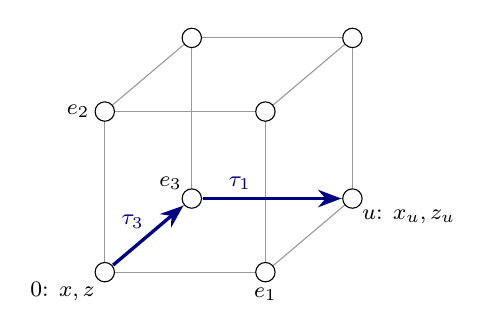
\begin{tikzpicture}[x=0.85cm,y=0.85cm,font=\small,>=Stealth,baseline=(current bounding box.center),
  lamp/.style={circle,draw,fill=white,inner sep=0pt,minimum size=7pt},
  mv/.style={blue!50!black,very thick,->,shorten >=4pt,shorten <=4pt},
  lbl/.style={font=\footnotesize,inner sep=1pt}]
\coordinate (v0) at (0,0);
\coordinate (v1) at (2.4,0);
\coordinate (v2) at (0,2.4);
\coordinate (v12) at (2.4,2.4);
\coordinate (v3) at (1.3,1.1);
\coordinate (v13) at (3.7,1.1);
\coordinate (v23) at (1.3,3.5);
\coordinate (v123) at (3.7,3.5);
\draw[black!40] (v0) -- (v1) -- (v12) -- (v2) -- cycle;
\draw[black!40] (v3) -- (v13) -- (v123) -- (v23) -- cycle;
\draw[black!40] (v0) -- (v3) (v1) -- (v13) (v2) -- (v23) (v12) -- (v123);
\draw[mv] (v0) -- (v3);
\draw[mv] (v3) -- (v13);
\node[lbl,blue!50!black,anchor=south east] at ($(v0)!0.5!(v3)+(-0.02,0.06)$) {$\tau_3$};
\node[lbl,blue!50!black,anchor=south] at ($(v3)!0.3!(v13)+(0,0.08)$) {$\tau_1$};
\foreach \v in {v0,v1,v2,v12,v3,v13,v23,v123}{\node[lamp] at (\v) {};}
\node[lbl,anchor=north east] at ($(v0)+(-0.1,-0.1)$) {$0$: $x,z$};
\node[lbl,anchor=north west] at ($(v13)+(0.1,-0.12)$) {$u$: $x_u,z_u$};
\node[lbl,anchor=north] at ($(v1)+(0,-0.18)$) {$e_1$};
\node[lbl,anchor=east] at ($(v2)+(-0.18,0)$) {$e_2$};
\node[lbl,anchor=south east] at ($(v3)+(-0.1,0.08)$) {$e_3$};
\end{tikzpicture}
\caption{Left: the points of the three rays of Houghton's group and a configuration $u=e_1+e_3$, a finite set of points (filled). Right: the
$2^3$ configurations supported on the points $1,2,3$ of ray~$1$, each carrying a Pauli pair (a circle), with $(x_vz_v)^2=J$ for all $v$. The
transporter $T_u=\tau_1\tau_3$, a word in the generators, carries the configuration $0$ to $u$ (bold path), and conjugation by it carries the
pair $x,z$ at $0$ to the pair $x_u=T_uxT_u^{-1}$, $z_u=T_uzT_u^{-1}$ at $u$. On $N$ points there are $2^N$ pairs, and on the sector where $J$
acts as $-1$ each acts as a qubit.}
\label{fig:lamps}
\end{figure}


\subsection{Why the state must be kept}

A strategy that wins with probability $1-\eps$ controls the players' operators to precision about $\sqrt\eps$, measured in their shared
state: if $\rho$ is Bob's reduced density matrix and $\xi=\rho^{1/2}$, his observables satisfy the relations of the solution group up to
$\sqrt\eps$ in the norm $\hs{Y\xi}=\Tr(Y^*Y\rho)^{1/2}$, and they nearly commute with $\xi$, again to order $\sqrt\eps$. The usual route to a
lower bound then \emph{flattens} the state: it passes to a spectral projection of $\rho$~\cite{SV18}, to a strategy on a maximally entangled
state~\cite{Pad22}, or to the operator norm. Each of these steps costs a power of $\eps$. For linear system games the precision $\sqrt\eps$
becomes $\eps^{1/4}$~\cite[Cor.~5.2]{SV18}; for our game this would give only $\log\Ent(G,\eps)\ge\eps^{-1/2+o(1)}$, the exponent of
maximally entangled strategies halved.

We avoid the loss by never leaving the state. The counting argument below works with the Hilbert--Schmidt vector $\xi$ itself: it
compares quantities measured in one and the same state, and it pays for every change of state with a \emph{state commutator}
$\hs{[Y,\xi]}$, which near-optimal play supplies at precision $\sqrt\eps$. Two results make this precise, and both may be of independent use.

The first is a robust form of the fact that $M$ pairs of anticommuting involutions need $M$ qubits, valid in an arbitrary state, with the
errors of different pairs adding in squares rather than in norms.

\begin{theoremC}[\cref{thm:count,cor:count}]
Let $X_1,\dots,X_M,Z_1,\dots,Z_M$ be involutions on $\C^d$, $M\ge2$, let $\rho$ be a density matrix and $\xi=\rho^{1/2}$. If for all $i\ne j$
\[
\hs{[Z_i,Z_j]\xi},\ \ \hs{[X_i,Z_j]\xi},\ \ \hs{\{X_i,Z_i\}\xi},\ \ \hs{[X_i,\xi]},\ \ \hs{[Z_i,\xi]}\ \le\ \kappa
\]
and $16M\kappa^2\le\frac1{10}$, then $S(\rho)\ge\frac34M$.
\end{theoremC}

The full statement, \cref{thm:count}, bounds $S(\rho)$ from below by a sum over the pairs in which the errors of each pair enter only through sums of
squares. The state commutators cannot be dropped (\cref{ex:commutators-needed}). Stability theorems of Gowers--Hatami type~\cite{GH17} and the
many-qubit tests of Natarajan and Vidick~\cite{NV17} need control of a whole Pauli group; \cref{thm:count} needs only the pairwise relations,
and the $\ell^2$ tolerance is what produces the exponent $1$ in Theorem~A. Pairwise approximate relations with a fixed error per pair allow many
approximate qubits to overlap in a small space~\cite{CRSV17}; \cref{thm:count} is consistent with this, because it charges the errors of all
pairs together, through a sum of squares.

The second result says that for linear system games nothing is lost in either direction when the state is kept. For a finite presentation
and a word $w$, let $\hlps(w;e)$ be the least dimension of a homomorphism $\phi$ from the free group to $\U(d)$ together with a density
matrix $\rho$ such that every relator is $e$-close to the identity in the norm $\hs{(\cdot)\xi}$, every generator has state commutator at
most $e$, and $\hs{(\phi(w)+I)\xi}\le e$ (\cref{def:state-profile}).

\begin{theoremD}[\cref{thm:transfer,thm:return,cor:two-sided}]
Let $G$ be a binary linear system game of quantum value one with solution group $\Gamma$ and central element $J$. There are constants
$C,C'>0$, depending only on the number of equations, the number of variables per equation and the question distribution, such that for
every $\eps>0$
\[
\hlps_\Gamma\bigl(J;C\sqrt\eps\bigr)\ \le\ \Ent(G,\eps)\ \le\ \hlps_\Gamma\bigl(J;C'\sqrt\eps\bigr).
\]
Both directions keep the state: the lower bound uses Bob's reduced state, and the upper bound is realised on the canonical purification of
the state of the model. The same holds for the least entanglement entropy.
\end{theoremD}

For flat models the right-hand inequality is the classical direction of the correspondence of Slofstra and
Vidick~\cite[Prop.~4.4(a)]{SV18}. The left-hand one is their passage from strategies to approximate representations~\cite[Prop.~5.4]{SV18},
stopped before the state is flattened.

\subsection{The profile of the central involution}

On the side of the group, the lower bound of Theorem~A is a statement about approximate representations of $\GP$ in which $J$ is visible.
Let $\hlp(J;\delta,\eps)$ be the least dimension of an $\eps$-representation $\phi$ with $\fn{\phi(J)-I}\ge\delta$, the \emph{hyperlinear
profile} of $J$~\cite{SV18}, and let $\RP$ be the finite certificate of $27$ relations of $\GP$ of \cref{def:RP}.

\begin{theoremB}[\cref{thm:profile}]
Let $R\supseteq\RP$ be a finite set of words in the generators $p,q,t,d,x,z$ of $\GP$ that represent $1$ in $\GP$, and $J=(xz)^2$. There are
constants $c,C>0$, with $C$ depending on the lengths of the words of $R$, such that for $0<\delta\le2$ and $0<\eps\le2^{-1071}\delta$
\[
c\,\delta^2\eps^{-2}\bfun(\eps)\ \le\ \log\hlp_R(J;\delta,\eps)\ \le\ C\,\delta^2\eps^{-2}\log(1/\eps).
\]
The same two-sided bound $\log\hlps_R(J;e)=e^{-2+o(1)}$ holds for the state-weighted profile.
\end{theoremB}

So $\log\hlp(J;\delta,\eps)=\eps^{-2+o(1)}$. By~\cite[Prop.~7.1]{DM-lamps} the group $\GP$ is finitely presented (nothing here uses
this; see \cref{rem:GP-fp}), so it is, to our knowledge, the first finitely presented amenable group with a central involution of
superpolynomial hyperlinear profile. The upper bound comes from \emph{hash models} (\cref{sec:upper}): we keep only the
lamps that a short word lights, on a register of qubits indexed by a random affine hash of the configurations, and a clock handles the
abelian quotient of the lighter. Slofstra's group in~\cite{Slo18} has $\log\hlp\ge c\,\eps^{-a}$ for every $a<\frac12$, and is not known to be
hyperlinear; the sofic group of Slofstra and Vidick has a central involution of polynomial profile~\cite[Prop.~3.2]{SV18}.

\subsection{Two sharp rates}

The same two tools close the gaps in two classical examples, in which the known lower bounds lost a power of $\eps$ by flattening.

The XOR games CHSH$(n)$ of Slofstra~\cite{Slo11} force $n$ pairwise anticommuting observables. Ostrev showed that every nearly optimal
strategy approximately contains the algebraic structure of the canonical optimal one~\cite{Ost16}; the question here is how much
entanglement that forces as a function of the error. Ostrev and Vidick showed that a strategy within
a factor $1-\eps$ of the optimal bias needs $\Omega(\eps^{-1/5})$ ebits, using $n=\Theta(\eps^{-1/5})$, and that every XOR game has an
$\eps$-optimal strategy with $\lceil1/\eps\rceil$ ebits~\cite{OV18}.

\begin{theoremE}[\cref{thm:chsh,cor:chsh-ebits,cor:chsh-ef}]
For $n\ge3$ and $0<\eps\le1$, the least entanglement entropy of a strategy for CHSH$(n)$ whose bias is at least $1-\eps$ times the optimal
bias lies between $10^{-7}\min(n,1/\eps)/6-\frac12$ and $\min(\lfloor n/2\rfloor,\lceil1/\eps\rceil)$; so it is $\Theta(\min(n,1/\eps))$ as
$\min(n,1/\eps)\to\infty$. The least entanglement of formation of a mixed strategy obeys the same bounds, with $10^{-7}/24$ and $\frac14$
in place of $10^{-7}/6$ and $\frac12$.
\end{theoremE}

This improves the exponent $\frac15$ of~\cite{OV18} to the optimal $1$. Slofstra and Vidick built a linear system game $\Gsv$ from a group $K$
whose central involution $c$ has hyperlinear profile between $\eps^{-2/3}$ and $\eps^{-1}$, and gave the bounds
$c\,\eps^{-1/6}\le\Ent(\Gsv,\eps)\le C\eps^{-1/2}$~\cite{SV18}.

\begin{theoremF}[\cref{cor:K-profile,thm:sv-game}]
The hyperlinear profile of $c$ in $K$ is $\Theta(1/\eps)$, for every fixed $\delta$, and $\Ent(\Gsv,\eps)=\Theta(\eps^{-1/2})$.
\end{theoremF}

Here the relations make the spectral measure of one generator, measured in the state, nearly invariant under doubling and under a half-turn
of the circle; averaging over the two inverse branches of the doubling map contracts the Wasserstein-$1$ distance by a factor two, so the
measure is within $\frac{29\pi}2$ times the precision of Haar measure (\cref{prop:K-W1}), while a measure with $d$ atoms is at distance at
least $\pi/(2d)$.

The upper bound $\Ent(\Gsv,\eps)\le C\eps^{-1/2}$ is that of Slofstra and Vidick~\cite[Thm.~1.1]{SV18}. Its proof, through that
of~\cite[Prop.~6.2]{SV18}, lifts approximate representations of $K$ to the solution group by~\cite[Prop.~4.8]{Slo19}, which removes one
non-involutive generator at a time; $K$ has two, and after both removals the image of $c$ is no longer balanced, so the last step of that
proof does not apply as written (\cref{sec:rates-sv}). Only the upper bound is affected: the value one of the game, the lower bounds and
the nontriviality of $J$ do not use this step, and with at most one non-involutive generator the argument is complete. For the explicit
models of $K$ we give a lift that keeps $c$ balanced (\cref{lem:sv-lift}), so~\cite[Thm.~1.1]{SV18} holds as stated.

\subsection{How the proof of Theorem A works}

We describe the lower bound; the upper bound runs the chain backwards using flat approximate models in which the marked involution is
exactly $-I$. \Cref{game:fig-map} in \cref{sec:game}
shows both chains with their constants.

\emph{From the game to a state-weighted model.} A strategy that wins with probability $1-\eps$ gives, on the support of Bob's reduced state
$\rho$, involutions for the variables of the game that satisfy the relations of the solution group $\Gamma$, and commute with $\xi$, up to
$O(\sqrt\eps)$ in the state (\cref{thm:transfer}). This is bookkeeping, but it is the step at which earlier arguments flattened the state.

\emph{From the game to the group.} The game is built from a presentation $\Pres$ of Slofstra's type $E\Gamma_0$ through Slofstra's
embedding, run so that the distinguished involution goes to $-I$ (\cref{app:gadget}), and the $27$ relations of the certificate $\RP$ are
consequences of $\Pres$ of area at most $60$ (\cref{prop:presentation}). So the model of $\Gamma$ restricts to an assignment of unitaries to
the generators $p,q,t,d,x,z$ of $\GP$ satisfying $\RP$ to $O(\sqrt\eps)$ in the state, in which the image of $J$ stays at distance about one
from the identity.

\emph{Lamps on the sector.} On the sector where (the rounded image of) $J$ acts as $-1$, the transported lamps $x_u,z_u$, $u\subseteq\{1,\dots,N\}$,
are $2^N$ approximate Pauli pairs measured in the state: within a pair they nearly anticommute because $(x_uz_u)^2=J=-1$, and across pairs
they nearly commute at a cost of the pair area $\Lambda_N=2^{O(\log^2N)}$ times the precision (\cref{thm:pair-area}). Charging conjugators
through state commutators squares this cost.

\emph{Counting.} Theorem~C applies with $M=2^N$ and $\kappa\approx\Lambda_N^2\sqrt\eps$, as long as $2^N\Lambda_N^4\eps\lesssim1$. Choosing the
largest such $N$ gives $2^N=\eps^{-1+o(1)}$ qubits of entropy on the sector (\cref{thm:sector}), and the sector carries a constant fraction of
the state (\cref{lem:sector-entropy}). This is where the exponent $1$ comes from: precision $\sqrt\eps$, errors adding in squares.

\emph{The upper bound.} The hash models give $\eps$-representations of $\GPp$ with $J\mapsto-I$ exactly in dimension
$\exp(C\eps^{-2}\log(1/\eps))$; they give approximate representations of $\Pres$ with $w\mapsto-I$ and then of $\Gamma$ with $J\mapsto-I$
(the embedding theorem, \cref{thm:embedding} in \cref{app:gadget}), and the return direction of
Theorem~D turns them into strategies on a maximally entangled state that lose with probability $O(\eps^2)$ (\cref{thm:return}).

\subsection{Related work and what is new}

The architecture of the group follows Slofstra's~\cite{Slo18}: a central involution $J$, a family of involutions whose commutators are
$J$ or $1$, exponentially many of them reached by short words, and a transfer of approximate representations along the group.
In~\cite{Slo18} the involutions generate, with $J$, an infinite Clifford group, any two of them anticommuting up to $J$, and they are
reached through the HNN doubling $tzt^{-1}=z^2$; here they form Pauli pairs and are reached through Houghton's group acting on
configurations, which keeps the group amenable. The passage from groups to games is Slofstra's embedding~\cite{Slo19,Slo20} in the explicit form of Slofstra and
Vidick~\cite{SV18}, and the identification of the entanglement of a linear system game with the hyperlinear profile of $J$ is theirs. The
pair-area argument and the hash models adapt our earlier construction for lamps that are copies of $S_3$, where they bound the sofic profile
of an amenable group~\cite{DM-lamps}; nothing in this paper depends on that preprint.

On the analytic side, the Hilbert--Schmidt picture of a shared state, with the reduced state as a factor $\xi$, is the standard form of the
state. Slofstra and Vidick use it for general strategies~\cite{SV18}, and Marrakchi and de la Salle use it to round near-synchronous
strategies~\cite{MdlS23}. The coupling of two spectral measures in one state is Connes' joint distribution of left and right
multiplication~\cite{Con76}. Robust tests of many qubits in the players' state are due to Natarajan and Vidick~\cite{NV17}, through a test
that samples the whole Pauli group; Pauli stability for synchronous strategies is in~\cite{dlS22}; state-dependent anticommutators appear in
the entropic uncertainty relations of Kaniewski, Tomamichel and Wehner~\cite{KTW14}; and rounding to maximally entangled or tracial strategies
is studied in~\cite{Vid22,Pad22,Lin23,MdlS23}.

What is new is the following.
\begin{enumerate}[label=(\arabic*),itemsep=1pt]
\item An explicit two-player game of quantum value one whose near-optimal strategies need $\eps^{-1+o(1)}$ ebits, with a matching upper
bound (Theorem~A).
\item An elementary amenable group with a central involution whose hyperlinear profile is $\exp(\eps^{-2+o(1)})$, two-sided, for every
finite set of valid relations that contains $\RP$ (Theorem~B), and a self-contained proof, from Johnson's presentation, of a
quasi-polynomial Dehn bound for Houghton's group $H_3$ (\cref{app:dehn}); our preprint~\cite{DM-H3} proves a polynomial bound, which
this paper does not use.
\item A count of qubits from pairwise Pauli relations in an arbitrary state, with errors adding in squares (Theorem~C).
\item A correspondence between linear system games and state-weighted approximate representations that loses nothing in either direction
(Theorem~D).
\item The optimal exponents for CHSH$(n)$ and for the game and group of Slofstra and Vidick (Theorems~E and~F).
\end{enumerate}

\subsection{Organization and conventions}

\Cref{sec:prelim} fixes norms, approximate representations, state-weighted models and linear system games. \Cref{sec:state} develops a
calculus for words in unitaries measured in a fixed state, \cref{sec:count} proves Theorem~C, and \cref{sec:transfer} proves Theorem~D.
\Cref{sec:group} defines the group $\GP$, \cref{sec:pair} proves the pair areas, \cref{sec:sector} the lower bound of Theorem~B and the sector
theorem, and \cref{sec:upper} the hash models and Theorem~B. \Cref{sec:game} builds the game and proves Theorem~A, and \cref{sec:rates}
proves Theorems~E and~F. \Cref{sec:open} lists open questions. \Cref{app:dehn} proves the Dehn bound for $H_3$, \cref{app:gadget} gives
Slofstra's embedding with the distinguished involution sent to $-I$, and \cref{app:cert} describes the machine checks of the finite
certificates.

Logarithms are to base two unless written $\ln$; $h$ is the binary entropy and $S$ the von Neumann entropy in bits. For words and group
elements $[a,b]=aba^{-1}b^{-1}$; for operators $[S,T]=ST-TS$ and $\{S,T\}=ST+TS$.

%======================================================================
\section{Preliminaries}\label{sec:prelim}
%======================================================================

All Hilbert spaces are finite-dimensional. This section fixes the norms in which errors are measured and recalls approximate
representations and their hyperlinear profile, with the two facts that make profiles computable: the defect of a word is at most
linear in its area, and a change of finite presentation changes all defects by bounded factors. It then introduces state-weighted
models, the objects that near-optimal strategies actually produce, and the profiles they define. Finally it recalls linear system
games and fixes the measures of entanglement.

\subsection{Norms and conventions}

Logarithms are to base $2$ unless written $\ln$; $h(x)=-x\log x-(1-x)\log(1-x)$ is the binary entropy, $S$ the von Neumann entropy in
bits, and $D(A\|B)=\Tr A(\log A-\log B)$ the relative entropy of positive operators $A,B$ with $\supp A\subseteq\supp B$. Maps compose
from right to left and groups act on the left. $F(S)$ is the free group on a set $S$, and $\abs{w}$ is the length of a word $w$. For
words or group elements $[a,b]=aba^{-1}b^{-1}$; for operators $[S,T]=ST-TS$ and $\{S,T\}=ST+TS$. An \emph{involution} is a Hermitian
unitary.

For an operator $T$ between Hilbert spaces, $\hs{T}=(\Tr T^*T)^{1/2}$ is the unnormalized Hilbert--Schmidt norm, $\tn{T}$ the trace norm
and $\op{T}$ the operator norm. We use $\hs{XTY}\le\op{X}\hs{T}\op{Y}$, the invariance of $\hs{\cdot}$ under multiplication by unitaries
on either side, and H\"older's inequality $\tn{ST}\le\hs{S}\hs{T}$. On $\C^d$ we write $\tr=\frac1d\Tr$ and $\fn{T}=\hs{T}/\sqrt d$ for the
normalized norm, so $\fn{I}=1$. For unitaries $U,W$ we have $\fn{U-W}=\fn{UW^*-I}$, $\fn{U^{-1}-I}=\fn{U-I}$, and
\begin{equation}\label{eq:unitary-distance}
\fn{U-I}^2=2-2\operatorname{Re}\tr U\le4,\qquad\text{with equality if and only if }U=-I ,
\end{equation}
since $\operatorname{Re}\tr U=-1$ forces every eigenvalue of $U$ to be $-1$. For unitaries $U,V$, $UV-VU=(UVU^{-1}V^{-1}-I)VU$, so
$\fn{UVU^{-1}V^{-1}-I}=\fn{UV-VU}$: inside the normalized norm the group commutator and the operator commutator are interchangeable.
In a fixed state they differ by state commutators (\cref{prelim:models}).

\subsection{Approximate representations}

An approximate representation assigns unitary matrices to the generators of a finite presentation so that every relator is mapped close
to the identity. An element that is nontrivial in the group may still be forced close to the identity, and the hyperlinear profile
measures how large the matrices must be before it can stay away.

\begin{definition}[Approximate representations]\label{def:approx-rep}
Let $S$ be finite, $R\subset F(S)$ finite and $\eps\ge0$. An \emph{$\eps$-representation} of $\langle S\mid R\rangle$ of dimension $d$ is a
homomorphism $\phi:F(S)\to\U(d)$ with $\fn{\phi(r)-I}\le\eps$ for every $r\in R$. We call $\fn{\phi(w)-I}$ the \emph{defect} of $w$.
\end{definition}

\begin{definition}[Hyperlinear profile; {\cite[Definition~2.3]{SV18}}]\label{def:hlp}
For $w\in F(S)$, $0<\delta\le2$ and $\eps>0$, the \emph{hyperlinear profile} $\hlp(w;\delta,\eps)$ is the least $d$ for which some
$\eps$-representation of $\langle S\mid R\rangle$ of dimension $d$ has $\fn{\phi(w)-I}\ge\delta$, and $\infty$ if there is none. We write
$\hlp_R$ when the presentation matters, and say that $w$ is \emph{nontrivial in approximate representations} if
$\hlp(w;\delta,\eps)<\infty$ for some $\delta>0$ and all $\eps>0$.
\end{definition}

The profile is nonincreasing in $\eps$ and nondecreasing in $\delta$. By~\eqref{eq:unitary-distance}, $\delta=2$ asks for $\phi(w)=-I$
exactly; this is the form used by Slofstra and Vidick. If a finitely presented group is hyperlinear, every element $g\ne1$ is nontrivial
in approximate representations, for every finite presentation and every word representing $g$; amenable groups are sofic, hence
hyperlinear~\cite{Gro99,Wei00,ES05,Pes08}.

A word $w$ that represents $1$ in $G=\langle S\mid R\rangle$ is freely equal to a product of $k$ conjugates of elements of $R^{\pm1}$; the
least such $k$ is its \emph{area} $\Area_R(w)$, and the \emph{Dehn function} of the presentation is
$n\mapsto\max\{\Area_R(w):\abs{w}\le n,\ w=1\text{ in }G\}$. For a set of words $W$ we say that $w$ has \emph{area at most $k$ in $W$}
if it is freely equal to a product of $k$ conjugates of elements of $W^{\pm1}$.

\begin{lemma}[Defect is bounded by area]\label{lem:defect}
If $\fn{\phi(r)-I}\le\eps$ for every $r\in W$ and $w$ has area at most $k$ in $W$, then $\fn{\phi(w)-I}\le k\eps$. In particular, in an
$\eps$-representation, $\fn{\phi(w)-\phi(w')}\le\Area_R(w'^{-1}w)\,\eps$ whenever $w,w'$ represent the same element.
\end{lemma}

\begin{proof}
For unitaries $U_1,\dots,U_k$ and $W'=U_2\cdots U_k$, unitary invariance gives $\fn{U_1W'-I}\le\fn{U_1W'-W'}+\fn{W'-I}=\fn{U_1-I}+\fn{W'-I}$,
so $\fn{U_1\cdots U_k-I}\le\sum_i\fn{U_i-I}$ by induction. Write $w$, up to free reduction, as $\prod_{i=1}^ku_ir_i^{\pm1}u_i^{-1}$ with
$r_i\in W$. Since $\phi$ is a homomorphism of the free group, each factor has
$\fn{\phi(u_i)\phi(r_i)^{\pm1}\phi(u_i)^{-1}-I}=\fn{\phi(r_i)^{\pm1}-I}=\fn{\phi(r_i)-I}\le\eps$, and summing gives the first claim. For the
second, $w'^{-1}w$ represents $1$ and $\fn{\phi(w)-\phi(w')}=\fn{\phi(w'^{-1}w)-I}$.
\end{proof}

The lemma is the only way in which approximate representations see the geometry of the group: a short filling forces a word to be nearly
trivial. Its counterpart in a fixed state, where conjugators are no longer free, is \cref{lem:calculus}(d).

\begin{lemma}[Change of presentation]\label{lem:change-presentation}
Let $\langle S\mid R\rangle$ and $\langle S'\mid R'\rangle$ present the same group, fix words $\hat s'\in F(S)$ representing the generators
$s'\in S'$, and let $w\in F(S)$, $w'\in F(S')$ represent the same element. There is $C\ge1$ with
$\hlp_{R'}(w';\delta-C\eps,C\eps)\le\hlp_R(w;\delta,\eps)$ whenever $C\eps<\delta$; if $w'=s'$ is a letter and $\hat s'=w$, the loss in
$\delta$ disappears.
\end{lemma}

\begin{proof}
Let $\vartheta:F(S')\to F(S)$ be the homomorphism $s'\mapsto\hat s'$. The words $\vartheta(r')$, $r'\in R'$, and $\vartheta(w')^{-1}w$
represent $1$; let $C\ge1$ bound their areas in $R$. If $\phi$ is an $\eps$-representation of $\langle S\mid R\rangle$ with
$\fn{\phi(w)-I}\ge\delta$, then $\phi'=\phi\circ\vartheta$ is a $C\eps$-representation of $\langle S'\mid R'\rangle$ of the same dimension
by \cref{lem:defect}, and $\fn{\phi'(w')-\phi(w)}\le C\eps$, so $\fn{\phi'(w')-I}\ge\delta-C\eps$. In the special case
$\phi'(w')=\phi(\hat s')=\phi(w)$.
\end{proof}

So lower bounds of the form $\exp(c\,(\delta/\eps)^{\alpha})$, and finiteness of the profile, pass between finite presentations, with new
constants. The same holds for the state-weighted profiles below (\cref{state:change-presentation}).

\subsection{State-weighted models}\label{prelim:models}

Let $\rho$ be a density matrix on $\C^d$ and $\xi=\rho^{1/2}$, so that $\hs{\xi}=1$. For an operator $Y$ on $\C^d$ we call
\[
\hs{Y\xi}=\Tr(Y^*Y\rho)^{1/2}\qquad\text{and}\qquad\hs{[Y,\xi]}
\]
the \emph{state-weighted norm} of $Y$ and the \emph{state commutator} of $Y$. For the \emph{flat state} $\rho=I/d$ the first is $\fn{Y}$
and the second vanishes. We use without comment that $\hs{XY\xi}\le\op{X}\hs{Y\xi}$, that $\hs{Y\xi U}=\hs{Y\xi}$ for unitary $U$, that
$\hs{\xi Y}=\hs{Y^*\xi}$, that $\hs{(U^*-I)\xi}=\hs{(U-I)\xi}$ for unitary $U$, and that $[U^*,\xi]=-U^*[U,\xi]U^*$, so
$\hs{[U^*,\xi]}=\hs{[U,\xi]}$. For contractions $S,T$ the Leibniz rule $[ST,\xi]=S[T,\xi]+[S,\xi]T$ gives
$\hs{[ST,\xi]}\le\hs{[S,\xi]}+\hs{[T,\xi]}$. For unitaries $U,V$ the identities $[U,V]=(UVU^{-1}V^{-1}-I)VU$ and
$UVU^{-1}V^{-1}-I=[U,V]U^{-1}V^{-1}$ show that $\hs{[U,V]\xi}$ and $\hs{(UVU^{-1}V^{-1}-I)\xi}$ differ by at most
$2\hs{[U,\xi]}+2\hs{[V,\xi]}$.

\begin{definition}[State-weighted models]\label{def:model}
Let $\langle S\mid R\rangle$ be a finite presentation, $w\in F(S)$ and $e\ge0$. A \emph{state-weighted model} of $\langle S\mid R\rangle$
at precision $e$ on $\C^d$ is a pair $(\phi,\rho)$ of a homomorphism $\phi:F(S)\to\U(d)$ and a density matrix $\rho$ on $\C^d$ such that,
with $\xi=\rho^{1/2}$,
\begin{enumerate}[label=(S\arabic*),leftmargin=3.2em]
\item\label{prelim:S1} $\hs{(\phi(r)-I)\xi}\le e$ for every $r\in R$;
\item\label{prelim:S2} $\hs{[\phi(s),\xi]}\le e$ for every $s\in S$.
\end{enumerate}
It is a model of the pair $(\langle S\mid R\rangle,w)$ if moreover
\begin{enumerate}[label=(S\arabic*),leftmargin=3.2em,resume]
\item\label{prelim:S3} $\hs{(\phi(w)+I)\xi}\le e$.
\end{enumerate}
We call $\hs{(\phi(u)-I)\xi}$ the \emph{defect of $u$ in the state}.
\end{definition}

Condition~\ref{prelim:S2} has no flat analogue: a trace ignores conjugation, a state does not, and~\ref{prelim:S2} is what pays for conjugators
(\cref{lem:calculus}). Condition~\ref{prelim:S3} is the state-weighted form of $\phi(w)=-I$.

\begin{definition}[State-weighted profiles]\label{def:state-profile}
Let $\langle S\mid R\rangle$ be a finite presentation, $w\in F(S)$ and $e>0$. The \emph{state-weighted profile} $\hlps(w;e)$ is the least $d$
for which a model of $(\langle S\mid R\rangle,w)$ at precision $e$ on $\C^d$ exists, that is, a pair $(\phi,\rho)$
satisfying~\ref{prelim:S1}--\ref{prelim:S3}; it is $\infty$ if there is none. The \emph{entropy profile} $\hS(e)$ is the infimum of $S(\rho)$ over all such
models, in any dimension. We write $\hlps_R$ and $\hS_R$ when the presentation matters.
\end{definition}

Both profiles are nonincreasing in $e$, and $\hS(e)\le\log\hlps(w;e)$ since $S(\rho)\le\log d$. If $\phi$ is an $e$-representation with
$\fn{\phi(w)-I}\ge2$, that is with $\phi(w)=-I$, then $(\phi,I/d)$ satisfies~\ref{prelim:S1}--\ref{prelim:S3} at precision $e$. Hence
\[
\hlps(w;e)\le\hlp(w;2,e),
\]
and a lower bound on $\hlps$ is a stronger statement than the same lower bound on $\hlp(\,\cdot\,;2,\cdot)$.

\subsection{Linear system games}

Let $A\in\F_2^{m\times n}$ and $b\in\F_2^m$, and let $V_i=\{j:A_{ij}=1\}$ be the set of variables of the $i$-th equation, assumed nonempty;
put $s=\max_i\abs{V_i}$. We write answers as signs, the bit $0$ as $+1$ and the bit $1$ as $-1$.

\begin{definition}[Linear system games; \cite{CM14,CLS17,SV18}]\label{def:lcs}
\leavevmode
\begin{enumerate}[label=(\alph*),itemsep=1pt]
\item The \emph{solution group} $\Gamma=\Gamma(A,b)$ is generated by $x_1,\dots,x_n,J$ with the relators
\begin{gather*}
x_j^2,\quad J^2,\quad [x_j,J]\ \ (1\le j\le n),\qquad [x_j,x_k]\ \ (j,k\in V_i\text{ for some }i),\\
J^{b_i}x_{j_1}x_{j_2}\cdots x_{j_r}\ \ (1\le i\le m,\ V_i=\{j_1<\dots<j_r\}).
\end{gather*}
The element $J$ is a central involution. Approximate representations and models of $\Gamma$ are taken with respect to this presentation,
and with $w=J$; we write $\hlp_\Gamma$, $\hlps_\Gamma$ and $\hS_\Gamma$.
\item In the game $G=G(A,b)$ with \emph{question distribution} $\pi$ on $\{1,\dots,m\}\times\{1,\dots,n\}$, a referee draws $(i,j)$ from
$\pi$. Alice receives $i$ and answers $a\in\{\pm1\}^{V_i}$ with $\prod_{j\in V_i}a_j=(-1)^{b_i}$; Bob receives $j$ and answers
$c\in\{\pm1\}$. They win if $j\notin V_i$ or $a_j=c$. We put $\pi_{\min}=\min\{\pi(i,j):j\in V_i\}$ and assume $\pi_{\min}>0$. The
\emph{default distribution} draws $i$ uniformly and then $j\in V_i$ uniformly, so $\pi_{\min}\ge1/(ms)$; Slofstra and Vidick draw $i$
and $j$ independently and uniformly~\cite{SV18}, so $\pi_{\min}=1/(mn)$.
\item A \emph{strategy} consists of a unit vector $\psi\in H_A\otimes H_B$, a POVM $\{P^i_a\}_a$ on $H_A$ for each $i$, indexed by the
answers to $i$, and a POVM $\{Q^j_c\}_{c=\pm1}$ on $H_B$ for each $j$. Its \emph{observables} are the Hermitian contractions
$A_{ij}=\sum_aa_jP^i_a$ ($j\in V_i$) and $B_j=Q^j_{+1}-Q^j_{-1}$, and the pair $(i,j)$ with $j\in V_i$ is won with probability
\[
\sum_a\bigl\langle\psi,(P^i_a\otimes Q^j_{a_j})\psi\bigr\rangle=\tfrac12\bigl(1+\langle\psi,(A_{ij}\otimes B_j)\psi\rangle\bigr).
\]
The winning probability $\omega(G;\mathcal S)$ of a strategy $\mathcal S$ is the $\pi$-average of these probabilities, a pair with
$j\notin V_i$ counting as won. The \emph{quantum value} $\omq(G)$ is the supremum of $\omega(G;\mathcal S)$ over all strategies, and
$\omqc(G)$ the supremum over commuting-operator strategies, in which $\psi$ lies in one Hilbert space and Alice's operators commute with
Bob's.
\end{enumerate}
\end{definition}

The following facts are standard. A perfect commuting-operator strategy exists if and only if $J\ne1$ in $\Gamma$~\cite[Theorem~4]{CLS17}.
A perfect strategy on a tensor product of Hilbert spaces, of finite or infinite dimension, exists if and only if some finite-dimensional
representation of $\Gamma$ sends $J$ to $-I$~\cite[Theorem~1]{CM14}, \cite[Theorem~5]{CLS17}, \cite[Theorem~3.2]{Slo19}; a
finite-dimensional representation in which $J\ne1$ restricts to the $(-1)$-eigenspace of the image of $J$, where $J$ acts as $-I$. Finally, $\omq(G)=1$ if
and only if $J$ is nontrivial in approximate representations of $\Gamma$: the ``if'' direction is~\cite[Proposition~3.4]{Slo19}
(restated as~\cite[Proposition~4.3]{SV18}), and the ``only if'' direction follows from the lower bound
$\hlp_\Gamma(J;2,C\eps^{1/4})\le\Ent(G,\eps)$ of~\cite[Corollary~5.2]{SV18}, and~\cite[Corollary~5.3]{SV18} states the equivalence. Whether $\omq(G)=1$ does not depend on $\pi$, because a
strategy that wins with probability $1-\eps$ loses each pair $(i,j)$ with $j\in V_i$ with probability at most $\eps/\pi_{\min}$.
\Cref{sec:transfer} proves quantitative and state-weighted forms of these correspondences.

\subsection{Entanglement}

A unit vector $\psi\in H_A\otimes H_B$ has a Schmidt decomposition $\psi=\sum_{k=1}^r\sqrt{\lambda_k}\,e_k\otimes f_k$ with $\lambda_k>0$
and orthonormal families $(e_k)$, $(f_k)$. Its reduced density matrices $\rho_A$ and $\rho_B$ have the same nonzero eigenvalues
$\lambda_k$. We keep apart the \emph{Schmidt rank} $r=\rank\rho_B$, which is at most both local dimensions, and the \emph{entanglement
entropy} $S(\rho_A)=S(\rho_B)\le\log r$, the number of ebits of $\psi$. For a mixed state $\sigma$ on $H_A\otimes H_B$ the
\emph{entanglement of formation} is~\cite{BDSW96}
\[
E_F(\sigma)=\inf\Bigl\{\sum_jp_j\,S\bigl(\Tr_B|\psi_j\rangle\langle\psi_j|\bigr):\ \sigma=\sum_jp_j|\psi_j\rangle\langle\psi_j|\Bigr\}.
\]
The distillable entanglement is at most $E_F$, so lower bounds on $E_F$ say nothing about it.

\begin{definition}[Dimension needed to play; \cite{SV18}]\label{def:entanglement}
For a nonlocal game $G$ and $\eps>0$, $\Ent(G,\eps)$ is the least $d$ such that some strategy with $H_A=H_B=\C^d$ wins with probability at
least $\omq(G)-\eps$, and $\Entme(G,\eps)$ is the least $d$ for which such a strategy exists with the maximally entangled state
$\Phi_d=d^{-1/2}\sum_ke_k\otimes e_k$ of $\C^d\otimes\C^d$. So $\Ent\le\Entme$, and when $\omq(G)=1$ both count strategies that win with
probability at least $1-\eps$.
\end{definition}

\begin{remark}[Local dimension, Schmidt rank and projective measurements]\label{rem:local-dimension}
Two normalizations are free. \emph{Schmidt-rank compression:} if $\psi=\sum_{k\le r}\sqrt{\lambda_k}e_k\otimes f_k$ and $\Pi_A,\Pi_B$
project onto the spans of the $e_k$ and of the $f_k$, then compressing every $P^i_a$ by $\Pi_A$ and every $Q^j_c$ by $\Pi_B$ gives POVMs
on two spaces of dimension $r$ with the same probabilities, since $\psi=(\Pi_A\otimes\Pi_B)\psi$. Hence $\Ent(G,\eps)$ is also the least
Schmidt rank, and the least $\min(\dim H_A,\dim H_B)$, of a strategy that wins with probability at least $\omq(G)-\eps$; a lower bound on
the Schmidt rank of every such strategy is a lower bound on $\Ent(G,\eps)$, and a lower bound on its entanglement entropy is a lower bound
on $\log\Ent(G,\eps)$. \emph{Naimark dilation:} if $K$ is the largest number of answers to a question, dilating each of Alice's POVMs to a
projective measurement on $H_A\otimes\C^K$, with the state $\psi\otimes|0\rangle$, changes neither Bob's reduced density matrix nor any
probability, and multiplies Alice's local dimension by at most $K$.
\end{remark}

%======================================================================
\section{Calculus in a fixed state}\label{sec:state}
%======================================================================

Winning a game with probability $1-\eps$ controls the players' operators to precision about $\sqrt\eps$, but in the players' shared state,
not in a normalized trace. This section develops the calculus in which such errors are measured and propagated without ever leaving the
state.

The picture is as follows. A shared pure state $\psi\in H_A\otimes H_B$ is a Hilbert--Schmidt operator in disguise: in a Schmidt basis it
becomes $\xi=\rho_B^{1/2}$, Bob's operators act on it from the left and Alice's, transposed, from the right (\cref{lem:standard-form}). So
$\norm{(I\otimes Y)\psi}=\hs{Y\xi}$, and every error of a strategy becomes a state-weighted norm carrying the factor $\xi$. A normalized
trace ignores conjugation, $\fn{gUg^{-1}-I}=\fn{U-I}$, and this is why defects are bounded by areas (\cref{lem:defect}). A fixed state
does not: conjugating by $g$ moves the state, and $\hs{(gUg^{-1}-I)\xi}$ may exceed $\hs{(U-I)\xi}$ by $2\hs{[g,\xi]}$. So every
conjugator is charged through state commutators (\cref{lem:calculus}), and a word of area $k$ is charged its area times the length of
its conjugators (\cref{lem:conjugator-length}). The charge is affordable because near-optimal play supplies the state commutators at the
same precision $\sqrt\eps$ as the relations: an observable of Bob that agrees with an operator of Alice on $\psi$ nearly commutes with
$\xi$ (\cref{lem:consistency}). No power of $\eps$ is lost at any step.

The other tools are the rounding of unitaries to involutions and the rotation of the state by a unitary (\cref{state:rounding}); twirls,
which act on Hilbert--Schmidt vectors and therefore remain orthogonal projections whatever the state (\cref{state:twirls}); the passage
from a state to its restriction to the sector where a central involution acts as $-1$ (\cref{state:sector}); and three facts about
relative entropy (\cref{state:entropy}). They are used in \cref{sec:count,sec:transfer,sec:sector,sec:rates}.

Throughout, $\rho$ is a density matrix on $\C^d$ and $\xi=\rho^{1/2}$, unless the state comes from a strategy.

\subsection{The standard form}

\begin{lemma}[Standard form]\label{lem:standard-form}
Let $\psi\in H_A\otimes H_B$ be a unit vector, $\rho=\rho_B$ Bob's reduced density matrix and $\xi=\rho^{1/2}$.
\begin{enumerate}[label=(\alph*),itemsep=1pt]
\item For every operator $Y$ on $H_B$, $\norm{(I\otimes Y)\psi}=\hs{Y\xi}$.
\item For every Hermitian operator $A$ on $H_A$ there is a Hermitian operator $\tilde A$ on $H_B$ with $\op{\tilde A}\le\op{A}$ such that,
for every operator $Y$ on $H_B$,
\[
\hs{Y\xi-\xi\tilde A}\le\norm{(A\otimes I-I\otimes Y)\psi}.
\]
\end{enumerate}
The same holds with the roles of the two factors exchanged.
\end{lemma}

\begin{proof}
Let $\psi=\sum_{k=1}^r\sqrt{\lambda_k}\,e_k\otimes f_k$ be a Schmidt decomposition, so that $\xi=\sum_k\sqrt{\lambda_k}\,|f_k\rangle\langle f_k|$,
and let $\Pi_A$ be the projection onto $\operatorname{span}\{e_k\}$. The linear map $\Theta$ from $\Pi_AH_A\otimes H_B$ to operators on $H_B$
with $\Theta(e_k\otimes v)=|v\rangle\langle f_k|$ is an isometry for $\hs{\cdot}$, since
$\norm{\sum_ke_k\otimes v_k}^2=\sum_k\norm{v_k}^2=\hs{\sum_k|v_k\rangle\langle f_k|}^2$. It satisfies $\Theta(\psi)=\xi$ and
$\Theta((I\otimes Y)x)=Y\Theta(x)$, which gives (a).

For (b) put $A_{lk}=\langle e_l,Ae_k\rangle$ and $\tilde A=\sum_{k,l}A_{lk}|f_k\rangle\langle f_l|$. Since $A$ is Hermitian, so is $\tilde A$;
in the basis $(f_k)$ of its support, $\tilde A$ has the transposed matrix of the compression $\Pi_AA\Pi_A$, so $\op{\tilde A}\le\op{A}$.
Now $(\Pi_AA\otimes I)\psi=\sum_{k,l}\sqrt{\lambda_k}A_{lk}\,e_l\otimes f_k$, which $\Theta$ maps to
$\sum_{k,l}\sqrt{\lambda_k}A_{lk}|f_k\rangle\langle f_l|=\xi\tilde A$. The vector $((I-\Pi_A)A\otimes I)\psi$ lies in
$(I-\Pi_A)H_A\otimes H_B$, which is orthogonal to $\Pi_AH_A\otimes H_B$, where both $(\Pi_AA\otimes I)\psi$ and $(I\otimes Y)\psi$ lie. Hence
$\norm{(A\otimes I-I\otimes Y)\psi}\ge\norm{(\Pi_AA\otimes I-I\otimes Y)\psi}=\hs{\xi\tilde A-Y\xi}$. Exchanging the two tensor factors
gives the last sentence.
\end{proof}

This is the standard form of the state. Slofstra and Vidick start their analysis of general strategies from it~\cite[proof of
Proposition~5.4]{SV18}, and Marrakchi and de la Salle use it to round near-synchronous strategies~\cite{MdlS23}.

\subsection{Consistency gives state commutation}

If an observable of one player agrees with a Hermitian operator of the other on the shared state, the observable nearly commutes with the
square root of the reduced state, with no loss in the exponent.

\begin{lemma}[Consistency]\label{lem:consistency}
Let $B$ be an involution and $T$ a Hermitian operator on $\C^d$, of any norm, with $\hs{B\xi-\xi T}\le\theta$. Then
$\hs{[B,\xi]}\le\sqrt2\,\theta$.
\end{lemma}

\begin{proof}
The form $\langle X,Y\rangle_\xi=\Tr(\xi X^*\xi Y)$ is the Hilbert--Schmidt inner product of $\xi^{1/2}X\xi^{1/2}$ and $\xi^{1/2}Y\xi^{1/2}$, so
it is positive semidefinite and satisfies the Cauchy--Schwarz inequality. Put $x=\langle B,B\rangle_\xi=\Tr(\xi B\xi B)\ge0$ and
$y=\hs{\xi T}$. Since $T$ is Hermitian, $\hs{T\xi}^2=\Tr(T^2\rho)=\hs{\xi T}^2$, and
$\langle T,T\rangle_\xi=\langle T\xi,\xi T\rangle_{\mathrm{HS}}\le\hs{T\xi}\hs{\xi T}=y^2$. Expanding, with $\hs{B\xi}=1$,
\[
\theta^2\ \ge\ \hs{B\xi-\xi T}^2=1+y^2-2\operatorname{Re}\langle B,T\rangle_\xi\ \ge\ 1+y^2-2\sqrt x\,y\ \ge\ 1+y^2-(x+y^2)=1-x .
\]
Finally $\hs{[B,\xi]}^2=\hs{B\xi}^2+\hs{\xi B}^2-2\Tr(\xi B\xi B)=2-2x\le2\theta^2$.
\end{proof}

With \cref{lem:standard-form}(b): if $A$ is a Hermitian operator on Alice's side and $B$ an involution on Bob's with
$\norm{(A\otimes I-I\otimes B)\psi}\le\theta$, then $\hs{[B,\xi]}\le\sqrt2\,\theta$ for $\xi=\rho_B^{1/2}$. This is the Cauchy--Schwarz
argument of~\cite[proof of Proposition~5.4, (5.1)]{SV18}, with an explicit constant and a Hermitian partner of arbitrary norm; the second
point matters in \cref{sec:rates}, where the partner has norm $\sqrt2$. The constant $\sqrt2$ is sharp: $\xi=|0\rangle\langle0|$,
$B=\sigma_X$ and $T=0$ give $\theta=1$ and $\hs{[B,\xi]}=\sqrt2$.

\subsection{Words in a fixed state}

Let $\phi:F(S)\to\U(d)$ be a homomorphism, so that $\phi(w)$ depends only on the free reduction of a word $w$. Unlike the normalized
trace, a fixed state does not ignore conjugation, so conjugators are charged through state commutators.

\begin{lemma}[Calculus in a state]\label{lem:calculus}
Suppose that $\hs{[\phi(s),\xi]}\le e_c$ for every $s\in S$.
\begin{enumerate}[label=(\alph*),itemsep=1pt]
\item $\hs{[\phi(u),\xi]}\le\abs{u}\,e_c$ for every word $u$.
\item For unitaries $U_1,\dots,U_k$, $\hs{(U_1\cdots U_k-I)\xi}\le\sum_l\hs{(U_l-I)\xi}$.
\item For unitaries $g,U$, $\hs{(gUg^*-I)\xi}\le\hs{(U-I)\xi}+2\hs{[g,\xi]}$.
\item If $w$ is freely equal to $\prod_{l=1}^ku_lr_l^{\pm1}u_l^{-1}$ for words $u_l,r_l$ with $\hs{(\phi(r_l)-I)\xi}\le e$ for all $l$,
then
\[
\hs{(\phi(w)-I)\xi}\le\sum_{l=1}^k\bigl(e+2\abs{u_l}\,e_c\bigr).
\]
\item For contractions $Y_1,\dots,Y_m$ and unitaries $Y'_1,\dots,Y'_m$,
\[
\hs{(Y_1\cdots Y_m-Y'_1\cdots Y'_m)\xi}\le\sum_{l=1}^m\Bigl(\hs{(Y_l-Y'_l)\xi}+2\sum_{l'>l}\hs{[Y'_{l'},\xi]}\Bigr).
\]
\end{enumerate}
Parts (b), (c) and (e) do not use the hypothesis.
\end{lemma}

\begin{proof}
(a) is the Leibniz rule, with $\hs{[\phi(s)^{-1},\xi]}=\hs{[\phi(s),\xi]}$. (b) Telescoping, $U_1\cdots U_k-I=\sum_lU_1\cdots U_{l-1}(U_l-I)$,
and the unitary left factors do not change the norm. (c) $(gUg^*-I)\xi=g(U-I)\xi g^*+g(U-I)[g^*,\xi]$, $\op{U-I}\le2$ and
$\hs{[g^*,\xi]}=\hs{[g,\xi]}$. (d) Since $\phi$ is a homomorphism of the free group, $\phi(w)=\prod_l\phi(u_l)\phi(r_l)^{\pm1}\phi(u_l)^{-1}$;
apply (b), then (c) with $\hs{(\phi(r_l)^{-1}-I)\xi}=\hs{(\phi(r_l)-I)\xi}$, then (a). (e) Telescoping,
\[
Y_1\cdots Y_m-Y'_1\cdots Y'_m=\sum_lY_1\cdots Y_{l-1}(Y_l-Y'_l)R_l,\qquad R_l=Y'_{l+1}\cdots Y'_m\ \text{unitary}.
\]
Now $(Y_l-Y'_l)R_l\xi=(Y_l-Y'_l)\xi R_l+(Y_l-Y'_l)[R_l,\xi]$. The first term has norm $\hs{(Y_l-Y'_l)\xi}$, and the second at most
$2\sum_{l'>l}\hs{[Y'_{l'},\xi]}$ by the Leibniz rule, since $\op{Y_l-Y'_l}\le2$. The left factors are contractions.
\end{proof}

Part~(d) needs short conjugators. For relations of bounded area the next lemma supplies them; it is the usual relation between area and
conjugator length, read off a van Kampen diagram.

\begin{lemma}[Conjugator lengths]\label{lem:conjugator-length}
Let every word of a finite set $R$ have length at most $K$. If $w$ has area at most $k$ in $R$, then $w$ is freely equal to a product
$\prod_{l=1}^{k'}u_lr_l^{\pm1}u_l^{-1}$ with $k'\le k$, $r_l\in R$ and $\abs{u_l}\le\abs{w}+kK$ for all $l$.
\end{lemma}

\begin{proof}
Let $w_0$ be the free reduction of $w$. By van Kampen's lemma~\cite[Chapter~V, Theorem~1.1]{LS77} (see also~\cite[Section~4]{Bri02}),
$w_0$ has a van Kampen diagram with at most $k$ faces: a finite, connected and simply connected planar $2$-complex whose edges are
oriented and labelled by letters, whose boundary walk read from a base vertex is $w_0$, and whose faces are the bounded components of the
complement of its $1$-skeleton, the boundary walk of each face reading a cyclic permutation of an element of $R^{\pm1}$. Such a diagram may
be singular: it may contain edges and vertices not on any face. Van Kampen's lemma is stated in~\cite{LS77} for cyclically reduced
relators. If the free reduction of $r\in R$ is $vr'v^{-1}$ with $r'$ cyclically reduced, we use $r'$ for the faces. A cyclic permutation of
$r'^{\pm1}$ is then freely $\tau r^{\pm1}\tau^{-1}$ with $\abs{\tau}\le\abs{r'}-1+\abs{v}\le K-1$, which is all that the argument below uses. We show by induction on the number $f$ of faces that if a van Kampen
diagram $D$ with $f$ faces has boundary word $u$, then $u$ is freely equal to a product of $f$ conjugates of elements of $R^{\pm1}$ with
conjugators of length at most $\abs{u}+fK$. Applied to $w_0$, with $\abs{w_0}\le\abs{w}$, this gives the lemma.

If $f=0$, $D$ is a finite tree, its boundary walk traverses each edge once in each direction, and $u$ is freely trivial. Let $f\ge1$.
Choose a ray from an interior point of a face to infinity that avoids the vertices. Its last point in the closure of the union of the
faces lies in the interior of an edge $e$ with a face $\Phi$ on one side and the unbounded region on the other. The boundary walk of $D$
traverses $e$ exactly once, so $u=\alpha e\gamma$, where we write $e$ also for its label read in the direction of traversal. Read from
the initial vertex of $e$, starting along $e$, the boundary of $\Phi$ reads $e\delta^{-1}$, a cyclic permutation of some $r^{\pm1}$ with
$r\in R$; so $\abs{\delta}\le K-1$ and $e\delta^{-1}=\tau r^{\pm1}\tau^{-1}$ freely, with $\abs{\tau}\le K-1$. Removing the open face
$\Phi$ and the open edge $e$ is an elementary collapse, so it leaves a van Kampen diagram $D'$ with $f-1$ faces, whose boundary word is
$u'=\alpha\delta\gamma$, of length at most $\abs{u}+K-2$. Freely,
\[
u=\alpha e\gamma=(\alpha\tau)\,r^{\pm1}(\alpha\tau)^{-1}\cdot\alpha\delta\gamma ,
\]
and $\abs{\alpha\tau}\le\abs{u}-1+K-1\le\abs{u}+K$. By induction $u'$ is a product of $f-1$ conjugates with conjugators of length at most
$\abs{u'}+(f-1)K\le\abs{u}+fK$.
\end{proof}

Together, \cref{lem:calculus}(d) and \cref{lem:conjugator-length} say that a word of area $k$ in relators of defect at most $e$ in the
state, and of length $\ell$, has defect at most $k\bigl(e+2(\ell+kK)e_c\bigr)$: the area enters squared once state commutators are
charged. As in the flat case, the state-weighted profiles therefore pass between finite presentations.

\begin{lemma}[Change of presentation in a state]\label{state:change-presentation}
In the setting of \cref{lem:change-presentation}, there is $C\ge1$, depending only on the two presentations and the words $\hat s'$, $w$,
$w'$, such that for every model $(\phi,\rho)$ of $(\langle S\mid R\rangle,w)$ at precision $e$, the pair $(\phi\circ\vartheta,\rho)$ is a
model of $(\langle S'\mid R'\rangle,w')$ at precision $Ce$, where $\vartheta(s')=\hat s'$. Hence $\hlps_{R'}(w';Ce)\le\hlps_R(w;e)$ and
$\hS_{R'}(Ce)\le\hS_R(e)$. Without~\ref{prelim:S3}, the same holds for models of the presentations alone.
\end{lemma}

\begin{proof}
Fix, once and for all, expressions of the words $\vartheta(r')$, $r'\in R'$, and $u=\vartheta(w')w^{-1}$, which represent $1$, as products
of conjugates of elements of $R^{\pm1}$, up to free reduction. Let $k$ bound the numbers of factors and $L$ the lengths of the conjugators, and put
$C=\max\bigl(\max_{s'}\abs{\hat s'},\,k(1+2L)+2\abs{w}+1\bigr)$. By \cref{lem:calculus}(a), $\hs{[\phi(\hat s'),\xi]}\le\abs{\hat s'}e$,
which is~\ref{prelim:S2}. By \cref{lem:calculus}(d) with $e_c=e$, $\hs{(\phi(\vartheta(r'))-I)\xi}\le k(1+2L)e$, which
is~\ref{prelim:S1}. For~\ref{prelim:S3} write $\phi(\vartheta(w'))+I=(\phi(u)-I)\phi(w)+(\phi(w)+I)$; since
$\hs{(\phi(u)-I)\phi(w)\xi}\le\hs{(\phi(u)-I)\xi}+2\hs{[\phi(w),\xi]}\le k(1+2L)e+2\abs{w}e$, we get
$\hs{(\phi(\vartheta(w'))+I)\xi}\le Ce$. The dimension and the state are unchanged.
\end{proof}

\subsection{Rounding and rotating}\label{state:rounding}

\begin{lemma}[Rounding]\label{lem:rounding}
For a unitary $U$ let $\mathrm r(U)$ be the involution obtained by replacing each eigenvalue $\lambda$ of $U$ by $1$ if
$\operatorname{Re}\lambda\ge0$ and by $-1$ otherwise, keeping the eigenvectors. Then
\[
\hs{(\mathrm r(U)-U)\xi}\le\hs{(U^2-I)\xi}\qquad\text{and}\qquad\hs{[\mathrm r(U),\xi]}\le\hs{[U,\xi]}+2\hs{(U^2-I)\xi}.
\]
\end{lemma}

\begin{proof}
For $\lambda=e^{i\vartheta}$ with $\abs{\vartheta}\le\pi/2$ we have $\abs{\cos(\vartheta/2)}\ge1/\sqrt2$, so
$\abs{\lambda-1}=2\abs{\sin(\vartheta/2)}\le4\abs{\sin(\vartheta/2)\cos(\vartheta/2)}=\abs{\lambda^2-1}$; for $\operatorname{Re}\lambda<0$
apply this to $-\lambda$. So $\abs{\mathrm r(\lambda)-\lambda}\le\abs{\lambda^2-1}$ on the unit circle, and $\mathrm r(U)-U=g(U)(U^2-I)$ for
a function $g$ with $\abs g\le1$ on the spectrum of $U$ (put $g(\pm1)=0$). As $U$ is normal, $\op{g(U)}\le1$ and
$\hs{(\mathrm r(U)-U)\xi}\le\hs{(U^2-I)\xi}$. Next $[\mathrm r(U),\xi]=[U,\xi]+g(U)(U^2-I)\xi-\xi g(U)(U^2-I)$, and, as functions of $U$
commute, $\hs{\xi g(U)(U^2-I)}=\hs{g(U)^*(U^{*2}-I)\xi}\le\hs{(U^{*2}-I)\xi}=\hs{(U^2-I)\xi}$.
\end{proof}

For the flat state the first bound is the unitary case of~\cite[Lemma~2.8(c)]{SV18}, with the constant $2$ there improved to $1$.

\begin{lemma}[Rotating the state]\label{lem:rotate}
For a unitary $U$, $\tn{U^*\rho U-\rho}\le2\hs{[U,\xi]}$.
\end{lemma}

\begin{proof}
For Hermitian $H,K$, $H^2-K^2=\frac12\bigl((H-K)(H+K)+(H+K)(H-K)\bigr)$, so $\tn{H^2-K^2}\le\hs{H-K}\hs{H+K}$ by H\"older. Take
$H=U^*\xi U$ and $K=\xi$: then $H^2=U^*\rho U$, $\hs{H-K}=\hs{\xi U-U\xi}$ and $\hs{H+K}\le2$.
\end{proof}

\subsection{Hilbert--Schmidt twirls}\label{state:twirls}

Twirling averages conjugates by a family of involutions. It is useful because each twirl is an orthogonal projection, and products of
orthogonal projections are controlled by the following inequality. A related bound for sequential projective measurements is Gao's quantum
union bound~\cite{Gao15}.

\begin{lemma}[Projection products]\label{lem:projection-product}
Let $P_1,\dots,P_k$ be orthogonal projections on a Hilbert space. Every vector $y$ satisfies
\[
\norm{y}^2-\operatorname{Re}\langle y,P_k\cdots P_1y\rangle\le2\sum_{l=1}^k\norm{(I-P_l)y}^2 .
\]
\end{lemma}

\begin{proof}
Put $y_0=y$ and $y_l=P_ly_{l-1}$, and let $X$ be the left side. Since $y-y_k=\sum_l(I-P_l)y_{l-1}$ and $I-P_l$ is a self-adjoint idempotent,
$X=\sum_l\operatorname{Re}\langle(I-P_l)y,(I-P_l)y_{l-1}\rangle$, and $\norm{(I-P_l)y_{l-1}}^2=\norm{y_{l-1}}^2-\norm{y_l}^2$. By
Cauchy--Schwarz, $X\le\bigl(\sum_l\norm{(I-P_l)y}^2\bigr)^{1/2}\bigl(\norm y^2-\norm{y_k}^2\bigr)^{1/2}$, and
$\norm y^2-\norm{y_k}^2=2X-\norm{y-y_k}^2\le2X$. If $X>0$, squaring gives the claim; otherwise there is nothing to prove.
\end{proof}

The inequality is~\cite[Lemma~4.1]{DM-H3}; we have included its short proof. For an involution $Z$ on $\C^d$, the map
$\alpha_Z(v)=ZvZ$ on $M_d(\C)$ with the Hilbert--Schmidt inner product is unitary and equal to its inverse, hence self-adjoint. So
\[
\mathcal A^{\pm}_Z=\tfrac12(I\pm\alpha_Z)
\]
are orthogonal projections on $M_d(\C)$, whatever state is in use; the state enters only through the vectors that are twirled.

\begin{lemma}[Two-sided twirls]\label{lem:twirl}
Let $Z_1,\dots,Z_k$ be involutions on $\C^d$, $v\in M_d(\C)$, and fix signs $\sigma_j\in\{\pm1\}$. For $g\in\Z_2^k$ put
$s(g)=\prod_j\sigma_j^{g_j}$ and $v_g=Z_k^{g_k}\cdots Z_1^{g_1}\,v\,Z_1^{g_1}\cdots Z_k^{g_k}$. Then, for uniformly random $g$,
\[
\E_g\hs{s(g)v_g-v}^2\ \le\sum_{j:\,\sigma_j=+1}\hs{[Z_j,v]}^2+\sum_{j:\,\sigma_j=-1}\hs{\{Z_j,v\}}^2 .
\]
\end{lemma}

\begin{proof}
Let $\mathcal B_j=\mathcal A^{\sigma_j}_{Z_j}$. Averaging over $g_1$ first, then over $g_2$, and so on,
$\E_g[s(g)v_g]=\mathcal B_k\cdots\mathcal B_1v$. Since $\hs{v_g}=\hs{v}$, the left side equals
$2\hs{v}^2-2\operatorname{Re}\langle v,\mathcal B_k\cdots\mathcal B_1v\rangle$, which is at most $4\sum_j\hs{(I-\mathcal B_j)v}^2$ by
\cref{lem:projection-product}. Finally $(I-\mathcal A^+_Z)v=\frac12(vZ-Zv)Z$ and $(I-\mathcal A^-_Z)v=\frac12(vZ+Zv)Z$, and right
multiplication by $Z$ preserves $\hs{\cdot}$.
\end{proof}

For the flat state one may twirl the operators themselves. With a non-flat state, the map $T\mapsto\frac12(T+ZTZ)$ is not an orthogonal
projection for the weighted inner product $\Tr(\rho S^*T)$; twirling the Hilbert--Schmidt vectors $v=Z_i\xi$, $X_i\xi$ and $\xi$, as in
\cref{sec:count}, avoids this.

\subsection{Changing the state to a sector}\label{state:sector}

The counting arguments compress the state, not the operators, to the eigenspace where a central involution acts as $-1$.

\begin{lemma}[Sector states]\label{lem:sector-state}
Let $J'$ be an involution on $\C^d$, $P_\pm=\frac12(I\pm J')$, $p_-=\Tr(P_-\rho)>0$, $\rho_-=P_-\rho P_-/p_-$, $\xi_-=\rho_-^{1/2}$ and
$\eta=P_-\xi P_-/\sqrt{p_-}$.
\begin{enumerate}[label=(\alph*),itemsep=1pt]
\item $\hs{\xi_--\eta}\le\hs{P_+\xi P_-}/\sqrt{p_-}$, and $\hs{P_+\xi P_-}\le\frac12\hs{[J',\xi]}$.
\item For every operator $R$,
\begin{gather*}
\hs{R\xi_-}\le\bigl(\hs{RP_-\xi}+\op{R}\hs{P_+\xi P_-}\bigr)/\sqrt{p_-},\\
\hs{R\xi_-}\le\bigl(\hs{R\xi}+\op{R}\hs{[J',\xi]}\bigr)/\sqrt{p_-}.
\end{gather*}
\item For every Hermitian contraction $Y$ and every unitary $Y'$,
\begin{gather*}
\hs{[Y,\xi_-]}\le\bigl(2\hs{[Y,P_-]\xi}+\hs{[Y,\xi]}+2\hs{P_+\xi P_-}\bigr)/\sqrt{p_-},\\
\hs{[Y',\xi_-]}\le\bigl(\hs{[Y',J']\xi}+3\hs{[Y',\xi]}+\hs{[J',\xi]}\bigr)/\sqrt{p_-}.
\end{gather*}
\end{enumerate}
\end{lemma}

\begin{proof}
(a) Let $A=P_-\rho P_-$ and $B=(P_-\xi P_-)^2$. Since $\rho=\xi(P_++P_-)\xi$, $A-B=(P_+\xi P_-)^*(P_+\xi P_-)\ge0$, of trace
$\hs{P_+\xi P_-}^2$. By the Powers--St{\o}rmer inequality $\hs{A^{1/2}-B^{1/2}}^2\le\tn{A-B}$~\cite[Lemma~4.1]{PS70}, and
$A^{1/2}=\sqrt{p_-}\,\xi_-$, $B^{1/2}=P_-\xi P_-$, so $p_-\hs{\xi_--\eta}^2\le\hs{P_+\xi P_-}^2$. Also $P_+\xi P_-=P_+[\xi,P_-]$ and
$[\xi,P_-]=-\frac12[\xi,J']$.

(b) $\hs{R\eta}\le\hs{RP_-\xi}/\sqrt{p_-}$ and $\hs{R(\xi_--\eta)}\le\op{R}\hs{\xi_--\eta}$, which with (a) gives the first bound. For the
second, $RP_-\xi=R\xi P_-+R[P_-,\xi]$ and $\hs{[P_-,\xi]}=\frac12\hs{[J',\xi]}$; with (a) again, $\hs{P_+\xi P_-}\le\frac12\hs{[J',\xi]}$.

(c) Let $Y$ be a Hermitian contraction or a unitary. Expanding, $[Y,P_-\xi P_-]=[Y,P_-]\xi P_-+P_-[Y,\xi]P_-+P_-\xi[Y,P_-]$. The
first two terms have norms at most $\hs{[Y,P_-]\xi}$ and $\hs{[Y,\xi]}$, and the third at most $\hs{\xi[Y,P_-]}=\hs{[Y,P_-]^*\xi}$. If $Y$
is Hermitian, $[Y,P_-]^*=-[Y,P_-]$. If $Y$ is unitary, $[Y,P_-]^*=[P_-,Y^*]=Y^*[Y,P_-]Y^*$, and
$\hs{[Y,P_-]Y^*\xi}\le\hs{[Y,P_-]\xi}+2\hs{[Y,\xi]}$. In both cases
$\hs{[Y,\xi_--\eta]}\le2\op{Y}\hs{\xi_--\eta}$, and (a) applies; for unitary $Y$ we also use $2\hs{[Y,P_-]\xi}=\hs{[Y,J']\xi}$ and
$2\hs{P_+\xi P_-}\le\hs{[J',\xi]}$.
\end{proof}

For a Hermitian $Y$ of arbitrary norm the proof of (c) gives the same bound with $2\op{Y}\hs{P_+\xi P_-}$ as its last term.

\subsection{Entropy}\label{state:entropy}

We use three standard facts. If $\mathcal P(\sigma)=\sum_kP_k\sigma P_k$ is the pinching by orthogonal projections $P_k$ with
$\sum_kP_k=I$, then $\log\mathcal P(\sigma)$ is block diagonal, so $\Tr\sigma\log\mathcal P(\sigma)=\Tr\mathcal P(\sigma)\log\mathcal P(\sigma)$
and
\begin{equation}\label{eq:pinching}
S(\mathcal P\sigma)-S(\sigma)=D(\sigma\,\|\,\mathcal P\sigma)\ \ge0 .
\end{equation}
(The support condition holds: if $\mathcal P(\sigma)v=0$, then $\sigma^{1/2}P_kv=0$ for every $k$, so $\sigma v=0$.) The relative entropy
does not increase under quantum channels~\cite{Lin75,Uhl77}. And $D(A\|B)$ is jointly convex in pairs of positive
operators~\cite{Lie73,Lin74}; since it is also positively homogeneous, $D(A_1+A_2\|B_1+B_2)\le D(A_1\|B_1)+D(A_2\|B_2)$.

%======================================================================
\section{Counting qubits in a state}\label{sec:count}
%======================================================================

Let $X_1,\dots,X_M,Z_1,\dots,Z_M$ be involutions. If the $Z_i$ commute, and $X_i$ anticommutes with $Z_i$ and commutes with $Z_j$ for
$j\ne i$, then the joint eigenspaces of the $Z_i$ carry labels $z\in\{\pm1\}^M$, and $X_i$ maps the eigenspace with label $z$ onto the one
with label $z^{(i)}$, the label with its $i$-th sign flipped. All $2^M$ eigenspaces then have the same dimension, so the dimension of
the space is a multiple of $2^M$. This section proves a robust form of this count in an arbitrary state $\rho$, with every error measured in that state
(\cref{thm:count}), and its two special cases: uniformly small errors (\cref{cor:count}) and the flat state (\cref{cor:count-flat}). The
errors of the pairs enter only through sums of squares, so $M$ pairs tolerate errors of order $M^{-1/2}$ each; this $\ell^2$ tolerance is
what gives the exponent $2$ of $1/e$ in the sector theorem (\cref{thm:sector}). The price of a non-flat state is the state commutators
$\hs{[Z_i,\xi]}$ and $\hs{[X_i,\xi]}$, which cannot be dropped (\cref{ex:commutators-needed}); in games they are supplied by consistency
(\cref{lem:consistency}). The section ends with the entropy of a sector state (\cref{lem:sector-entropy}), which carries the count back
from the sector where a central involution is $-1$ to the original state.

\subsection{The count}

\begin{theorem}[Qubit count in a state]\label{thm:count}
Let $X_1,\dots,X_M,Z_1,\dots,Z_M$ be involutions on $\C^d$, $\rho$ a density matrix on $\C^d$ and $\xi=\rho^{1/2}$. Put
$c^Z_i=\hs{[Z_i,\xi]}$ and $c^X_i=\hs{[X_i,\xi]}$, let $f(g)=Z_1^{g_1}Z_2^{g_2}\cdots Z_M^{g_M}$ for $g\in\Z_2^M$, let $e_i\in\Z_2^M$ be the
$i$-th unit vector, and, for uniformly random $g$,
\[
a_i^2=\E_g\hs{\bigl(f(g+e_i)-f(g)Z_i\bigr)\xi}^2,\qquad b_i^2=\E_g\hs{\bigl((-1)^{g_i}X_if(g)-f(g)X_i\bigr)\xi}^2 .
\]
Then
\begin{enumerate}[label=(\roman*),itemsep=2pt]
\item $\displaystyle a_i^2\le2\sum_{j>i}\bigl(\hs{[Z_i,Z_j]\xi}+c^Z_j\bigr)^2+2\sum_{j>i}(c^Z_j)^2$;
\item $\displaystyle b_i^2\le2\bigl(\hs{\{X_i,Z_i\}\xi}+c^Z_i\bigr)^2+2\sum_{j\ne i}\bigl(\hs{[X_i,Z_j]\xi}+c^Z_j\bigr)^2+2\sum_{j=1}^M(c^Z_j)^2$;
\item $\displaystyle S(\rho)\ \ge\ \sum_{i=1}^M\Bigl[1-\frac{(b_i+c^X_i)^2}{2\ln2}-h\Bigl(\min\Bigl(\frac{(a_i+c^Z_i)^2}4,\frac12\Bigr)\Bigr)\Bigr]$.
\end{enumerate}
\end{theorem}

For exact Pauli operators on $(\C^2)^{\otimes M}$ and $\rho=I/2^M$ every error vanishes, and (iii) is the equality $S(\rho)=M$. Since
$S(\rho)\le\log\rank\rho\le\log d$, the theorem also bounds the rank and the dimension. When all errors are uniformly small it takes the
following form.

\begin{corollary}[Uniform errors]\label{cor:count}
In the setting of \cref{thm:count}, let $M\ge2$ and suppose that, for all $i\ne j$,
\[
\hs{[Z_i,Z_j]\xi},\ \ \hs{[X_i,Z_j]\xi},\ \ \hs{\{X_i,Z_i\}\xi},\ \ c^X_i,\ \ c^Z_i\ \le\ \kappa .
\]
If $16M\kappa^2\le\frac1{10}$, then $S(\rho)\ge\frac34M$; in particular $\rank\rho\ge2^{3M/4}$.
\end{corollary}

For the flat state $\rho=I/d$ all state commutators vanish, $\hs{Y\xi}=\fn{Y}$ and $S(\rho)=\log d$. The theorem then says that $M$
approximate Pauli pairs whose errors are small in $\ell^2$ need about $M$ qubits.

\begin{corollary}[Flat count]\label{cor:count-flat}
Let $X_1,\dots,X_M,Z_1,\dots,Z_M$ be involutions on $\C^D$, let $0\le\eta\le1$, and suppose that for every $i$
\[
\sum_{j>i}\fn{Z_iZ_j-Z_jZ_i}^2\ \le\ \eta\qquad\text{and}\qquad\fn{X_iZ_i+Z_iX_i}^2+\sum_{j\ne i}\fn{X_iZ_j-Z_jX_i}^2\ \le\ \eta .
\]
Then $\log D\ge M\bigl(1-\eta/\ln2-h(\eta/2)\bigr)$. In particular $D\ge2^{M/2}$ when $\eta\le\frac1{10}$.
\end{corollary}

\begin{remark}[Comparison and credits]\label{count:credits}
The stability theorem of Gowers and Hatami~\cite{GH17} needs a small defect for an approximate homomorphism of the whole finite group that
the pairs generate, and the many-qubit tests of Natarajan and Vidick~\cite{NV17} certify $n$ EPR pairs from a test that samples the whole
Pauli group, through a state-dependent form of that theorem. \Cref{thm:count} uses only the pairwise relations of $2M$ involutions,
measured in an arbitrary state, and the twirl of \cref{lem:twirl} manufactures the group average from them. Pauli stability for
synchronous strategies with a trace is due to de la Salle~\cite{dlS22}, and state-dependent anticommutators appear in the entropic uncertainty relations of Kaniewski, Tomamichel and
Wehner~\cite{KTW14}. For lamps that are copies of $S_3$, the role of $X_i$ is played by an involution that inverts an element of order $3$;
it exchanges the eigenvalues $\omega,\omega^2$ but fixes the eigenvalue $1$. The analogue of the flat count for such lamps
is~\cite[Theorem~B.3]{DM-lamps}.
\end{remark}

\begin{example}[The state commutators are needed]\label{ex:commutators-needed}
Exact Pauli operators $X_i,Z_i$ on $(\C^2)^{\otimes M}$ with the pure state $\rho=\xi=|0\cdots0\rangle\langle0\cdots0|$ satisfy the
Pauli relations exactly, so $a_i=b_i=0$ and $c^Z_i=0$, but $S(\rho)=0$: the bound (iii) survives only because $c^X_i=\sqrt2$. The
commutators are needed already in (i). On $\C^4$ with basis $e_1,\dots,e_4$ let $\rho=\xi=|e_1\rangle\langle e_1|$,
$Z_1=\operatorname{diag}(1,-1,1,-1)$, $Z_2=\operatorname{diag}(1,-1)\oplus\sigma_X$, and let $Z_3$ exchange $e_1\leftrightarrow e_3$ and
$e_2\leftrightarrow e_4$. These are involutions with $[Z_1,Z_3]=0$ and $[Z_1,Z_2]\xi=0$, so every state-weighted relation in (i) for $i=1$
vanishes. In the proof below $R=Z_2^{g_2}Z_3^{g_3}$; for $g_2=g_3=1$, $R^*Z_1R-Z_1=Z_3Z_2Z_1Z_2Z_3-Z_1=\operatorname{diag}(-2,2,0,0)$,
which maps $e_1$ to $-2e_1$, and for the other values of $(g_2,g_3)$, $(R^*Z_1R-Z_1)\xi=0$. So $a_1^2=1$, consistent with (i) only because
$c^Z_3=\hs{[Z_3,\xi]}=\sqrt2$.
\end{example}

\subsection{Three entropy lemmas}

\begin{lemma}[Zero-diagonal basis]\label{lem:zero-diagonal}
A traceless Hermitian operator $H$ on $\C^d$ has an orthonormal basis $e_1,\dots,e_d$ with $\langle e_k,He_k\rangle=0$ for all $k$.
\end{lemma}

\begin{proof}
If $H=0$ any basis works. Otherwise $H$ has unit eigenvectors $u_\pm$ with eigenvalues $l_+>0>l_-$, and the unit vector
$v=(\sqrt{-l_-}\,u_++\sqrt{l_+}\,u_-)/\sqrt{l_+-l_-}$ has $\langle v,Hv\rangle=(-l_-l_++l_+l_-)/(l_+-l_-)=0$. The compression of $H$ to
$v^\perp$ is traceless; induct on $d$.
\end{proof}

The next inequality says that a two-point distribution whose masses are nearly equal in the Hellinger sense carries nearly one bit.

\begin{lemma}[Binary Hellinger bound]\label{lem:hellinger}
For $0\le x\le1$, $\ 1-h(x)\le\bigl(1-2\sqrt{x(1-x)}\bigr)/\ln2$.
\end{lemma}

\begin{proof}
Write $x=(1+y)/2$ with $\abs y\le1$. Then $\ln2\,(1-h(x))=\frac12\bigl[(1+y)\ln(1+y)+(1-y)\ln(1-y)\bigr]$; the derivative of the bracket is
$\ln(1+y)-\ln(1-y)=2\sum_{m\ge0}y^{2m+1}/(2m+1)$, and integrating from $0$ gives $\ln2\,(1-h(x))=\sum_{k\ge1}y^{2k}/(2k(2k-1))$. The
binomial series gives $1-2\sqrt{x(1-x)}=1-\sqrt{1-y^2}=\sum_{k\ge1}\binom{2k}k\,y^{2k}/((2k-1)4^k)$. Both series have non-negative terms and
converge for $\abs y\le1$, so it suffices to show $4^k\le2k\binom{2k}k$. This is an equality for $k=1$, and from $k$ to $k+1$ the left side
grows by the factor $4$ and the right side by $\frac{k+1}k\cdot\frac{(2k+2)(2k+1)}{(k+1)^2}=\frac{2(2k+1)}k\ge4$.
\end{proof}

The third lemma bounds the entropy gained by pinching a state by one involution. It is a Jensen--Shannon bound in terms of a
Hilbert--Schmidt distance between square-root factors.

\begin{lemma}[Jensen--Shannon bound]\label{lem:jensen-shannon}
Let $L,L':\C^d\to\mathcal K$ be operators with $\hs{L}=\hs{L'}=1$, and put $\rho=LL^*$ and $\sigma=L'L'^*$. Then
\[
D\bigl(\rho\,\big\|\,\tfrac12(\rho+\sigma)\bigr)\ \le\ h\bigl(\min(\hs{L-L'}^2/4,\,1/2)\bigr).
\]
\end{lemma}

\begin{proof}
The operator $L^*L-L'^*L'$ is Hermitian and traceless, so by \cref{lem:zero-diagonal} there is an orthonormal basis $(e_k)$ of $\C^d$ with
$\norm{Le_k}=\norm{L'e_k}=:\sqrt{w_k}$; then $\sum_kw_k=\hs{L}^2=1$. Put $a_k=Le_k$ and $b_k=L'e_k$, so that $\rho=\sum_ka_ka_k^*$ and
$\frac12(\rho+\sigma)=\sum_k\frac12(a_ka_k^*+b_kb_k^*)$. By joint convexity and homogeneity (\cref{state:entropy}),
\[
D\bigl(\rho\,\big\|\,\tfrac12(\rho+\sigma)\bigr)\le\sum_kD\bigl(a_ka_k^*\,\big\|\,\tfrac12(a_ka_k^*+b_kb_k^*)\bigr).
\]
Terms with $w_k=0$ vanish. If $w_k>0$, write $a_k=\sqrt{w_k}\,u$ and $b_k=\sqrt{w_k}\,u'$ with unit vectors $u,u'$, and $r_k=\abs{\langle
u,u'\rangle}$. The operator $\frac12(uu^*+u'u'^*)$ has eigenvalues $\frac12(1\pm r_k)$, and $u$ has weights $\frac12(1\pm r_k)$ on the
corresponding eigenvectors (compare $\langle u,\frac12(uu^*+u'u'^*)u\rangle=\frac12(1+r_k^2)$), so the $k$-th term equals
$w_k\,h(\frac12(1-r_k))$. Since $\norm{a_k-b_k}^2=w_k(2-2\operatorname{Re}\langle u,u'\rangle)\ge2w_k(1-r_k)$, we get
$\frac12(1-r_k)\le\min(\norm{a_k-b_k}^2/(4w_k),1/2)$, and $h$ increases on $[0,\frac12]$. The function $y\mapsto h(\min(y/4,1/2))$ is
concave and nondecreasing on $[0,\infty)$, so by Jensen's inequality with the weights $w_k$,
\[
\sum_kw_k\,h\Bigl(\min\Bigl(\frac{\norm{a_k-b_k}^2}{4w_k},\frac12\Bigr)\Bigr)\le h\Bigl(\min\Bigl(\sum_k\frac{\norm{a_k-b_k}^2}4,\frac12\Bigr)\Bigr)
=h\bigl(\min(\hs{L-L'}^2/4,1/2)\bigr).\qedhere
\]
\end{proof}

Equality holds when $L=|x\rangle\langle y|$ and $L'=|x'\rangle\langle y|$ with $\langle x,x'\rangle\ge0$. The equal-norm basis is essential: in a basis where $\norm{Le_k}\ne\norm{L'e_k}$ the
termwise bound fails. For a single column with $b=(1-\sqrt x)\,a$ and $\norm a=1$, the term is
$\log\bigl(2/(1+(1-\sqrt x)^2)\bigr)=\sqrt x/\ln2+O(x)$, while $h(\norm{a-b}^2/4)=h(x/4)=O(x\log(1/x))$.

\subsection{Proof of the count}

The idea is to replace the $Z_i$, which commute only approximately, by exactly commuting involutions $C_i$ on a larger space, and the
$X_i$ by exact twists $\hat X_i$ that anticommute with $C_i$ and commute with $C_j$ for $j\ne i$. The isometry
$W=2^{-M/2}\sum_gf(g)\otimes|g\rangle$ intertwines $Z_i$ with $C_i$ and $X_i$ with $\hat X_i$ up to the averaged errors $a_i$ and $b_i$,
and the twirls of \cref{lem:twirl} bound these averages by the pairwise relations. In the embedded state, pinching by the joint
eigenspaces of the $C_i$ gives a distribution on $\{\pm1\}^M$ in which $\hat X_i$ nearly exchanges the two values of $z_i$, so each
coordinate carries nearly a full bit; and each pinching raises the entropy only a little, because $C_i$ nearly commutes with the state.

\begin{proof}[Proof of \cref{thm:count}]
\emph{Step 1: twirling the $Z$'s, (i).} Fix $g$ and write $f(g)=LZ_i^{g_i}R$ with $R=Z_{i+1}^{g_{i+1}}\cdots Z_M^{g_M}$. Since $Z_i^2=I$,
$f(g+e_i)-f(g)Z_i=LZ_i^{g_i}(Z_iR-RZ_i)$, so $\hs{(f(g+e_i)-f(g)Z_i)\xi}=\hs{(R^*Z_iR-Z_i)\xi}$. Put $v=Z_i\xi$. Then
$R^*Z_iR\xi=R^*vR+R^*Z_iR(\xi-R^*\xi R)$, hence
\[
\hs{(R^*Z_iR-Z_i)\xi}\le\hs{R^*vR-v}+\hs{R^*\xi R-\xi}.
\]
Square, use $(x+y)^2\le2x^2+2y^2$, average over $g$, and apply \cref{lem:twirl} twice, with all signs $+1$ and the involutions
$Z_{i+1},\dots,Z_M$ (the vector $R^*vR$ is $v_g$ of that lemma, with $Z_{i+1}$ innermost):
\[
a_i^2\le2\sum_{j>i}\hs{[Z_j,Z_i\xi]}^2+2\sum_{j>i}\hs{[Z_j,\xi]}^2 .
\]
Finally $[Z_j,Z_i\xi]=[Z_j,Z_i]\xi+Z_i[Z_j,\xi]$.

\emph{Step 2: twirling around $X_i$, (ii).} Multiplying on the left by the unitary $f(g)^*$,
$\hs{((-1)^{g_i}X_if(g)-f(g)X_i)\xi}=\hs{((-1)^{g_i}f(g)^*X_if(g)-X_i)\xi}$. With $v=X_i\xi$ and $f=f(g)$,
$(-1)^{g_i}f^*X_if\xi=(-1)^{g_i}f^*vf+(-1)^{g_i}f^*X_if(\xi-f^*\xi f)$, so the left side is at most
$\hs{(-1)^{g_i}f^*vf-v}+\hs{f^*\xi f-\xi}$. By \cref{lem:twirl} with the sign $-1$ at $i$ and $+1$ elsewhere,
$\E_g\hs{(-1)^{g_i}f^*vf-v}^2\le\hs{\{Z_i,v\}}^2+\sum_{j\ne i}\hs{[Z_j,v]}^2$, where $\{Z_i,X_i\xi\}=\{X_i,Z_i\}\xi-X_i[Z_i,\xi]$ and
$[Z_j,X_i\xi]=[Z_j,X_i]\xi+X_i[Z_j,\xi]$. By \cref{lem:twirl} with all signs $+1$, $\E_g\hs{f^*\xi f-\xi}^2\le\sum_j(c^Z_j)^2$. Squaring
as in Step~1 gives (ii).

\emph{Step 3: the embedding.} Let $\mathcal H=\C^d\otimes\ell^2(\Z_2^M)$ and define $W:\C^d\to\mathcal H$ by
$Wy=2^{-M/2}\sum_gf(g)y\otimes|g\rangle$; then $W^*W=2^{-M}\sum_gf(g)^*f(g)=I$. Let $S_i|g\rangle=|g+e_i\rangle$ and
$F_i|g\rangle=(-1)^{g_i}|g\rangle$, and put $C_i=I\otimes S_i$ and $\hat X_i=X_i\otimes F_i$. These are involutions, the $C_i$ commute, and
$F_iS_iF_i=-S_i$, $F_iS_jF_i=S_j$ for $j\ne i$, so
\[
\hat X_iC_i\hat X_i=-C_i,\qquad\hat X_iC_j\hat X_i=C_j\quad(j\ne i).
\]
Reindexing the sum, $(C_iW-WZ_i)\xi=2^{-M/2}\sum_g(f(g+e_i)-f(g)Z_i)\xi\otimes|g\rangle$ and
$(\hat X_iW-WX_i)\xi=2^{-M/2}\sum_g((-1)^{g_i}X_if(g)-f(g)X_i)\xi\otimes|g\rangle$, so
\[
\hs{(C_iW-WZ_i)\xi}=a_i,\qquad\hs{(\hat X_iW-WX_i)\xi}=b_i ,
\]
the Hilbert--Schmidt norm of an operator $\C^d\to\mathcal H$ summing over the $2^M$ blocks. Put $K=W\xi$, an operator $\C^d\to\mathcal H$
with $\hs{K}=1$, and $\tilde\rho=KK^*=W\rho W^*$. Since $K^*K=\rho$, $S(\tilde\rho)=S(\rho)$.

\emph{Step 4: each coordinate carries nearly a bit.} For $z\in\{\pm1\}^M$ let $P_z=\prod_i\frac12(I+z_iC_i)$ be the joint eigenprojections of
the $C_i$, $\bar\rho=\sum_zP_z\tilde\rho P_z$ and $p(z)=\Tr(P_z\tilde\rho)=\hs{P_zK}^2$. Since $\bar\rho$ is block diagonal with blocks of
weights $p(z)$, the chain rule, and the fact that conditioning does not increase entropy, give
\[
S(\bar\rho)\ \ge\ H(p)=\sum_iH(z_i\mid z_1,\dots,z_{i-1})\ \ge\ \sum_iH(z_i\mid z_{-i}),
\]
where $z_{-i}$ is $z$ without its $i$-th coordinate and $z$ has law $p$. Fix $i$ and consider the unit vectors $u=K$ and
$v=\hat X_iKX_i$ in the Hilbert--Schmidt space of operators $\C^d\to\mathcal H$. Since $\hat X_iP_z\hat X_i=P_{z^{(i)}}$,
$\hs{P_zv}^2=\hs{P_z\hat X_iK}^2=p(z^{(i)})$; and, multiplying by $X_i$ on the right,
\[
\hs{u-v}=\hs{KX_i-\hat X_iK}\le\hs{W(\xi X_i-X_i\xi)}+\hs{(WX_i-\hat X_iW)\xi}=c^X_i+b_i .
\]
By the reverse triangle inequality and the orthogonality of the $P_z$,
$\sum_z\bigl(\sqrt{p(z)}-\sqrt{p(z^{(i)})}\bigr)^2\le\sum_z\hs{P_z(u-v)}^2=\hs{u-v}^2$. For a value $y$ of $z_{-i}$ let $m_y$ and $m'_y$ be
the masses of $z_i=+1$ and $z_i=-1$, and $s_y=m_y+m'_y$. Then
$1-\sum_y2\sqrt{m_ym'_y}=\frac12\sum_z\bigl(\sqrt{p(z)}-\sqrt{p(z^{(i)})}\bigr)^2$, and \cref{lem:hellinger} with $x=m_y/s_y$, multiplied
by $s_y$ and summed over $y$ (terms with $s_y=0$ vanish), gives
\[
H(z_i\mid z_{-i})=\sum_ys_y\,h(m_y/s_y)\ \ge\ 1-\frac{1-\sum_y2\sqrt{m_ym'_y}}{\ln2}\ \ge\ 1-\frac{(b_i+c^X_i)^2}{2\ln2}.
\]

\emph{Step 5: pinching costs little entropy.} Let $\mathcal T_i(\sigma)=\frac12(\sigma+C_i\sigma C_i)$, the pinching by the
eigenprojections of $C_i$. The $\mathcal T_i$ commute, and $\bar\rho=\mathcal T_M\cdots\mathcal T_1\tilde\rho$. Put
$\sigma_i=\mathcal T_i\cdots\mathcal T_1\tilde\rho$. By~\eqref{eq:pinching}, commutation, and monotonicity of $D$ under the channel
$\mathcal T_{i-1}\cdots\mathcal T_1$,
\[
S(\sigma_i)-S(\sigma_{i-1})=D\bigl(\mathcal T_{i-1}\cdots\mathcal T_1\tilde\rho\,\big\|\,\mathcal T_{i-1}\cdots\mathcal T_1\mathcal T_i\tilde\rho\bigr)
\le D(\tilde\rho\,\|\,\mathcal T_i\tilde\rho),
\]
so $S(\bar\rho)\le S(\tilde\rho)+\sum_iD(\tilde\rho\|\mathcal T_i\tilde\rho)$. Now $\tilde\rho=(KZ_i)(KZ_i)^*$ and
$C_i\tilde\rho C_i=(C_iK)(C_iK)^*$, both factors of unit Hilbert--Schmidt norm, and
\[
\hs{KZ_i-C_iK}\le\hs{W(\xi Z_i-Z_i\xi)}+\hs{(WZ_i-C_iW)\xi}=c^Z_i+a_i .
\]
\Cref{lem:jensen-shannon} gives $D(\tilde\rho\|\mathcal T_i\tilde\rho)\le h\bigl(\min((a_i+c^Z_i)^2/4,1/2)\bigr)$.

\emph{Conclusion.} Combining the bounds of Steps~4 and~5 on $S(\bar\rho)$ with $S(\tilde\rho)=S(\rho)$ proves (iii).
\end{proof}

\begin{proof}[Proof of \cref{cor:count}]
By \cref{thm:count}(i) and (ii), $a_i^2\le2(M-1)(2\kappa)^2+2(M-1)\kappa^2\le10M\kappa^2$ and
$b_i^2\le2(2\kappa)^2+2(M-1)(2\kappa)^2+2M\kappa^2=10M\kappa^2$. For $M\ge2$, $(\sqrt{10M}+1)^2=10M+2\sqrt{10M}+1\le16M$, so
$(a_i+c^Z_i)^2$ and $(b_i+c^X_i)^2$ are at most $16M\kappa^2\le\frac1{10}$. Since $h$ increases on $[0,\frac12]$, each bracket in
\cref{thm:count}(iii) is at least $1-\frac{0.1}{2\ln2}-h(0.025)$. Here $\frac{0.1}{2\ln2}<0.0722$, and
$h(0.025)=0.025\log40+0.975\log\frac{40}{39}<0.1334+0.0361=0.1695$, using $\log40<\frac{16}3$ (from $5^3<2^7$) and
$0.975\ln\frac{40}{39}\le\frac{0.975}{39}=0.025$. So each bracket exceeds $1-0.0722-0.1695>\frac34$.
\end{proof}

\begin{proof}[Proof of \cref{cor:count-flat}]
Apply \cref{thm:count} with $\rho=I/D$. All state commutators vanish and $\hs{Y\xi}=\fn{Y}$, so (i) and (ii) give $a_i^2\le2\eta$ and
$b_i^2\le2\eta$, and (iii) gives
\[
\log D=S(I/D)\ \ge\ \sum_{i=1}^M\Bigl[1-\frac{2\eta}{2\ln2}-h\bigl(\min(\eta/2,1/2)\bigr)\Bigr]=M\bigl(1-\eta/\ln2-h(\eta/2)\bigr),
\]
since $h$ increases on $[0,\frac12]$ and $\eta\le1$. The bracket decreases in $\eta$. For $\eta=\frac1{10}$, $0.1/\ln2<0.1443$, and
$h(0.05)=0.05\log20+0.95\log\frac{20}{19}<0.2167+0.0722=0.2889$, using $\log20<\frac{13}3$ (from $5^3<2^7$) and
$\log\frac{20}{19}\le\frac1{19\ln2}$. So the bracket exceeds $1-0.1443-0.2889>\frac12$, and $D\ge2^{M/2}$.
\end{proof}

For the flat state, $\xi$ commutes with every operator, so the second terms in Steps~1 and~2 vanish and (i), (ii) hold without the
factor $2$; the bracket in \cref{cor:count-flat} then improves to $1-\eta/(2\ln2)-h(\eta/4)$. We do not need the improvement.

\subsection{Entropy of a sector}

The count is applied on the sector where a central involution acts as $-1$, to the sector state of \cref{lem:sector-state}. The entropy of
the sector state controls the entropy of the original state.

\begin{lemma}[Entropy of a sector]\label{lem:sector-entropy}
In the setting of \cref{lem:sector-state},
\[
S(\rho)\ \ge\ p_-\,S(\rho_-)-h\bigl(\min(\hs{[J',\xi]}^2/4,\,1/2)\bigr)\qquad\text{and}\qquad\rank\rho\ge\rank\rho_- .
\]
\end{lemma}

\begin{proof}
The pinching $\rho^\natural=P_+\rho P_++P_-\rho P_-=\frac12(\rho+J'\rho J')$ is the direct sum of $(1-p_-)\rho_+$ and $p_-\rho_-$, where
$\rho_+=P_+\rho P_+/(1-p_-)$ if $p_-<1$, so $S(\rho^\natural)\ge p_-\,S(\rho_-)$. By~\eqref{eq:pinching} and \cref{lem:jensen-shannon} with
$L=\xi J'$ and $L'=J'\xi$, for which $LL^*=\rho$ and $L'L'^*=J'\rho J'$,
\[
S(\rho^\natural)-S(\rho)=D(\rho\,\|\,\rho^\natural)\le h\bigl(\min(\hs{\xi J'-J'\xi}^2/4,1/2)\bigr).
\]
Finally $\rank(P_-\rho P_-)\le\rank\rho$.
\end{proof}

%======================================================================
\section{Linear system games keep the state}\label{sec:transfer}
%======================================================================

Slofstra and Vidick showed that near-optimal strategies for a linear system game give approximate representations of its solution group,
and that the entanglement of the game is controlled by the hyperlinear profile of $J$~\cite{SV18}. For a general state their
representation is accurate only to order $\eps^{1/4}$: winning with probability $1-\eps$ controls the relations, and the commutators of
Bob's observables with $\rho^{1/2}$, to order $\sqrt\eps$ in the state~\cite[Proposition~5.4]{SV18}, and the passage to a spectral
projection of $\rho$ halves the exponent again~\cite[Theorem~5.1 and Corollary~5.2]{SV18}. This section keeps the state, in both
directions. \Cref{thm:transfer} records, with explicit constants, that a strategy gives a state-weighted model of the solution group at
precision $O(\sqrt\eps)$ in Bob's reduced state; lower bounds on the state-weighted profile then transfer to the game with no loss.
\Cref{thm:return} proves the converse: a model at precision $e$ gives a strategy that loses with probability $O(e^2)$ on the canonical
purification of the same state. So the game and the state-weighted profile determine each other up to constant factors in the precision,
in dimension and in entropy (\cref{cor:two-sided}). In this paper \cref{thm:transfer} feeds the lower bounds of
\cref{sec:game,sec:rates}, and \cref{thm:return} with the flat state gives the upper bound of \cref{sec:game}.

Throughout, $G=G(A,b)$ is a linear system game with question distribution $\pi$ (\cref{def:lcs}), $s=\max_i\abs{V_i}$, and
$\Gamma=\Gamma(A,b)$ is presented as in \cref{def:lcs}(a), with $w=J$.

\subsection{From strategies to models}

\begin{theorem}[Transfer]\label{thm:transfer}
Let a strategy win $G$ with probability at least $1-\eps$, let $r$ be the Schmidt rank of its state, and put
$\theta=2\sqrt{\eps/\pi_{\min}}$. There are a homomorphism $\phi:F(x_1,\dots,x_n,J)\to\U(r)$ and a density matrix $\rho$ of full rank on
$\C^r$ such that $\phi(J)=-I$, every $\phi(x_j)$ is an involution, and, with $\xi=\rho^{1/2}$,
\begin{enumerate}[label=(\alph*),itemsep=1pt]
\item $\hs{(\phi(R)-I)\xi}\le\max(s,4)\,\theta$ for every relator $R$ of $\Gamma$;
\item $\hs{[\phi(x_j),\xi]}\le\sqrt2\,\theta$ for every $j$.
\end{enumerate}
The density matrix $\rho$ is Bob's reduced density matrix restricted to its support. In particular $(\phi,\rho)$ is a model of $(\Gamma,J)$
at precision $\max(s,4)\theta$, so $r\ge\hlps_\Gamma(J;\max(s,4)\theta)$, and, if $\omq(G)=1$,
\[
\Ent(G,\eps)\ \ge\ \hlps_\Gamma\bigl(J;\,2\max(s,4)\sqrt{\eps/\pi_{\min}}\bigr).
\]
\end{theorem}

\begin{proof}
\emph{Step 1: reductions.} Let $\Pi$ be the support projection of Bob's reduced density matrix, of rank $r$. Since $\psi=(I\otimes\Pi)\psi$,
replacing each $Q^j_c$ by $\Pi Q^j_c\Pi$ on the range of $\Pi$, identified with $\C^r$, gives POVMs with the same probabilities
(\cref{rem:local-dimension}). With everything else fixed, the winning probability is $\Tr(B_jM_j)+\mathrm{const}$ for the Hermitian operator
$M_j=\sum_{i:\,j\in V_i}\frac{\pi(i,j)}2\Tr_A\bigl((A_{ij}\otimes I)|\psi\rangle\langle\psi|\bigr)$ on $\C^r$, so replacing $B_j$ by the
involution $\sgn(M_j)$ (with $\sgn(0)=1$), that is, Bob's measurement by $\{\frac12(I\pm\sgn(M_j))\}$, does not lower it; we do this for each
$j$ in turn. Finally we replace Alice's POVMs by Naimark dilations (\cref{rem:local-dimension}), which changes neither Bob's reduced state
nor any probability. Now Bob's observables $B_j$ are involutions on $\C^r$, Bob's reduced density matrix $\rho$ has full rank on $\C^r$,
and, for each $i$, the $A_{ij}$ ($j\in V_i$) are commuting involutions with $\prod_{j\in V_i}A_{ij}=(-1)^{b_i}I$, because every answer
satisfies the equation. The strategy still wins with probability at least $1-\eps$.

\emph{Step 2: consistency.} A pair $(i,j)$ with $j\in V_i$ is lost with probability $\ell_{ij}\le\eps/\pi_{\min}$, and, as $A_{ij}$ and
$B_j$ are involutions, $\norm{(A_{ij}\otimes I-I\otimes B_j)\psi}^2=2-2\langle\psi,(A_{ij}\otimes B_j)\psi\rangle=4\ell_{ij}\le\theta^2$. If
$Y_1,\dots,Y_q$ are contractions on Alice's space with $\norm{(Y_l\otimes I-I\otimes B_{j_l})\psi}\le\theta$, then
\[
\bigl\|(I\otimes B_{j_1}\cdots B_{j_q})\psi-(Y_q\cdots Y_1\otimes I)\psi\bigr\|\le q\theta :
\]
replace $(I\otimes B_{j_q})\psi$ by $(Y_q\otimes I)\psi$, at cost $\theta$ since the $B$'s are contractions, move $Y_q\otimes I$ to the left
past $I\otimes B_{j_1}\cdots B_{j_{q-1}}$, and induct.

\emph{Step 3: the relations, (a).} Put $\phi(x_j)=B_j$ if $j$ lies in some $V_i$, $\phi(x_j)=I$ otherwise, and $\phi(J)=-I$. The relators
$x_j^2$, $J^2$ and $[x_j,J]$ are mapped to $I$. By \cref{lem:standard-form}(a), $\hs{(\phi(R)-I)\xi}=\norm{(I\otimes(\phi(R)-I))\psi}$. For
$j,k\in V_i$, the estimate of Step~2 with $(j_1,j_2,j_3,j_4)=(j,k,j,k)$, $Y_l=A_{ij_l}$ and $Y_4Y_3Y_2Y_1=A_{ik}A_{ij}A_{ik}A_{ij}=I$ gives
$\hs{(B_jB_kB_jB_k-I)\xi}\le4\theta$, and $\phi([x_j,x_k])=B_jB_kB_jB_k$. For $V_i=\{j_1<\dots<j_r\}$, the estimate with $Y_l=A_{ij_l}$ and
$A_{ij_r}\cdots A_{ij_1}=(-1)^{b_i}I$ gives $\hs{((-1)^{b_i}B_{j_1}\cdots B_{j_r}-I)\xi}\le r\theta\le s\theta$, and
$\phi(J^{b_i}x_{j_1}\cdots x_{j_r})=(-1)^{b_i}B_{j_1}\cdots B_{j_r}$.

\emph{Step 4: the state commutators, (b).} For $j\in V_i$, \cref{lem:standard-form}(b) gives a Hermitian $\tilde A$ on $\C^r$ with
$\hs{B_j\xi-\xi\tilde A}\le\norm{(A_{ij}\otimes I-I\otimes B_j)\psi}\le\theta$, and \cref{lem:consistency} gives
$\hs{[B_j,\xi]}\le\sqrt2\,\theta$. For $j$ in no $V_i$, $\phi(x_j)=I$.

\emph{Conclusion.} Since $\phi(J)=-I$ commutes with $\xi$ and $\sqrt2\le\max(s,4)$, the pair $(\phi,\rho)$ satisfies~\ref{prelim:S1}--\ref{prelim:S3}
for $w=J$ at precision $e=\max(s,4)\theta$, so $r\ge\hlps_\Gamma(J;e)$. Every strategy with $H_A=H_B=\C^d$ has Schmidt rank at most $d$,
which gives the bound on $\Ent(G,\eps)$.
\end{proof}

\begin{remark}[Credits]\label{transfer:credits}
For the default distribution $\pi_{\min}\ge1/(ms)$, so the precision is at most $2\max(s,4)\sqrt{ms\,\eps}$. For the flat state, (a) is
\cite[Proposition~4.4(b)]{SV18} up to constants. For a general state, \cite[Proposition~5.4]{SV18} proves (a) and (b) with unspecified
constants and then passes to a spectral projection of $\rho$, which gives $\hlp_\Gamma(J;2,C\eps^{1/4})\le\Ent(G,\eps)$~\cite[Corollary~5.2]{SV18}.
\Cref{thm:transfer} stops before that step. It is bookkeeping; what it adds is that lower bounds on $\hlps$, such as those of
\cref{thm:sector,thm:sv-game}, apply at the natural precision $\sqrt\eps$. A square root is also lost when near-optimal strategies for
boolean constraint system games are rounded to strategies on a maximally entangled state~\cite[Corollary~1.3]{Pad22}.
\end{remark}

\subsection{From models to strategies}

Conversely, a model that satisfies~\ref{prelim:S1}--\ref{prelim:S3} at precision $e$ gives a strategy that loses with probability
$O(e^2)$, on a purification of the same state. For the flat state this is the classical direction of the
correspondence~\cite[Proposition~4.4(a)]{SV18}. The point here is that the state, and with it its spectrum, is kept.

Let $\rho$ be a density matrix on $\C^d$ and $\xi=\rho^{1/2}$, and let ${}^T$ be the transpose in the standard basis. The map
$\Theta:\C^d\otimes\C^d\to M_d(\C)$ with $\Theta(v\otimes w)=wv^T$ is an isometry for $\hs{\cdot}$ and satisfies
$\Theta((Q\otimes I)x)=\Theta(x)Q^T$ and $\Theta((I\otimes Y)x)=Y\Theta(x)$. The \emph{canonical purification} of $\rho$ is
$\psi_\rho=\Theta^{-1}(\xi)$. Bob's reduced state is $\rho$, Alice's is $\rho^T$, and we write $\eta=\xi^T$ for its square root. So
$\norm{(C\otimes I)\psi_\rho}=\hs{\xi C^T}=\hs{C\eta}$ for operators $C$ on Alice's side, and, for an operator $B$ on Bob's side,
\begin{equation}\label{transfer:mimic}
\norm{(B^T\otimes I-I\otimes B)\psi_\rho}=\hs{\xi B-B\xi}=\hs{[B,\xi]} .
\end{equation}
Alice therefore imitates Bob's observable $B$ by measuring $B^T$, at a cost equal to its state commutator. For the flat state,
$\psi_{I/d}=d^{-1/2}\sum_ke_k\otimes e_k=\Phi_d$ is the maximally entangled state.

\begin{lemma}[Sequential measurements]\label{lem:sequential}
Let $B_1,\dots,B_k$ be involutions on $\C^d$, $c_j=\hs{[B_j,\xi]}$ and $\kappa_{jl}=\hs{[B_j,B_l]\xi}$. On $\psi_\rho$, let Alice measure
$\{\frac12(I+aB_1^T)\}_{a=\pm1}$, then $\{\frac12(I+aB_2^T)\}_{a=\pm1}$, and so on up to $B_k^T$, recording the outcomes $a_1,\dots,a_k$, and
let Bob measure one of the $B_j$, with outcome $b_j$.
\begin{enumerate}[label=(\alph*),itemsep=1pt]
\item Put $d_j=2\Pr[a_j\ne b_j]^{1/2}$, so that $\Pr[a_j\ne b_j]=d_j^2/4$. Then
$d_j\le c_j+\sum_{l<j}\bigl(\kappa_{jl}/\sqrt2+\sum_{t<l}c_t\bigr)$.
\item For a sign $\sigma$ put $\tau=\hs{(B_1\cdots B_k-\sigma I)\xi}$. Then $\Pr[a_1\cdots a_k\ne\sigma]\le\frac14\bigl(\tau+\sum_jd_j\bigr)^2$.
\end{enumerate}
\end{lemma}

\begin{proof}
Put $Q_j=B_j^T$, $P^a_j=\frac12(I+aQ_j)$ and, for $a\in\{\pm1\}^l$, $K_a=P^{a_l}_l\cdots P^{a_1}_1$. Then
$\sum_aK_a^*K_a=\sum_aK_aK_a^*=I$, by induction on $l$. The coherent form of Alice's procedure is the isometry
$Vy=\sum_{a\in\{\pm1\}^k}K_ay\otimes|a\rangle$ into $\C^d\otimes\C^{2^k}$, and $a_j$ is the eigenvalue of the record observable $Z_j$, which
multiplies $|a\rangle$ by $a_j$. Since $Z_j$ and $B_j$ are commuting involutions on different systems, $\Pr[a_j\ne b_j]=\frac14d_j^2$ with
$d_j=\norm{(Z_j\otimes I-I\otimes B_j)(V\otimes I)\psi_\rho}$.

\emph{Branch commutators.} Let $D_l=\bigl(\sum_{a\in\{\pm1\}^l}\hs{[K_a,\eta]}^2\bigr)^{1/2}$, so $D_0=0$. Writing $K_a=P^{a_l}_lK_{a'}$,
$[K_a,\eta]=P^{a_l}_l[K_{a'},\eta]+[P^{a_l}_l,\eta]K_{a'}$ and $[P^{a_l}_l,\eta]=\frac{a_l}2[Q_l,\eta]$. Minkowski's inequality and the two
completeness relations give $D_l\le D_{l-1}+\hs{[Q_l,\eta]}/\sqrt2$, and $\hs{[Q_l,\eta]}=\hs{(\xi B_l-B_l\xi)^T}=c_l$. Hence
$D_l\le\sum_{t\le l}c_t/\sqrt2$. For an operator $C$ on $\C^d$, $CK_a\eta=C\eta K_a+C[K_a,\eta]$, and
$\sum_a\hs{C\eta K_a}^2=\Tr(\eta C^*C\eta\sum_aK_aK_a^*)=\hs{C\eta}^2$, so
\begin{equation}\label{transfer:branch}
\Bigl(\sum_{a\in\{\pm1\}^l}\hs{CK_a\eta}^2\Bigr)^{1/2}\le\hs{C\eta}+\op{C}D_l .
\end{equation}

\emph{(a).} The component of $(Z_j\otimes I-I\otimes B_j)(V\otimes I)\psi_\rho$ along $|a\rangle$ is $(a_jK_a\otimes I-K_a\otimes B_j)\psi_\rho$.
Write $K_a=L_aR_a$ with $L_a=P^{a_k}_k\cdots P^{a_j}_j$ and $R_a=P^{a_{j-1}}_{j-1}\cdots P^{a_1}_1$; since $a_jP^{a_j}_j=P^{a_j}_jQ_j$,
$a_jK_a=L_aQ_jR_a$. For fixed $a'=(a_1,\dots,a_{j-1})$, $\sum_{a_j,\dots,a_k}L_a^*L_a=I$, so
\[
d_j^2=\sum_{a'\in\{\pm1\}^{j-1}}\bigl\|(Q_jR_{a'}\otimes I-R_{a'}\otimes B_j)\psi_\rho\bigr\|^2 .
\]
Now $Q_jR_{a'}=R_{a'}Q_j+[Q_j,R_{a'}]$. The vectors $(R_{a'}\otimes I)(Q_j\otimes I-I\otimes B_j)\psi_\rho$ have total squared norm $c_j^2$, by
completeness and~\eqref{transfer:mimic}, and $\norm{([Q_j,R_{a'}]\otimes I)\psi_\rho}=\hs{[Q_j,R_{a'}]\eta}$. Expanding
$[Q_j,R_{a'}]=\sum_{l<j}P^{a_{j-1}}_{j-1}\cdots P^{a_{l+1}}_{l+1}\,\frac{a_l}2[Q_j,Q_l]\,K_{(a_1,\dots,a_{l-1})}$ and using Minkowski's
inequality over $l$, completeness of the left factors and the two values of $a_l$,
\[
\Bigl(\sum_{a'}\hs{[Q_j,R_{a'}]\eta}^2\Bigr)^{1/2}\le\sum_{l<j}\frac1{\sqrt2}\Bigl(\sum_{a''\in\{\pm1\}^{l-1}}\hs{[Q_j,Q_l]K_{a''}\eta}^2\Bigr)^{1/2}
\le\sum_{l<j}\frac{\kappa_{jl}+2D_{l-1}}{\sqrt2},
\]
by~\eqref{transfer:branch} with $\op{[Q_j,Q_l]}\le2$ and $\hs{[Q_j,Q_l]\eta}=\hs{(\xi[B_l,B_j])^T}=\kappa_{jl}$. With Minkowski's inequality
and the bound on $D_{l-1}$ this proves (a).

\emph{(b).} $\Pr[a_1\cdots a_k\ne\sigma]=\frac14\norm{(Z_1\cdots Z_k-\sigma)(V\otimes I)\psi_\rho}^2$. The record observables commute with each
other and with Bob's operators, so
\[
Z_1\cdots Z_k-B_1\cdots B_k=\sum_jB_1\cdots B_{j-1}Z_{j+1}\cdots Z_k(Z_j-B_j),
\]
which has norm at most $\sum_jd_j$ on $(V\otimes I)\psi_\rho$. Bob's operators commute with $V\otimes I$, so
$\norm{(B_1\cdots B_k-\sigma)(V\otimes I)\psi_\rho}=\norm{(I\otimes(B_1\cdots B_k-\sigma))\psi_\rho}=\tau$.
\end{proof}

\begin{theorem}[Return]\label{thm:return}
Let $(\phi,\rho)$ be a model of $(\Gamma,J)$ at precision $e$ on $\C^d$, and put $B_j=\mathrm r(\phi(x_j))$ (\cref{lem:rounding}). Consider
the strategy on $\psi_\rho$ in which Bob, on question $j$, measures $B_j$, and Alice, on question $i$ with $V_i=\{j_1<\dots<j_r\}$,
measures $B_{j_1}^T,\dots,B_{j_r}^T$ in turn as in \cref{lem:sequential} and answers the recorded signs, flipping the last one if their
product is not $(-1)^{b_i}$. Every question pair $(i,j)$ with $j\in V_i$ is lost with probability at most $C_se^2$, where
\[
\nu_l=3\Bigl(1+\frac{(l-1)(l-2)}2\Bigr)+\frac{13(l-1)}{\sqrt2},\qquad C_s=\frac14\Bigl[\nu_s^2+\Bigl(s^2+2+\sum_{l=1}^s\nu_l\Bigr)^2\Bigr];
\]
for instance $C_3<788.2$. The strategy has local dimensions $d$, Bob's reduced state is $\rho$, and its entanglement entropy is $S(\rho)$.
For $\rho=I/d$ the state is $\Phi_d$: every $e$-representation of $\Gamma$ on $\C^d$ with $\phi(J)=-I$ gives a strategy on $\Phi_d$ that loses
every question pair with probability at most $C_se^2$, and hence $\Entme(G,\eps)\le\hlp_\Gamma\bigl(J;2,\sqrt{\eps/C_s}\bigr)$ for every
$\eps>0$.
\end{theorem}

\begin{proof}
\emph{Step 1: rounding and pairs.} Write $U_j=\phi(x_j)$. By \cref{lem:rounding}, the relator $x_j^2$ and~\ref{prelim:S2},
$\hs{(B_j-U_j)\xi}\le e$ and $\hs{[B_j,\xi]}\le3e$. For $j,l$ in one equation let $R=U_jU_lU_j^*U_l^*=\phi([x_j,x_l])$. Then
$[U_j,U_l]=(R-I)U_lU_j$, so $\hs{[U_j,U_l]\xi}\le e+2\cdot2e=5e$. Also $B_jB_l-U_jU_l=B_j(B_l-U_l)+(B_j-U_j)U_l$ has
$\hs{(B_jB_l-U_jU_l)\xi}\le e+(e+2e)=4e$, and the same holds in the other order, so $\kappa_{jl}=\hs{[B_j,B_l]\xi}\le13e$.

\emph{Step 2: the parity of an equation.} For equation $i$ let $U=U_{j_1}\cdots U_{j_r}$ and $U_J=\phi(J)$. The relator gives
$\hs{(U_J^{b_i}U-I)\xi}\le e$; if $b_i=1$, then $U+I=U_J^*(U_JU-I)+U_J^*(U_J+I)$ and~\ref{prelim:S3} give $\hs{(U+I)\xi}\le2e$. Replacing the
$r$ factors by the $B$'s costs at most $\sum_{l=1}^r(e+2(r-l)e)=r^2e$, by \cref{lem:calculus}(e) with the state commutators
$\hs{[U_{j_l},\xi]}\le e$. So $\hs{(B_{j_1}\cdots B_{j_r}-(-1)^{b_i})\xi}\le(r^2+2)e$.

\emph{Step 3: the losing probability.} By \cref{lem:sequential}(a), with $c_t\le3e$ and $\kappa\le13e$,
$d_l\le\bigl(3+13(l-1)/\sqrt2+3(l-1)(l-2)/2\bigr)e=\nu_le$ for the $l$-th variable of the equation. Flipping the last record changes
Alice's answer only on the event of wrong parity, so by \cref{lem:sequential} the pair $(i,j_l)$ is lost with probability at most
$\frac14d_l^2+\frac14\bigl((r^2+2)e+\sum_{l'}d_{l'}\bigr)^2\le C_se^2$, as $\nu_l$ increases with $l$ and $r\le s$. Alice's procedure is a
measurement on $\C^d$ followed by a classical function of its outcomes, and it always answers an assignment that satisfies equation $i$.

\emph{The flat state.} For $\rho=I/d$, $\psi_\rho=\Phi_d$, condition~\ref{prelim:S2} is empty, and~\ref{prelim:S1},~\ref{prelim:S3} say
$\fn{\phi(R)-I}\le e$ for the relators $R$ and $\fn{\phi(J)+I}\le e$; an $e$-representation with $\phi(J)=-I$ satisfies them. Given $\eps>0$,
let $e=\sqrt{\eps/C_s}$; if $\hlp_\Gamma(J;2,e)=d<\infty$, the strategy just built lives on $\Phi_d$ and loses with probability at most
$C_se^2=\eps$, so $\Entme(G,\eps)\le d$.
\end{proof}

Numerically, $\nu_1=3$, $\nu_2=3+13/\sqrt2<12.193$ and $\nu_3=6+26/\sqrt2<24.385$, so $C_3<\frac14(24.385^2+50.578^2)<788.2$. The
constant is far from optimal. Nothing is postselected: every run of Alice's procedure produces a valid answer, and the shared state is
$\psi_\rho$ itself.

\subsection{The two-sided correspondence}

\begin{corollary}[Two-sided correspondence]\label{cor:two-sided}
Let $\omq(G)=1$, put $C_G=2\max(s,4)/\sqrt{\pi_{\min}}$, and let $C_s$ be as in \cref{thm:return}.
\begin{enumerate}[label=(\alph*),itemsep=1pt]
\item For every $\eps>0$, $\hlps_\Gamma\bigl(J;C_G\sqrt\eps\bigr)\le\Ent(G,\eps)\le\hlps_\Gamma\bigl(J;\sqrt{\eps/C_s}\bigr)$.
\item Let $q(\eps)$ be the infimum of the entanglement entropies of the strategies that win with probability at least $1-\eps$. Then
$\hS_\Gamma\bigl(C_G\sqrt\eps\bigr)\le q(\eps)\le\hS_\Gamma\bigl(\sqrt{\eps/C_s}\bigr)$.
\item Let $e_\Gamma(d)$ be the infimum of the precisions $e$ with $\hlps_\Gamma(J;e)\le d$, and $\ell_G(d)$ the infimum of the losing
probabilities of strategies with $H_A=H_B=\C^d$. Then $e_\Gamma(d)^2/C_G^2\le\ell_G(d)\le C_s\,e_\Gamma(d)^2$ for every $d$.
\end{enumerate}
\end{corollary}

\begin{proof}
The first inequalities of (a) and (b) are \cref{thm:transfer}, whose model lives on the Schmidt support with $\rho$ equal to Bob's reduced
state there, so that $S(\rho)$ is the entanglement entropy. The second inequalities follow from \cref{thm:return} with $e=\sqrt{\eps/C_s}$:
the strategy on $\psi_\rho$ has local dimension $d$, entanglement entropy $S(\rho)$, and losing probability at most $C_se^2=\eps$. For (c),
a strategy on $\C^d\otimes\C^d$ with losing probability $\ell$ has Schmidt rank $r\le d$, and \cref{thm:transfer} gives a model on $\C^r$ at
precision $C_G\sqrt\ell$. Replacing $\phi(x_j)$ by $\phi(x_j)\oplus I$, $\phi(J)$ by $-I_d$ and $\rho$ by $\rho\oplus0$ gives a model on
$\C^d$ with the same state-weighted quantities, since $\xi\oplus0$ vanishes on the added block; so $e_\Gamma(d)\le C_G\sqrt{\ell_G(d)}$.
Conversely, for every $e>e_\Gamma(d)$ there is a model on some $\C^{d'}$, $d'\le d$, at precision $e$, and \cref{thm:return} gives a strategy
with local dimension $d'$ and losing probability at most $C_se^2$, which we pad to $\C^d$.
\end{proof}

The state commutators in~\ref{prelim:S2} are needed for the return direction, not only for counting.

\begin{example}[The return needs the state commutators]\label{ex:return-needs-commutators}
Let $B_1=B_2=\sigma_Z$ on $\C^2$, $\rho=|{+}\rangle\langle{+}|$, and consider the single equation $x_1+x_2=0$, with $\phi(x_1)=\phi(x_2)=\sigma_Z$
and $\phi(J)=-I$. The relations hold exactly, $B_1B_2=I$, but $\hs{[B_j,\xi]}=\sqrt2$. The canonical purification is the product state
$|{+}\rangle\otimes|{+}\rangle$; Alice's two sequential measurements of $\sigma_Z$ agree with each other, and Bob's measurement of
$\sigma_Z$ is independent of them, so the strategy of \cref{thm:return} loses with probability $\frac12$. The game itself is classically
winnable; what fails is the construction without its hypothesis.
\end{example}

\begin{remark}[Credits]\label{transfer:credits-return}
That flat approximate representations give strategies with quadratically small loss on a maximally entangled state is due to Slofstra and
Vidick~\cite[Proposition~4.4(a)]{SV18}, following~\cite[Proposition~3.4]{Slo19}; the two-sided flat correspondence for maximally
entangled strategies is~\cite[Corollary~4.6]{SV18}. Paddock develops the correspondence between near-optimal strategies and approximate
representations, including rounding to maximally entangled strategies~\cite{Pad22}. What \cref{thm:return} and \cref{cor:two-sided} add is
that an arbitrary state, with its spectrum, is kept in both directions at the natural precision $e\asymp\sqrt\eps$. So the dimension, the
entanglement entropy, or any other function of the spectrum that does not change when zero eigenvalues are added can be read off the
state-weighted profile.
\end{remark}

%======================================================================
\section{The Pauli configuration-lamp group}\label{sec:group}
%======================================================================

This section builds the group $\GP$ behind Theorems~A and~B and proves the facts about it that the rest of the paper uses: $J$ is a
central involution with $J\ne1$, the six elements $p,q,t,d,x,z$ generate $\GP$ (\cref{prop:J-central}), and $\GP$ is amenable
(\cref{prop:GP-amenable}). Its extension $\GPp$ by a ray swap has the same properties (\cref{lem:GPp}); the game of \cref{sec:game} is
built on it. The construction has three layers, drawn in \cref{fig:lamps}. The \emph{points} are those of the three rays of Houghton's
group $H_3$, which moves them by permutations that are eventually translations. The \emph{sites} are the finite sets of points, written
as binary vectors and called configurations; an affine group $A$ moves sites by permuting points, toggling a point, or adding one point
into another. Each site carries a \emph{Pauli pair}, a copy of the dihedral group $D_4\cong\langle\sigma_X,\sigma_Z\rangle$, and the
centres of all the pairs are identified to one element $J$. On $N$ points there are $2^N$ sites and hence $2^N$ Pauli pairs, any two of
which commute, while the generators $t$ and $d$ that change sites involve only one and two points. \Cref{sec:pair} shows that the commutation of any two
of these pairs follows from a fixed finite set of relations at a cost quasi-polynomial in $N$, and \cref{sec:sector} turns this into the
entanglement lower bound. That cost is measured by the Dehn function of a presentation of $H_3$, which we fix in
\cref{sec:group-houghton} together with the bound proved in \cref{app:dehn}. The host group $A$ and the generators $p,q,t,d$ are those
of~\cite[Section~3]{DM-lamps}, where the lamps are copies of $S_3$.

\subsection{Houghton's group}\label{sec:group-houghton}

\begin{definition}[Houghton's group]\label{def:houghton}
Let $Y=\{1,2,3\}\times\{1,2,\dots\}$; the point $(i,j)$ lies on \emph{ray}~$i$ at \emph{height}~$j$. \emph{Houghton's group}
$H=H_3$~\cite{Hou78} is the group of permutations $g$ of $Y$ that are eventually translations on each ray: there are integers
$m_1(g),m_2(g),m_3(g)$ with $g(i,j)=(i,j+m_i(g))$ for all large $j$. Let $p\in H$ be the permutation
\[
p(1,j)=(1,j+1),\qquad p(2,1)=(1,1),\qquad p(2,j)=(2,j-1)\ \ (j\ge2),\qquad p(3,j)=(3,j),
\]
let $q$ be defined in the same way with rays $2$ and $3$ exchanged, and put $s=[p,q]=pqp^{-1}q^{-1}$.
\end{definition}

The finitary permutations of $Y$ form a subgroup $\FSym(Y)\le H$. The map $g\mapsto(m_1(g),m_2(g),m_3(g))$ is a homomorphism to $\Z^3$,
and its kernel is $\FSym(Y)$, because an element with all $m_i(g)=0$ fixes every point of large height. Moreover
$m_1(g)+m_2(g)+m_3(g)=0$: if $g$ translates every point of height above $K$ on ray $i$ by $m_i(g)$, and $B$ is the set of the $3K$ points
of height at most $K$, then $g(B)$ is the complement of $g(Y\setminus B)$, which has $\sum_i(K+m_i(g))$ points. As $m(p)=(1,-1,0)$ and
$m(q)=(1,0,-1)$, recording $-m_2$ and $-m_3$ gives a surjective homomorphism
\begin{equation}\label{eq:H-to-Z2}
H\to\Z^2,\qquad p\mapsto(1,0),\quad q\mapsto(0,1),\qquad\text{with kernel }\FSym(Y).
\end{equation}

On the first ray we write $i$ for the point $(1,i)$ and $(i\ j)$ for the transposition of the points $i$ and $j$.

\begin{lemma}[Generators of $H$]\label{group:gen}
\leavevmode
\begin{enumerate}[label=(\alph*),itemsep=1pt]
\item For $k\ge0$ the element $\sigma_k=p^ksp^{-k}$ is the transposition $(k{+}1\ \,k{+}2)$; in particular $s=(1\ 2)$.
\item $H$ is generated by $p$ and $q$.
\end{enumerate}
\end{lemma}

\begin{proof}
(a) Composing from right to left, the letters $q^{-1},p^{-1},q,p$ of $s$ move $(1,1)$ through $(3,1),(3,1),(1,1)$ to $(1,2)$, and $(1,2)$
through $(1,1),(2,1),(2,1)$ to $(1,1)$. They move $(1,j)$ with $j\ge3$ through $(1,j-1),(1,j-2),(1,j-1)$ back to $(1,j)$, a point $(2,j)$
through $(2,j),(2,j+1),(2,j+1)$ back to $(2,j)$, and a point $(3,j)$ through $(3,j+1),(3,j+1),(3,j)$ back to $(3,j)$. So $s=(1\ 2)$. Since
$p^k$ maps the points $1,2$ to $k+1,k+2$, the conjugate $\sigma_k$ is $(k{+}1\ \,k{+}2)$.

(b) Let $H'=\langle p,q\rangle$. By (a), $H'$ contains the adjacent transpositions of ray~$1$, hence every finitary permutation of $Y$ supported
on ray~$1$. Let $D\subset Y$ be finite and choose $k,l$ larger than the heights of its points. The element $g=p^kq^l$ maps $D$ into ray~$1$:
$q^l$ maps ray~$1$ into itself and the points of height at most $l$ on ray~$3$ into ray~$1$, and fixes ray~$2$; then $p^k$ maps ray~$1$
into itself and the points of height at most $k$ on ray~$2$ into ray~$1$. So for a permutation $\pi$ supported in $D$, the conjugate
$g\pi g^{-1}$ is supported on ray~$1$ and lies in $H'$, and so does $\pi$. Hence $\FSym(Y)\le H'$, and since $H'$ maps onto $\Z^2$
under~\eqref{eq:H-to-Z2}, whose kernel is $\FSym(Y)$, we get $H'=H$.
\end{proof}

Johnson~\cite{Joh99} gave a finite presentation of $H$ on the generators $p$, $q$ and $\alpha=[p,q]$; see also~\cite[Theorem~2.8]{Lee12}.
Eliminating $\alpha$ gives the presentation
\begin{equation}\label{eq:PH}
P_H=\bigl\langle p,q\bigm|\ s^2,\ (sps\,p^{-1})^3,\ [s,p^2sp^{-2}],\ psp^{-1}qs^{-1}q^{-1}\bigr\rangle,\qquad s=[p,q].
\end{equation}
Its relators hold in $H$ by \cref{group:gen}(a): $s=(1\ 2)$ and $psp^{-1}=(2\ 3)$, so $sps\,p^{-1}$ is a $3$-cycle; $s$ commutes with
$p^2sp^{-2}=(3\ 4)$; and $qsq^{-1}=(2\ 3)=psp^{-1}$, because $q$ acts on ray~$1$ as $p$ does. We do not use Johnson's theorem:
\cref{app:dehn} reproves that $P_H$ presents $H$, with an explicit bound on its Dehn function (\cref{cor:dehn-qp}).

For a set $W$ of words, a word $w$ has \emph{area at most $k$ in $W$} if it is freely equal to a product of $k$ conjugates of elements of
$W^{\pm1}$; the \emph{area} $\Area_W(w)$ is the least such $k$, and $\infty$ if there is none. Let $\dH(n)$ be the largest area, with
respect to the four relators of $P_H$, of a word of length at most $n$ in $p^{\pm1},q^{\pm1}$ that represents $1$ in $H$. This is the
Dehn function of $P_H$; it is nondecreasing. Two bounds on it are available.
\begin{enumerate}[label=(H\arabic*),leftmargin=3.2em]
\item\label{H-exp} $\dH(n)\le2^{(\log n+6)^2}$ for all $n\ge1$. This is \cref{cor:dehn-qp}, proved in \cref{app:dehn} from Johnson's
presentation alone, by splitting in half Lee's recursion for commutators of far-apart transpositions~\cite[Section~4.2]{Lee12}. Lee's own
bound is exponential~\cite[Theorem~D]{Lee12}.
\item\label{H-poly} $\dH(n)\le C_Hn^{p_H}$ for an absolute constant $C_H$, where $p_H=4+\log107\approx10.74$. This is proved
in~\cite[Theorems~3.2 and~3.3]{DM-H3} for Johnson's presentation, through the bound $135M^{\log107}$ on the area of the commutator of two
transpositions at distance $M$, and it passes to $P_H$ by \cref{dehn:PJ}. (Permutations act on the right in~\cite{DM-H3}, and its
generators are the inverses, as maps, of ours; since $g\mapsto g^{-1}$ turns that product into composition, the two presentations match
letter by letter and have the same areas.)
\end{enumerate}
Every theorem of this paper uses only~\ref{H-exp}. The bound~\ref{H-poly} rests on an unrefereed preprint and appears only in remarks,
where it improves factors $2^{-O((\log\log(1/\eps))^2)}$ to powers of $\log(1/\eps)$; those remarks write $\kappa=2+p_H=6+\log107$.

\subsection{The affine group of configurations}\label{sec:group-affine}

Let $V=\F_2^{(Y)}$ be the space of finitely supported functions $Y\to\F_2$, the \emph{configurations}, with basis $(e_y)_{y\in Y}$. We
identify a configuration with its support, a finite set of points. The group $H$ acts faithfully on $V$ by permutation matrices,
$g(e_y)=e_{g(y)}$, and we identify $H$ with its image in $\GL(V)$. Let $\GL_{\rm fin}(Y)$ be the group of linear automorphisms of $V$ that
fix all but finitely many basis vectors. It is the directed union of the finite groups $\GL(\F_2^D)$ over finite $D\subset Y$, each extended
by the identity on the other basis vectors. It is normalized by $H$, and $H\cap\GL_{\rm fin}(Y)=\FSym(Y)$, because a permutation matrix
fixes all but finitely many basis vectors exactly when the permutation is finitary. Put
\[
L=\GL_{\rm fin}(Y)\,H\le\GL(V),\qquad A=V\rtimes L ,
\]
so that $A$ is the group of affine maps $v\mapsto g(v)+u$ of $V$ with $g\in L$ and $u\in V$. Write $\tau_u$ for the translation $v\mapsto
v+u$, and for distinct $y,y'\in Y$ let $E_{y\leftarrow y'}$ be the transvection that sends $e_{y'}$ to $e_{y'}+e_y$ and fixes the other
basis vectors. For every permutation $g$ of $Y$, acting on $V$ by permutation matrices, and every $M\in\GL(V)$,
\begin{equation}\label{eq:affine-id}
g\tau_{e_y}g^{-1}=\tau_{e_{g(y)}},\qquad gE_{y\leftarrow y'}g^{-1}=E_{g(y)\leftarrow g(y')},\qquad M\tau_uM^{-1}=\tau_{M(u)} .
\end{equation}
On the first ray we write $e_k=e_{(1,k)}$ and $\tau_k=\tau_{e_k}$, and put
\[
t=\tau_1,\qquad d=E_{(1,2)\leftarrow(1,1)} .
\]
Thus $t$ toggles the point $(1,1)$ in a configuration, and $d$ toggles $(1,2)$ in every configuration that contains $(1,1)$. Linear maps fix
the zero configuration $0$.

\begin{lemma}\label{lem:A-basic}
\leavevmode
\begin{enumerate}[label=(\alph*),itemsep=1pt]
\item $L$ is generated by $p,q,d$, and $A$ is generated by $p,q,t,d$.
\item $A$ acts doubly transitively on $V$, and the stabilizer of $0$ is $L$.
\end{enumerate}
\end{lemma}

\begin{proof}
(a) The subgroup $\langle p,q,d\rangle$ contains $H$ by \cref{group:gen}(b). Since $\FSym(Y)\le H$ acts doubly transitively on $Y$, the
second identity of~\eqref{eq:affine-id} puts every transvection $E_{y\leftarrow y'}$ into it. Transvections generate $\GL(\F_2^D)$ for every
finite $D$, by row reduction, so $\langle p,q,d\rangle$ contains $\GL_{\rm fin}(Y)$, hence $L$. By the first identity of~\eqref{eq:affine-id}
the $H$-conjugates of $t$ are all the $\tau_{e_y}$, which generate the translations; so $\langle p,q,t,d\rangle=A$.

(b) An affine map that fixes $0$ is linear, so the stabilizer of $0$ is $L$. Given $v\ne w$ in $V$, the translation $\tau_v$ carries $(v,w)$
to $(0,v+w)$ with $v+w\ne0$. Choose a finite $D\subset Y$ containing $(1,1)$ and the support of $v+w$; some $M\in\GL(\F_2^D)\le\GL_{\rm
fin}(Y)$ sends $v+w$ to $e_1$, so $M\tau_v$ carries $(v,w)$ to $(0,e_1)$. Hence $A$ is transitive on ordered pairs of distinct
configurations.
\end{proof}

\subsection{Pauli lamps}\label{sec:group-lamps}

Let $D_4=\langle x,z\mid x^2,z^2,(xz)^4\rangle$ be the dihedral group of order eight. Its centre is $\{1,(xz)^2\}$, and $(xz)^2=[x,z]$
because $x$ and $z$ are involutions. The assignment $x\mapsto\sigma_X$, $z\mapsto\sigma_Z$ to the Pauli matrices is a faithful
representation that sends $(xz)^2$ to $-I$; we call $D_4$ the \emph{Pauli lamp}.

For $a,b\in\F_2^{(V)}$, finitely supported functions $V\to\F_2$, put $\langle b,a\rangle=\sum_{v\in V}b(v)a(v)\in\F_2$. Let $\EV$ be the
set $\F_2\times\F_2^{(V)}\times\F_2^{(V)}$ with the product
\begin{equation}\label{eq:EV-product}
(c,a,b)\,(c',a',b')=\bigl(c+c'+\langle b,a'\rangle,\ a+a',\ b+b'\bigr).
\end{equation}
This is a group: by bilinearity both bracketings of a triple product have first coordinate
$c+c'+c''+\langle b,a'\rangle+\langle b,a''\rangle+\langle b',a''\rangle$, the identity is $(0,0,0)$, and the inverse of $(c,a,b)$ is
$(c+\langle b,a\rangle,a,b)$. Put
\[
J=(1,0,0),\qquad x_v=(0,\mathbf 1_v,0),\qquad z_v=(0,0,\mathbf 1_v)\qquad(v\in V),
\]
where $\mathbf 1_v$ is the indicator function of $\{v\}$, and for $a,b\in\F_2^{(V)}$ let $X^a=\prod_vx_v^{a(v)}$ and $Z^b=\prod_vz_v^{b(v)}$.
By~\eqref{eq:EV-product} the $x_v$ commute with each other, as do the $z_v$; $x_v$ commutes with $z_w$ for $v\ne w$; and
\[
z_vx_v=(1,\mathbf 1_v,\mathbf 1_v)=J\,x_vz_v,\qquad (x_vz_v)^2=J,\qquad J^cX^aZ^b=(c,a,b).
\]
So every element of $\EV$ has the unique \emph{normal form} $J^cX^aZ^b$, and~\eqref{eq:EV-product} is the rule
$Z^bX^{a'}=J^{\langle b,a'\rangle}X^{a'}Z^b$. The element $J$ is central in $\EV$, since $\langle b,0\rangle=\langle0,a\rangle=0$, and $J^2=1$.

\begin{lemma}\label{lem:EV-central-product}
The homomorphism $\bigoplus_{v\in V}D_4\to\EV$ that sends $x$ and $z$ in the summand at $v$ to $x_v$ and $z_v$ is surjective, and its
kernel is the subgroup $Z_{\rm ev}$ of products of an even number of the central elements $J_v=(xz)^2_v$. Thus $\EV$ is the central product
of Pauli lamps, one at each configuration, with all centres identified to $J$.
\end{lemma}

\begin{proof}
The relations of $D_4$ hold for $x_v,z_v$, since $(x_vz_v)^4=J^2=1$, and elements attached to distinct sites commute, so the homomorphism
exists. Its image contains all $x_v$, $z_v$ and $J=(x_0z_0)^2$, so it is onto by the normal form. Each $J_v$ maps to $J$, so $Z_{\rm ev}$
lies in the kernel. For a finite nonempty set $F\subset V$, the subgroup $\bigoplus_{v\in F}D_4$ has order $8^{|F|}$ and meets $Z_{\rm ev}$
in a group of order $2^{|F|-1}$, while its image $\{(c,a,b):a,b\text{ supported in }F\}$ has order $2\cdot4^{|F|}=8^{|F|}/2^{|F|-1}$. So the
kernel on $\bigoplus_{v\in F}D_4$ is exactly $Z_{\rm ev}\cap\bigoplus_{v\in F}D_4$, and since $F$ is arbitrary the kernel is $Z_{\rm ev}$.
\end{proof}

The group $A$ permutes $V$, and it acts on $\EV$ by moving sites and fixing $J$:
\[
g\cdot(c,a,b)=\bigl(c,\ a\circ g^{-1},\ b\circ g^{-1}\bigr),\qquad\text{so that}\qquad g\cdot x_v=x_{g(v)},\quad g\cdot z_v=z_{g(v)},\quad
g\cdot J=J .
\]
This is an action by automorphisms, because $g$ is a bijection of $V$ and so $\langle b\circ g^{-1},a'\circ g^{-1}\rangle=\langle
b,a'\rangle$. Under \cref{lem:EV-central-product} it is induced by the permutation of the summands of $\bigoplus_VD_4$, which preserves
$Z_{\rm ev}$.

\subsection{The groups \texorpdfstring{$\GP$}{G\_P} and \texorpdfstring{$\GPp$}{G\_P+}}\label{sec:group-GP}

\begin{definition}[The Pauli configuration-lamp group]\label{def:GP}
The \emph{Pauli configuration-lamp group} is $\GP=\EV\rtimes A$. We write $x=x_0$ and $z=z_0$ for the Pauli pair at the zero
configuration, so that $J=(xz)^2=[x,z]$, and $p,q,t,d\in A$ are as above.
\end{definition}

In $\GP$ we have $gx_vg^{-1}=x_{g(v)}$, $gz_vg^{-1}=z_{g(v)}$ and $gJg^{-1}=J$ for $g\in A$. Equivalently, $\GP$ is the quotient of the
permutational wreath product $D_4\wr_VA=\bigl(\bigoplus_VD_4\bigr)\rtimes A$ by the central subgroup $Z_{\rm ev}$, which is normal
because $A$ preserves it.

\begin{proposition}\label{prop:J-central}
$J$ is a central involution of $\GP$ and $J\ne1$. It commutes with $p,q,t,d,x,z$, and these six elements generate $\GP$.
\end{proposition}

\begin{proof}
$J$ is central in $\EV$ and fixed by the action of $A$, so it is central in $\EV\rtimes A$; $J^2=1$ by~\eqref{eq:EV-product}, and
$J=(1,0,0)\ne(0,0,0)$. By \cref{lem:A-basic}(a) the subgroup generated by the six elements contains $A$. For $v\in V$ the translation
$\tau_v$ sends $0$ to $v$, so the subgroup contains $x_v=\tau_vx\tau_v^{-1}$, $z_v=\tau_vz\tau_v^{-1}$ and $J=(xz)^2$, which generate $\EV$
by the normal form.
\end{proof}

\begin{remark}[Finite presentation]\label{rem:GP-fp}
The group $\GP$ is finitely presented. By~\cite[Proposition~7.1]{DM-lamps} the group $A$ is finitely presented, so by
\cref{lem:A-basic}(a) it has a finite presentation $\mathcal R_A$ on $p,q,t,d$. Adding the generators $x,z$ and the relators $x^2$, $z^2$,
$(xz)^4$, $[\ell,u]$ for $\ell\in\{p,q,d\}$ and $u\in\{x,z\}$, $[u,tu't^{-1}]$ for $u,u'\in\{x,z\}$, and $[(xz)^2,t]$, which are the
lamp words of the certificate $\RP$ of \cref{def:RP}, gives a presentation of $\GP$. Indeed, the stabilizer $L=\langle p,q,d\rangle$ of $0$
centralizes $\langle x,z\rangle$, so the conjugate $g\langle x,z\rangle g^{-1}$ depends only on $g(0)$; double transitivity
(\cref{lem:A-basic}(b)) carries the commutation of the pairs at $0$ and $e_1$, and the identification of their centres, to every two
distinct sites; and \cref{lem:EV-central-product} identifies the group so presented with $\GP$. This paper never uses finite
presentability. All profiles are taken with respect to explicit finite sets of words valid in $\GP$ that contain $\RP$, and Theorem~B holds
for every such set, hence in particular for every finite presentation of $\GP$ on $p,q,t,d,x,z$.
\end{remark}

\begin{proposition}[Amenability]\label{prop:GP-amenable}
Let $\pi:\GP\to\Z^2$ be the composite $\GP\to A\to L\to L/\GL_{\rm fin}(Y)\cong H/\FSym(Y)\cong\Z^2$, the last map being~\eqref{eq:H-to-Z2}.
Its kernel $\EV\rtimes\bigl(V\rtimes\GL_{\rm fin}(Y)\bigr)$ is locally finite. Hence $\GP$ is locally finite-by-$\Z^2$; in particular it is
elementary amenable, amenable, sofic and hyperlinear.
\end{proposition}

\begin{proof}
The map $A\to L$ is the linear part, with kernel $V$. Since $L=\GL_{\rm fin}(Y)H$ with $\GL_{\rm fin}(Y)$ normal, the inclusion induces an
isomorphism $H/(H\cap\GL_{\rm fin}(Y))\cong L/\GL_{\rm fin}(Y)$, and $H\cap\GL_{\rm fin}(Y)=\FSym(Y)$; so $\pi$ is well defined and onto, and
its kernel is as stated. The group $\EV$ is locally finite: a finitely generated subgroup lies in the subgroup of elements $(c,a,b)$ with
$a,b$ supported on a fixed finite set $F\subset V$, which has order $2\cdot4^{|F|}$. The group $V\rtimes\GL_{\rm fin}(Y)$ is the directed
union of the finite groups $\F_2^D\rtimes\GL(\F_2^D)$ over finite $D\subset Y$, so it is locally finite. An extension of a locally finite
group $K$ by a locally finite group is locally finite: a finitely generated subgroup $\Lambda$ has finite image modulo $K$, so $\Lambda\cap K$
has finite index in $\Lambda$, is therefore finitely generated, and is finite. So $\ker\pi$ is locally finite.

The class of elementary amenable groups is the smallest class containing the finite and the abelian groups and closed under subgroups,
quotients, extensions and directed unions~\cite{Cho80}. A locally finite group is the directed union of its finite subgroups, so $\ker\pi$
is elementary amenable, and so is the extension $\GP$ of $\ker\pi$ by $\Z^2$. Elementary amenable groups are amenable, amenable groups are
sofic~\cite{Gro99,Wei00}, and sofic groups are hyperlinear~\cite{ES05}; see~\cite{Pes08}.
\end{proof}

\paragraph{The ray swap.} Let $\iota$ be the permutation of $Y$ that exchanges rays $2$ and $3$: $\iota(1,j)=(1,j)$, $\iota(2,j)=(3,j)$ and
$\iota(3,j)=(2,j)$. It is not in $H$, but it normalizes $H$ (conjugation by $\iota$ exchanges the translation lengths on rays $2$ and $3$)
and $\FSym(Y)$. As a permutation matrix on $V$ it normalizes $\GL_{\rm fin}(Y)$, hence $L$, and by~\eqref{eq:affine-id} it normalizes the
translations, hence $A$. It does not lie in $A$: it fixes $0$, so it would lie in $L$ (\cref{lem:A-basic}(b)), and if $\iota=Mh$
with $M\in\GL_{\rm fin}(Y)$ and $h\in H$, then $M=\iota h^{-1}$ is a permutation matrix that fixes all but finitely many basis vectors, so
$\iota\in\FSym(Y)H=H$. So $A^+=\langle A,\iota\rangle=A\rtimes\langle\iota\rangle$ is a group of affine maps of $V$, with
$\langle\iota\rangle\cong\Z/2$; it acts on $\EV$ by moving sites, by the formula above, and $\iota$ fixes $0$. Put
\[
\GPp=\EV\rtimes A^+=\GP\rtimes\langle\iota\rangle .
\]

\begin{lemma}\label{lem:GPp}
In $\GPp$, $\iota p\iota=q$, and $\iota$ commutes with $t$, $d$, $x$, $z$ and $J$. So $\GPp$ is generated by $p,\iota,t,d,x,z$, the element
$J$ is central in $\GPp$, and $\GPp$ is elementary amenable, hence hyperlinear.
\end{lemma}

\begin{proof}
Since $\iota=\iota^{-1}$, the element $\iota p\iota$ is the conjugate $\iota p\iota^{-1}$. We compare it with $q$ as permutations of $Y$,
composing from right to left. On ray~$1$, $\iota p\iota(1,j)=\iota(1,j+1)=(1,j+1)$. On ray~$3$, $\iota p\iota(3,1)=\iota p(2,1)=(1,1)$ and
$\iota p\iota(3,j)=\iota(2,j-1)=(3,j-1)$ for $j\ge2$. On ray~$2$, $\iota p\iota(2,j)=\iota p(3,j)=\iota(3,j)=(2,j)$. This is the
definition of $q$. Since $\iota$ fixes the points $(1,1)$ and $(1,2)$, the identities~\eqref{eq:affine-id} give $\iota t\iota=t$ and
$\iota d\iota=d$. Since $\iota$ is linear it fixes the site $0$, so it commutes with $x=x_0$ and $z=z_0$, and it fixes $J$. As $J$ is
central in $\GP$ (\cref{prop:J-central}) and commutes with $\iota$, it is central in $\GPp$. By \cref{prop:J-central} and $q=\iota p\iota$,
the elements $p,\iota,t,d,x,z$ generate $\GPp$. Finally $\GPp$ is an extension of $\GP$ by $\Z/2$, so it is elementary amenable, hence
hyperlinear, as in \cref{prop:GP-amenable}.
\end{proof}

Finite-dimensional models of $\GPp$ in which $J$ acts as $-I$ exactly are constructed explicitly in \cref{sec:upper}.

%======================================================================
\section{Pair areas}\label{sec:pair}
%======================================================================

The generators $x$ and $z$ of $\GP$ act on the Pauli pair at the site $0$ only. To reach the pair at a site $u$ we conjugate by a word
$T_u$ that carries $0$ to $u$, a \emph{transporter} (\cref{fig:lamps}). Pairs at different sites commute in $\GP$, but an approximate
representation sees a relation only through a finite certificate: by \cref{lem:defect}, a word of area $k$ with respect to words of
defect at most $\eps$ has defect at most $k\eps$. \Cref{sec:sector} needs the $2^N$ pairs at the configurations of the first $N$ points of
ray~$1$ to commute up to small errors, so it needs their commutators to have small area with respect to one fixed finite set of words
$\RP$. This section proves that they have area at most $\Lambda_N\le2^{(\log N+23)^2}$ (\cref{thm:pair-area}), quasi-polynomial in $N$,
the logarithm of the number $2^N$ of pairs, and that the transported pairs square to the transported $J$ at linear cost (\cref{lem:J-transport}).

The proof is a computation with words in which every step involves at most three points of ray~$1$. Two lamps are first brought to
one translation word; the configuration that separates them is then cleared down to a single point by at most $N$ transvections, with the
translation word renormalized after each; what is left is the commutation of the lamps at two neighbouring sites, a word of $\RP$. Each
step is a \emph{local filling} (\cref{lem:local-filling}), whose cost is governed by the Dehn function $\dH$ of $H_3$ at scale $O(N)$: two
short words in $p,q$ that agree on the one or two points that matter differ by an element of a point stabilizer, which commutes with the
transported generator. This adapts~\cite[Theorem~5.1]{DM-lamps}, where the lamps are copies of $S_3$, to Pauli lamps.

\subsection{The certificate}\label{sec:pair-cert}

We use the notation of \cref{sec:group}. On the first ray we write $i$ for the point $(1,i)$, $e_i$ for $e_{(1,i)}$, $\tau_i$ for the
translation $\tau_{e_i}$, and $(i\ j)$ for the transposition of the points $i$ and $j$; thus $t=\tau_1$, $d=E_{2\leftarrow1}$ and
$s=[p,q]=(1\ 2)$ (\cref{group:gen}). By~\eqref{eq:affine-id} and \cref{def:GP}, a linear map fixes the site $0$ and so commutes with $x=x_0$
and $z=z_0$, an element $h\in A$ conjugates the pair at $v$ to the pair at $h(v)$, and $J$ is central (\cref{prop:J-central}). We write $J$
also for the word $xzxz$.

\begin{definition}[The certificate $\RP$]\label{def:RP}
Put
\[
s=[p,q],\qquad B=psp^{-1},\qquad t_m=p^{m-1}\,t\,p^{1-m}\quad(m=1,2,3).
\]
The \emph{certificate} $\RP$ consists of the $27$ words of \cref{tab:RP} in the letters $p,q,t,d,x,z$: thirteen \emph{host words} in
$p,q,t,d$ (families \textsf{H}, \textsf{Q}, \textsf{S}, \textsf{C}, \textsf{A}) and fourteen \emph{lamp words} (families \textsf{Z},
\textsf{L}, \textsf{P}, \textsf{K}). Expanded literally, the words have length at most $30$; we take each to be its free reduction, which
has length at most $22$. In particular $\RP$ contains $x^2$, $z^2$ and $(xz)^4$. In this section areas are taken with respect to $\RP$, and
we write $\Area=\Area_{\RP}$.
\end{definition}

\begin{table}[ht]
\centering\small
\begin{tabular}{@{}l p{0.38\textwidth} p{0.31\textwidth} r r@{}}
\toprule
 & words & meaning & number & longest\tabularnewline
\midrule
\textsf{H} & \raggedright $s^2$,\ $(sps\,p^{-1})^3$,\ $[s,p^2sp^{-2}]$,\ $psp^{-1}qs^{-1}q^{-1}$ & \raggedright the presentation $P_H$ of $H_3$ & 4 & 22\tabularnewline
\textsf{Q} & \raggedright $t^2$ & \raggedright translations are involutions & 1 & 2\tabularnewline
\textsf{S} & \raggedright $[t,sp]$, $[t,sq]$, $[d,Bsp]$, $[d,Bsq]$ & \raggedright stabilizers of prototypes commute with them & 4 & 16\tabularnewline
\textsf{C} & \raggedright $[t_1,t_2]$ & \raggedright translations commute & 1 & 8\tabularnewline
\textsf{A} & \raggedright $d\,t_1d^{-1}(t_1t_2)^{-1}$,\ $[d,t_2]$,\ $[d,t_3]$ & \raggedright how $d$ moves the translations at $1,2,3$ & 3 & 12\tabularnewline
\midrule
\textsf{Z} & \raggedright $[\ell,a]$ for $\ell\in\{p,q,d\}$, $a\in\{x,z\}$ & \raggedright linear maps fix the lamp at $0$ & 6 & 4\tabularnewline
\textsf{L} & \raggedright $x^2$,\ $z^2$,\ $(xz)^4$ & \raggedright the lamp at $0$ is $D_4$ & 3 & 8\tabularnewline
\textsf{P} & \raggedright $[a,tbt^{-1}]$ for $a,b\in\{x,z\}$ & \raggedright the lamps at $0$ and $e_1$ commute & 4 & 8\tabularnewline
\textsf{K} & \raggedright $[J,t]$, with $J=xzxz$ & \raggedright $J$ commutes with $t$ & 1 & 10\tabularnewline
\midrule
 & total & & 27 & \tabularnewline
\bottomrule
\end{tabular}
\caption{The certificate $\RP$: thirteen host words in $p,q,t,d$ and fourteen lamp words, written with the abbreviations of
\cref{def:RP}. The last column is the largest length of a word of the family after free reduction.}
\label{tab:RP}
\end{table}

\begin{lemma}\label{lem:RP-valid}
Every word of $\RP$ represents $1$ in $\GP$.
\end{lemma}

\begin{proof}
By \cref{group:gen}(a), $s=(1\ 2)$ and $B=(2\ 3)$. We check the families in turn.
\begin{itemize}[itemsep=0pt,leftmargin=2em]
\item[\textsf{H}] These are the relators of $P_H$, which hold in $H$ (\cref{sec:group-houghton}).
\item[\textsf{Q}] $t$ is a translation of the $\F_2$-space $V$, so $t^2=1$.
\item[\textsf{S}] $sp$ and $sq$ fix the point $1$, and $Bsp$ and $Bsq$ fix the points $1$ and $2$; by~\eqref{eq:affine-id} they commute
with $t=\tau_1$, respectively with $d=E_{2\leftarrow1}$.
\item[\textsf{C}] Translations commute.
\item[\textsf{A}] $t_m=\tau_m$ because $p^{m-1}$ maps the point $1$ to $m$, and $dt_md^{-1}=\tau_{d(e_m)}$ by~\eqref{eq:affine-id}, with
$d(e_1)=e_1+e_2$, $d(e_2)=e_2$ and $d(e_3)=e_3$.
\item[\textsf{Z}] $p$, $q$ and $d$ are linear, so they fix the site $0$ and commute with $x$ and $z$.
\item[\textsf{L}] $x$ and $z$ are involutions, and $(xz)^4=J^2=1$.
\item[\textsf{P}] $tbt^{-1}$ lies in the pair at the site $t(0)=e_1\ne0$, and pairs at distinct sites commute in $\EV$.
\item[\textsf{K}] $J$ is central.\qedhere
\end{itemize}
\end{proof}

The $27$ words are listed in the ancillary file \texttt{relators\_pauli.txt}, and a script checks them independently in a faithful model
of $\GP$ (\cref{app:cert}).

\paragraph{Areas.} Area is invariant under free equality, inversion and conjugation, and subadditive under products. If $\mu U\nu$ and
$\mu U'\nu$ are words, then $\mu U\nu=(\mu UU'^{-1}\mu^{-1})\,\mu U'\nu$ freely, so replacing a subword $U$ by $U'$ changes the area by at
most $\Area(UU'^{-1})$; we call this a \emph{replacement of cost $\Area(UU'^{-1})$}. Finally, $[w,v_1v_2]=[w,v_1]\cdot v_1[w,v_2]v_1^{-1}$
and $[w,v^{-1}]=v^{-1}[w,v]^{-1}v$ freely, so for all words $w,v$ and every factorization $v=v_1^{\pm1}\cdots v_m^{\pm1}$ into words $v_l$
\begin{equation}\label{eq:pair-comm}
\Area([w,v])=\Area([v,w])\le\sum_{l=1}^m\Area([w,v_l]).
\end{equation}
The family \textsf{H} is the presentation $P_H$ of~\eqref{eq:PH}, so a word $w$ in $p,q$ that represents $1$ in $H$ has
$\Area(w)\le\dH(|w|)$. The function $\dH$ is finite and nondecreasing (\cref{cor:dehn-qp}), and it is the only input about $H$ beyond
explicit computations with permutations.

\subsection{Short words in Houghton's group}\label{sec:pair-houghton}

All transport takes place among the first $n$ points of ray~$1$. For $n\ge1$ let $\Sigma_n\le H$ be the group of permutations supported
in $\{1,\dots,n\}$, identified with $\Sym(n)$. Recall that $\sigma_k=p^ksp^{-k}$ is the transposition $(k{+}1\ \,k{+}2)$
(\cref{group:gen}). Lengths of words in $p,q$ are counted with $s$ written out as $pqp^{-1}q^{-1}$.

\begin{lemma}[Finite permutations]\label{lem:pair-transp}
\leavevmode
\begin{enumerate}[label=(\alph*),itemsep=1pt]
\item For $1\le i<j$ the word $\omega_{i,j}=p^{i-1}(sp)^{j-i-1}(sp^{-1})^{j-i-1}s\,p^{1-i}$ represents $(i\ j)$ and has length
$10j-8i-8<10j$.
\item Every element of $\Sigma_n$ that moves $m\ge2$ points is represented by a word in $p,q$ of length less than $10(m-1)n$.
\item Let $y_1,\dots,y_l\in\{1,\dots,n\}$ be distinct. Put $\pi_0=1$ and, for $m=1,\dots,l$, $w_m=\pi_{m-1}^{-1}(y_m)$ and
$\pi_m=\pi_{m-1}(m\ w_m)$, where $(m\ m)=1$. Then $\pi[y_1,\dots,y_l]:=\pi_l$ maps $m$ to $y_m$ for $m\le l$, and it is a product of at
most $l$ transpositions of points of $\{1,\dots,n\}$. The product of the corresponding words $\omega_{m,w_m}$, also written
$\pi[y_1,\dots,y_l]$, has length less than $10ln$.
\end{enumerate}
\end{lemma}

\begin{proof}
(a) Conjugating $(i{+}1\ \,j)$ by $\sigma_{i-1}=(i\ \,i{+}1)$ gives $(i\ j)$ for $j>i+1$, so by induction on $j-i$
\[
(i\ j)=\sigma_{i-1}\sigma_i\cdots\sigma_{j-3}\;\sigma_{j-2}\;\sigma_{j-3}\cdots\sigma_i\sigma_{i-1}.
\]
In this product the powers of $p$ telescope: $\sigma_k\sigma_{k+1}=p^ksps\,p^{-k-1}$ and $\sigma_{k+1}\sigma_k=p^{k+1}sp^{-1}s\,p^{-k}$, and
multiplying out gives $\omega_{i,j}$. Its length is $2(i-1)+5(j-i-1)+5(j-i-1)+4=10j-8i-8$.

(b) A permutation that moves $m$ points is a product of at most $m-1$ transpositions of those points, each represented by (a) by a word
of length less than $10n$.

(c) By induction $\pi_{m-1}(k)=y_k$ for $k<m$. Since $y_m\ne y_k$ for $k<m$, the point $w_m=\pi_{m-1}^{-1}(y_m)$ is not among $1,\dots,m-1$,
so $w_m\ge m$ and $(m\ w_m)$ fixes $1,\dots,m-1$. Hence $\pi_m(k)=y_k$ for $k<m$, and $\pi_m(m)=\pi_{m-1}(w_m)=y_m$. Each $w_m$ lies in
$\{1,\dots,n\}$, because $\pi_{m-1}\in\Sigma_n$. There are at most $l$ nontrivial factors, each a word of length less than $10n$ by (a).
\end{proof}

That a point stabilizer of $H$ is isomorphic to $H$ is known~\cite[Example~3.6]{Cor06}. The next lemma gives such isomorphisms explicitly
on generators, with short words.

\begin{lemma}[Point stabilizers]\label{lem:pair-stab}
For $k\ge1$ let $H^{(k)}$ be the pointwise stabilizer in $H$ of the points $1,\dots,k$, put $\zeta_k=\sigma_{k-1}\cdots\sigma_1\sigma_0$ and
$K_k=(\zeta_kp,\ \zeta_kq)$.
\begin{enumerate}[label=(\alph*),itemsep=1pt]
\item There is an isomorphism $H\to H^{(k)}$ that sends $p,q$ to $\zeta_kp,\zeta_kq$ and the transposition $(i\ j)$ to
$(i{+}k\ \ j{+}k)$. In particular $K_k$ generates $H^{(k)}$.
\item Every element of $\Sigma_n\cap H^{(k)}$ that moves $m\ge2$ points is represented by a word with fewer than $10(m-1)n$ letters from
$K_k^{\pm1}$.
\end{enumerate}
Here $\zeta_1=s$ and $\zeta_2=Bs$, so $K_1=(sp,sq)$ and $K_2=(Bsp,Bsq)$ are the pairs of the family \textsf{S}; their letters have length
at most $5$ and $11$ in $p,q$.
\end{lemma}

\begin{proof}
(a) Let $\theta_k:Y\to Y\setminus\{1,\dots,k\}$ map $(1,j)$ to $(1,j+k)$ and fix rays $2$ and $3$. For $g\in H$ let $g^{[k]}$ act as
$\theta_kg\theta_k^{-1}$ on the image of $\theta_k$ and fix the points $1,\dots,k$. Then $g^{[k]}$ is eventually a translation on each ray,
and $g\mapsto g^{[k]}$ is an injective homomorphism $H\to H^{(k)}$. It is onto, because an element $h\in H^{(k)}$ restricts to a
permutation of the image of $\theta_k$, and $\theta_k^{-1}h\theta_k$ lies in $H$. Since $\theta_k$ maps the point $i$ to $i+k$, $(i\ j)^{[k]}=(i{+}k\ \ j{+}k)$. The element
$\zeta_k$ is the cycle $1\mapsto k{+}1\mapsto k\mapsto\dots\mapsto2\mapsto1$ of points of ray~$1$. Hence $\zeta_kp$ fixes the points
$1,\dots,k$, maps $(1,j)$ to $(1,j+1)$ for $j>k$, maps $(2,1)$ to $(1,k+1)$, and agrees with $p$ on the other points; that is,
$\zeta_kp=p^{[k]}$. Likewise $\zeta_kq=q^{[k]}$.

(b) An element $g\in\Sigma_n\cap H^{(k)}$ that moves $m$ points is $g'^{[k]}$ for some $g'\in\Sigma_{n-k}$ that moves $m$ points. Write $g'$
as a word in $p,q$ of length less than $10(m-1)(n-k)$ by \cref{lem:pair-transp}(b), and substitute $\zeta_kp,\zeta_kq$ for $p,q$.

Finally $\zeta_1=\sigma_0=s$ and $\zeta_2=\sigma_1\sigma_0=Bs$. With $s=pqp^{-1}q^{-1}$ and $B=psp^{-1}$, the words $sp$, $sq$ have length
$5$, and $Bsp$, $Bsq$ have length $11$.
\end{proof}

\subsection{Transporters and local fillings}\label{sec:pair-local}

\begin{definition}[Transporters]\label{def:transporter}
Let $n\ge3$. For distinct points $i,j\in\{1,\dots,n\}$ put
\[
U_i=\pi[i],\qquad \tau_i=U_i\,t\,U_i^{-1},\qquad U_{ij}=\pi[j,i],\qquad X_{ij}=U_{ij}\,d\,U_{ij}^{-1},
\]
words in $p,q,t,d$ built from the words of \cref{lem:pair-transp}(c). For $u\subseteq\{1,\dots,n\}$ with elements $i_1<\dots<i_m$ put
$T_u=\tau_{i_1}\cdots\tau_{i_m}$, with $T_\emptyset$ the empty word. We identify $u$ with the configuration $\sum_{i\in u}e_i\in V$.
\end{definition}

Since $U_i$ maps the point $1$ to $i$, the word $\tau_i$ represents the translation $\tau_i=\tau_{e_i}$ by~\eqref{eq:affine-id}, and we use
the same symbol for both. Since $U_{ij}$ maps $1$ to $j$ and $2$ to $i$, the word $X_{ij}$ represents the transvection $E_{i\leftarrow j}$.
Translations commute, so $T_u$ represents $\tau_u$, and $T_uxT_u^{-1}$ and $T_uzT_u^{-1}$ represent the Pauli pair $x_u,z_u$ at the site
$u$. By \cref{lem:pair-transp}, $|U_i|<10n$ and $|U_{ij}|<20n$, and $U_i$ is a product of at most one transposition and $U_{ij}$ of at most
two.

The elements $t$ and $d$ have \emph{prototypes} $P_t=\{1\}$ and $P_d=\{1,2\}$: by~\eqref{eq:affine-id}, an element of $H$ that fixes $P_f$
pointwise commutes with $f$. So two transporting words that agree on the prototype give the same conjugate. The next lemma prices this,
and the lemma after it lists the four local identities used in the proof of \cref{thm:pair-area}. They are the Pauli versions
of~\cite[Lemmas~4.1 and~4.2]{DM-lamps}. The transporting word may end with a power of $p$, because the words of the family \textsf{A}
use $t_2$ and $t_3$.

\begin{lemma}[Change of transporter]\label{lem:exchange}
Let $n\ge3$ and $f\in\{t,d\}$. Let $U$ and $W_0$ be words in $p^{\pm1},q^{\pm1}$ of length less than $30n$ that represent elements of
$\Sigma_n$, such that $W_0^{-1}U$ moves at most $10$ points. Let $W=W_0p^j$, where $j=0$ if $f=d$ and $j\in\{0,1,2\}$ if $f=t$. If the
permutations represented by $W$ and $U$ agree on $P_f$, then
\[
\Area\bigl(WfW^{-1}\cdot Uf^{-1}U^{-1}\bigr)\ \le\ \mathcal C(n):=2\,\dH(1500n)+130n .
\]
\end{lemma}

\begin{proof}
\emph{Step 1: a word for the stabilizer element.} Let $k=|P_f|$ and let $g$ be the element represented by $W^{-1}U$. It fixes $P_f$
pointwise, so $g\in H^{(k)}$. If $j=0$, then $g\in\Sigma_n$ moves at most $10$ points, and by \cref{lem:pair-stab}(b) it is represented by a
word $Z$ with fewer than $90n$ letters from $K_k^{\pm1}$. If $j\ge1$, then $f=t$, $k=1$, and $g=(sp)^{-j}g'$ with
$g'=(sp)^jp^{-j}\cdot W_0^{-1}U$. Here $(sp)p^{-1}=s$ and $(sp)^2p^{-2}=sB$ lie in $\Sigma_3$, so $g'\in\Sigma_n$ moves at most $13$ points,
and $g'$ fixes the point $1$ because $g$ and $sp$ do. By \cref{lem:pair-stab}(b), $g'$ is represented by a word $Z'$ with fewer than $120n$
letters from $K_1^{\pm1}$, and we put $Z=(sp)^{-j}Z'$. In both cases $Z$ has fewer than $122n$ letters from $K_k^{\pm1}$, each of length at
most $11$ in $p,q$.

\emph{Step 2: the filling.} The word $\Omega=W^{-1}UZ^{-1}$ in $p,q$ represents $1$ in $H$ and has length less than
$(30n+2)+30n+11\cdot122n\le1500n$, so $\Area(\Omega)\le\dH(1500n)$ by the family \textsf{H}. For each letter $\ell$ of $K_k$ the word
$[f,\ell]$ is in the family \textsf{S}, so $\Area([f,Z])<122n$ by~\eqref{eq:pair-comm}. Since $U=W\Omega Z$ freely,
\[
WfW^{-1}\cdot Uf^{-1}U^{-1}=W\,(f\Omega f^{-1})\,[f,Z]\,\Omega^{-1}\,W^{-1}
\]
freely, and its area is at most $2\dH(1500n)+122n\le\mathcal C(n)$.
\end{proof}

\begin{lemma}[Local fillings]\label{lem:local-filling}
Let $n\ge3$ and
\[
L(n)=10\,\dH(1500n)+700\,n .
\]
Let $i,j,k\in\{1,\dots,n\}$ with $i\ne j$, and $a,b\in\{x,z\}$. Each of the following words represents $1$ in $\GP$ and has area at most
$L(n)$.
\begin{enumerate}[label=(\alph*),itemsep=1pt]
\item $\tau_i^2$, of area at most $1$, and $[\tau_i,\tau_j]$, of area at most $4\mathcal C(n)+1$.
\item $X_{ij}\tau_kX_{ij}^{-1}\tau_k^{-1}$ if $k\ne j$, and $X_{ij}\tau_jX_{ij}^{-1}\tau_i^{-1}\tau_j^{-1}$; of area at most
$5\mathcal C(n)+1$.
\item $[X_{ij},a]$, of area at most $2|U_{ij}|+1<40n+1$.
\item $[a,\tau_ib\tau_i^{-1}]$, of area at most $4|U_i|+1<40n+1$.
\end{enumerate}
\end{lemma}

\begin{proof}
The words represent $1$: in (a) and (b) because translations are commuting involutions and $E_{i\leftarrow j}\tau_kE_{i\leftarrow
j}^{-1}=\tau_{E_{i\leftarrow j}(e_k)}$, with $E_{i\leftarrow j}(e_k)=e_k$ for $k\ne j$ and $E_{i\leftarrow j}(e_j)=e_i+e_j$; in (c) because
$E_{i\leftarrow j}$ is linear; in (d) because $\tau_ib\tau_i^{-1}$ lies in the pair at the site $e_i\ne0$. Since $5\mathcal C(n)+1\le L(n)$
and $40n+1\le L(n)$, it remains to prove the stated area bounds.

\emph{Changes of transporter.} In (a) and (b) we replace a subword $Uf^{\pm1}U^{-1}$ by $Wf^{\pm1}W^{-1}$ as in \cref{lem:exchange}; this
is a replacement of cost at most $\mathcal C(n)$, since the two words compared are conjugate to the word of the lemma or to its inverse.
Below, $W_0$ is a product of at most three transpositions, of length less than $30n$ (\cref{lem:pair-transp}(c)), and
$U\in\{U_i,U_j,U_k,U_{ij}\}$ is a product of at most two, so $W_0^{-1}U$ moves at most $10$ points.

(a) The word $\tau_i^2$ is freely $U_it^2U_i^{-1}$, a conjugate of the word $t^2$. For $[\tau_i,\tau_j]$ let $W_0=\pi[i,j]$, which maps $1$ to
$i$ and $2$ to $j$. Replace both occurrences of $\tau_i^{\pm1}$ by $(W_0tW_0^{-1})^{\pm1}$, and both of $\tau_j^{\pm1}$ by
$(W_0t_2W_0^{-1})^{\pm1}=(W_0p\,t\,p^{-1}W_0^{-1})^{\pm1}$: these are four changes of transporter, since $W_0$ and $U_i$ map $1$ to $i$, and
$W_0p$ and $U_j$ map $1$ to $j$. What is left is $W_0[t_1,t_2]W_0^{-1}$, a conjugate of the word of the family \textsf{C}. So the area is at
most $4\mathcal C(n)+1$.

(b) Let $W_0=\pi[j,i,k]$, or $W_0=\pi[j,i]$ if $k\in\{i,j\}$, so that $W_0$ maps $1$ to $j$ and $2$ to $i$, and let $m\in\{1,2,3\}$ be the
point with $W_0(m)=k$; thus $m=1$ exactly when $k=j$, and $m=2$ exactly when $k=i$. Replace $X_{ij}^{\pm1}$ by $(W_0dW_0^{-1})^{\pm1}$, a
change of transporter because $W_0$ and $U_{ij}$ agree on $P_d=\{1,2\}$; replace $\tau_k^{\pm1}$ by $(W_0t_mW_0^{-1})^{\pm1}$, where
$t_m=p^{m-1}tp^{1-m}$ and $W_0p^{m-1}$ maps $1$ to $k$; and, when $k=j$, replace $\tau_i^{\pm1}$ by $(W_0t_2W_0^{-1})^{\pm1}$. If $k\ne j$,
four changes turn the word into $W_0(dt_md^{-1}t_m^{-1})W_0^{-1}$ with $m\in\{2,3\}$, a conjugate of a word of the family \textsf{A}. If
$k=j$, five turn it into $W_0(dt_1d^{-1}t_2^{-1}t_1^{-1})W_0^{-1}$, again a conjugate of one. So the area is at most $5\mathcal C(n)+1$.

(c) The word $X_{ij}=U_{ij}dU_{ij}^{-1}$ has $2|U_{ij}|+1$ letters, each in $\{p,q,d\}^{\pm1}$, and $[\ell,a]$ is a word of the family
\textsf{Z} for $\ell\in\{p,q,d\}$. By~\eqref{eq:pair-comm}, $\Area([X_{ij},a])\le2|U_{ij}|+1<40n+1$.

(d) Freely the word is $U_i\,[U_i^{-1}aU_i,\ t(U_i^{-1}bU_i)t^{-1}]\,U_i^{-1}$. By~\eqref{eq:pair-comm} and the family \textsf{Z}, replacing
$U_i^{-1}a^{\pm1}U_i$ by $a^{\pm1}$ costs at most $\Area([U_i^{-1},a])\le|U_i|$, and likewise for $b$. Four such replacements leave
$U_i[a,tbt^{-1}]U_i^{-1}$, a conjugate of a word of the family \textsf{P}. So the area is at most $4|U_i|+1<40n+1$.
\end{proof}

\subsection{The pair-area theorem}\label{sec:pair-thm}

\begin{theorem}[Pair areas]\label{thm:pair-area}
Let $N\ge1$ and $n=\max(3,N)$. For every $u\subseteq\{1,\dots,N\}$ the transporter $T_u$ is a word in $p,q,t$ of length $|T_u|\le21Nn$ that
represents the translation $\tau_u$, so that $T_uxT_u^{-1}$ and $T_uzT_u^{-1}$ represent the Pauli pair at the site $u$. For distinct
$u,w\subseteq\{1,\dots,N\}$ and $a,b\in\{x,z\}$,
\[
\Area\bigl([T_uaT_u^{-1},\,T_wbT_w^{-1}]\bigr)\ \le\ \Lambda_N:=20N^2L(n),
\]
with $L(n)=10\dH(1500n)+700n$ as in \cref{lem:local-filling}. Moreover, with $C_0=4.5\cdot10^4$,
\[
14000N^2n\ \le\ \Lambda_N\ \le\ C_0N^2\bigl(\dH(C_0N)+N\bigr)\ \le\ 2^{(\log N+23)^2}.
\]
\end{theorem}

\paragraph{Overview of the proof.} In $\GP$ the statement is a short computation. Conjugation by $\tau_u$ turns the commutator of the
lamps at $u$ and $w$ into that of the lamps at $0$ and $u_0=u+w\ne0$. Fix a point $j$ of $u_0$. The transvection $E_{i\leftarrow j}$
toggles the point $i$ in every configuration that contains $j$, so the product $G$ of the at most $N-1$ transvections $E_{i\leftarrow j}$ over
the other points $i$ of $u_0$ is a linear map that carries $u_0$ to $e_j$ and fixes $0$. So the commutator is conjugate to that of the lamps
at $0$ and $e_j$, and these commute by the family \textsf{P}. The proof follows this computation word by word, and pays for each identity
it uses with a local filling (\cref{lem:local-filling}). \emph{Step~1} merges $T_u^{-1}T_w$ into the single translation word $T_{u_0}$ by
$O(N^2)$ swaps. \emph{Step~2} applies the transvections one at a time, and after each one renormalizes the translation word, so that it
never has more than $N+1$ factors; this costs $O(N)$ local fillings per transvection. \emph{Step~3} moves the lamp letters across $G$,
which is linear, and ends with one word of the family \textsf{P}. Each local filling costs at most $L(n)$, so the total is $O(N^2L(n))$.

\begin{example}\label{pair:ex}
Let $N=3$, $u=\{1,3\}$ and $w=\{2\}$, so that $T_u=\tau_1\tau_3$ (as in \cref{fig:lamps}) and $T_w=\tau_2$. Up to conjugation by $T_u$, the
commutator is $[a,ZbZ^{-1}]$ with $Z=T_u^{-1}T_w=\tau_3^{-1}\tau_1^{-1}\tau_2$. In Step~1, two words $\tau_i^2$ turn $Z$ into $\tau_3\tau_1\tau_2$,
and two swaps sort it into $T_{u_0}=\tau_1\tau_2\tau_3$, where $u_0=\{1,2,3\}$. In Step~2 we take the pivot $j=3$. Conjugation by $X_{13}$,
which represents $E_{1\leftarrow3}$, fixes $\tau_1$ and $\tau_2$ and turns $\tau_3$ into $\tau_3\tau_1$, up to local fillings:
\[
X_{13}\,\tau_1\tau_2\tau_3\,X_{13}^{-1}\ \leadsto\ \tau_1\tau_2\tau_3\tau_1\ \leadsto\ \tau_1\tau_1\tau_2\tau_3\ \leadsto\ \tau_2\tau_3=T_{\{2,3\}},
\]
by two swaps and one word $\tau_1^2$. Conjugation by $X_{23}$ turns $\tau_2\tau_3$ into $\tau_2\tau_3\tau_2$, then $\tau_2\tau_2\tau_3$, then
$\tau_3$. So $G=X_{23}X_{13}$ carries the site $u_0$ to $e_3$; indeed $E_{2\leftarrow3}E_{1\leftarrow3}(e_1+e_2+e_3)=e_3$. In Step~3 the
letters $a^{\pm1},b^{\pm1}$ are moved across $G$, which represents a linear map, and what is left is $[a,\tau_3b\tau_3^{-1}]$, a local filling
of type (d). Every identity used involves at most three points.
\end{example}

\begin{proof}[Proof of \cref{thm:pair-area}]
\emph{Step 0: the transporters.} Translations commute, so $T_u$ represents $\tau_u$. Each $\tau_i$ is a word in $p,q,t$ of length
$2|U_i|+1<20n+1$, so $|T_u|\le20Nn\le21Nn$. Write $L=L(n)$; by \cref{lem:local-filling} each of its words has area at most $L$, and
$L\ge700n$.

\emph{Step 1: one translation word.} Freely $[T_uaT_u^{-1},T_wbT_w^{-1}]=T_u[a,ZbZ^{-1}]T_u^{-1}$ with $Z=T_u^{-1}T_w$. Replace each of the
at most $N$ factors $\tau_i^{-1}$ of $T_u^{-1}$ by $\tau_i$, at cost $\Area(\tau_i^{-2})\le1$ each. Sort the resulting product of at most $2N$
factors $\tau_i$ into increasing order of $i$ by at most $\binom{2N}2$ swaps of adjacent distinct factors, each of cost at most $L$
(\cref{lem:local-filling}(a)), and cancel the at most $N$ adjacent equal pairs, at cost $1$ each. The result is $T_{u_0}$ with
$u_0=u+w\ne0$, so $\Area(ZT_{u_0}^{-1})\le2N+N(2N-1)L\le2N^2L$. Since $Z^{\pm1}$ occurs four times in $[a,ZbZ^{-1}]$,
\[
\Area\bigl([T_uaT_u^{-1},T_wbT_w^{-1}]\bigr)\le8N^2L+\Area\bigl([a,T_{u_0}bT_{u_0}^{-1}]\bigr).
\]

\emph{Step 2: normalized clearing.} Let $r\le N$ be the number of points of $u_0$, choose one of them, $j$, as the \emph{pivot}, and list the
others as $i_1,\dots,i_{r-1}$. Put $G_l=X_{i_lj}\cdots X_{i_1j}$ and $u_l=u_0+e_{i_1}+\dots+e_{i_l}$, which is $u_0$ with $i_1,\dots,i_l$
removed; so $u_{r-1}=\{j\}$. We claim
\[
\Area\bigl(G_lT_{u_0}G_l^{-1}\,T_{u_l}^{-1}\bigr)\le2lrL\qquad(0\le l\le r-1).
\]
For $l=0$ the word is freely trivial. Given the claim for $l$, put $i=i_{l+1}$ and $X=X_{ij}$. Freely
$G_{l+1}T_{u_0}G_{l+1}^{-1}=X(G_lT_{u_0}G_l^{-1})X^{-1}$, which becomes $XT_{u_l}X^{-1}$ at cost at most $2lrL$. Freely $XT_{u_l}X^{-1}$ is
the product, in order, of the words $X\tau_{i'}X^{-1}$ over the points $i'$ of $u_l$. By \cref{lem:local-filling}(b), at a total cost of at
most $rL$, each of them becomes $\tau_{i'}$, except that $X\tau_jX^{-1}$ becomes $\tau_j\tau_i$. The new factor $\tau_i$ has a partner
$\tau_i$ in $T_{u_l}$, since $i$ is a point of $u_l$; at most $r-1$ swaps make the two adjacent, and $\tau_i^2$ cancels them at cost $1$.
What remains is $T_{u_{l+1}}$, and this step costs at most $rL+(r-1)L+1\le2rL$, which proves the claim. The translation word is back in
normal form after every transvection and never has more than $r+1$ factors.

\emph{Step 3: a single point.} Let $G=G_{r-1}$ and $\Theta=GT_{u_0}G^{-1}\tau_j^{-1}$, of area at most $2r(r-1)L\le2N^2L$ by Step~2. Freely
$T_{u_0}=G^{-1}\Theta\tau_jG$. Substituting this into the four occurrences of $T_{u_0}^{\pm1}$ in $[a,T_{u_0}bT_{u_0}^{-1}]$ and deleting the
four occurrences of $\Theta^{\pm1}$ costs at most $8N^2L$, and leaves
\[
a\,G^{-1}\tau_jG\,b\,G^{-1}\tau_j^{-1}G\,a^{-1}\,G^{-1}\tau_jG\,b^{-1}\,G^{-1}\tau_j^{-1}G .
\]
The word $G$ is a product of $r-1$ words $X_{ij}$, so $\Area([G,c])\le(r-1)(40n+1)$ for $c\in\{x,z\}$ by~\eqref{eq:pair-comm} and
\cref{lem:local-filling}(c), and likewise for $[G,c^{-1}]=c^{-1}[G,c]^{-1}c$. Replacing $Gb^{\pm1}G^{-1}$ by $b^{\pm1}$, and then, after
conjugating by $G$, $Ga^{\pm1}G^{-1}$ by $a^{\pm1}$, costs at most $4(r-1)(40n+1)$ and leaves a conjugate of $[a,\tau_jb\tau_j^{-1}]$, of
area at most $40n+1$ by \cref{lem:local-filling}(d). Altogether, since $4N(40n+1)+40n+1\le205Nn\le N^2L$,
\[
\Area\bigl([a,T_{u_0}bT_{u_0}^{-1}]\bigr)\le8N^2L+4N(40n+1)+40n+1\le9N^2L,
\]
and with Step~1 the area of the commutator is at most $17N^2L\le\Lambda_N$.

\emph{Step 4: the size of $\Lambda_N$.} Since $L(n)\ge700n$, $\Lambda_N\ge14000N^2n$. Since $n\le3N$ and $\dH$ is nondecreasing,
$L(n)\le10\dH(4500N)+2100N$, so $\Lambda_N\le200N^2\dH(4500N)+42000N^3\le C_0N^2(\dH(C_0N)+N)$. By~\ref{H-exp},
$\dH(C_0N)\le2^{(\log(C_0N)+6)^2}$, and also $N\le2^{(\log(C_0N)+6)^2}$; so with $\ell=\log N\ge0$ and $\log C_0<15.46$,
\[
\log\Lambda_N\le\log(2C_0)+2\ell+(\ell+\log C_0+6)^2\le16.46+2\ell+(\ell+21.46)^2\le\ell^2+45\ell+477\le(\ell+23)^2 .
\qedhere
\]
\end{proof}

\begin{remark}[Growth of $\Lambda_N$]\label{rem:pair-growth}
By \cref{thm:pair-area}, $14000N^2n\le\Lambda_N\le2^{(\log N+23)^2}$ for all $N\ge1$. The factor $N^2$ counts local moves: at most $N$
transvections, each followed by at most $N$ swaps. The Dehn function of $H_3$ enters only through $L(n)$, at the scale $n=\max(3,N)$ of the
transport. So all $\binom{2^N}2$ pairs of lamps on $N$ points commute at area $O(N^2\dH(C_0N))$, which is $2^{O(\log^2N)}$ by~\ref{H-exp}.
Under~\ref{H-poly}, $\dH(m)\le C_Hm^{p_H}$ with $p_H\ge1$, and then
\[
\Lambda_N\le C_0N^2\bigl(C_H(C_0N)^{p_H}+N\bigr)\le C'N^{2+p_H}=C'N^{\kappa}\qquad(N\ge1),\qquad C'=C_0\bigl(C_HC_0^{p_H}+1\bigr),
\]
polynomial in $N$.
\end{remark}

\subsection{Transporting the central involution}\label{sec:pair-J}

The lower bounds compare the image of $J$ with the products $x_uz_ux_uz_u$ at the various sites. Transporting $J$ is cheap, and the
transported Pauli pair squares to the transported $J$ with no relation at all.

\begin{lemma}[Transporting $J$]\label{lem:J-transport}
Let $N\ge1$, $n=\max(3,N)$ and $u\subseteq\{1,\dots,N\}$. Then
\[
\Area\bigl(T_uJT_u^{-1}J^{-1}\bigr)\le4|T_u|\le84Nn,
\]
and $(T_uxT_u^{-1}\,T_uzT_u^{-1})^2=T_uJT_u^{-1}$ freely.
\end{lemma}

\begin{proof}
The word $T_uJT_u^{-1}J^{-1}$ is $[T_u,J]$, and the letters of $T_u$ are $p^{\pm1}$, $q^{\pm1}$ and $t^{\pm1}$. For $g\in\{p,q\}$,
\eqref{eq:pair-comm} applied to the four letters of $J=xzxz$ and the family \textsf{Z} give $\Area([g,J])\le4$. For the letter $t$,
$[t,J]=[J,t]^{-1}$ is the inverse of the word of the family \textsf{K}. By~\eqref{eq:pair-comm} applied to the letters of $T_u$,
$\Area([T_u,J])\le4|T_u|$, and $|T_u|\le21Nn$ by \cref{thm:pair-area}. The second claim holds because $T_u^{-1}T_u$ cancels freely, so the
word is freely $T_u(xz)^2T_u^{-1}=T_uJT_u^{-1}$.
\end{proof}

%======================================================================
\section{Lamps force entropy: the sector theorem}\label{sec:sector}
%======================================================================

This section proves the lower bound of Theorem~B, and the group-theoretic half of the lower bound of Theorem~A. Its main result,
\cref{thm:sector}, is stated for an arbitrary state: if an assignment of unitaries to $p,q,t,d,x,z$ satisfies the certificate $\RP$ to
precision $e$ in a state $\rho$, nearly commutes with $\rho^{1/2}$, and keeps $J$ visibly away from $I$ in that state, then $\rho$ has
entropy at least $e^{-2+o(1)}$. \Cref{sec:game} feeds into it the models that \cref{thm:transfer} extracts from strategies, so the
theorem bounds the entanglement entropy of every near-optimal strategy. For the flat state it is the lower bound for the hyperlinear
profile of $J$ (\cref{cor:hlp-lower}). Throughout, areas are taken with respect to $\RP$ (\cref{def:RP}), $J$ also denotes the word
$xzxz$, and for $0<\eps<\frac12$ we put
\begin{equation}\label{eq:sector-bfun}
\bfun(\eps)=2^{-4(24+\log\log(1/\eps))^2}.
\end{equation}
Since $\log(1/\bfun(\eps))=O((\log\log(1/\eps))^2)$, we have $\bfun(\eps)=\eps^{o(1)}$ as $\eps\to0$, and $\bfun$ is increasing on
$(0,\frac12)$.

\paragraph{The picture.} On the first $N$ points of ray~$1$ there are $2^N$ configurations $u\subseteq\{1,\dots,N\}$, and the transporter
$T_u$ of \cref{def:transporter} carries the Pauli pair $x,z$ at the configuration $0$ to the pair $T_uxT_u^{-1},T_uzT_u^{-1}$ at $u$. In
$\GP$ these $2^N$ pairs satisfy the Pauli relations: pairs at different configurations commute, and each pair squares to the same central
involution, $(T_uxT_u^{-1}\,T_uzT_u^{-1})^2=T_uJT_u^{-1}=J$. On the sector where $J$ acts as $-1$, an exact representation therefore
carries $2^N$ anticommuting pairs, that is, $2^N$ qubits. In an approximate model the transported lamps become $2^N$ approximate Pauli
pairs measured in the sector state, and \cref{cor:count} counts them: they still force about $2^N$ bits of entropy, as long as $2^N$ times
the square of their errors stays below a constant. The errors are priced by the pair areas of \cref{thm:pair-area}. A commutator of two
transported lamps has area at most $\Lambda_N$, and in a fixed state a filling of area $\Lambda$ costs its area times the length of its
conjugators, which is again of order $\Lambda$ (\cref{lem:conjugator-length,lem:calculus}); so each error is of order
$\Lambda_N^2e/\Delta$, where $\Delta$ measures how far $J$ is from $I$. The proof balances $2^N$ against $\Lambda_N^4$; with
$\Lambda_N\le2^{(\log N+23)^2}$ the best $N$ has $2^N\approx\Delta^2e^{-2}\bfun(e)$.

\begin{theorem}[The sector theorem]\label{thm:sector}
Let $\phi:F(p,q,t,d,x,z)\to\U(D)$ be a homomorphism and $\rho$ a density matrix on $\C^D$, with $\xi=\rho^{1/2}$. Suppose that, for some
$e>0$ and $0<\Delta\le2$,
\begin{enumerate}[label=(\roman*),itemsep=1pt]
\item $\hs{(\phi(r)-I)\xi}\le e$ for every $r\in\RP$;
\item $\hs{[\phi(s),\xi]}\le e$ for every letter $s\in\{p,q,t,d,x,z\}$;
\item $\hs{(\phi(J)-I)\xi}\ge\Delta$.
\end{enumerate}
If $e\le2^{-1071}\Delta$, then
\[
\log\rank\rho\ \ge\ c_1\,\Delta^2e^{-2}\,\bfun(e),\qquad c_1=\frac1{4.1\cdot10^7}.
\]
Moreover, let $J'=\mathrm r(\phi(J))$ be the rounding of \cref{lem:rounding}, $P_\pm=\frac12(I\pm J')$, $p_-=\Tr(P_-\rho)$, and let
$\rho_-=P_-\rho P_-/p_-$ be the sector state of \cref{lem:sector-state}. Then $p_-\ge\Delta^2/16$, $\hs{[J',\xi]}\le6e$,
$S(\rho_-)\ge c_1\Delta^2e^{-2}\bfun(e)$, and
\[
S(\rho)\ \ge\ \frac{c_1}{16}\,\Delta^4e^{-2}\,\bfun(e)-1 .
\]
\end{theorem}

For the flat state $\rho=I/D$ the state commutators vanish, condition~(ii) holds trivially, and the theorem bounds $\log D$; this is
\cref{cor:hlp-lower}. Nothing about the state is used beyond (i)--(iii), so the theorem applies to any state in which a model is
accurate.

The proof follows the picture. For a scale $N$ we round the transported lamps to involutions (Step~1), derive their pairwise relations
from the pair areas and their relation to $J$ from \cref{lem:J-transport} (Step~2), pass to the sector state where the rounded $J$ is
$-1$ (Step~3), and apply the count (Step~4); Step~5 chooses $N$. Every estimate is measured in the state, and conjugators are paid for
through state commutators.

\begin{proof}
Fix $N\ge1$, to be chosen in Step~5, and put $n=\max(3,N)$, $M=2^N$, $l=21Nn\ge63$ and $\Lambda=\Lambda_N$. For $u\subseteq\{1,\dots,N\}$
the transporter $T_u$ has $\lvert T_u\rvert\le l$ (\cref{thm:pair-area}). By \cref{rem:pair-growth}, $\Lambda\ge14000N^2n=\frac{2000N}3\,l$,
so
\begin{equation}\label{eq:sector-l}
l\le\Lambda/666,\qquad l^2\le\Lambda^2/443556 .
\end{equation}
Every word of $\RP$ has length at most $30$ (in fact at most $22$, \cref{def:RP}), so \cref{lem:conjugator-length} applies with $K=30$.

\emph{Step 1: rounding.} Let $A_u=\phi(T_uxT_u^{-1})$ and $B_u=\phi(T_uzT_u^{-1})$. These words have length at most $2l+1$, so their state
commutators are at most $(2l+1)e$ by \cref{lem:calculus}(a). Since $A_u^2=\phi(T_u)\phi(x^2)\phi(T_u)^{-1}$ with $x^2\in\RP$ and
$\hs{[\phi(T_u),\xi]}\le le$, \cref{lem:calculus}(c) gives $\hs{(A_u^2-I)\xi}\le e+2le\le(2l+1)e$, and likewise for $B_u$ with
$z^2\in\RP$. Put
\[
X_u=\mathrm r(A_u),\qquad Z_u=\mathrm r(B_u),\qquad J'=\mathrm r(\phi(J)) .
\]
By \cref{lem:rounding}, $\hs{(X_u-A_u)\xi}\le(2l+1)e$ and $\hs{[X_u,\xi]}\le3(2l+1)e\le7le$, and the same holds for $Z_u$ and $B_u$. We
write
\[
\gamma=7le,\qquad\text{so that}\qquad\hs{[X_u,\xi]},\ \hs{[Z_u,\xi]}\le\gamma,\qquad \gamma\ge441e .
\]
Since $\phi(J)^2=\phi((xz)^4)$ and $(xz)^4\in\RP$, we have $\hs{(\phi(J)^2-I)\xi}\le e$, so \cref{lem:rounding} gives
$\hs{(J'-\phi(J))\xi}\le e$ and, as $J=xzxz$ has length $4$, $\hs{[J',\xi]}\le4e+2e=6e$.

\emph{Step 2: relations.} \emph{Different sites.} Let $u\ne w$, $a,b\in\{x,z\}$, and $c=[T_uaT_u^{-1},T_wbT_w^{-1}]$. This word has length
at most $4(2l+1)\le9l$ and area at most $\Lambda$ (\cref{thm:pair-area}). By \cref{lem:conjugator-length} it is freely a product of at most
$\Lambda$ conjugates of words of $\RP^{\pm1}$ with conjugators of length at most $9l+30\Lambda$, so by \cref{lem:calculus}(d)
\[
\hs{(\phi(c)-I)\xi}\ \le\ \Lambda\bigl(1+2(9l+30\Lambda)\bigr)e=\Lambda(60\Lambda+18l+1)e\ \le\ 61\Lambda^2e,
\]
because $18l+1\le\Lambda$ by~\eqref{eq:sector-l}. Let $R^a_u$ be $X_u$ if $a=x$ and $Z_u$ if $a=z$. We replace the four factors of
$\phi(c)=Y_1Y_2Y_1^{-1}Y_2^{-1}$, $Y_1=\phi(T_uaT_u^{-1})$, $Y_2=\phi(T_wbT_w^{-1})$, by the involutions $R^a_u,R^b_w,R^a_u,R^b_w$. Each
factor moves by at most $3\gamma$ in the state-weighted norm: by at most $(2l+1)e\le\gamma$ for $Y_1,Y_2$, and for the inverted factors,
writing $Y^{-1}-R=Y^{-1}(R-Y)R$, by at most $\hs{(R-Y)\xi}+2\hs{[R,\xi]}\le3\gamma$. The replacements have state commutators at most
$\gamma$, so \cref{lem:calculus}(e) bounds the total cost by $4\cdot3\gamma+2(3+2+1)\gamma=24\gamma$. Since
$[R^a_u,R^b_w]=(R^a_uR^b_wR^a_uR^b_w-I)R^b_wR^a_u$ and moving $R^b_wR^a_u$ to the right of $\xi$ costs at most $2\cdot2\gamma$,
\begin{equation}\label{eq:sector-comm}
\hs{[Z_u,Z_w]\xi},\ \ \hs{[X_u,Z_w]\xi}\ \le\ 61\Lambda^2e+28\gamma\qquad(u\ne w).
\end{equation}

\emph{One site.} Let $K_u=X_uZ_uX_uZ_u$. By \cref{lem:J-transport}, $A_uB_uA_uB_u=\phi(T_uJT_u^{-1})=\phi(j_u)\phi(J)$ with
$j_u=T_uJT_u^{-1}J^{-1}$, a word of length at most $2l+8$ and area at most $4\lvert T_u\rvert\le4l$. By
\cref{lem:conjugator-length,lem:calculus}(d),
\[
\hs{(\phi(j_u)-I)\xi}\le4l\bigl(1+2(2l+8+30\cdot4l)\bigr)e=4l(244l+17)e\le984\,l^2e .
\]
Replacing $X_u,Z_u$ by $A_u,B_u$ in $K_u$ costs at most $4(2l+1)e+2(3+2+1)(2l+1)e=16(2l+1)e\le34le$ by \cref{lem:calculus}(e), with the
state commutators of $A_u,B_u$. Moving $\phi(J)$ to the right of $\xi$ costs at most $2\cdot4e$, and replacing $\phi(J)$ by $J'$ costs at
most $e$. Hence, for every $u$,
\[
\hs{(K_u-J')\xi}\ \le\ 34le+984l^2e+8e+e\ \le\ \gamma_0:=1000\,l^2e .
\]
As $X_u$ and $Z_u$ are involutions, $X_uK_uX_u=Z_uK_uZ_u=K_u^*$, and $K_u^*-J'=K_u^*(J'-K_u)J'$, so
$\hs{(K_u^*-J')\xi}\le\gamma_0+2\hs{[J',\xi]}\le\gamma_0+12e$. Writing $X_uJ'X_u-J'=X_u(J'-K_u)X_u+(K_u^*-J')$, we get
$\hs{(X_uJ'X_u-J')\xi}\le(\gamma_0+2\gamma)+(\gamma_0+12e)$, and since $[X_u,J']=(X_uJ'X_u-J')X_u$, moving $X_u$ to the right of $\xi$ adds
$2\gamma$. With the same argument for $Z_u$,
\begin{equation}\label{eq:sector-J}
\hs{[X_u,J']\xi},\ \ \hs{[Z_u,J']\xi}\ \le\ 2\gamma_0+4\gamma+12e .
\end{equation}
Finally $\{X_u,Z_u\}=(K_u+I)Z_uX_u$. Since $(J'+I)P_-=0$,
\[
\{X_u,Z_u\}P_-=(K_u-J')Z_uX_uP_-+(J'+I)[Z_uX_u,P_-] .
\]
Applied to $\xi$, the first term has norm at most $\gamma_0+2\cdot2\gamma+2\hs{[P_-,\xi]}\le\gamma_0+4\gamma+6e$, as
$\hs{[P_-,\xi]}=\frac12\hs{[J',\xi]}\le3e$. The second has norm at most $2\hs{[Z_uX_u,P_-]\xi}=\hs{[Z_uX_u,J']\xi}$, and
$[Z_uX_u,J']=Z_u[X_u,J']+[Z_u,J']X_u$ gives the bound $2(2\gamma_0+4\gamma+12e)+2\gamma$ by~\eqref{eq:sector-J}. As $30e\le\gamma$,
\begin{equation}\label{eq:sector-anti}
\hs{\{X_u,Z_u\}P_-\xi}\ \le\ 5\gamma_0+14\gamma+30e\ \le\ 5\gamma_0+15\gamma .
\end{equation}

\emph{Step 3: the sector.} We have $p_-=\Tr(P_-\rho)=\hs{P_-\xi}^2=\frac14\hs{(I-J')\xi}^2$, and
$\hs{(I-J')\xi}\ge\hs{(I-\phi(J))\xi}-\hs{(\phi(J)-J')\xi}\ge\Delta-e\ge\Delta/2$, so $p_-\ge\Delta^2/16$. Let $\rho_-$ and
$\xi_-=\rho_-^{1/2}$ be as in \cref{lem:sector-state}; by its part~(a), $\hs{P_+\xi P_-}\le\frac12\hs{[J',\xi]}\le3e$. We bound the five
quantities that \cref{cor:count} needs, in the state $\rho_-$.
\begin{itemize}[itemsep=1pt]
\item For an operator $R$ with $\op R\le2$, \cref{lem:sector-state}(b) gives
\[
\hs{R\xi_-}\le(\hs{R\xi}+\op R\hs{[J',\xi]})/\sqrt{p_-}\le(\hs{R\xi}+12e)/\sqrt{p_-}.
\]
With~\eqref{eq:sector-comm}, $\hs{[Z_u,Z_w]\xi_-}$ and $\hs{[X_u,Z_w]\xi_-}$ are at most $(61\Lambda^2e+28\gamma+12e)/\sqrt{p_-}$.
\item By the first bound of \cref{lem:sector-state}(b) and~\eqref{eq:sector-anti},
\[
\hs{\{X_u,Z_u\}\xi_-}\le\frac{\hs{\{X_u,Z_u\}P_-\xi}+2\hs{P_+\xi P_-}}{\sqrt{p_-}}\le\frac{5\gamma_0+15\gamma+6e}{\sqrt{p_-}}.
\]
\item By \cref{lem:sector-state}(c) for the unitaries $X_u$, $Z_u$, with~\eqref{eq:sector-J},
\begin{align*}
\hs{[X_u,\xi_-]}&\le\frac{\hs{[X_u,J']\xi}+3\hs{[X_u,\xi]}+\hs{[J',\xi]}}{\sqrt{p_-}}\\
&\le\frac{(2\gamma_0+4\gamma+12e)+3\gamma+6e}{\sqrt{p_-}}=\frac{2\gamma_0+7\gamma+18e}{\sqrt{p_-}},
\end{align*}
and the same bound holds for $\hs{[Z_u,\xi_-]}$.
\end{itemize}
By~\eqref{eq:sector-l}, $\gamma=7le\le0.011\,\Lambda e$ and $\gamma_0=1000l^2e\le0.0023\,\Lambda^2e$, and $\Lambda\ge42000$. So
$61\Lambda^2e+28\gamma+12e\le(61\Lambda^2+0.31\Lambda+12)e$, $5\gamma_0+15\gamma+6e\le(0.012\Lambda^2+0.17\Lambda+6)e$ and
$2\gamma_0+7\gamma+18e\le(0.005\Lambda^2+0.08\Lambda+18)e$, and all five quantities are at most
\[
\eta:=\frac{63\Lambda^2e}{\sqrt{p_-}}\ \le\ \frac{252\Lambda^2e}{\Delta}.
\]

\emph{Step 4: counting.} Apply \cref{cor:count} on $\C^D$ to the state $\rho_-$ and the $M\ge2$ pairs of involutions $(X_u,Z_u)$,
$u\subseteq\{1,\dots,N\}$, ordered in any way; all its hypotheses hold with the uniform bound $\eta$. If
\begin{equation}\label{eq:sector-N}
2^N\Lambda_N^4\ \le\ \frac{\Delta^2}{1.02\cdot10^7\,e^2},
\end{equation}
then $16M\eta^2\le16\cdot252^2\cdot2^N\Lambda^4e^2/\Delta^2\le16\cdot252^2/(1.02\cdot10^7)<0.0997<\frac1{10}$, so \cref{cor:count} gives
$S(\rho_-)\ge\frac34M\ge2^{N-1}$. By \cref{lem:sector-entropy}, $\log\rank\rho\ge\log\rank\rho_-\ge S(\rho_-)$.

\emph{Step 5: the choice of $N$.} By \cref{rem:pair-growth}, $\log\Lambda_N\le(\log N+23)^2$. Put
\[
Q=\log\frac{\Delta^2}{1.02\cdot10^7\,e^2},\qquad g(N)=N+4(\log N+23)^2 ,
\]
so that $g$ is increasing, $g(1)=2117$, and~\eqref{eq:sector-N} holds whenever $g(N)\le Q$. For $e\le2^{-1071}\Delta$ we have
$Q\ge2142-\log(1.02\cdot10^7)>2118$, since $\log(1.02\cdot10^7)<23.3$, and $e\le\Delta/2$. Let $N$ be the largest integer with $g(N)\le Q$;
then $N\ge1$. By maximality $g(N+1)>Q$, that is, $N>Q-1-4(\log(N+1)+23)^2$. Also $N+1<g(N)\le Q<2\log(1/e)$, because $\Delta\le2$ gives
$Q\le2+2\log(1/e)-23$; so $\log(N+1)<1+\log\log(1/e)$. Therefore
\[
2^{N-1}\ >\ 2^{\,Q-2-4(\log(N+1)+23)^2}\ \ge\ \frac{\Delta^2}{4.08\cdot10^7\,e^2}\,2^{-4(24+\log\log(1/e))^2}\ \ge\ c_1\Delta^2e^{-2}\bfun(e),
\]
and with Step~4 this proves the bounds for $\log\rank\rho$ and $S(\rho_-)$. We showed $p_-\ge\Delta^2/16$ and $\hs{[J',\xi]}\le6e$ in Steps~3
and~1. Finally, by \cref{lem:sector-entropy} and $h\le1$,
\[
S(\rho)\ \ge\ p_-\,S(\rho_-)-h\bigl(\min(\hs{[J',\xi]}^2/4,\tfrac12)\bigr)\ \ge\ \frac{\Delta^2}{16}\,S(\rho_-)-1. \qedhere
\]
\end{proof}

\begin{remark}[Where the exponent $4$ comes from]\label{sector:rem-exponent}
The pair area enters~\eqref{eq:sector-N} to the fourth power because it enters the errors squared: a filling of area $\Lambda$ is charged
its area times the length of its conjugators, which is again of order $\Lambda$ (\cref{lem:conjugator-length}). This is why $\bfun$ has
the factor $4$ in its exponent. In the flat state conjugation costs nothing, the words $c$ of Step~2 have defect at most $\Lambda e$
(\cref{lem:defect}), and the same argument, with $\Lambda_N^2$ in place of $\Lambda_N^4$, gives the factor $2^{-2(24+\log\log(1/e))^2}$ for
$\log D$ (with other constants). Both factors are $e^{o(1)}$, and we do not use the sharper flat one. The exponent $2$ of $\Delta/e$ is the
same in both cases.
\end{remark}

\begin{remark}[Under the polynomial Dehn bound]\label{rem:sector-poly}
Assume~\ref{H-poly}. Then the pair areas satisfy $\Lambda_N\le C'N^\kappa$ for all $N\ge1$, with $\kappa=6+\log107$ and an absolute
constant $C'\ge1$ (\cref{rem:pair-growth}). In Step~5 choose instead $N$ maximal with $2^NC'^4N^{4\kappa}\le\Delta^2/(1.02\cdot10^7e^2)$;
such $N\ge1$ exists when $e\le e_0\Delta$ with $e_0=1/(5000\,C'^2)$, and then~\eqref{eq:sector-N} holds. Maximality gives
$2^{N-1}>\Delta^2/(4.08\cdot10^7C'^4e^2(N+1)^{4\kappa})$, and $N+1\le3\log(1/e)$ because $2^N<e^{-2}$. So, for $e\le e_0\Delta$,
\[
\log\rank\rho,\ S(\rho_-)\ \ge\ c\,\Delta^2e^{-2}(\log(1/e))^{-4\kappa},\qquad c=\frac1{4.08\cdot10^7\cdot81^{\kappa}C'^4},
\]
and the factor $\bfun(e)$ becomes a power of $\log(1/e)$, here and in everything deduced from \cref{thm:sector}.
\end{remark}

\subsection{The flat profile of \texorpdfstring{$J$}{J}}

For the flat state, \cref{thm:sector} is a statement about $\eps$-representations. We record it for every finite set of relators that
contains the certificate, and, with weaker constants, for every finite set of relators in which the certificate has bounded area. The
latter covers finite presentations of $\GP$ and of $\GPp$ on any finite generating set and any word representing $J$ (\cref{rem:GP-fp}).

\begin{corollary}[Lower bound for the profile of $J$]\label{cor:hlp-lower}
\leavevmode
\begin{enumerate}[label=(\alph*),itemsep=1pt]
\item Let $R$ be a finite set of words in $p,q,t,d,x,z$ that represent $1$ in $\GP$, with $\RP\subseteq R$. For $0<\delta\le2$ and
$0<\eps\le2^{-1071}\delta$,
\[
\log\hlp_R(J;\delta,\eps)\ \ge\ c_1\,\delta^2\eps^{-2}\,\bfun(\eps).
\]
\item Let $S$ be a finite alphabet, $R\subset F(S)$ finite and $w\in F(S)$. Suppose there are words $\hat s\in F(S)$ for
$s\in\{p,q,t,d,x,z\}$ and an integer $k\ge1$ such that, for every $r\in\RP$, the word $\hat r$ obtained from $r$ by substituting $\hat s$
for $s$ has area at most $k$ in $R$, and so has $w^{-1}(\hat x\hat z)^2$. Then for $0<\delta\le2$ and $0<\eps\le2^{-1072}\delta/k$,
\[
\log\hlp_R(w;\delta,\eps)\ \ge\ \frac{c_1}{4k^2}\,\delta^2\eps^{-2}\,\bfun(\eps).
\]
\end{enumerate}
Under~\ref{H-poly} the factor $\bfun(\eps)$ improves to $(\log(1/\eps))^{-4\kappa}$, with other constants (\cref{rem:sector-poly}).
\end{corollary}

\begin{proof}
For the flat state $\rho=I/D$ we have $\xi=D^{-1/2}I$, so $\hs{Y\xi}=\fn{Y}$ for every $Y$, every state commutator vanishes, and
$\rank\rho=D$.

(a) Let $\phi$ be an $\eps$-representation of $\langle p,q,t,d,x,z\mid R\rangle$ in $\U(D)$ with $\fn{\phi(J)-I}\ge\delta$. Conditions
(i)--(iii) of \cref{thm:sector} hold for the flat state with $e=\eps$ and $\Delta=\delta$, so $\log D\ge c_1\delta^2\eps^{-2}\bfun(\eps)$.

(b) Let $\phi$ be an $\eps$-representation of $\langle S\mid R\rangle$ in $\U(D)$ with $\fn{\phi(w)-I}\ge\delta$, and let $\phi'$ be the
homomorphism on $F(p,q,t,d,x,z)$ with $\phi'(s)=\phi(\hat s)$. By \cref{lem:defect}, $\fn{\phi'(r)-I}=\fn{\phi(\hat r)-I}\le k\eps$ for
$r\in\RP$, and $\fn{\phi'(J)-\phi(w)}=\fn{\phi(w^{-1}(\hat x\hat z)^2)-I}\le k\eps$, so $\fn{\phi'(J)-I}\ge\delta-k\eps\ge\delta/2$. Apply
\cref{thm:sector} to $\phi'$ and the flat state with $e=k\eps$ and $\Delta=\delta/2$; its hypothesis $e\le2^{-1071}\Delta$ is our
assumption on $\eps$. Since $\bfun$ is increasing and $k\eps\ge\eps$,
$\log D\ge c_1(\delta/2)^2(k\eps)^{-2}\bfun(k\eps)\ge\frac{c_1}{4k^2}\delta^2\eps^{-2}\bfun(\eps)$.
\end{proof}

When $\langle S\mid R\rangle$ presents $\GP$ (or $\GPp$) and $w$ represents $J$, the hypothesis of~(b) holds for any words $\hat s$ that
represent $p,q,t,d,x,z$, because the words $\hat r$ and $w^{-1}(\hat x\hat z)^2$ represent $1$ (\cref{lem:RP-valid}) and so have finite area; this is the
argument of \cref{lem:change-presentation}. The matching upper bound, and the state-weighted version, are \cref{thm:profile}.

%======================================================================
\section{Hash models: the upper bound}\label{sec:upper}
%======================================================================

This section proves the upper bound of Theorem~B: $\GPp$ has $\eps$-representations in which $J$ acts as $-I$ exactly, in dimension
$\exp(C\eps^{-2}\log(1/\eps))$ (\cref{prop:hash-models,thm:upper}). Together with \cref{thm:sector} this determines the profile of $J$,
flat and state-weighted, up to $\eps^{o(1)}$ in the exponent (\cref{thm:profile}). In \cref{sec:game} the same models, applied to the
words of the presentation $\Pres$, give the upper bound of Theorem~A.

\paragraph{The idea.} Since $\GPp$ is amenable (\cref{lem:GPp}), F\o lner sets give such models, but they record every lamp of a large
part of $V$, so their dimension is exponential in the number of configurations they see; for $S_3$ lamps they are doubly
exponential~\cite[Proposition~7.3]{DM-lamps}. A model of a short word needs only the lamps that the word lights. We
keep these on a register of qubits through a random affine hash $\eta$ of the configurations: the lamp at the site $v$ acts as the Pauli
pair on the qubit $\eta(v)$. Affine maps act on hashes by precomposition, so the lighter moves the hash covariantly. Two lit lamps
collide only if $\eta$ identifies their sites, which happens with probability about $\ell^22^{-k}$ for $k$ hash bits. The quotient $\Z^2$
of $\GP$ is handled by a clock, a box of side $2m+1$, which a word of length $\ell$ leaves only from a boundary layer of relative size
about $\ell/m$. A fraction $\nu$ of bad blocks costs a defect $\sqrt{4\nu}$ in the normalized norm, so we take $m\approx\eps^{-2}$ and
$2^k\approx\eps^{-2}$. The hashes are affine maps on a space of dimension about $6m$, so there are about $2^{6mk}$ of them, whence the
dimension $\exp(C\eps^{-2}\log(1/\eps))$. Since $J=(xz)^2$ is made of the Pauli pair at the site $0$, which no hash can split, $J$ acts as
$-I$ on every block. For $S_3$ lamps and permutation models, the analogous construction is \cite[Lemmas~6.1, 6.2 and
Proposition~6.3]{DM-lamps}; here the register holds qubits, on which all lamp centres act by the same scalar $-1$, the clock also carries
$\iota$, and errors are measured in the normalized Hilbert--Schmidt norm.

\subsection{Pauli registers and affine hashing}\label{sec:upper-hash}

Let $W$ be a finite-dimensional vector space over $\F_2$, whose elements we call sites. As in \cref{sec:group}, let $E_W$ be the set
$\F_2\times\F_2^W\times\F_2^W$ with the product~\eqref{eq:EV-product}: the central product of Pauli lamps $x_w,z_w$ at the sites $w\in W$,
with all centres identified with $J=(1,0,0)$. The \emph{support} of $\lambda=(s,a,b)\in E_W$ is $\supp\lambda=\supp a\cup\supp b\subseteq W$,
and for $\Omega\subseteq W$ we write $E_\Omega$ for the subgroup of elements supported in $\Omega$. The affine group
$\operatorname{AGL}(W)$ acts on $E_W$ by moving sites, $g\cdot(s,a,b)=(s,a\circ g^{-1},b\circ g^{-1})$, and
$\mathcal K_W=E_W\rtimes\operatorname{AGL}(W)$ has the product $(\lambda,g)(\mu,h)=(\lambda\cdot(g\cdot\mu),gh)$.

\emph{The register.} Fix $k\ge1$ and let $\mathcal H_k=(\C^2)^{\otimes\F_2^k}$, a register of $2^k$ qubits indexed by $\F_2^k$. For
$\alpha\in\F_2^{\F_2^k}$ let $X^\alpha$ be the tensor product of $\sigma_X$ on the qubits $c$ with $\alpha(c)=1$ and of $I$ on the others,
and define $Z^\alpha$ in the same way with $\sigma_Z$. Since $\sigma_Z\sigma_X=-\sigma_X\sigma_Z$ and operators on different qubits commute,
\begin{equation}\label{eq:upper-register}
Z^{\alpha'}X^\alpha=(-1)^{\langle\alpha',\alpha\rangle}X^\alpha Z^{\alpha'},\qquad\langle\alpha',\alpha\rangle=\sum_{c\in\F_2^k}\alpha'(c)\alpha(c),
\end{equation}
and $X^\alpha X^{\alpha'}=X^{\alpha+\alpha'}$, $Z^\alpha Z^{\alpha'}=Z^{\alpha+\alpha'}$. We write $X_c$ and $Z_c$ when $\alpha$ is the
indicator function of $\{c\}$.

\emph{Hashes.} Let $\operatorname{Aff}(W,\F_2^k)$ be the set of affine maps $W\to\F_2^k$; it has $2^{k(\dim W+1)}$ elements. For
$\eta\in\operatorname{Aff}(W,\F_2^k)$ and $a\in\F_2^W$ let $\eta_*a\in\F_2^{\F_2^k}$ be the push-forward, $(\eta_*a)(c)=\sum_{w:\,\eta(w)=c}a(w)$;
it is additive in $a$. Put
\[
\chi_\eta(s,a,b)=(-1)^s\,X^{\eta_*a}Z^{\eta_*b}\qquad\bigl((s,a,b)\in E_W\bigr),
\]
a unitary on $\mathcal H_k$. Thus $\chi_\eta$ puts the lamp at the site $w$ on the qubit $\eta(w)$. When two lit sites share a hash,
$\chi_\eta$ need not be multiplicative.

\begin{lemma}[Pauli hashing]\label{lem:pauli-hash}
Let $\eta\in\operatorname{Aff}(W,\F_2^k)$.
\begin{enumerate}[label=(\alph*),itemsep=1pt]
\item $\chi_\eta(J)=-I$, $\chi_\eta(x_w)=X_{\eta(w)}$ and $\chi_\eta(z_w)=Z_{\eta(w)}$ for $w\in W$.
\item $\chi_{\eta\circ g}(\lambda)=\chi_\eta(g\cdot\lambda)$ for $g\in\operatorname{AGL}(W)$ and $\lambda\in E_W$.
\item If $\eta$ is injective on $\Omega\subseteq W$, then $\chi_\eta$ restricts to a homomorphism $E_\Omega\to\U(\mathcal H_k)$.
\item If $\Omega\subseteq W$ has at most $n$ elements and $\eta$ is uniformly distributed on $\operatorname{Aff}(W,\F_2^k)$, then $\eta$ is
injective on $\Omega$ except with probability at most $\binom n2 2^{-k}$.
\end{enumerate}
\end{lemma}

\begin{proof}
(a) is the definition. (b) For $c\in\F_2^k$, substituting $u=g(w)$,
$((\eta\circ g)_*a)(c)=\sum_{w:\,\eta(g(w))=c}a(w)=\sum_{u:\,\eta(u)=c}a(g^{-1}(u))=(\eta_*(a\circ g^{-1}))(c)$; the same holds for $b$, and the
sign is unchanged.

(c) Let $\lambda=(s,a,b)$ and $\lambda'=(s',a',b')$ lie in $E_\Omega$. By~\eqref{eq:upper-register} and additivity of $\eta_*$, respectively
by~\eqref{eq:EV-product},
\begin{gather*}
\chi_\eta(\lambda)\chi_\eta(\lambda')=(-1)^{s+s'+\langle\eta_*b,\eta_*a'\rangle}X^{\eta_*(a+a')}Z^{\eta_*(b+b')},\\
\chi_\eta(\lambda\lambda')=(-1)^{s+s'+\langle b,a'\rangle}X^{\eta_*(a+a')}Z^{\eta_*(b+b')}.
\end{gather*}
Expanding, $\langle\eta_*b,\eta_*a'\rangle=\sum b(w)a'(w')$ over the pairs $(w,w')$ with $\eta(w)=\eta(w')$. A pair contributes only if
$w\in\supp b$ and $w'\in\supp a'$, so both lie in $\Omega$; since $\eta$ is injective on $\Omega$, only the pairs with $w=w'$ contribute,
and the sum is $\langle b,a'\rangle$.

(d) Write $\eta=\eta_0+c_0$ with $\eta_0$ linear and $c_0\in\F_2^k$; then $\eta_0$ is uniform on the linear maps. For $w\ne w'$ we have
$\eta(w)=\eta(w')$ if and only if $\eta_0(w-w')=0$. Since $w-w'\ne0$ extends to a basis of $W$, the linear map $\eta_0\mapsto\eta_0(w-w')$
is onto $\F_2^k$, so $\eta_0(w-w')$ is uniform on $\F_2^k$ and vanishes with probability $2^{-k}$. Sum over the $\binom n2$ pairs.
\end{proof}

\emph{The hash action.} For $\gamma=(\lambda,g)\in\mathcal K_W$ define a unitary $\Theta_\gamma$ on
$\ell^2(\operatorname{Aff}(W,\F_2^k))\otimes\mathcal H_k$ by
\[
\Theta_\gamma(\delta_\eta\otimes v)=\delta_{\eta\circ g^{-1}}\otimes\chi_{\eta\circ g^{-1}}(\lambda)\,v .
\]
It is unitary because $\eta\mapsto\eta\circ g^{-1}$ is a bijection of $\operatorname{Aff}(W,\F_2^k)$ and each $\chi_\eta(\lambda)$ is
unitary. We call the subspaces $\delta_\eta\otimes\mathcal H_k$ the \emph{blocks}; each $\Theta_\gamma$ maps every block onto a block.

\begin{lemma}[Products]\label{lem:hash-product}
Let $\gamma_i=(\lambda_i,g_i)\in\mathcal K_W$ for $i=1,\dots,L$, put $h_i=g_1\cdots g_{i-1}$ (so $h_1=1$), $g=g_1\cdots g_L$ and
$\Omega=\bigcup_ih_i(\supp\lambda_i)$. Then $\Theta_{\gamma_1}\cdots\Theta_{\gamma_L}$ maps the block of $\eta$ onto the block of
$\eta\circ g^{-1}$, and it agrees with $\Theta_{\gamma_1\cdots\gamma_L}$ on the block of every $\eta$ for which $\eta\circ g^{-1}$ is
injective on $\Omega$. In particular, if $\lvert\supp\lambda\rvert\le1$, then $\Theta_{(\lambda,g)}^{-1}=\Theta_{(\lambda,g)^{-1}}$.
\end{lemma}

\begin{proof}
Put $\eta'=\eta\circ g^{-1}$. The factor $\Theta_{\gamma_i}$ is applied to the block of $\eta\circ(g_{i+1}\cdots g_L)^{-1}$ and produces the
hash $\eta\circ(g_i\cdots g_L)^{-1}=\eta'\circ h_i$. So, by \cref{lem:pauli-hash}(b),
\[
\Theta_{\gamma_1}\cdots\Theta_{\gamma_L}(\delta_\eta\otimes v)=\delta_{\eta'}\otimes\chi_{\eta'\circ h_1}(\lambda_1)\cdots\chi_{\eta'\circ h_L}(\lambda_L)\,v
=\delta_{\eta'}\otimes\chi_{\eta'}(h_1\cdot\lambda_1)\cdots\chi_{\eta'}(h_L\cdot\lambda_L)\,v .
\]
On the other hand $\gamma_1\cdots\gamma_L=\bigl((h_1\cdot\lambda_1)\cdots(h_L\cdot\lambda_L),\,g\bigr)$, by induction on $L$ from the product
rule of $\mathcal K_W$, so $\Theta_{\gamma_1\cdots\gamma_L}(\delta_\eta\otimes v)=\delta_{\eta'}\otimes
\chi_{\eta'}\bigl((h_1\cdot\lambda_1)\cdots(h_L\cdot\lambda_L)\bigr)v$. The elements $h_i\cdot\lambda_i$ are supported in
$h_i(\supp\lambda_i)\subseteq\Omega$, so if $\eta'$ is injective on $\Omega$ the two expressions agree by \cref{lem:pauli-hash}(c). For the
last claim apply this to $\gamma_1=\gamma=(\lambda,g)$ and $\gamma_2=\gamma^{-1}=(g^{-1}\cdot\lambda^{-1},g^{-1})$: here $g_1g_2=1$ and
$\Omega=\supp\lambda$ has at most one element, so every hash is injective on it, and $\Theta_\gamma\Theta_{\gamma^{-1}}=\Theta_1=I$.
\end{proof}

\subsection{The clock}\label{sec:upper-clock}

Let $\mathcal Q=\Z^2\rtimes\Z/2$, where the generator of $\Z/2$ exchanges the two coordinates. We write its elements as $(n,j)$ with
$n=(n_1,n_2)\in\Z^2$ and $j\in\{0,1\}$, and $\varsigma(n_1,n_2)=(n_2,n_1)$, so that $(n,j)(n',j')=(n+\varsigma^jn',j+j')$. Let $\pi:\GP\to\Z^2$ be the homomorphism of \cref{prop:GP-amenable}, the composite $\GP\to A\to L\to
L/\GL_{\rm fin}(Y)\cong H/\FSym(Y)\cong\Z^2$ with the last map~\eqref{eq:H-to-Z2}, and let $\pi^+:\GPp\to\mathcal Q$ be
$\pi^+(g\iota^j)=(\pi(g),j)$ for $g\in\GP$. It is a homomorphism because $\pi(\iota g\iota)=\varsigma\pi(g)$ for $g\in\GP$, which it
suffices to check on generators: by \cref{lem:GPp} and~\eqref{eq:H-to-Z2}, $\iota p\iota=q$, $\iota q\iota=p$, $\pi(p)=(1,0)$ and
$\pi(q)=(0,1)$, while $t,d,x,z$ commute with $\iota$ and lie in $\ker\pi$. The kernel of $\pi^+$ is $\ker\pi=\EV\rtimes(V\rtimes\GL_{\rm
fin}(Y))$, a locally finite group (\cref{prop:GP-amenable}). For $\mathsf c=(n,j)\in\mathcal Q$ and $g\in\GPp$ put
\[
g_{\mathsf c}=p^{n_1}q^{n_2}\iota^j,\qquad \zeta(g,\mathsf c)=g_{\pi^+(g)\mathsf c}^{-1}\,g\,g_{\mathsf c}\ \in\ker\pi^+ .
\]
Then $\pi^+(g_{\mathsf c})=\mathsf c$ and $\zeta(1,\mathsf c)=1$, and $\zeta$ is a cocycle:
\begin{equation}\label{eq:cocycle}
\zeta(gh,\mathsf c)=\zeta\bigl(g,\pi^+(h)\mathsf c\bigr)\,\zeta(h,\mathsf c),\qquad\text{in particular}\qquad\zeta(g^{-1},\mathsf c)=\zeta\bigl(g,\pi^+(g)^{-1}\mathsf c\bigr)^{-1}.
\end{equation}

For $r\ge1$ let $Y_r\subset Y$ be the set of the $3r$ points of height at most $r$, and $W_r=\F_2^{Y_r}\subseteq V$, the configurations
supported in $Y_r$. Let $\mathcal K_r\le\ker\pi^+$ be the set of elements whose lamps lie at sites in $W_r$ and whose affine part
$v\mapsto Mv+u$ has $u\in W_r$, $M(W_r)=W_r$ and $Me_y=e_y$ for $y\notin Y_r$. It is a finite subgroup, and restriction to $W_r$ is an
isomorphism onto $\mathcal K_{W_r}$: the product $(\lambda,g)(\mu,h)=(\lambda\cdot(g\cdot\mu),gh)$ involves $g$ only on $W_r$, every affine
map of $W_r$ extends by the identity on the other basis vectors, and the kernel is trivial. For $m\ge1$ let $B_m=\{-m,\dots,m\}^2$ and
$F_m=B_m\times\{0,1\}\subset\mathcal Q$.

\begin{lemma}[The clock]\label{lem:clock}
Let $m\ge1$, $r=2m+3$, $\mathsf c\in F_m$ and $s\in\{p,q,\iota,t,d,x,z\}^{\pm1}$ with $\pi^+(s)\mathsf c\in F_m$. Then $\zeta(s,\mathsf c)\in
\mathcal K_r$; its lamp part is trivial if $s\notin\{x,z\}^{\pm1}$, and $\zeta(x^{\pm1},\mathsf c)=x$, $\zeta(z^{\pm1},\mathsf c)=z$.
Moreover $\pi^+(s)F_m=F_m$ for $s\notin\{p,q\}^{\pm1}$.
\end{lemma}

\begin{proof}
We use three facts about the permutations $p,q,\iota$ of $Y$. Each of $p^{\pm1},q^{\pm1}$ changes the height of a point by at most one,
and $\iota$ preserves heights. On the points of height at least $2$, $p^{\pm1}$ and $q^{\pm1}$ act as translations along the three rays,
by $\pm(1,-1,0)$ and $\pm(1,0,-1)$, and these translations commute. Consequently, for integers $a,b$ the commutator $[p^a,q^b]$ fixes every
point of height at least $\lvert a\rvert+\lvert b\rvert+2$: while its letters are applied, such a point is moved on each ray by at most
$\lvert a\rvert+\lvert b\rvert$ steps away from its starting height, so it stays at height at least $2$, every letter acts as a
translation, and the translations add up to zero. So $[p^a,q^b]$, and likewise $[q^a,p^b]$, is a finitary permutation of $Y$ supported in
heights at most $\lvert a\rvert+\lvert b\rvert+1$. A finitary permutation of $Y$ supported in $Y_r$ acts on $V$ by a permutation matrix
that preserves $W_r$ and fixes $e_y$ for $y\notin Y_r$, so it lies in $\mathcal K_r$, without lamps.

Let $\mathsf c=(n,j)$, so $\lvert n_1\rvert,\lvert n_2\rvert\le m$. Recall $\iota^{-1}=\iota$ and $\iota p^aq^b=q^ap^b\iota$.

\emph{$s=p^{\pm1}$.} Then $\pi^+(s)\mathsf c=((n_1\pm1,n_2),j)$ and
$\zeta(s,\mathsf c)=\iota^jq^{-n_2}p^{-n_1\mp1}\,p^{\pm1}\,p^{n_1}q^{n_2}\iota^j=1$.

\emph{$s=q^{\pm1}$.} Then $\pi^+(s)\mathsf c=((n_1,n_2\pm1),j)$ and
\[
\zeta(s,\mathsf c)=\iota^jq^{-n_2\mp1}p^{-n_1}q^{\pm1}p^{n_1}q^{n_2}\iota^j=\iota^j\,q^{-(n_2\pm1)}\,[p^{-n_1},q^{\pm1}]\,q^{n_2\pm1}\,\iota^j .
\]
The commutator is supported in heights at most $\lvert n_1\rvert+2$; conjugating by $q^{-(n_2\pm1)}$ moves its support by at most
$\lvert n_2\pm1\rvert\le m$ in height, because $\pi^+(s)\mathsf c\in F_m$, and $\iota$ preserves heights. So $\zeta(s,\mathsf c)$ is a
finitary permutation supported in heights at most $2m+2<r$.

\emph{$s=\iota^{\pm1}$.} As an element of $\GPp$, $s=\iota$, and $\pi^+(\iota)\mathsf c=(\varsigma n,j+1)$. Using $\iota
p^{n_1}q^{n_2}=q^{n_1}p^{n_2}\iota$,
\[
\zeta(\iota,\mathsf c)=\iota^{j+1}q^{-n_1}p^{-n_2}\,\iota\, p^{n_1}q^{n_2}\iota^j=\iota^{j+1}\,[q^{-n_1},p^{-n_2}]\,\iota^{j+1},
\]
a finitary permutation supported in heights at most $2m+1$.

\emph{$s\in\{t,d,x,z\}^{\pm1}$.} Here $\pi^+(s)$ is trivial, $s^{-1}=s$ in $\GPp$, and $\zeta(s,\mathsf c)=h\,s\,h^{-1}$ with
$h=g_{\mathsf c}^{-1}=\iota^jq^{-n_2}p^{-n_1}$, a permutation of $Y$ that moves the points $(1,1)$ and $(1,2)$ to points $y_1=h(1,1)$ and
$y_2=h(1,2)$ of height at most $2m+2$. By~\eqref{eq:affine-id}, which holds for every permutation of $Y$, $hth^{-1}=\tau_{e_{y_1}}$ and
$hdh^{-1}=E_{y_2\leftarrow y_1}$, which lie in $\mathcal K_r$ without lamps. The permutation $h$ is linear on $V$, so it fixes the site $0$,
and $hxh^{-1}=x$, $hzh^{-1}=z$.

The last claim holds because $\pi^+(s)$ is trivial for $s\in\{t,d,x,z\}^{\pm1}$, $\pi^+(\iota)(n,j)=(\varsigma n,j+1)$, and $\varsigma$
preserves $B_m$.
\end{proof}

\subsection{Hash models}\label{sec:upper-models}

\begin{proposition}[Pauli hash models]\label{prop:hash-models}
Let $\mathcal W$ be a finite set of words in the letters $p,q,\iota,t,d,x,z$, each of length at most $\ell\ge1$ and each representing $1$
in $\GPp$. For every $0<\eps\le1$ there are a dimension $D$ with
\[
\log D\ \le\ 336\,\ell\,\eps^{-2}\log(2\ell/\eps)+8\,\ell^2\eps^{-2}+4\log(2\ell/\eps)+8\ \le\ 400\,\ell^2\eps^{-2}\log(2\ell/\eps)
\]
and a homomorphism $\phi:F(p,q,\iota,t,d,x,z)\to\U(D)$ such that $\fn{\phi(w)-I}\le\eps$ for every $w\in\mathcal W$,
$\phi(x)^2=\phi(z)^2=I$, and
\[
\phi\bigl((xz)^2\bigr)=-I\qquad\text{exactly}.
\]
\end{proposition}

The model is a direct sum of blocks indexed by a clock position $\mathsf c$ and a hash $\eta$; each block is a register of qubits. A
letter moves the clock by $\pi^+$ and acts on the fibre by the hash action of the cocycle $\zeta$. A word that represents $1$ acts as the
identity on every block whose clock position is far from the boundary of the box and whose hash separates the at most $\ell$ sites that
the word lights; the other blocks are few.

\begin{proof}
\emph{Parameters and space.} Let $m=\lceil16\ell\eps^{-2}\rceil$, $r=2m+3$ and $W=W_r$, so $\dim W=3r=6m+9$, and let
$k=\lceil\log(4\ell^2\eps^{-2})\rceil$. Write $\mathcal A=\operatorname{Aff}(W,\F_2^k)$, and let
\[
\mathcal H=\ell^2(F_m)\otimes\ell^2(\mathcal A)\otimes\mathcal H_k .
\]
The \emph{blocks} of $\mathcal H$ are the subspaces $\delta_{\mathsf c}\otimes\delta_\eta\otimes\mathcal H_k$, $(\mathsf c,\eta)\in
F_m\times\mathcal A$; each has dimension $2^{2^k}$. Through the identification of $\mathcal K_r$ with $\mathcal K_W$, every
$\gamma\in\mathcal K_r$ defines the unitary $\Theta_\gamma$ of \cref{sec:upper-hash} on $\ell^2(\mathcal A)\otimes\mathcal H_k$.

\emph{The generators.} Let $s\in\{p,q,\iota,t,d,x,z\}$ and $F_s=F_m\cap\pi^+(s)^{-1}F_m$. For $\mathsf c\in F_s$ and
$v\in\ell^2(\mathcal A)\otimes\mathcal H_k$ put
\[
\phi(s)(\delta_{\mathsf c}\otimes v)=\delta_{\pi^+(s)\mathsf c}\otimes\Theta_{\zeta(s,\mathsf c)}v ,
\]
which makes sense by \cref{lem:clock}. The sets $F_m\setminus F_s$ and $F_m\setminus\pi^+(s)F_m$ have the same size; fix a bijection
$b_s$ between them and put $\phi(s)(\delta_{\mathsf c}\otimes v)=\delta_{b_s(\mathsf c)}\otimes v$ for $\mathsf c\in F_m\setminus F_s$. Then
$\phi(s)$ permutes the clock basis $(\delta_{\mathsf c})$ and acts unitarily on each fibre, so it is unitary, and it maps blocks onto blocks.
By \cref{lem:clock}, $F_s=F_m$, and no $b_s$ is needed, unless $s\in\{p,q\}$. Extend $\phi$ to $F(p,q,\iota,t,d,x,z)$.

\emph{Step 1: $J$ is exact.} By \cref{lem:clock}, $\zeta(x,\mathsf c)=x=(x_0,1)$ for every $\mathsf c\in F_m$, so by
\cref{lem:pauli-hash}(a) $\phi(x)(\delta_{\mathsf c}\otimes\delta_\eta\otimes v)=\delta_{\mathsf c}\otimes\delta_\eta\otimes X_{\eta(0)}v$, and
likewise $\phi(z)$ acts by $Z_{\eta(0)}$. Hence $\phi(x)^2=\phi(z)^2=I$, and on every block $\phi((xz)^2)$ acts by
$(X_{\eta(0)}Z_{\eta(0)})^2=-I$, since $(\sigma_X\sigma_Z)^2=-I$. So $\phi((xz)^2)=-I$.

\emph{Step 2: letters and inverse letters.} Let $s\in\{p,q,\iota,t,d,x,z\}^{\pm1}$ and $\mathsf c\in F_m$ with $\pi^+(s)\mathsf c\in F_m$. We
claim
\begin{equation}\label{eq:upper-letter}
\phi(s)(\delta_{\mathsf c}\otimes v)=\delta_{\pi^+(s)\mathsf c}\otimes\Theta_{\zeta(s,\mathsf c)}v .
\end{equation}
For a letter this is the definition. For an inverse letter $s=u^{-1}$ let $\mathsf c'=\pi^+(u)^{-1}\mathsf c$; it lies in $F_m$ and
$\pi^+(u)\mathsf c'=\mathsf c\in F_m$, so $\mathsf c'\in F_u$. Since $\phi(u)$ is unitary and maps the fibre over $\mathsf c'$ onto the fibre
over $\mathsf c$ by $\Theta_{\zeta(u,\mathsf c')}$, we get $\phi(u)^{-1}(\delta_{\mathsf c}\otimes v)=\delta_{\mathsf
c'}\otimes\Theta_{\zeta(u,\mathsf c')}^{-1}v$. The lamp part of $\zeta(u,\mathsf c')$ is supported in at most one site (\cref{lem:clock}),
so $\Theta_{\zeta(u,\mathsf c')}^{-1}=\Theta_{\zeta(u,\mathsf c')^{-1}}$ by \cref{lem:hash-product}, and $\zeta(u,\mathsf
c')^{-1}=\zeta(u^{-1},\mathsf c)$ by~\eqref{eq:cocycle}.

\emph{Step 3: a word on a good block.} Let $w=s_1\cdots s_L\in\mathcal W$, with $s_i\in\{p,q,\iota,t,d,x,z\}^{\pm1}$ and $L\le\ell$. For
$\mathsf c\in F_m$ put $\mathsf c_{L+1}=\mathsf c$ and $\mathsf c_i=\pi^+(s_i)\mathsf c_{i+1}$. Each letter changes the $\Z^2$-coordinate of
the clock by a unit vector, by the swap $\varsigma$, or not at all, so it changes its sup norm by at most one. Hence if $\mathsf
c=(n,j)$ with $n\in B_{m-\ell}$, all $\mathsf c_i$ lie in $F_m$; call such $\mathsf c$ \emph{interior}. For interior $\mathsf c$,
\eqref{eq:upper-letter} and induction give
\[
\phi(w)(\delta_{\mathsf c}\otimes v)=\delta_{\mathsf c_1}\otimes\Theta_{\gamma_1}\cdots\Theta_{\gamma_L}v,\qquad\gamma_i=\zeta(s_i,\mathsf c_{i+1})\in\mathcal K_r .
\]
Since $w$ represents $1$ in $\GPp$, we have $\mathsf c_1=\pi^+(w)\mathsf c=\mathsf c$, and by~\eqref{eq:cocycle}
$\gamma_1\cdots\gamma_L=\zeta(w,\mathsf c)=g_{\mathsf c}^{-1}g_{\mathsf c}=1$. Write $\gamma_i=(\lambda_i,g_i)$; then $g_1\cdots g_L=1$. Each
$\lambda_i$ is trivial or the lamp $x_0$ or $z_0$ (\cref{lem:clock}), so the set $\Omega_{\mathsf c}=\bigcup_ih_i(\supp\lambda_i)$ of
\cref{lem:hash-product} consists of points $h_i(0)$, one for each letter $x^{\pm1},z^{\pm1}$ of $w$, and has at most $\ell$ elements. By
\cref{lem:hash-product}, $\phi(w)$ acts as the identity on the block of $(\mathsf c,\eta)$ whenever $\mathsf c$ is interior and $\eta$ is
injective on $\Omega_{\mathsf c}$.

\emph{Step 4: the defect.} Call a block bad if $\phi(w)$ does not act on it as the identity. The fraction of non-interior $\mathsf c\in F_m$
is $1-\bigl(\frac{2m-2\ell+1}{2m+1}\bigr)^2\le\frac{4\ell}{2m+1}<\frac{2\ell}m$, and for each interior $\mathsf c$ the fraction of $\eta$ that
are not injective on $\Omega_{\mathsf c}$ is at most $\binom\ell2 2^{-k}<\ell^22^{-k-1}$ by \cref{lem:pauli-hash}(d). So the fraction $\nu$
of bad blocks satisfies $\nu<2\ell/m+\ell^22^{-k-1}\le\eps^2/8+\eps^2/8=\eps^2/4$, by the choice of $m$ and $k$. The operator $\phi(w)$ maps
blocks onto blocks. On a block $\mathsf b$ that is not bad, $(\phi(w)-I)|_{\mathsf b}$ vanishes, while on a bad block
$\lVert(\phi(w)-I)v\rVert\le2\lVert v\rVert$, so $\hs{(\phi(w)-I)|_{\mathsf b}}\le2(\dim\mathsf b)^{1/2}$. Summing over the blocks, which all
have the same dimension,
\[
\fn{\phi(w)-I}^2=\frac1{\dim\mathcal H}\sum_{\mathsf b}\hs{(\phi(w)-I)|_{\mathsf b}}^2\le4\nu\le\eps^2 .
\]

\emph{Step 5: the dimension.} We have $\dim\mathcal H=\lvert F_m\rvert\cdot\lvert\mathcal
A\rvert\cdot2^{2^k}=2(2m+1)^2\cdot2^{k(6m+10)}\cdot2^{2^k}$. Put $\Lambda_\eps=\log(2\ell/\eps)\ge1$. Since $m\le17\ell\eps^{-2}$, we have
$6m+10\le112\ell\eps^{-2}$ and $2m+1\le35\ell\eps^{-2}\le9(2\ell/\eps)^2$; and $2^k<8\ell^2\eps^{-2}$, $k<1+2\Lambda_\eps\le3\Lambda_\eps$.
Hence
\[
\log\dim\mathcal H\le1+2(\log9+2\Lambda_\eps)+336\,\ell\Lambda_\eps\eps^{-2}+8\ell^2\eps^{-2},
\]
which is the first bound, since $1+2\log9<8$. As $\ell,\Lambda_\eps,\eps^{-1}\ge1$, it is at most
$(8+4+336+8)\,\ell^2\Lambda_\eps\eps^{-2}\le400\,\ell^2\Lambda_\eps\eps^{-2}$. Take $D=\dim\mathcal H$.
\end{proof}

The main term of $\log D$ is $k\dim W\le336\,\ell\eps^{-2}\log(2\ell/\eps)$, the logarithm of the number of hashes; $\ell^2$ enters only
through the register, as $8\ell^2\eps^{-2}$ without a logarithm. The factor $\log(1/\eps)$ comes from the $k\approx2\log(1/\eps)$ bits of
the covariant hash family.

\subsection{The profile of \texorpdfstring{$J$}{J}}

\begin{theorem}[Upper bound for the profile]\label{thm:upper}
Let $S'\subseteq\{p,q,\iota,t,d,x,z\}$ contain $x$ and $z$, and let $R$ be a finite set of words in $S'$, each representing $1$ in $\GPp$,
whose free reductions have length at most $\ell\ge1$. Write $\hlp=\hlp_R$ for the profile of $\langle S'\mid R\rangle$ and $J=(xz)^2$.
\begin{enumerate}[label=(\alph*),itemsep=1pt]
\item For $0<\eps\le1$, $\hlp(J;2,\eps)\le2^{\,400\,\ell^2\eps^{-2}\log(2\ell/\eps)}$, realized by an $\eps$-representation with
$\phi(J)=-I$.
\item For $0<\delta\le2$ and $0<\eps\le\delta/\sqrt2$,
\[
\hlp(J;\delta,\eps)\ \le\ \frac4{\delta^2}\cdot2^{\,200\,\ell^2\,\delta^2\eps^{-2}\log(3\ell/\eps)} .
\]
\end{enumerate}
This applies to $R=\RP$ with $\ell=22$ (\cref{def:RP,lem:RP-valid}), and to every finite set of relators of $\GP$ on $p,q,t,d,x,z$ or of
$\GPp$ on $p,\iota,t,d,x,z$ or $p,q,\iota,t,d,x,z$.
\end{theorem}

\begin{proof}
(a) Since $\phi(r)$ depends only on the free reduction of $r$, we may replace each word of $R$ by its free reduction. Apply
\cref{prop:hash-models} to $\mathcal W=R$ and restrict $\phi$ to $F(S')$. The defects are at most $\eps$, and
$\fn{\phi(J)-I}=\fn{-2I}=2$.

(b) Let $N=\lfloor4/\delta^2\rfloor\ge1$ and $\eps_1=\sqrt2\,\eps/\delta\le1$. Let $\phi_1$ be the $\eps_1$-representation of (a), of
dimension $D_1$ with $\log D_1\le400\ell^2\eps_1^{-2}\log(2\ell/\eps_1)$, and let $\phi=\phi_1\oplus\mathbf 1$, where $\mathbf 1$ sends every
generator to the identity of $\C^{(N-1)D_1}$. Every word is sent to $I$ by $\mathbf 1$, so $\fn{\phi(u)-I}^2=\frac1N\fn{\phi_1(u)-I}^2$ for
every word $u$. Hence $\fn{\phi(J)-I}^2=4/N\ge\delta^2$, and, since $N\ge2/\delta^2$ (as $\lfloor y\rfloor\ge y/2$ for $y\ge1$), every
relator has defect at most $\eps_1/\sqrt N\le\eps_1\delta/\sqrt2=\eps$. The dimension is $ND_1\le(4/\delta^2)D_1$, and
$400\ell^2\eps_1^{-2}=200\ell^2\delta^2\eps^{-2}$, $\log(2\ell/\eps_1)=\log(\sqrt2\,\ell\delta/\eps)\le\log(3\ell/\eps)$.

The words of $\RP$ represent $1$ in $\GP\le\GPp$ (\cref{lem:RP-valid}), and their free reductions have length at most $22$
(\cref{def:RP}); relators of $\GP$ or $\GPp$ represent $1$ in $\GPp$.
\end{proof}

We can now state and prove Theorem~B. Recall that $\hlps_R(J;e)$ is the least dimension of a state-weighted model $(\phi,\rho)$ of
$\langle p,q,t,d,x,z\mid R\rangle$ satisfying (S1)--(S3) of \cref{def:model} for $w=J$ (\cref{def:state-profile}).

\begin{theorem}[The profile of $J$; Theorem~B]\label{thm:profile}
Let $R$ be a finite set of words in $p,q,t,d,x,z$ that represent $1$ in $\GP$, with $\RP\subseteq R$, let $\ell\ge22$ bound the lengths of
their free reductions, and put $C_\ell=400\,\ell^2(2+\log\ell)$.
\begin{enumerate}[label=(\alph*),itemsep=1pt]
\item For $0<\delta\le2$ and $0<\eps\le2^{-1071}\delta$,
\[
c_1\,\delta^2\eps^{-2}\,\bfun(\eps)\ \le\ \log\hlp_R(J;\delta,\eps)\ \le\ C_\ell\,\delta^2\eps^{-2}\log(1/\eps).
\]
\item For $0<e\le2^{-1071}$,
\[
3c_1\,e^{-2}\,\bfun(e)\ \le\ \log\hlps_R(J;e)\ \le\ \log\hlp_R(J;2,e)\ \le\ C_\ell\,e^{-2}\log(1/e).
\]
\end{enumerate}
Here $c_1=1/(4.1\cdot10^7)$ and $\bfun(\eps)=2^{-4(24+\log\log(1/\eps))^2}=\eps^{o(1)}$. In particular
$\log\hlp_R(J;\delta,\eps)=\eps^{-2+o(1)}$ for every fixed $\delta\in(0,2]$, and $\log\hlps_R(J;e)=e^{-2+o(1)}$.
\end{theorem}

\begin{proof}
\emph{Lower bounds.} The lower bound in~(a) is \cref{cor:hlp-lower}(a). For~(b), let $(\phi,\rho)$ be a model on $\C^d$ satisfying
(S1)--(S3) at precision $e$. Then (i) and (ii) of \cref{thm:sector} hold, because $\RP\subseteq R$, and by~(S3)
\[
\hs{(\phi(J)-I)\xi}\ \ge\ \hs{2\xi}-\hs{(\phi(J)+I)\xi}\ \ge\ 2-e=:\Delta ,
\]
so~(iii) holds with $1\le\Delta\le2$. The hypothesis $e\le2^{-1071}\Delta$ holds because $e\le2^{-1071}$ and $\Delta\ge1$. So
$\log d\ge\log\rank\rho\ge c_1\Delta^2e^{-2}\bfun(e)\ge3c_1e^{-2}\bfun(e)$, as $\Delta^2\ge(2-2^{-1071})^2\ge3$.

\emph{Comparison.} An $e$-representation $\phi$ with $\fn{\phi(J)-I}\ge2$ has $\phi(J)=-I$ by~\eqref{eq:unitary-distance}; with the flat
state $\rho=I/d$ it satisfies (S1)--(S3) at precision $e$, since $\hs{Y\xi}=\fn Y$ and all state commutators vanish. So
$\hlps_R(J;e)\le\hlp_R(J;2,e)$.

\emph{Upper bounds.} By \cref{thm:upper}(a), $\log\hlp_R(J;2,e)\le400\ell^2e^{-2}\log(2\ell/e)$, and
$\log(2\ell/e)\le(1+\log(2\ell))\log(1/e)$ because $\log(1/e)\ge1$; this gives~(b). For~(a), \cref{thm:upper}(b) applies since
$\eps\le\delta/\sqrt2$, and gives $\log\hlp_R(J;\delta,\eps)\le\log(4/\delta^2)+200\ell^2\delta^2\eps^{-2}\log(3\ell/\eps)$. Here
$\log(3\ell/\eps)\le(1+\log(3\ell))\log(1/\eps)$, and, since $\delta\ge2^{1071}\eps$, $4/\delta^2<\eps^{-2}$, so
$\log(4/\delta^2)<2\log(1/\eps)\le\delta^2\eps^{-2}\log(1/\eps)$. Altogether
$\log\hlp_R(J;\delta,\eps)\le\bigl(200\ell^2(1+\log(3\ell))+1\bigr)\delta^2\eps^{-2}\log(1/\eps)\le C_\ell\delta^2\eps^{-2}\log(1/\eps)$.
\end{proof}

\begin{remark}[Other presentations]\label{rem:upper-presentations}
\leavevmode
\begin{enumerate}[label=(\alph*),itemsep=1pt]
\item \emph{Other generators.} Let $S$ be a finite alphabet, fix words $\hat s\in F(p,q,\iota,t,d,x,z)$ for $s\in S$, and let $R\subset F(S)$
be finite and $w\in F(S)$ be such that the substituted words $\hat r$, $r\in R$, represent $1$ in $\GPp$ and $\hat w$ represents $J$. Apply
\cref{prop:hash-models} to the words $\hat r$ and $\hat w^{-1}(xz)^2$: the composite $s\mapsto\phi(\hat s)$ is an $\eps$-representation of
$\langle S\mid R\rangle$ with $\fn{\phi(\hat w)+I}\le\eps$, hence $\fn{\phi(\hat w)-I}\ge1$. Padding as in \cref{thm:upper}(b), with
$N=\lfloor1/\delta^2\rfloor$, gives $\log\hlp_R(w;\delta,\eps)\le C\delta^2\eps^{-2}\log(1/\eps)$ for $0<\delta\le1$ and $0<\eps\le\eps_0\delta$,
with $C,\eps_0>0$ depending on the words. If moreover there are words in $F(S)$ for $p,q,t,d,x,z$ as in \cref{cor:hlp-lower}(b), that
corollary gives the matching lower bound. This covers every finite presentation of $\GP$ or of $\GPp$ and every word representing $J$; such
presentations exist (\cref{rem:GP-fp}), but Theorem~B does not need them.
\item \emph{The extension $\GPp$.} For a finite set $R^+$ of words in $p,\iota,t,d,x,z$ valid in $\GPp$ in which the words of $\RP$, with
$q$ replaced by $\iota p\iota$, have bounded area, both bounds of \cref{thm:profile}(a) hold with other constants: the upper bound by
\cref{thm:upper}, the lower bound by \cref{cor:hlp-lower}(b).
\item \emph{State-weighted version.} The lower bound of \cref{thm:profile}(b) also holds, with other constants, for every finite set $R$
of words in $p,q,t,d,x,z$ in which the words of $\RP$ have finite area. Fix expressions of these words as products of conjugates of words
of $R^{\pm1}$; there are finitely many, so by \cref{lem:calculus}(d),(a) a model at precision $e$ satisfies (i) and (ii) of
\cref{thm:sector} at precision $C_Re$, with $C_R$ depending only on the expressions, and (iii) with $\Delta=2-e$ as in the proof of
\cref{thm:profile}.
\end{enumerate}
\end{remark}

%======================================================================
\section{The game}\label{sec:game}
%======================================================================

A linear system game sees a group only through its solution group. To turn the Pauli configuration-lamp group into a game we therefore
embed a group that maps onto it into a solution group, with $J$ in the role of the central involution of the game. Slofstra's embedding
theorem does this for groups given by presentations of a special shape, called $E\Gamma_0$~\cite[\S4]{Slo19}: each relation says that two
involutions commute, that some commuting involutions multiply to the identity, or that a generator conjugates one involution to another.
Slofstra and Vidick showed that the embedding keeps a distinguished involution $w$ of the presentation visible in approximate
representations, as the element $J$ of the solution group~\cite[\S6]{SV18}. This section writes down such a presentation $\Pres$ for our
group: its group maps onto $\GPp$ with $w\mapsto J$, and every word of $\RP$ follows from its relations with area at most $60$
(\cref{prop:presentation}). It then proves Theorem~A (\cref{thm:main}), by composing the transfer of \cref{sec:transfer}, the embedding of
\cref{app:gadget}, the sector theorem of \cref{sec:sector} and the hash models of \cref{sec:upper}, once in each direction.

The presentation has only one non-involutive generator, $p$, and this is forced. Houghton's commutator $s=[p,q]$ is an involution, but
in an $E\Gamma_0$ group with two non-involutive generators $p,q$ the relation $[p,q]^2=e$ already implies $[p,q]=e$
(\cref{prop:one-noninv}). We therefore adjoin the ray swap $\iota$ of \cref{lem:GPp} and write $q=\iota p\iota$. Then the commutator
becomes a product of $p$-conjugates of the single involution $\iota$ (equation~\eqref{game:s-lemma}), which the $E\Gamma_0$ format can
express.

What has to be checked is finite. Every relation of $\Pres$ must hold in $\GPp$, so that the hash models of $\GPp$ give approximate
representations of $\Pres$ with $w\mapsto-I$. Every word of $\RP$ must follow from the relations of $\Pres$ with bounded area, so that
approximate representations of $\Pres$ give approximate representations of $\RP$. And Slofstra's construction, applied to $\Pres$, must
produce the linear system of the game. These three facts are verified by machine, each by at least two programs that share no code
(\cref{app:cert}); every derivation can also be replayed by hand.

\subsection{Presentations of type \texorpdfstring{$E\Gamma_0$}{EGamma0}}

\begin{definition}[$E\Gamma_0$ presentations; {\cite[Def.~4.7]{Slo19}, \cite[\S6]{SV18}}]\label{def:EG0}
An \emph{$E\Gamma_0$ presentation} $\Pres=\langle S_0\sqcup S_1\mid R\rangle$ consists of two finite sets of generators, the
\emph{involutive} generators $S_0$ and the linearly ordered \emph{non-involutive} generators $S_1=\{y_1,\dots,y_\ell\}$, a finite family
$\mathcal V$ of subsets of $S_0$ (the \emph{linear sets}), and the following relations, and no others:
\begin{enumerate}[label=(E\arabic*),itemsep=0pt]
\item $x^2=e$ for every $x\in S_0$;
\item for every $V\in\mathcal V$, the \emph{linear relation} $\prod_{x\in V}x=e$, the product taken in a fixed order, and the commutations
$xy=yx$ for $x,y\in V$, which are listed among the relations (E3) as $xyx=y$;
\item conjugacy relations $xyx=z$ for the triples $(x,y,z)$ of a finite set $C_0\subseteq S_0^3$;
\item conjugacy relations $yxy^{-1}=z$ for the triples $(y,x,z)$ of a finite set $C_1\subseteq S_1\times S_0\times S_0$;
\item for some pairs $i>j$, one relation $y_iy_jy_i^{-1}=y_j^{L_{ij}}$ for each such pair, with an integer $L_{ij}\ge1$.
\end{enumerate}
We write $\langle\Pres\rangle$ for the group presented, and $R$ for its relators $x^2$, $\prod_{x\in V}x$, $xyxz^{-1}$, $yxy^{-1}z^{-1}$ and
$y_iy_jy_i^{-1}y_j^{-L_{ij}}$. Areas, approximate representations and state-weighted models of $\Pres$ are taken with respect to $R$.
\end{definition}

Slofstra calls the groups so presented extended homogeneous-linear-plus-conjugacy groups. Because the generators in $S_0$ are
involutions, the relation $xyx=y$ says the same as $xy=yx$, so listing the commutations of a linear set as triples $(x,y,y)\in C_0$, instead of
as the separate relations $xy=yx$ of~\cite[Def.~4.7]{Slo19} and~\cite[\S6]{SV18}, presents the same group. When $\ell\le1$ there are no pairs $i>j$, so (E5) is empty, and if moreover every linear set has at most three
elements, every relator has length at most $4$.

\subsection{Why one non-involutive generator}

In Houghton's group the commutator $s=[p,q]$ is the transposition of $(1,1)$ and $(1,2)$, and the first word of $\RP$ is $s^2$. In an
$E\Gamma_0$ group, the quotient by the normal subgroup generated by the involutive generators sees only the relations (E5), and with two
non-involutive generators the group these define is torsion-free.

\begin{proposition}[Two non-involutive generators are too many]\label{prop:one-noninv}
Let $\Pres$ be an $E\Gamma_0$ presentation with $S_1=\{p,q\}$, and let $G'=\langle\Pres\rangle$. If $[p,q]^2=e$ in $G'$, then $[p,q]=e$
in $G'$. In particular, if $G'$ has a homomorphism to $\GP$ that sends $p$ and $q$ to the generators $p$ and $q$ of $\GP$, then the word
$s^2=[p,q]^2$ of $\RP$ is not trivial in $G'$, so $\RP$ does not follow from the relations of $\Pres$ under the substitution $p\mapsto p$,
$q\mapsto q$.
\end{proposition}

\begin{proof}
Let $N$ be the normal subgroup of $G'$ generated by $S_0$. Every relation of types (E1)--(E4) becomes trivial in $G'/N$, so
$G'/N=\langle p,q\mid R_5\rangle$, where $R_5$ is the set of relations of type (E5). There is at most one of them, since there is one pair
$i>j$. If $R_5$ is empty, $G'/N$ is free of rank $2$. Otherwise $G'/N$ is the Baumslag--Solitar group $\langle a,b\mid bab^{-1}=a^L\rangle$
for some $L\ge1$, which is $\Z[1/L]\rtimes\Z$, and equals $\Z^2$ for $L=1$. These groups are torsion-free. Since $[p,q]^2=e$ in $G'/N$, we
get $[p,q]=e$ in $G'/N$, so $G'/N$ is abelian. A free group of rank two and $\Z[1/L]\rtimes\Z$ with $L\ge2$ are not abelian, so $R_5$
consists of the single relation $qpq^{-1}=p$ or $pqp^{-1}=q$. That relation belongs to the presentation, so $[p,q]=e$ in $G'$.

For the second statement, such a homomorphism sends $[p,q]$ to $s$, which moves the configuration $e_{(1,1)}$ and so is not trivial in
$\GP$. Hence $[p,q]\ne e$ in $G'$, and by the first statement $[p,q]^2\ne e$ in $G'$.
\end{proof}

We keep $p$ as the only non-involutive generator and replace $q$ by $\iota p\iota$, which equals $q$ in $\GPp$ (\cref{lem:GPp}). Write
$\iota_k=p^k\iota p^{-k}$. In the free product $\langle p\rangle*\langle\iota\mid\iota^2\rangle$,
\[
[p,\iota p\iota]=p\iota p\iota p^{-1}\iota p^{-1}\iota=\iota_1\,\iota_2\,\iota_1\,\iota_0 .
\]
So the commutator, which carried the torsion obstruction, is a product of $p$-conjugates of one involution, each reached from $\iota$ by
conjugacy relations $p\iota_kp^{-1}=\iota_{k+1}$ of type (E4); and $\iota_1\iota_2\iota_1$ is again an involution, which a computation in
$Y$ identifies. From the definition of $p$, the involution $\iota_1$ exchanges $(1,1)\leftrightarrow(3,1)$ and $(2,k)\leftrightarrow(3,k+1)$
for $k\ge1$, and fixes $(1,j)$ for $j\ge2$; and $\iota_2$ exchanges $(1,2)\leftrightarrow(3,1)$, $(1,1)\leftrightarrow(3,2)$ and
$(2,k)\leftrightarrow(3,k+2)$ for $k\ge1$, and fixes $(1,j)$ for $j\ge3$. Conjugating $\iota_2$ by $\iota_1$ transports these pairs to
$(1,2)\leftrightarrow(1,1)$, $(3,1)\leftrightarrow(2,1)$ and $(3,k+1)\leftrightarrow(2,k+1)$, and fixes $(1,j)$ for $j\ge3$. Hence
\begin{equation}\label{game:s-lemma}
\iota_1\iota_2\iota_1=\sigma\,\iota_0,\qquad\sigma=\bigl((1,1)\ (1,2)\bigr),
\end{equation}
where $\sigma$ and $\iota_0=\iota$ have disjoint supports; so $[p,\iota p\iota]=\sigma=s$ in $\GPp$. This is the \emph{s-lemma}: one
conjugacy relation $\iota_1\iota_2\iota_1=g_3$ and one linear relation on $\{g_3,\iota,\sigma\}$ express $[p,\iota p\iota]=\sigma$ with
$\sigma\in S_0$. From then on $s$ is an involutive generator, and every other word of $\RP$ says that a conjugate of an involution is an
involution, that two such conjugates commute, or that three commuting ones multiply to $e$, which an $E\Gamma_0$ presentation can express.
The presentation below avoids the obstruction of \cref{prop:one-noninv}: its quotient by the normal subgroup generated by $S_0$ is
$\langle p\rangle\cong\Z$, which has no nontrivial commutators, while by~\eqref{game:s-lemma} the commutator $s$ lies in that subgroup.

\subsection{The presentation \texorpdfstring{$\Pres$}{P}}

\begin{proposition}[The presentation]\label{prop:presentation}
There is an $E\Gamma_0$ presentation $\Pres=\langle S_0\sqcup S_1\mid R\rangle$ with $S_1=\{p\}$ and a distinguished involutive generator
$w$, listed in full in \cref{cert:presentation}, with the following properties.
\begin{enumerate}[label=(\alph*),itemsep=1pt]
\item \emph{Size.} $S_0$ has $26$ elements: $\iota,t,d,x,z$, an involution $\sigma$, and $g_1,\dots,g_{20}$, with $w=g_{14}$. There are $8$
linear sets, each with three elements; $|C_0|=76$, consisting of $32$ triples used by the derivations of (d), the $25$ triples $(g,w,w)$
for $g\in S_0\setminus\{w\}$, and the $19$ commutations inside linear sets not already among these; and $|C_1|=10$. Every relator has
length at most $4$.
\item \emph{A model.} Each $g\in S_0$ comes with a defining word $\vartheta(g)$ in $p,\iota,t,d,x,z$, among them $\vartheta(\iota)=\iota$,
$\vartheta(t)=t$, $\vartheta(d)=d$, $\vartheta(x)=x$, $\vartheta(z)=z$, $\vartheta(\sigma)=[p,\iota p\iota]$, $\vartheta(g_1)=p\iota p^{-1}$,
$\vartheta(g_7)=ptp^{-1}$ and $\vartheta(w)=xzxz$. Put $\vartheta(p)=p$. For every relator $r\in R$ the word $\vartheta(r)$ represents
$1$ in $\GPp$, and its free reduction has length at most $\ell_E=44$. Hence $\vartheta$ induces a homomorphism
$\pi:\langle\Pres\rangle\to\GPp$, which is onto, with $\pi(w)=J$.
\item \emph{Centrality.} $R$ contains $gwg=w$ for every $g\in S_0\setminus\{w\}$, and $pwp^{-1}=w$.
\item \emph{The certificate.} Put $\hat a=a$ for $a\in\{p,t,d,x,z\}$ and $\hat q=\iota p\iota$. For $r\in\RP$ let $\hat r$ be the word in
$p,\iota,t,d,x,z$ obtained by replacing every letter $a^{\pm1}$ of $r$ by $\hat a^{\pm1}$. Then every $\hat r$, $r\in\RP$, and the word
$xzxz\,w^{-1}$ are trivial in $\langle\Pres\rangle$, each with area at most $A_*=60$ with respect to $R$.
\end{enumerate}
The finite statements in (b) and (d) are checked by machine (\cref{app:cert}).
\end{proposition}

The eight linear sets are $\{\iota_1\iota_2\iota_1,\iota,\sigma\}$ (the s-lemma), $\{t,t_2,tt_2\}$, $\{xzx,z,w\}$, $\{zxz,x,w\}$, and the
four sets $\{uvu,v,uvuv\}$ and $\{vuv,u,uvuv\}$ for $(u,v)=(x,t)$ and $(z,t)$, which express the commutation of the Pauli lamp at $0$ with
the one at $e_{(1,1)}$; here $t_2=ptp^{-1}$, and we name generators by their defining words. The ten triples of $C_1$ say that conjugation by
$p$ maps $\iota\mapsto\iota_1\mapsto\iota_2$, $\sigma\mapsto p\sigma p^{-1}\mapsto p^2\sigma p^{-2}$, $t\mapsto t_2\mapsto t_3$ and
$d\mapsto pdp^{-1}$, and fixes $x$, $z$ and $w$.

\begin{proof}
The proposition is a finite list of identities. The programs that check them are described in \cref{app:cert}; here we say what is
checked and why that proves the statement.

\emph{Format and size.} The relations are stored as the lists $C_0$, $C_1$ and $\mathcal V$, so each has one of the shapes (E1)--(E4); the
programs check $S_1=\{p\}$, the counts in (a), and that every pair $u,v$ inside a linear set has $(u,v,v)$ or $(v,u,u)$ in $C_0$. The
length bound is read off the shapes.

\emph{The model, (b).} Each defining word, and each relator translated through $\vartheta$, is evaluated exactly in a faithful model of
$\GPp$ (\cref{cert:model}): every defining word of an involutive generator squares to the identity, every translated relator gives the
identity, and after free reduction the longest translated relator, that of the triple $(g_5,w,w)$, has $44$ letters. So $\vartheta$
induces $\pi$. It is onto because $\GPp$ is generated by $p,\iota,t,d,x,z$ (\cref{lem:GPp}), and $\pi(w)=J$ because $\vartheta(w)=xzxz$.

\emph{Centrality, (c).} The $25$ triples $(g,w,w)$ and the triple $pwp^{-1}=w$ are in the lists.

\emph{The certificate, (d).} This is a statement about the abstract group $\langle\Pres\rangle$ and does not use the model. For each of the
$29$ target words, namely the s-lemma $[p,\iota p\iota]\sigma^{-1}$, the $27$ words $\hat r$ with each occurrence of $[p,\iota p\iota]$
replaced by $\sigma$, and $xzxz\,w^{-1}$, the file records a derivation, which is replayed in three stages.
\begin{enumerate}[label=(\roman*),itemsep=0pt]
\item The word, which has $p$-exponent $0$, is written as a product $\prod_kp^{n_k}g_k^{\pm1}p^{-n_k}$ of conjugates of involutive letters,
$n_k$ being the $p$-exponent of the prefix before $g_k$. This is an identity in the free group, checked by free reduction.
\item Each $p^{n_k}g_kp^{-n_k}$ is replaced by an involutive generator $h_k$ through $\abs{n_k}$ relations of $C_1$, and $g_k^{-1}$ by $g_k$
through (E1). The result is the \emph{resolved sequence} $h_1\cdots h_M$.
\item The resolved sequence is reduced to the empty word by recorded moves, each an instance of a listed relation: cancel $aa$ (E1);
replace $aba$ by $c$ for $(a,b,c)\in C_0$; replace $ab$ by $ba$ for $(a,b,b)\in C_0$; replace two letters of a linear set by the third, or
delete the three letters of a linear set, in any order (an order that is not a cyclic rotation of the listed one costs three uses of (E1)
more).
\end{enumerate}
Each step multiplies the word by a conjugate of one relator and a bounded number of relators $x^2$, so counting relator applications bounds
the area. Each occurrence of $[p,\iota p\iota]$ is charged the area of the s-lemma, whose resolved sequence is
$\iota_1\,\iota_2\,\iota_1\,\iota\,\sigma$: one move of $C_0$ gives $(\iota_1\iota_2\iota_1)\,\iota\,\sigma$, and one linear relation deletes
it. The last derivation is $xzxz\,w\mapsto(xzx)\,z\,w\mapsto e$, by the triple $(x,z,xzx)$ and the linear set $\{xzx,z,w\}$. An exact count
of cells in the free group on $S_0\sqcup S_1$, charging every relator and every use of (E1), gives area at most $60$ for each of the $29$
words, attained by $(sps\,p^{-1})^3$: six uses of the s-lemma at $9$ cells each, and $6$ more (\cref{cert:what}). Two programs that share
no code establish this bound, one by a fresh search and one by writing each recorded derivation out as an explicit product of conjugates of
relators and checking it by free reduction. A third re-justifies every move as a rewriting along a cyclic rotation of a relator and
confirms the derivations with a more generous count, at most $335$ cells per word; this weaker bound would serve equally well, as $A_*$
enters only constants. No derivation uses the $25$
triples $(g,w,w)$ or the $19$ added commutations.
\end{proof}

Any derivation can be replayed by hand. For example, $qxq^{-1}x^{-1}$ becomes $\iota p\iota\,x\,\iota p^{-1}\iota\,x^{-1}$, with resolved
sequence $\iota\,\iota_1\,x\,\iota_1\,\iota\,x$ (the factor $pxp^{-1}$ resolves to $x$ by $C_1$). The triple $(\iota_1,x,x)$ turns it into
$\iota\,x\,\iota\,x$, the triple $(x,\iota,\iota)$ into $\iota\,\iota$, and (E1) cancels it.

\paragraph{What the presentation is for.} Three properties of $\Pres$ and $w$ matter. The first two are the hypotheses of the embedding
theorem of Slofstra and Vidick~\cite[Prop.~6.2]{SV18}; the third ties $\Pres$ to the certificate.
\begin{enumerate}[label=(R\arabic*),itemsep=1pt]
\item \emph{$w$ is a central involution} of $\langle\Pres\rangle$: it commutes with every generator by \cref{prop:presentation}(c), and
$w^2=e$ by (E1). Its image $\pi(w)=J$ is the central involution of $\GPp$.
\item \emph{$w$ survives}: for every $\eps>0$, $\Pres$ has a finite-dimensional $\eps$-representation with $w\mapsto-I$ (\cref{game:models}
below), so $w$ is nontrivial in approximate representations. This comes from the amenability of $\GPp$ through its hash models, and gives
the upper bound and the value one.
\item \emph{$\RP$ follows from $\Pres$}, with area at most $A_*=60$ (\cref{prop:presentation}(d)). This gives the lower bound.
\end{enumerate}
Property (R1) is what the flat embedding theorem of Slofstra and Vidick needs: there a visible central involution is amplified to
$-I$~\cite[Prop.~2.7]{SV18}. The state-weighted proof below never amplifies, and uses only (R2) and (R3).

\begin{lemma}[$w$ survives]\label{game:models}
For every $0<\eps\le1$ there is an $\eps$-representation $\phi$ of $\Pres$ with $\phi(w)=-I$ in a dimension $D$ with
\[
\log_2D\ \le\ 400\,\ell_E^2\,\eps^{-2}\log_2(2\ell_E/\eps),\qquad\ell_E=44 .
\]
\end{lemma}

\begin{proof}
Let $\vartheta:F(S_0\sqcup S_1)\to F(p,\iota,t,d,x,z)$ be the homomorphism of \cref{prop:presentation}(b), and let $\mathcal W$ be the
finite set of the free reductions of the words $\vartheta(r)$, $r\in R$. They represent $1$ in $\GPp$ and have length at most $\ell_E$. By
\cref{prop:hash-models} there are $D$ as stated and $\phi_0:F(p,q,\iota,t,d,x,z)\to\U(D)$ with $\fn{\phi_0(u)-I}\le\eps$ for $u\in\mathcal W$
and $\phi_0((xz)^2)=-I$. Since $\phi_0(\vartheta(r))$ depends only on the free reduction of $\vartheta(r)$, $\phi=\phi_0\circ\vartheta$ is an
$\eps$-representation of $\Pres$, and $\phi(w)=\phi_0(xzxz)=-I$.
\end{proof}

\subsection{Theorem A}

Let $(A,b)$ be the binary linear system that \cref{lem:gadget} builds from $\Pres$ and $w$. It is listed in \texttt{anc/game\_Ab.json};
\cref{box:game} describes it and \cref{rem:game-size} counts its parts. Let $G=G(A,b)$ be its game with the default question distribution
of \cref{def:lcs}, and $\Gamma=\Gamma(A,b)$ its solution group. Recall $\bfun(\eps)=2^{-4(24+\log\log(1/\eps))^2}$, which is
nondecreasing on $(0,\frac12)$ and equals $\eps^{o(1)}$ as $\eps\to0$.

\begin{figure}[t]
\centering
\fbox{\begin{minipage}{0.95\textwidth}\small
\textbf{The game at a glance.} We write $x_a$ for the variable of a generator $a$.
\begin{itemize}[leftmargin=1.2em,itemsep=1pt,topsep=2pt]
\item \emph{Size.} $m=1687$ equations over $\F_2$ in $n=1993$ variables, each equation in at most $s=3$ variables. The system is in
\texttt{anc/game\_Ab.json}; it is generated from $\Pres$ and checked by machine (\cref{rem:game-size,app:cert}).
\item \emph{Questions.} The referee picks an equation $i$ uniformly at random and then one of its variables $j$ uniformly at random.
Alice receives $i$ and Bob receives $j$.
\item \emph{Answers.} Alice answers values of the variables of equation $i$ that satisfy it, one of $4$ answers for three variables, and
Bob answers one bit. They win if they give $x_j$ the same value.
\item \emph{Equations.} All are homogeneous except $x_w+x_u=1$. There are four kinds (\cref{lem:gadget}): the $8$ linear relations of
$\Pres$, such as $x_{xzx}+x_z+x_w=0$, where $w$ stands for $xzxz$; the equation $x_w+x_u=1$, which makes $J$ a commutator; $274$ equations
in three variables, such as $x_a+x_{a'}+x_{a''}=0$, that put the $97$ conjugacy relations in a special form; and, for each of the
resulting $234$ relations $aba=c$, six equations in seven new variables,
$x_a+y_1+y_2=x_b+y_2+y_3=y_3+y_4+y_5=x_a+y_5+y_6=x_c+y_6+y_7=y_1+y_4+y_7=0$.
\item \emph{Value.} $\omq(G)=1$, but no strategy on finite-dimensional spaces wins with certainty, and hence none on a tensor product of
Hilbert spaces of any dimension~\cite[Thm.~3.2]{Slo19}. The system has no solution over $\F_2$.
\item \emph{Entanglement.} Every strategy that wins with probability $1-\eps$ has entanglement entropy at least $\eps^{-1+o(1)}$, and
a maximally entangled strategy with $\eps^{-1+o(1)}$ ebits suffices (\cref{thm:main}).
\end{itemize}
\end{minipage}}
\caption{The game $G$ of Theorem~A.}
\label{box:game}
\end{figure}

\begin{theorem}[Theorem~A]\label{thm:main}
The game $G$ has $m=1687$ equations in $n=1993$ variables, with at most $s=3$ variables in each equation, and:
\begin{enumerate}[label=(\alph*),itemsep=1pt]
\item $\omq(G)=1$, and no strategy on finite-dimensional spaces wins $G$ with probability one; hence, by~\cite[Thm.~3.2]{Slo19}, no
strategy on a tensor product of Hilbert spaces of any dimension does.
\item Let $c=4.9\cdot10^{-34}$ and $\eps_0=2^{-5500}$. For $0<\eps\le\eps_0$, every strategy that wins $G$ with probability at least $1-\eps$
satisfies
\[
\log\rank\rho_B\ \ge\ S(\rho_B)\ \ge\ c\,\eps^{-1}\bfun(\eps),
\]
where $\rho_B$ is Bob's reduced density matrix.
\item For $0<\eps\le\eps_0/2$, every mixed state $\sigma$ and measurements that win $G$ with probability at least $1-\eps$ satisfy
$E_F(\sigma)\ge\frac c4\,\eps^{-1}\bfun(\eps)$ (\cref{cor:main-EF}).
\item For $0<\eps\le\frac12$, $\Entme(G,\eps)\le\exp\bigl(C\eps^{-1}\log(1/\eps)\bigr)$ with $C=7.4\cdot10^{10}$.
\end{enumerate}
Consequently $\log\Ent(G,\eps)=\eps^{-1+o(1)}=\log\Entme(G,\eps)$ as $\eps\to0$.
\end{theorem}

All constants are explicit and far from optimal. The constants $c$ and $\eps_0$ come from the constant $A_0=42$ of \cref{lem:gadget}, the
largest area in $\Gamma$ of finitely many words that the construction makes trivial (\cref{rem:A0}), and from the sector theorem
(\cref{game:constants}).

\subsection{The proof at a glance}

\Cref{game:fig-map} shows the two chains of the proof.

\emph{The lower bound.} A strategy that wins with probability $1-\eps$ gives, on its Schmidt support, a state-weighted model $(\phi,\rho)$
of the solution group $\Gamma$ with $\phi(J)=-I$ (\cref{thm:transfer}): every relator has defect at most $4\theta$ in Bob's reduced state
$\rho$, and every generator nearly commutes with $\xi=\rho^{1/2}$, where $\theta=2\sqrt{ms\eps}$. So the precision is of order $\sqrt\eps$, and it
is never flattened. The substitution $\Psi$ of the embedding pulls the model back to a model of $\Pres$ at a constant factor worse
precision, and the commutator relation $[x_w,x_{j_0}]J=e$ built into the game forces $\phi(x_w)$ to stay at distance about $1$ from $I$ in
the state (\cref{thm:embedding}(b)): this is where $J=-I$ becomes visible on the side of $\Pres$. The words $\hat a$ of
\cref{prop:presentation}(d) pull the model back once more, to an assignment of unitaries to $p,q,t,d,x,z$ that satisfies $\RP$ in the state
and in which $J=(xz)^2$ stays visible. Then the sector theorem counts approximate Pauli pairs on the sector where $J$ acts as $-1$, and
returns entropy $e^{-2}$, up to the factor $\bfun$, at precision $e$ (\cref{thm:sector}); \cref{lem:sector-entropy} moves the entropy from
the sector state to $\rho$. Every step costs a constant factor in the precision, so $e^{-2}\asymp(\sqrt\eps)^{-2}=\eps^{-1}$ survives.

\emph{The upper bound.} The hash models give approximate representations of $\GPp$ with $J\mapsto-I$ exactly, of defect $\eps'$ in
dimension $\exp(O(\eps'^{-2}\log(1/\eps')))$ (\cref{prop:hash-models}). Composed with the defining words they are $\eps'$-representations of
$\Pres$ with $w\mapsto-I$ (\cref{game:models}). Slofstra's gadgets turn these into $3\eps'$-representations of $\Gamma$ with $J\mapsto-I$, in
eight times the dimension (\cref{thm:embedding}(a)). With the flat state, the return direction of the transfer turns these into strategies
on a maximally entangled state that lose with probability $O(\eps'^2)$ (\cref{thm:return}). Taking $\eps'\asymp\sqrt\eps$ gives local
dimension $\exp(O(\eps^{-1}\log(1/\eps)))$.

\begin{figure}[t]
\centering
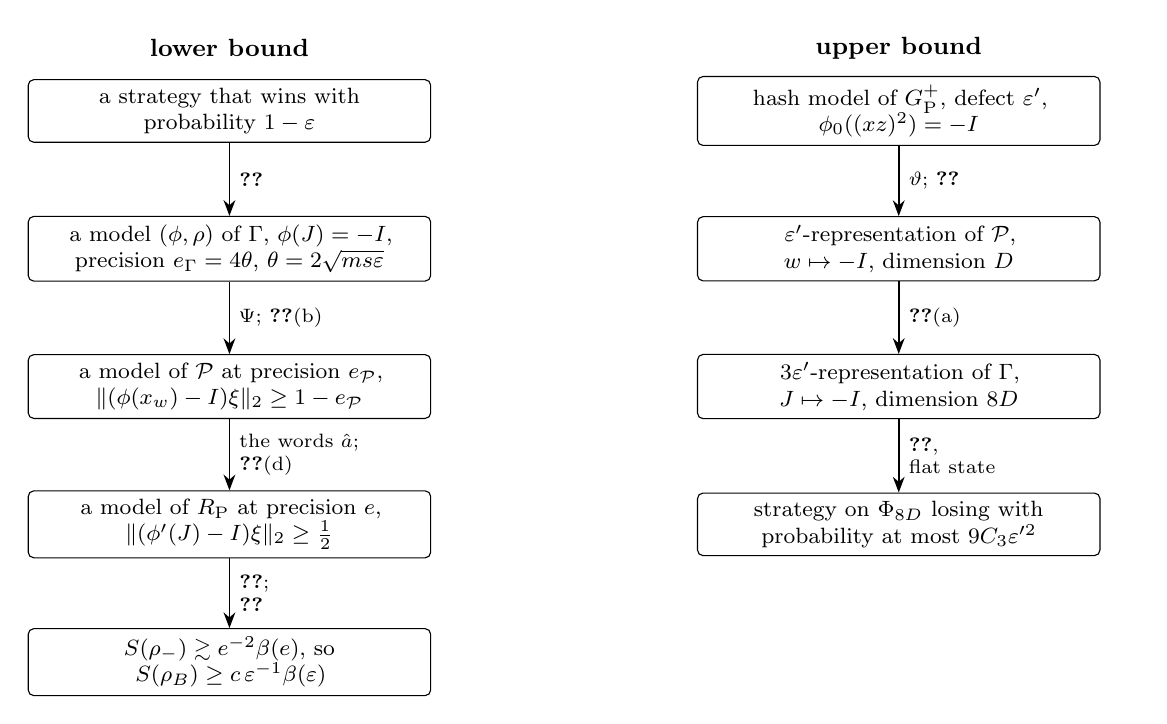
\begin{tikzpicture}[
  st/.style={draw,rounded corners=2pt,align=flush center,font=\footnotesize,text width=4.9cm,inner sep=3pt},
  ar/.style={-{Stealth[length=2mm]},semithick},
  lb/.style={font=\scriptsize,align=flush left,anchor=west,text width=2.8cm}]
\node[font=\small\bfseries] at (0,0.8) {lower bound};
\node[st] (l1) at (0,0) {a strategy that wins with\\ probability $1-\eps$};
\node[st] (l2) at (0,-1.75) {a model $(\phi,\rho)$ of $\Gamma$, $\phi(J)=-I$,\\ precision $e_\Gamma=4\theta$, $\theta=2\sqrt{ms\eps}$};
\node[st] (l3) at (0,-3.5) {a model of $\Pres$ at precision $e_\Pres$,\\ $\hs{(\phi(x_w)-I)\xi}\ge1-e_\Pres$};
\node[st] (l4) at (0,-5.25) {a model of $\RP$ at precision $e$,\\ $\hs{(\phi'(J)-I)\xi}\ge\frac12$};
\node[st] (l5) at (0,-7.0) {$S(\rho_-)\gtrsim e^{-2}\bfun(e)$, so\\ $S(\rho_B)\ge c\,\eps^{-1}\bfun(\eps)$};
\draw[ar] (l1)--node[lb,right]{\cref{thm:transfer}}(l2);
\draw[ar] (l2)--node[lb,right]{$\Psi$; \cref{thm:embedding}(b)}(l3);
\draw[ar] (l3)--node[lb,right]{the words $\hat a$;\\ \cref{prop:presentation}(d)}(l4);
\draw[ar] (l4)--node[lb,right]{\cref{thm:sector};\\ \cref{lem:sector-entropy}}(l5);
\node[font=\small\bfseries] at (8.5,0.8) {upper bound};
\node[st] (u1) at (8.5,0) {hash model of $\GPp$, defect $\eps'$,\\ $\phi_0((xz)^2)=-I$};
\node[st] (u2) at (8.5,-1.75) {$\eps'$-representation of $\Pres$,\\ $w\mapsto-I$, dimension $D$};
\node[st] (u3) at (8.5,-3.5) {$3\eps'$-representation of $\Gamma$,\\ $J\mapsto-I$, dimension $8D$};
\node[st] (u4) at (8.5,-5.25) {strategy on $\Phi_{8D}$ losing with\\ probability at most $9C_3\eps'^2$};
\draw[ar] (u1)--node[lb,right]{$\vartheta$; \cref{game:models}}(u2);
\draw[ar] (u2)--node[lb,right]{\cref{thm:embedding}(a)}(u3);
\draw[ar] (u3)--node[lb,right]{\cref{thm:return},\\ flat state}(u4);
\end{tikzpicture}
\caption{The two directions of the proof of Theorem~A. Here $e_\Pres=C_\Psi e_\Gamma$ and $e=36780\,e_\Pres$; on the right,
$\eps'=\frac13\sqrt{\eps/C_3}$ with the constant $C_3<788.2$ of \cref{thm:return}.}
\label{game:fig-map}
\end{figure}

\subsection{Proof of the lower bound}

Throughout, $m=1687$ and $s=3$; the default distribution has $\pi_{\min}=1/(ms)$. Let $\Psi$, $x_{j_0}$ and $A_0=42$ be as in
\cref{lem:gadget} and \cref{rem:A0}, and $C_\Psi=A_0(8A_0+17)=14826$ as in \cref{thm:embedding}. Put
\[
C_*=294240\,\sqrt{ms}\;C_\Psi<3.11\cdot10^{11},\qquad c_*=\frac{c_1}{512\,C_*^2}>4.9\cdot10^{-34},\qquad c_1=\frac1{4.1\cdot10^7},
\]
where $c_1$ is the constant of \cref{thm:sector}. We prove (b) with $c_*$ in place of $c$, which is stronger, and for every
$\eps_0\in(0,\frac14]$ such that, for $0<\eps\le\eps_0$,
\begin{equation}\label{game:eps0}
C_*\sqrt\eps\le2^{-1072}\qquad\text{and}\qquad c_*\,\eps^{-1}\bfun(\eps)\ge1 ;
\end{equation}
such an $\eps_0$ exists because $\eps^{-1}\bfun(\eps)\to\infty$ as $\eps\to0$. The value $\eps_0=2^{-5500}$ of \cref{thm:main} qualifies.
Write $L=\log(1/\eps)\ge5500$. The first condition says $L\ge2144+2\log C_*$, and $2144+2\log C_*<2221$. The second says
$L-4(24+\log L)^2\ge\log(1/c_*)$, where $\log(1/c_*)<111$. Its left side is increasing for $L\ge5500$ and exceeds $190$ at $L=5500$.

\begin{proof}[Proof of \cref{thm:main}(b)]
Let $0<\eps\le\eps_0$, fix a strategy that wins with probability at least $1-\eps$, and put $\theta=2\sqrt{\eps/\pi_{\min}}=2\sqrt{ms\eps}$.

\emph{Step 1: the transfer.} By \cref{thm:transfer} there are a homomorphism $\phi:F(x_1,\dots,x_n,J)\to\U(r)$, where $r$ is the Schmidt
rank of the state, and a density matrix $\rho$ of full rank on $\C^r$, Bob's reduced density matrix restricted to its support, such that,
with $\xi=\rho^{1/2}$, $\phi(J)=-I$, every relator $R'$ of $\Gamma$ has $\hs{(\phi(R')-I)\xi}\le\max(s,4)\theta=4\theta$, and every $x_j$ has
$\hs{[\phi(x_j),\xi]}\le\sqrt2\theta$. Since $\phi(J)=-I$ commutes with $\xi$, $(\phi,\rho)$ is a state-weighted model of $\Gamma$
(\cref{def:model}) at precision $e_\Gamma=4\theta$.

\emph{Step 2: from $\Gamma$ to $\Pres$.} By \cref{thm:embedding}(b), $(\phi_\Pres,\rho)$ with $\phi_\Pres=\phi\circ\Psi$ is a state-weighted model
of $\Pres$ at precision $e_\Pres=C_\Psi e_\Gamma$, and $W=\phi_\Pres(w)=\phi(x_w)$ satisfies
\[
\hs{(W-I)\xi}\ \ge\ 1-e_\Pres .
\]

\emph{Step 3: from $\Pres$ to $\RP$.} Put $\phi'(a)=\phi_\Pres(\hat a)$ for $a\in\{p,q,t,d,x,z\}$, so that $\phi'(r)=\phi_\Pres(\hat r)$ for every
word $r$ in these letters. Let $r\in\RP$. It has at most $22$ letters (\cref{def:RP}), so $\abs{\hat r}\le66$, and $\hat r$ has area at most
$60$ with respect to $R$ by \cref{prop:presentation}(d). The relators of $\Pres$ have length at most $4$, so by \cref{lem:conjugator-length}
the word $\hat r$ is freely equal to a product of at most $60$ conjugates of relators of $\Pres$ and their inverses, with conjugators of length
at most $66+60\cdot4=306$. By \cref{lem:calculus}(d), with \ref{prelim:S1} and \ref{prelim:S2} for $\Pres$ at precision $e_\Pres$,
\[
\hs{(\phi'(r)-I)\xi}\ \le\ 60\,(1+2\cdot306)\,e_\Pres\ =\ 36780\,e_\Pres .
\]
The same holds for the word $xzxz\,w^{-1}$, which has $5$ letters and area at most $60$. Each $\hat a$ has at most $3$ letters, so
$\hs{[\phi'(a),\xi]}\le3e_\Pres$ by \cref{lem:calculus}(a). Put
\[
e=36780\,e_\Pres=147120\,C_\Psi\,\theta=C_*\sqrt\eps .
\]
Then $(\phi',\rho)$ satisfies conditions (i) and (ii) of \cref{thm:sector} at precision $e$, and $e\le2^{-1072}$ by~\eqref{game:eps0}.

\emph{Step 4: visibility.} Here $J$ denotes the word $xzxz$, so $\phi'(J)=\phi_\Pres(xzxz)$ and $\phi'(J)W^*=\phi_\Pres(xzxz\,w^{-1})$.
Since $\phi'(J)-W=(\phi'(J)W^*-I)W$ and $W\xi=\xi W+[W,\xi]$,
\[
\hs{(\phi'(J)-W)\xi}\ \le\ \hs{(\phi'(J)W^*-I)\xi}+2\hs{[W,\xi]}\ \le\ e+2e_\Pres ,
\]
using Step~3 and \ref{prelim:S2} for the generator $w$. With Step~2 and $3e_\Pres\le e\le\frac14$,
\[
\hs{(\phi'(J)-I)\xi}\ \ge\ \hs{(W-I)\xi}-\hs{(\phi'(J)-W)\xi}\ \ge\ 1-e-3e_\Pres\ \ge\ \tfrac12 .
\]

\emph{Step 5: the sector.} By Steps~3 and~4, \cref{thm:sector} applies with $\Delta=\frac12$, since $e\le2^{-1072}=2^{-1071}\Delta$. Let
$J'=\mathrm r(\phi'(J))$ be the rounding of \cref{lem:rounding}, $P_-=\frac12(I-J')$, $p_-=\Tr(P_-\rho)$, and $\rho_-$ the sector state of
\cref{lem:sector-state} for $J'$. By \cref{thm:sector}, $p_-\ge\Delta^2/16=\frac1{64}$ and
\[
S(\rho_-)\ \ge\ \tfrac{c_1}4\,e^{-2}\,\bfun(e)\ \ge\ \frac{c_1}{4C_*^2}\,\eps^{-1}\bfun(\eps),
\]
because $e^{-2}=C_*^{-2}\eps^{-1}$, and $\eps\le\sqrt\eps\le e<\frac12$ (as $C_*\ge1$) with $\bfun$ nondecreasing on $(0,\frac12)$.

\emph{Step 6: back to $\rho$.} By \cref{lem:sector-entropy}, since $h\le1$,
\[
S(\rho)\ \ge\ p_-\,S(\rho_-)-1\ \ge\ \frac{c_1}{256\,C_*^2}\,\eps^{-1}\bfun(\eps)-1\ =\ 2c_*\,\eps^{-1}\bfun(\eps)-1\ \ge\ c_*\,\eps^{-1}\bfun(\eps),
\]
the last step by~\eqref{game:eps0}. Finally $\rho$ and $\rho_B$ have the same nonzero eigenvalues, so
$\log\rank\rho_B=\log\rank\rho\ge S(\rho)=S(\rho_B)$.
\end{proof}

The proof uses the strategy only through \cref{thm:transfer}, and the state only through \ref{prelim:S1} and \ref{prelim:S2}; no spectral
projection of $\rho$ is taken. Since $\omq(G)=1$ by (a), a strategy on $\C^d\otimes\C^d$ that wins with probability at least
$\omq(G)-\eps$ has Schmidt rank at most $d$, and (b) applies to it; so $\log\Ent(G,\eps)\ge c\,\eps^{-1}\bfun(\eps)$ for $0<\eps\le\eps_0$.

\begin{corollary}[Entanglement of formation]\label{cor:main-EF}
With $c$ and $\eps_0$ as in \cref{thm:main}(b), let $0<\eps\le\eps_0/2$. Every mixed state $\sigma$ on $H_A\otimes H_B$ and measurements
that win $G$ with probability at least $1-\eps$ satisfy
\[
E_F(\sigma)\ \ge\ \tfrac c4\,\eps^{-1}\bfun(\eps).
\]
\end{corollary}

\begin{proof}
Let $\sigma=\sum_jp_j\lvert\psi_j\rangle\langle\psi_j\rvert$ with $p_j>0$ and unit vectors $\psi_j$, and let $\ell_j$ be the losing
probability of the pure strategy that uses $\psi_j$ with the given measurements. The losing probability is linear in the state, so
$\sum_jp_j\ell_j\le\eps$, and the components with $\ell_j>2\eps$ carry total weight less than $\frac12$. Each component with $\ell_j\le2\eps$
is a strategy that wins with probability at least $1-2\eps$, with $2\eps\le\eps_0$, so by \cref{thm:main}(b) and the monotonicity of
$\bfun$,
\[
S\bigl(\Tr_A\lvert\psi_j\rangle\langle\psi_j\rvert\bigr)\ \ge\ c\,(2\eps)^{-1}\bfun(2\eps)\ \ge\ \tfrac c2\,\eps^{-1}\bfun(\eps).
\]
These components carry weight at least $\frac12$, so $\sum_jp_jS(\Tr_A\lvert\psi_j\rangle\langle\psi_j\rvert)\ge\frac c4\eps^{-1}\bfun(\eps)$.
The infimum over decompositions is $E_F(\sigma)$ (\cref{def:entanglement}).
\end{proof}

\subsection{Proof of the upper bound and of value one}

\begin{proof}[Proof of \cref{thm:main}(d) and (a)]
Let $C_3<788.2$ be the constant $C_s$ of \cref{thm:return} for $s=3$. Let $0<\eps\le\frac12$ and put $\eps'=\frac13\sqrt{\eps/C_3}\le1$.

\emph{Step 1: a representation of $\Pres$.} By \cref{game:models} there is an $\eps'$-representation of $\Pres$ with $w\mapsto-I$ in a
dimension $D$ with $\log_2D\le400\cdot44^2\,\eps'^{-2}\log_2(88/\eps')$.

\emph{Step 2: a representation of $\Gamma$.} By \cref{thm:embedding}(a) there is a $3\eps'$-representation $\phi_\Gamma$ of $\Gamma$ on
$\C^{8D}$ with $\phi_\Gamma(J)=-I$.

\emph{Step 3: a maximally entangled strategy.} Let $\rho=I/(8D)$ be the flat state. Then $\hs{Y\xi}=\fn{Y}$ for every operator $Y$, all state
commutators vanish, and $\phi_\Gamma(J)+I=0$, so $(\phi_\Gamma,\rho)$ is a model of $(\Gamma,J)$ at precision $3\eps'$
(\cref{def:model}). By \cref{thm:return}, the strategy built there on the canonical purification of $\rho$, which is the maximally
entangled state $\Phi_{8D}$, has local dimension $8D$ and loses every question pair, hence a random one, with probability at most
$C_3(3\eps')^2=\eps$.

\emph{Step 4: the count.} Since $\eps'^{-2}=9C_3\eps^{-1}$ and $88/\eps'=264\sqrt{C_3/\eps}$,
\[
\log_2(8D)\ \le\ 3+400\cdot44^2\cdot9\,C_3\,\eps^{-1}\Bigl(\log_2\bigl(264\sqrt{C_3}\bigr)+\tfrac12\log_2(1/\eps)\Bigr).
\]
Here $400\cdot44^2\cdot9\,C_3<5.50\cdot10^9$ and $\log_2(264\sqrt{C_3})<12.86$, and for $\eps\le\frac12$ we have $\log_2(1/\eps)\ge1$ and
$3\le\frac32\eps^{-1}\log_2(1/\eps)$. So $\log_2(8D)\le7.4\cdot10^{10}\,\eps^{-1}\log_2(1/\eps)$. Since $2^y\le e^y$ for $y\ge0$, the strategy
of Step~3 shows $\Entme(G,\eps)\le\exp(C\eps^{-1}\log(1/\eps))$ with $C=7.4\cdot10^{10}$, once we know $\omq(G)=1$.

\emph{Step 5: value one.} Step~3 gives, for every $0<\eps\le\frac12$, a strategy that wins with probability at least $1-\eps$. So
$\omq(G)=1$, which completes (d). Suppose a strategy on finite-dimensional spaces won with probability one. It would win with probability at
least $1-\eps$ for every $\eps$, so by (b) its reduced density matrix would satisfy $\log\rank\rho_B\ge c\,\eps^{-1}\bfun(\eps)$ for every
$0<\eps\le\eps_0$. The right side is unbounded as $\eps\to0$, while $\rank\rho_B\le\dim H_B$. So there is no such strategy. By
\cite[Thm.~3.2]{Slo19}, a linear system game has a perfect strategy on a tensor product of Hilbert spaces of arbitrary dimension if and only
if it has one on finite-dimensional spaces; so there is none of that kind either.
\end{proof}

\begin{proof}[Proof of the last sentence of \cref{thm:main}]
For $0<\eps\le\eps_0$, the paragraph after the proof of (b), $\Ent\le\Entme$ and (d) give
\[
c\,\eps^{-1}\bfun(\eps)\ \le\ \log\Ent(G,\eps)\ \le\ \log\Entme(G,\eps)\ \le\ C\log_2(e)\,\eps^{-1}\log(1/\eps).
\]
Since $\bfun(\eps)=\eps^{o(1)}$ and $\log(1/\eps)=\eps^{-o(1)}$, both logarithms are $\eps^{-1+o(1)}$.
\end{proof}

\subsection{Remarks}

\begin{remark}[The size of the game]\label{rem:game-size}
The four steps of \cref{lem:gadget}, applied to $\Pres$, give the following counts, which the generating program and the independent
checker of \cref{app:cert} both reproduce. Step~1 adds $12$ involutions ($f$, $v$, and one $Z_{bc}$ for each of the $10$ triples of $C_1$)
and $20$ conjugacy relations to the $76$ of $\Pres$. Step~2 adds the involutions $t^*$, $u$, the linear set $\{w,u\}$ and one conjugacy
relation; this leaves $N=40$ generators besides $J$ and $97$ conjugacy relations. Step~3 adds $3N+1+2\cdot97=315$ involutions and
$2N+2\cdot97=274$ linear sets, and turns the $97$ conjugacy relations into $N+2\cdot97=234$ nice ones. Step~4 replaces each nice relation
by $6$ equations in $7$ new variables. So $8+1+274=283$ equations come from linear sets and $6\cdot234=1404$ from gadgets, $1687$ in all,
in $26+12+2+315+1638=1993$ variables. All equations have three variables except $x_w+x_u=1$, which has two and is the only inhomogeneous
one. Gaussian elimination shows that $Ax=b$ has no solution over $\F_2$ ($A$ has rank $1512$), as it must, since $J$ is a commutator in
$\Gamma$: no deterministic strategy wins with certainty. A program independent of the generator also evaluates every relator of $\Gamma$ in
the representations $\gamma,\gamma_1,\gamma_2$ of the proof of \cref{lem:gadget}, built from the exact model of $\GPp$ with its central
involution $J$ in place of $-1$, and finds a homomorphism $\Gamma\to\GPp\wr\Sym(8)$ in which $J\ne1$ (\cref{cert:what}). None of this is used
in the proof of \cref{thm:main}, which needs only that $(A,b)$ is the output of \cref{lem:gadget}.
\end{remark}

\begin{remark}[The constants]\label{game:constants}
Only the constants $c$ and $\eps_0$ depend on the area constant $A_0=42$ of \cref{rem:A0}, and they are astronomically small: already
the precision condition $e\le2^{-1071}\Delta$ of the sector theorem forces $\eps_0<2^{-2144}$, and the factor $\bfun(\eps)$ pushes the
admissible $\eps_0$ down to about $2^{-5420}$. The constant $C$ of (d) is explicit, and
improving it is a matter of the hash models (the factor $400\,\ell_E^2$) and of the constant of \cref{thm:return}. The bounds (b) and (d) have
the same power of $\eps$; only the factors $\bfun(\eps)$ and $\log(1/\eps)$ separate them.
\end{remark}

\begin{remark}[Under the polynomial Dehn bound]\label{game:poly}
If the polynomial bound~\ref{H-poly} on the Dehn function of $H_3$ is used, \cref{rem:sector-poly} replaces the factor
$2^{-4(24+\log\log(1/e))^2}$ of \cref{thm:sector} by a constant multiple of $(\log(1/e))^{-4\kappa}$, for $e\le e_0\Delta$. The proof above
then gives \cref{thm:main}(b),(c) and \cref{cor:main-EF} with $\bfun(\eps)$ replaced by $(\log(1/\eps))^{-4\kappa}$, with new constants
$c,\eps_0$, since $e\ge\eps$ gives $(\log(1/e))^{-4\kappa}\ge(\log(1/\eps))^{-4\kappa}$.
\end{remark}

%======================================================================
\section{Two sharp rates}\label{sec:rates}
%======================================================================

The state-weighted method of \cref{sec:state,sec:count,sec:transfer} is not specific to lamp groups. This section applies it to two games
for which the earlier lower bounds lose a power of $\eps$ on the way from the strategy to a count. For the XOR games CHSH$(n)$ the qubit count of \cref{thm:count}, applied once in the reduced state
of the players, gives the ebit cost $\Theta(\min(n,1/\eps))$ (Theorem~E, \cref{sec:rates-chsh}). For the linear system game of Slofstra
and Vidick, a transport argument for spectral measures in one state gives the profile $\Theta(1/\eps)$ of its group and, through
\cref{thm:transfer}, the local dimension $\Theta(\eps^{-1/2})$ (Theorem~F, \cref{sec:rates-sv}). In both cases the new lower bound meets an
upper bound of the same order: for CHSH$(n)$ a known one, and for the game of Slofstra and Vidick theirs, through a lift that keeps the
distinguished involution balanced (\cref{lem:sv-lift}).

\subsection{The CHSH\texorpdfstring{$(n)$}{(n)} games}\label{sec:rates-chsh}

The XOR games CHSH$(n)$ of Slofstra~\cite{Slo11} force $n$ pairwise anticommuting observables on one side. A strategy within a factor
$1-\eps$ of the optimal bias pays a CHSH deficit for each of the $\binom n2$ pairs, and these deficits add up to $O(n^2\eps)$. From triples
of anticommuting observables one builds $\Theta(n)$ approximate qubits~\cite{OV18}, and \cref{thm:count} charges each of them only the sum
of the squares of its pair errors, which is $O(n\eps)$. So a constant fraction of the $n/3$ qubits survives as long as $n\eps$ is small.

\begin{definition}[CHSH$(n)$; \cite{Slo11}, {\cite[Section~2.3]{OV18}}]\label{def:chsh}
In CHSH$(n)$, $n\ge2$, the referee picks $i<j$ uniformly, sends Alice $i$ or $j$ and Bob $(i,j)$ or $(j,i)$, independently and uniformly,
and accepts if and only if $a\oplus b=1$ when Alice received $j$ and Bob $(j,i)$, and $a\oplus b=0$ otherwise. A strategy is a unit vector
$\psi\in H_A\otimes H_B$, with $H_A,H_B$ finite-dimensional, together with binary observables (Hermitian contractions) $A_k$ for Alice,
$k\in[n]$, and $B_{ij}$ for Bob, $i\ne j$. Its \emph{bias}, the probability of winning minus that of losing, is
\[
\operatorname{bias}=\frac1{2n(n-1)}\sum_{i<j}C_{ij},\qquad C_{ij}=\ip{\psi}{(A_i\otimes(B_{ij}+B_{ji}))\psi}+\ip{\psi}{(A_j\otimes(B_{ij}-B_{ji}))\psi}.
\]
The optimal bias is $\operatorname{bias}^*=\sqrt2/2$, and a strategy is \emph{$\eps$-optimal} if $\operatorname{bias}\ge(1-\eps)\operatorname{bias}^*$.
\end{definition}

Ostrev and Vidick measure the bias by its absolute value; replacing every $A_k$ by $-A_k$ changes its sign and nothing else, so we may take
it nonnegative. The next lemma is the robust form of Tsirelson's bound for one pair, with every error measured in Alice's reduced state.

\begin{lemma}[One pair]\label{lem:one-pair}
Let $A,A'$ be involutions on $H_A$, $B,B'$ involutions on $H_B$, $\psi\in H_A\otimes H_B$ a unit vector and $\xi_A=\rho_A^{1/2}$. Put
$T_0=(B+B')/\sqrt2$, $T_1=(B-B')/\sqrt2$,
$C=\ip{\psi}{(A\otimes(B+B'))\psi}+\ip{\psi}{(A'\otimes(B-B'))\psi}$ and $\delta=2\sqrt2-C$. Then
\[
\delta=\frac1{\sqrt2}\Bigl(\lVert(A\otimes I-I\otimes T_0)\psi\rVert^2+\lVert(A'\otimes I-I\otimes T_1)\psi\rVert^2\Bigr).
\]
Consequently $\delta\ge0$, and
\[
\hs{\{A,A'\}\xi_A}^2\le33\,\delta,\qquad\hs{[A,\xi_A]}^2\le2\sqrt2\,\delta,\qquad\hs{[A',\xi_A]}^2\le2\sqrt2\,\delta.
\]
\end{lemma}

\begin{proof}
Write $\langle\cdot\rangle$ for the expectation in $\psi$. Since $A^2=I$, $\lVert(A\otimes I-I\otimes T_0)\psi\rVert^2=1+\langle
T_0^2\rangle-\sqrt2\langle A\otimes(B+B')\rangle$, and likewise for the second norm. As $T_0^2+T_1^2=B^2+B'^2=2I$, the sum of the two norms
is $4-\sqrt2\,C$, which is the identity. So both norms are at most $\tau=(\sqrt2\delta)^{1/2}$. Since $\{T_0,T_1\}=B^2-B'^2=0$ and
$\op{T_0},\op{T_1}\le\sqrt2$, and since $A\otimes I$ commutes with $I\otimes T_1$,
\[
(AA'\otimes I)\psi=(A\otimes I)(I\otimes T_1)\psi+(A\otimes I)\bigl((A'\otimes I)-(I\otimes T_1)\bigr)\psi=(I\otimes T_1T_0)\psi+\epsilon_1,
\]
with $\lVert\epsilon_1\rVert\le(1+\sqrt2)\tau$. In the same way $(A'A\otimes I)\psi=(I\otimes T_0T_1)\psi+\epsilon_2$ with
$\lVert\epsilon_2\rVert\le(1+\sqrt2)\tau$. Adding, and using \cref{lem:standard-form}(a) for Alice's side,
$\hs{\{A,A'\}\xi_A}\le2(1+\sqrt2)\tau$; and $4(1+\sqrt2)^2\sqrt2<33$. Finally \cref{lem:standard-form}(b), with the roles of the two
factors exchanged, gives Hermitian operators $\tilde T_0,\tilde T_1$ on $H_A$ with $\hs{A\xi_A-\xi_A\tilde T_0}$,
$\hs{A'\xi_A-\xi_A\tilde T_1}\le\tau$, and \cref{lem:consistency} gives the last two bounds.
\end{proof}

With all observables involutions, the lemma gives $C_{ij}\le2\sqrt2$, which is Tsirelson's bound~\cite{Cir80}, and hence
$\operatorname{bias}\le\operatorname{bias}^*$; the reduction to involutions in the next proof shows that this holds for all strategies.

\begin{theorem}[Ebits for CHSH$(n)$]\label{thm:chsh}
Let $n\ge3$ and $\eps>0$, and put $M=\lfloor\min(n,10^{-7}/\eps)/3\rfloor$. Every $\eps$-optimal strategy for CHSH$(n)$ satisfies
\[
S(\rho_A)\ \ge\ M/2 .
\]
In particular $S(\rho_A)\ge10^{-7}\min(n,1/\eps)/6-1/2$.
\end{theorem}

The proof selects $n'=3M$ questions whose pairwise CHSH deficits are small on average, splits them into $M$ triples, turns each triple
into one approximate Pauli pair as in~\cite{OV18}, and applies \cref{thm:count} to the $M$ pairs in Alice's reduced state. The pair errors
enter only through their squares, which add up to $O(n'^2\eps)$, that is, $O(n'\eps)$ per qubit.

\begin{proof}
If $M=0$ there is nothing to prove, so let $M\ge1$ and $n'=3M\le\min(n,10^{-7}/\eps)$.

\emph{Step 0: reductions.} With all other observables fixed, the bias is an affine function $\Tr(A_kN_k)+\mathrm{const}$ of Alice's
observable $A_k$, with $N_k$ Hermitian, so replacing $A_k$ by $\sgn(N_k)$ (with $\sgn(0)=1$) does not lower it; the same holds for Bob's
observables. Doing this for each observable in turn, we may assume that all observables are involutions; the state is unchanged. Let
$\delta_{ij}=2\sqrt2-C_{ij}\ge0$ (\cref{lem:one-pair}). From $\operatorname{bias}\ge(1-\eps)\sqrt2/2$,
\[
\sum_{i<j}\delta_{ij}\ \le\ 2\sqrt2\,\eps\binom n2 .
\]
Averaging over uniformly random $n'$-subsets of $[n]$, fix a subset $\mathcal N$ whose pair average
$\bar\delta=\binom{n'}2^{-1}\sum_{x<y\in\mathcal N}\delta_{xy}$ is at most $2\sqrt2\,\eps$. A fixed pair of $\mathcal N$ lies in a common block of a
uniformly random partition of $\mathcal N$ into $M$ triples with probability $2/(n'-1)$; fix a partition $\mathcal T_1,\dots,\mathcal T_M$
for which the sum of $\delta_{xy}$ over the $3M$ pairs inside the triples is at most $\frac2{n'-1}\binom{n'}2\bar\delta=n'\bar\delta$.

\emph{Step 1: pair errors.} Write $\xi=\rho_A^{1/2}$, $\eta_{xy}=\hs{\{A_x,A_y\}\xi}$ and $c_x=\hs{[A_x,\xi]}$. Applying \cref{lem:one-pair}
to the pair $\{x,y\}$, with $(A,A',B,B')=(A_x,A_y,B_{xy},B_{yx})$ for $x<y$,
\[
\eta_{xy}^2\le33\,\delta_{xy},\qquad c_x^2\le2\sqrt2\,\delta_{xy}\quad\text{for every }y\ne x.
\]
Choosing for each $x\in\mathcal N$ the partner $y\in\mathcal N$ with the least $\delta_{xy}$,
\[
\sum_{x\in\mathcal N}c_x^2\ \le\ 2\sqrt2\sum_{x\in\mathcal N}\frac1{n'-1}\sum_{y\in\mathcal N\setminus x}\delta_{xy}\ =\ 2\sqrt2\,n'\bar\delta .
\]

\emph{Step 2: one qubit from each triple.} The construction of pairs from triples is that of~\cite{OV18}. For $\mathcal T_k=\{a,b,c\}$,
labelled in any order, put $U_k=iA_aA_b$ and $W_k=iA_bA_c$, which are unitaries, and let $X_k=\mathrm r(U_k)$ and $Z_k=\mathrm r(W_k)$ be
their roundings (\cref{lem:rounding}). Since $U_k^2-I=-A_aA_b\{A_a,A_b\}$, we have $\hs{(U_k^2-I)\xi}=\eta_{ab}$, so
\[
\hs{(X_k-U_k)\xi}\le\eta_{ab},\qquad\hs{[X_k,\xi]}\le c_a+c_b+2\eta_{ab},
\]
and likewise for $Z_k$ with $(b,c)$ in place of $(a,b)$. Put $\lambda_k=\eta_{ab}+\eta_{bc}+\eta_{ac}+c_a+c_b+c_c$ and, for $k\ne l$,
$\mu_{kl}=\sum_{x\in\mathcal T_k,\,y\in\mathcal T_l}\eta_{xy}$. For distinct indices $b,c,b',c'$, and for one triple $\{a,b,c\}$, we have
the identities, which use only $A_x^2=I$,
\begin{align*}
A_bA_cA_{b'}A_{c'}-A_{b'}A_{c'}A_bA_c&=A_b\{A_c,A_{b'}\}A_{c'}-\{A_b,A_{b'}\}A_cA_{c'}\\
&\quad+A_{b'}A_b\{A_c,A_{c'}\}-A_{b'}\{A_b,A_{c'}\}A_c,\\
\{U_k,W_k\}&=-A_b\{A_a,A_c\}A_b+\{A_a,A_b\}A_cA_b-A_aA_b\{A_b,A_c\}.
\end{align*}
Apply them to $\xi$ and move the trailing observables to the right of $\xi$, at cost $2c_x$ for each, the anticommutators having norm at
most $2$. For $k\ne l$ this gives
\[
\hs{[W_k,W_l]\xi},\ \hs{[U_k,W_l]\xi}\ \le\ \mu_{kl}+4\lambda_k+4\lambda_l,\qquad\hs{\{U_k,W_k\}\xi}\le4\lambda_k .
\]
\Cref{lem:calculus}(e), with the primed operators the unitaries $U$ and $W$, whose state commutators are at most $\lambda_k$, replaces
$U,W$ by $X,Z$: for $k\ne l$,
\begin{gather*}
\hs{[Z_k,Z_l]\xi},\ \hs{[X_k,Z_l]\xi}\le\mu_{kl}+8\lambda_k+8\lambda_l,\\
\hs{\{X_k,Z_k\}\xi}\le12\lambda_k,\qquad\hs{[X_k,\xi]},\ \hs{[Z_k,\xi]}\le2\lambda_k .
\end{gather*}

\emph{Step 3: counting.} Apply \cref{thm:count} to the $M$ pairs $(X_k,Z_k)$ in the state $\rho_A$. With
$c^X_k=\hs{[X_k,\xi]}$ and $c^Z_k=\hs{[Z_k,\xi]}$, its parts (i)--(iii) give numbers $a_k,b_k\ge0$ with
$a_k^2\le2\sum_{l>k}(\hs{[Z_k,Z_l]\xi}+c^Z_l)^2+2\sum_{l>k}(c^Z_l)^2$,
$b_k^2\le2(\hs{\{X_k,Z_k\}\xi}+c^Z_k)^2+2\sum_{l\ne k}(\hs{[X_k,Z_l]\xi}+c^Z_l)^2+2\sum_{l}(c^Z_l)^2$ and
\[
S(\rho_A)\ \ge\ \sum_{k=1}^M\Bigl[1-\frac{(b_k+c^X_k)^2}{2\ln2}-h\Bigl(\min\Bigl(\frac{(a_k+c^Z_k)^2}4,\frac12\Bigr)\Bigr)\Bigr].
\]
Put $\Sigma_\lambda=\sum_k\lambda_k^2$. By Step~2 and $(x+y+z)^2\le3(x^2+y^2+z^2)$,
\[
a_k^2\le6\sum_{l\ne k}\mu_{kl}^2+384M\lambda_k^2+608\,\Sigma_\lambda,\qquad b_k^2\le392\lambda_k^2+6\sum_{l\ne k}\mu_{kl}^2+384M\lambda_k^2+608\,\Sigma_\lambda .
\]
By $(x+y)^2\le2x^2+2y^2$, the monotonicity of $h$ on $[0,\frac12]$, and Jensen's inequality for the concave nondecreasing function
$t\mapsto h(\min(t,\frac12))$,
\[
S(\rho_A)\ \ge\ M-\frac{B}{\ln2}-M\,h\Bigl(\min\Bigl(\frac A{2M},\frac12\Bigr)\Bigr),\qquad A=\sum_k(a_k^2+4\lambda_k^2),\quad B=\sum_k(b_k^2+4\lambda_k^2).
\]
Now $\mu_{kl}^2\le9\sum_{x\in\mathcal T_k,y\in\mathcal T_l}\eta_{xy}^2$, so $\sum_{k\ne l}\mu_{kl}^2\le18\sum_{x<y\in\mathcal
N}\eta_{xy}^2\le594\binom{n'}2\bar\delta\le297\,n'^2\bar\delta$, and $\Sigma_\lambda\le6\bigl(\sum_{\rm internal}\eta_{xy}^2+\sum_{x\in\mathcal
N}c_x^2\bigr)\le6(33+2\sqrt2)\,n'\bar\delta\le215\,n'\bar\delta$, where the internal pairs are those inside the triples. Hence, with
$M\ge1$ and $M=n'/3$,
\[
A\le6\cdot297\,n'^2\bar\delta+996\,M\Sigma_\lambda\le73162\,n'^2\bar\delta,\qquad B\le6\cdot297\,n'^2\bar\delta+1388\,M\Sigma_\lambda\le101256\,n'^2\bar\delta .
\]
With $\bar\delta\le2\sqrt2\,\eps$ this gives
\[
S(\rho_A)\ \ge\ M\Bigl[1-1.24\cdot10^6\,n'\eps-h\bigl(\min(3.11\cdot10^5\,n'\eps,\tfrac12)\bigr)\Bigr].
\]
Since $n'\eps\le10^{-7}$, the bracket is at least $1-0.124-h(0.0311)>0.67$, so $S(\rho_A)\ge M/2$. Finally
$M\ge\min(n,10^{-7}/\eps)/3-1\ge10^{-7}\min(n,1/\eps)/3-1$.
\end{proof}

\begin{corollary}[The ebit cost of CHSH$(n)$]\label{cor:chsh-ebits}
Let $S_{\min}(n,\eps)$ be the least entanglement entropy $S(\rho_A)$ of an $\eps$-optimal strategy for CHSH$(n)$. For $n\ge3$ and
$0<\eps\le1$,
\[
\frac{10^{-7}}6\min(n,1/\eps)-\frac12\ \le\ S_{\min}(n,\eps)\ \le\ \min\bigl(\lfloor n/2\rfloor,\lceil1/\eps\rceil\bigr).
\]
So $S_{\min}(n,\eps)=\Theta(\min(n,1/\eps))$ as $\min(n,1/\eps)\to\infty$.
\end{corollary}

\begin{proof}
The lower bound is \cref{thm:chsh}. For the upper bound $\lceil1/\eps\rceil$, every XOR game has an $\eps$-optimal strategy on a maximally
entangled state of local dimension $2^{\lceil1/\eps\rceil}$~\cite[Theorem~2]{OV18}. For the upper bound $\lfloor n/2\rfloor$, let
$m=\lfloor n/2\rfloor$; the Jordan--Wigner construction gives $2m+1\ge n$ pairwise anticommuting involutions $A_1,\dots,A_n$ on
$(\C^2)^{\otimes m}$. On the maximally entangled state $\Phi$ of local dimension $2^m$, for which $\ip{\Phi}{(Y\otimes Z^T)\Phi}=2^{-m}\Tr(YZ)$,
let Bob use $B_{ij}=((A_i+A_j)/\sqrt2)^T$ and $B_{ji}=((A_i-A_j)/\sqrt2)^T$ for $i<j$, which are involutions. Then
$B_{ij}+B_{ji}=\sqrt2A_i^T$ and $B_{ij}-B_{ji}=\sqrt2A_j^T$, so $C_{ij}=2\sqrt2$ for every pair and
$\operatorname{bias}=\operatorname{bias}^*$, with $m$ ebits~\cite{Slo11,OV18}.
\end{proof}

The entropy bound does not use purity in an essential way: shared randomness cannot lower the entanglement of formation.

\begin{corollary}[Entanglement of formation]\label{cor:chsh-ef}
Let $\sigma$ be a state on $H_A\otimes H_B$ and let binary observables for CHSH$(n)$, $n\ge3$, achieve bias at least
$(1-\eps)\operatorname{bias}^*$ on $\sigma$. Then
\[
E_F(\sigma)\ \ge\ \frac14\Bigl\lfloor\frac13\min\Bigl(n,\frac{10^{-7}}{2\eps}\Bigr)\Bigr\rfloor .
\]
\end{corollary}

\begin{proof}
Let $\sigma=\sum_jp_j\lvert\psi_j\rangle\langle\psi_j\rvert$ be any decomposition into pure states. The bias is linear in the state, so
$\operatorname{bias}(\sigma)=\sum_jp_j\operatorname{bias}(\psi_j)$ with the same observables, and
$\operatorname{bias}(\psi_j)\le\operatorname{bias}^*$. Put $\eps_j=1-\operatorname{bias}(\psi_j)/\operatorname{bias}^*\ge0$; then
$\sum_jp_j\eps_j\le\eps$, so the components with $\eps_j\le2\eps$ have total weight at least $\frac12$. Each of them is a $2\eps$-optimal
pure strategy, so its reduced state on $H_A$ has entropy at least half the floor in the statement, by \cref{thm:chsh}. Averaging over $j$,
with entropy $\ge0$ for the other components, and taking the infimum over decompositions gives the claim.
\end{proof}

The strategies of \cref{cor:chsh-ebits} use pure states, for which $E_F$ is the entanglement entropy, so the entanglement of formation
needed is also $\Theta(\min(n,1/\eps))$. \emph{Theorem~E is \cref{thm:chsh} with \cref{cor:chsh-ebits,cor:chsh-ef}.}

\begin{remark}\label{rates:rem-chsh}
The rate is linear in $1/\eps$, which~\cite[Theorem~2]{OV18} shows is optimal; the lower bound of~\cite[Theorem~1]{OV18} is
$\Omega(\eps^{-1/5})$, with the same question sets of sizes $n$ and $n(n-1)$. The argument of~\cite{OV18} also builds about $n/3$ pairs from
triples, but converts approximate anticommutation into a qubit count with polynomial losses at each step. Here every error stays in the
state-weighted $\ell^2$ norm, and \cref{thm:count} is applied once. The threshold $n\eps\approx1$ at which the count stops is the scale at
which the maximally entangled strategy of~\cite[Theorem~2]{OV18}, with $\lceil1/\eps\rceil$ ebits, becomes cheaper than the exact strategy
with $\lfloor n/2\rfloor$.
\end{remark}

\subsection{The Slofstra--Vidick group and game}\label{sec:rates-sv}

Slofstra and Vidick built a linear system game $\Gsv$ with $C\eps^{-1/6}\le\Ent(\Gsv,\eps)\le C'\eps^{-1/2}$~\cite[Theorem~1.1]{SV18} from
the group~\cite[Proposition~3.2]{SV18}
\begin{equation}\label{eq:K}
K=\bigl\langle a,b,c,x,y\ \bigm|\ xyx^{-1}y^{-2},\ xcx^{-1}c^{-1},\ yay^{-1}b^{-1},\ yby^{-1}a^{-1},\ c^{-1}ab,\ a^2,\ b^2,\ c^2\bigr\rangle,
\end{equation}
in which $c$ is a central involution, and whose profile satisfies $C\eps^{-2/3}\le\hlp_K(c;\delta,\eps)\le C'/\eps$. We show that both
lower exponents are the upper ones: $\hlp_K(c;\delta,\eps)=\Theta(1/\eps)$ (\cref{cor:K-profile}) and $\Ent(\Gsv,\eps)=\Theta(\eps^{-1/2})$
(\cref{thm:sv-game}).

The picture is as follows. Let $\mu$ be the spectral measure of $\phi(y)$ in the state. The relation $xyx^{-1}=y^2$ makes $\mu$ nearly
invariant under the doubling map $\vartheta\mapsto2\vartheta$ of the circle, and, where $c$ acts as $-1$, the relations $yay^{-1}=b$ and
$c=ab$ make it nearly invariant under the half-turn $\vartheta\mapsto\vartheta+\pi$. Averaging over the two inverse branches of the
doubling map contracts the Wasserstein distance by a factor $2$, so a measure that is nearly invariant under both maps is close to Haar
measure (\cref{prop:K-W1}), while a measure with $d$ atoms is at distance at least $\pi/(2d)$ from it. All quantities are measured in
one state; the
Wasserstein-$1$ distance, rather than a quadratic one, is what makes a change of state cost only a linear error.

\subsubsection*{Measures on the circle}

Let $\T=\R/2\pi\Z$ with the geodesic distance $d(\vartheta,\vartheta')\in[0,\pi]$, and let $\mathsf h$ be the normalized Haar measure. For
probability measures $\mu,\nu$ on $\T$ put
\[
W_1(\mu,\nu)=\sup\Bigl\{\int f\,d\mu-\int f\,d\nu\ :\ f:\T\to\R\text{ is $1$-Lipschitz}\Bigr\}.
\]
By Kantorovich--Rubinstein duality~\cite[Chapter~5]{Vil09} this is the least mean distance of a coupling of $\mu$ and $\nu$; we use only
the triangle inequality and the elementary bound $W_1(\mu,\nu)\le\int d\,d\gamma$ for every coupling $\gamma$ of $\mu$ and $\nu$, which
holds because $\int f\,d\mu-\int f\,d\nu=\int(f(\vartheta)-f(\vartheta'))\,d\gamma$. Let $\mathsf D(\vartheta)=2\vartheta$ and
$\mathsf S(\vartheta)=\vartheta+\pi$, with push-forwards $\mathsf D_*$, $\mathsf S_*$. The two square roots of $e^{i\vartheta}$ have angles
$\vartheta/2$ and $\vartheta/2+\pi$, a set that does not depend on the representative of $\vartheta$. Let $\mathsf P$ replace each point by
the uniform measure on its two square roots: $\int f\,d(\mathsf P\mu)=\int\mathsf P^*f\,d\mu$ with
$\mathsf P^*f(\vartheta)=\frac12\bigl(f(\vartheta/2)+f(\vartheta/2+\pi)\bigr)$.

\begin{lemma}[Doubling and half-turn]\label{lem:circle}
For probability measures $\mu,\nu$ on $\T$:
\begin{enumerate}[label=(\alph*),itemsep=1pt]
\item $\mathsf P\mathsf h=\mathsf h$ and $\mathsf P(\mathsf D_*\mu)=\frac12(\mu+\mathsf S_*\mu)$;
\item $W_1(\mathsf P\mu,\mathsf P\nu)\le\frac12W_1(\mu,\nu)$;
\item $W_1(\mu,\mathsf h)\le W_1(\mathsf D_*\mu,\mu)+W_1(\mathsf S_*\mu,\mu)$;
\item if $\mu$ is supported on at most $d$ points, then $W_1(\mu,\mathsf h)\ge\pi/(2d)$.
\end{enumerate}
\end{lemma}

\begin{proof}
(a) The maps $\vartheta\mapsto\vartheta/2$ and $\vartheta\mapsto\vartheta/2+\pi$, on a fundamental interval of length $2\pi$, carry $\mathsf h$ to
the uniform measures on two complementary half-circles, so $\int\mathsf P^*f\,d\mathsf h=\int f\,d\mathsf h$. The square roots of
$e^{2i\vartheta}$ are $\vartheta$ and $\vartheta+\pi$.

(b) Let $f$ be $1$-Lipschitz and $d(\vartheta,\vartheta')=t$. Choose real representatives with $\vartheta'=\vartheta+s$ and $\lvert
s\rvert=t\le\pi$. The roots $\vartheta/2$ and $(\vartheta+s)/2$, and the roots $\vartheta/2+\pi$ and $(\vartheta+s)/2+\pi$, are at distance at
most $\lvert s\rvert/2$, so $\lvert\mathsf P^*f(\vartheta)-\mathsf P^*f(\vartheta')\rvert\le t/2$. Thus $2\mathsf P^*f$ is $1$-Lipschitz and
$\int f\,d(\mathsf P\mu-\mathsf P\nu)=\int\mathsf P^*f\,d(\mu-\nu)\le\frac12W_1(\mu,\nu)$.

(c) By the triangle inequality, (a) and (b),
\begin{align*}
W_1(\mu,\mathsf h)&\le W_1(\mu,\mathsf P\mathsf D_*\mu)+W_1(\mathsf P\mathsf D_*\mu,\mathsf P\mu)+W_1(\mathsf P\mu,\mathsf P\mathsf h)\\
&\le\tfrac12W_1(\mu,\mathsf S_*\mu)+\tfrac12W_1(\mathsf D_*\mu,\mu)+\tfrac12W_1(\mu,\mathsf h),
\end{align*}
where the first term was computed directly: $\int f\,d(\mu-\frac12(\mu+\mathsf S_*\mu))=\frac12\int f\,d(\mu-\mathsf S_*\mu)$. Since
$W_1(\mu,\mathsf h)\le\pi$ is finite, (c) follows.

(d) Let $k\le d$ be the number of points of $\supp\mu$. They cut $\T$ into $k$ arcs of lengths $l_1,\dots,l_k$ with $\sum_jl_j=2\pi$. The function
$f(\vartheta)=d(\vartheta,\supp\mu)$ is $1$-Lipschitz, $\int f\,d\mu=0$, and, by Cauchy--Schwarz,
\[
\int f\,d\mathsf h=\frac1{2\pi}\sum_j\int_0^{l_j}\min(t,l_j-t)\,dt=\sum_j\frac{l_j^2}{8\pi}\ \ge\ \frac{(2\pi)^2}{8\pi k}=\frac\pi{2k}. \qedhere
\]
\end{proof}

The operator $\mathsf P$ is the transfer operator of the doubling map, and (b) is an averaged form of the square-root lifting that Slofstra
and Vidick use in operator norm~\cite[Claims~3.6 and~3.7]{SV18}. Part~(d) needs no lower bound on the masses of the atoms.

For a unitary $Y$ and a density matrix $\rho$ on $\C^d$ let $\mu^\rho_Y$ be the \emph{spectral measure of $Y$ in $\rho$}, the probability
measure on $\T$ with $\int f\,d\mu^\rho_Y=\Tr(\rho f(Y))$, where $f(Y)$ applies $f$ to the angles of the eigenvalues. It is supported on
the angles of the at most $d$ eigenvalues of $Y$, and
\begin{equation}\label{eq:rates-spectral}
\mu^\rho_{Y^2}=\mathsf D_*\mu^\rho_Y,\qquad\mu^\rho_{-Y}=\mathsf S_*\mu^\rho_Y,\qquad\mu^\rho_{UYU^*}=\mu^{U^*\rho U}_Y\quad(U\text{ unitary}).
\end{equation}

\begin{lemma}[Coupling in one state]\label{lem:coupling}
Let $P,Q,Y,U$ be unitaries on $\C^d$ and $\xi=\rho^{1/2}$.
\begin{enumerate}[label=(\alph*),itemsep=1pt]
\item There is a coupling $\nu$ of $\mu^\rho_P$ and $\mu^\rho_Q$, viewed on the unit circle, with $\int\lvert z-z'\rvert^2\,d\nu(z,z')=\hs{P\xi-\xi
Q}^2$. Hence $W_1(\mu^\rho_P,\mu^\rho_Q)\le\frac\pi2\hs{P\xi-\xi Q}$.
\item $W_1(\mu^{U^*\rho U}_Y,\mu^\rho_Y)\le\pi\hs{[U,\xi]}$.
\end{enumerate}
\end{lemma}

\begin{proof}
(a) Let $P=\sum_iz_iE_i$ and $Q=\sum_jz'_jF_j$ be spectral decompositions with distinct eigenvalues, and
$\nu=\sum_{i,j}\hs{E_i\xi F_j}^2\,\delta_{(z_i,z'_j)}$. The operators $E_i\xi F_j$ are mutually orthogonal in the Hilbert--Schmidt inner
product. Since $\sum_jF_j=I$, $\sum_j\hs{E_i\xi F_j}^2=\hs{E_i\xi}^2=\Tr(E_i\rho)$, and likewise $\sum_i\hs{E_i\xi F_j}^2=\Tr(\rho F_j)$, so
$\nu$ couples $\mu^\rho_P$ and $\mu^\rho_Q$; and $\int\lvert z-z'\rvert^2d\nu=\hs{\sum_{i,j}(z_i-z'_j)E_i\xi F_j}^2=\hs{P\xi-\xi Q}^2$. The arc
length between two points of the unit circle is at most $\frac\pi2$ times their chordal distance, and $\int\lvert z-z'\rvert\,d\nu\le(\int\lvert
z-z'\rvert^2d\nu)^{1/2}$.

(b) Let $f$ be $1$-Lipschitz and $f_0=f-c_f$, with $c_f$ the midpoint of the range of $f$, so that $\lvert f_0\rvert\le\pi/2$, the diameter
of $\T$ being $\pi$. Both measures have mass one, so $\int f\,d(\mu^{U^*\rho U}_Y-\mu^\rho_Y)=\Tr\bigl((U^*\rho U-\rho)f_0(Y)\bigr)\le\frac\pi2\tn{U^*\rho
U-\rho}$, which is at most $\pi\hs{[U,\xi]}$ by \cref{lem:rotate}.
\end{proof}

The coupling in (a) is Connes' joint distribution trick~\cite[Lemma~1.2.6]{Con76}, in the form used in~\cite[Lemma~5.5]{SV18}; for
$\rho=I/d$ it gives the Hoffman--Wielandt inequality. Part~(b) is the reason for working with $W_1$: a change of state by a unitary costs
the state commutator linearly.

\subsubsection*{The profile of \texorpdfstring{$K$}{K}}

\begin{theorem}[The profile of $c$ in a state]\label{thm:K-profile}
Let $\phi$ assign unitaries $A,B,C,X,Y$ on $\C^d$ to $a,b,c,x,y$, and let $\rho$ be a density matrix on $\C^d$ with $\xi=\rho^{1/2}$.
Suppose that, for some $e>0$,
\begin{enumerate}[label=(\roman*),itemsep=1pt]
\item every relator $r$ in~\eqref{eq:K} has $\hs{(\phi(r)-I)\xi}\le e$;
\item $\hs{[\phi(s),\xi]}\le e$ for $s\in\{a,b,c,x,y\}$;
\item $\hs{(C+I)\xi}\le e$.
\end{enumerate}
Then $d\ge1/(29e)$. In the notation of \cref{def:state-profile}, $\hlps_K(c;e)\ge1/(29e)$.
\end{theorem}

The two relations are read off as near-invariances of $\mu=\mu^\rho_Y$, each up to a coupling in the state (\cref{lem:coupling}(a)) and a
change of state by a unitary (\cref{lem:coupling}(b)); \cref{lem:circle} then compares $\mu$ with Haar measure. That comparison does not
involve the dimension, and we state it on its own.

\begin{proposition}[The spectral measure of $y$ in a state]\label{prop:K-W1}
Under the hypotheses of \cref{thm:K-profile}, the spectral measure of $Y=\phi(y)$ in $\rho$ satisfies
\[
W_1(\mu^\rho_Y,\mathsf h)\ \le\ \frac{29\pi}2\,e .
\]
\end{proposition}

The bound uses all three hypotheses: the state commutators~(ii) pay for the changes of state in \cref{lem:coupling}(b), and~(iii), which
says that $c$ acts as $-1$ in the state, turns the relations $yay^{-1}=b$ and $c=ab$ into the half-turn.

\begin{proof}
Let $\mu=\mu^\rho_Y$, $\delta_{\mathsf D}=W_1(\mathsf D_*\mu,\mu)$ and $\delta_{\mathsf S}=W_1(\mathsf S_*\mu,\mu)$.

\emph{Doubling.} Put $P=Y^2$ and $Q=XYX^*$. The relator $r=xyx^{-1}y^{-2}$ has $\phi(r)=QP^*$, so $(Q-P)\xi=(\phi(r)-I)P\xi=(\phi(r)-I)\xi
P+(\phi(r)-I)[P,\xi]$, and $\hs{[P,\xi]}\le2e$; hence $\hs{(Q-P)\xi}\le5e$. Also $\hs{[Q,\xi]}\le3e$, so $\hs{P\xi-\xi Q}\le\hs{(P-Q)\xi}+\hs{[Q,\xi]}\le8e$.
By \cref{lem:coupling}(a) and~\eqref{eq:rates-spectral}, $W_1(\mathsf D_*\mu,\mu^{X^*\rho X}_Y)\le4\pi e$, and by \cref{lem:coupling}(b),
$W_1(\mu^{X^*\rho X}_Y,\mu)\le\pi e$. So $\delta_{\mathsf D}\le5\pi e$.

\emph{Half-turn.} The word $w=a^{-1}yay^{-1}c^{-1}$ is freely equal to
\[
\bigl(a^{-1}(yay^{-1}b^{-1})a\bigr)\,(a^2)^{-1}\,\bigl(c(c^{-1}ab)c^{-1}\bigr),
\]
a product of three conjugates of relators with conjugators of length $1$, $0$ and $1$, so $\hs{(\phi(w)-I)\xi}\le3e+e+3e=7e$ by
\cref{lem:calculus}(d). Since $A^*YA=\phi(w)CY$,
\[
\hs{(A^*YA-CY)\xi}=\hs{(\phi(w)-I)CY\xi}\le7e+2\hs{[CY,\xi]}\le11e,
\]
and $\hs{(CY+Y)\xi}=\hs{(C+I)Y\xi}\le\hs{(C+I)\xi}+2\hs{[Y,\xi]}\le3e$. So $\hs{(A^*YA+Y)\xi}\le14e$ and
$\hs{(-Y)\xi-\xi(A^*YA)}\le14e+\hs{[A^*YA,\xi]}\le17e$. By \cref{lem:coupling}(a) and~\eqref{eq:rates-spectral},
$W_1(\mathsf S_*\mu,\mu^{A\rho A^*}_Y)\le\frac{17}2\pi e$, and by \cref{lem:coupling}(b) with $U=A^*$, $W_1(\mu^{A\rho A^*}_Y,\mu)\le\pi e$.
So $\delta_{\mathsf S}\le\frac{19}2\pi e$.

\emph{Conclusion.} By \cref{lem:circle}(c), $W_1(\mu,\mathsf h)\le\delta_{\mathsf D}+\delta_{\mathsf S}\le\bigl(5+\frac{19}2\bigr)\pi
e=\frac{29}2\pi e$.
\end{proof}

\begin{proof}[Proof of \cref{thm:K-profile}]
The measure $\mu^\rho_Y$ is supported on the angles of the at most $d$ eigenvalues of $Y$, so by \cref{lem:circle}(d) and
\cref{prop:K-W1}, $\frac\pi{2d}\le W_1(\mu^\rho_Y,\mathsf h)\le\frac{29}2\pi e$, that is $d\ge1/(29e)$. Conditions (i)--(iii) are
\ref{prelim:S1}--\ref{prelim:S3} for $K$ and $w=c$, which gives the second sentence.
\end{proof}

For $\rho=I/d$ the state commutators vanish, and (i)--(iii) say that $\phi$ is an $e$-representation with $\fn{\phi(c)+I}\le e$. Together
with an explicit model this pins down the profile of $c$.

\begin{example}[A model]\label{ex:K-model}
Let $d=2m$, $z_j=e^{2\pi ij/d}$ for $0\le j<d$, and on $\C^d$ put $Y=\operatorname{diag}(z_j)$, let $A$ exchange $e_j$ and $e_{j+m}$
(indices mod $d$), $B=-A$, $C=-I$, and let $X$ be the permutation matrix with $Xe_{\varpi(j)}=e_j$, where $\varpi(j)=2(j\bmod m)+\lfloor
j/m\rfloor$. Then $A^2=B^2=C^2=I$ and $C^{-1}AB=A^2=I$; $YAY^*=-A=B$ and $YBY^*=A$, because $z_{j+m}/z_j=-1$; and $C$ is central. Finally
$XYX^*=\operatorname{diag}(z_{\varpi(j)})$, so $XYX^*Y^{-2}$ is $I$ on the first $m$ coordinates and $e^{2\pi i/d}I$ on the last $m$. With
the flat state, every relator of~\eqref{eq:K} but $xyx^{-1}y^{-2}$ has defect $0$, that one has defect
$\fn{XYX^*Y^{-2}-I}=\sqrt2\sin(\pi/d)$, and (ii), (iii) hold with $0$. This is a variant of the model of~\cite[Lemma~3.8]{SV18}.
\end{example}

\begin{corollary}[The profile of $c$]\label{cor:K-profile}
For every $e>0$,
\[
\frac1{29e}\ \le\ \hlps_K(c;e)\ \le\ \hlp_K(c;2,e)\ \le\ 2\Bigl\lceil\frac\pi{\sqrt2\,e}\Bigr\rceil .
\]
For each $0<\delta\le2$ there are constants $c_\delta,C_\delta>0$ with $c_\delta/\eps\le\hlp_K(c;\delta,\eps)\le C_\delta/\eps$ for
$0<\eps\le2$.
\end{corollary}

\begin{proof}
The first inequality is \cref{thm:K-profile}. The second holds for every presentation: an $e$-representation with $\fn{\phi(c)-I}\ge2$ has
$\phi(c)=-I$ by~\eqref{eq:unitary-distance}, and with the flat state it satisfies (S1)--(S3). For the third, \cref{ex:K-model} with
$m=\lceil\pi/(\sqrt2e)\rceil$ has $\phi(c)=-I$ and defects at most $\sqrt2\sin(\pi/(2m))\le\sqrt2\pi/(2m)\le e$. For $\delta<2$,
$\hlp_K(c;2,C\eps)\le\hlp_K(c;\delta,\eps)\le\hlp_K(c;2,\eps)$ for a constant $C\ge1$ depending on $\delta$~\cite[Proposition~2.7]{SV18},
since $c$ is a central involution represented by a generator. So $\hlp_K(c;\delta,\eps)\ge1/(29C\eps)$, and for $\eps\le2$,
$\hlp_K(c;\delta,\eps)\le2(\pi/(\sqrt2\eps)+1)\le(\sqrt2\pi+4)/\eps$.
\end{proof}

\Cref{cor:K-profile} improves the lower bound $C\eps^{-2/3}$ of~\cite[Lemma~3.5 and Proposition~3.2]{SV18} to the order of their upper
bound. Their argument passes from the normalized norm to the operator norm, which costs a factor $\sqrt d$; the argument above never uses
the operator norm.

\subsubsection*{The game}

Let $\Gsv=G(A,b)$ be the linear system game of~\cite[Theorem~1.1]{SV18}, with $m$ equations, $n$ variables, $s=\max_i\lvert V_i\rvert$ and
solution group $\Gamma=\Gamma(A,b)$, the solution group of~\cite[Proposition~6.1]{SV18}. Its question distribution is that
of~\cite[Section~4]{SV18}: the equation $i$ and the variable $j$ are independent and uniform, and a pair with $j\notin V_i$ is always won;
so $\pi_{\min}=1/(mn)$ (\cref{def:lcs}). The construction~\cite[Propositions~6.1 and~6.2]{SV18} applies Slofstra's embedding
theorem~\cite{Slo20}, in the form of~\cite[\S4]{Slo19}, to $K$, with distinguished central involution $c$. It supplies a homomorphism
$\Psi:F(a,b,c,x,y)\to F(x_1,\dots,x_n,J)$ that descends to an embedding of $K$ into $\Gamma$, and a word $z$ in $x_1,\dots,x_n,J$, the
image of an added involution $t$ with $tct=cJ$, such that $[\Psi(c),z]=J$ in $\Gamma$~\cite[proof of Proposition~6.2]{SV18}. (The proof
there prints the relation as $twt=J$, for the distinguished involution $w$; the relation used is $twt=wJ$, that of~\cite[Lemma~5.2]{Slo19},
which is what gives $[w,t]=J$.) For the lower bound we use only that $\Psi$ descends to a homomorphism $K\to\Gamma$ and this identity.
Since $J$ is nontrivial in approximate representations of $\Gamma$~\cite[Proposition~6.1]{SV18}, $\omq(\Gsv)=1$ (see the discussion after
\cref{def:lcs}), so $\Ent(\Gsv,\eps)$ counts strategies that win with probability at least $1-\eps$. Qualitatively, this nontriviality comes
from Slofstra's embeddings and his tensor-power argument~\cite[Lemma~5.2]{Slo19}; \cref{lem:sv-lift} below gives it again, with rates.

The upper bound $\Ent(\Gsv,\eps)\le C'\eps^{-1/2}$ of~\cite[Theorem~1.1]{SV18} rests on the second half of the proof
of~\cite[Proposition~6.2]{SV18}. That argument takes from~\cite[Proposition~4.8]{Slo19} a $2d$-dimensional lift of a $d$-dimensional
approximate representation of $K$ with $c\mapsto(-I_d)\oplus I_d$, and then lets $t$ exchange the two blocks. But~\cite[Proposition~4.8]{Slo19}
removes the non-involutive generators one at a time, and each removal doubles the dimension and sends every involutive generator $s$ to
the image of $s$ plus an identity block. The group $K$ has two non-involutive generators, $y<x$, and no presentation of $K$ in
the sense of~\cite[\S6]{SV18} has fewer: the quotient of $K$ by $a,b,c$ is $\langle x,y\mid xyx^{-1}=y^2\rangle$, which is torsion-free and
not cyclic, so it is also the quotient of $K$ by all its involutions, and that quotient is generated by the non-involutive generators of
any such presentation. So the two lifts give $c\mapsto W=(-I_d)\oplus I_{3d}$. For every unitary $T$ on $\C^{4d}$ the $(+1)$-eigenspaces of $W$ and $TWT^*$ have dimension $3d$, so they
meet in dimension at least $2d$, where $TWT^*+W=2I$; hence $\fn{TWT^*+W}^2\ge2$, and the relation $tct=cJ$ with $J\mapsto-I$ fails by at
least $\sqrt2$, whatever the precision of the representation. So for $K$ this last step, as written in~\cite{SV18} (arXiv:1711.10676v2), does not produce the
representation it needs; with at most one non-involutive generator it is complete, and that is the case of \cref{thm:embedding}. This
affects only the upper bound $\hlp(J;2,\eps)\le N\,\hlp(c;2,C'\eps)$ of~\cite[Prop.~6.2]{SV18}. Its lower bound, the nontriviality of $J$
and the value one of the game do not use this step: they use only that the embedding of~\cite[Prop.~4.8]{Slo19} keeps $c$ nontrivial in
approximate representations, then~\cite[Lemma~5.2 and Prop.~4.2]{Slo19} and, for the value, \cite[Cor.~5.3]{SV18}. For $K$ the upper
bound itself holds: \cref{lem:sv-lift} below supplies a balanced lift for the explicit models of $K$, and with it the upper bounds
of~\cite[Prop.~6.1 and Thm.~1.1]{SV18} hold as stated. For the models of \cref{ex:K-model}, in which $X$ is a permutation matrix, the second removal can be done without
doubling, and the marked involution stays balanced.

\begin{lemma}[A balanced lift for $K$]\label{lem:sv-lift}
Let $m\ge1$, $d=2m$, and let $\phi$ be the model of \cref{ex:K-model} on $\C^d$, whose relators have defect at most
$e_m=\sqrt2\sin(\pi/(2m))$. Then the solution group $\Gamma$ of $\Gsv$ has a $C_\Gamma e_m$-representation $\gamma$ on $\C^{8d}$ with
$\gamma(J)=-I$, where $C_\Gamma\le75$ is the constant of~\cite[Remark~4.5]{Slo19}.
\end{lemma}

\begin{proof}
We follow the construction of $\Gamma$ in~\cite[proof of Proposition~6.2]{SV18} and lift $\phi$ through each of its steps. Write
$A,B,C,X,Y$ for the images of $a,b,c,x,y$, and use the notation $\Omega$, $U\oplus V$ and $\operatorname{adiag}(U,V)$ of
\cref{gadget:conv}. As an extended presentation in the sense of~\cite[\S6]{SV18}, $K$ has the involutive generators $a,b,c$, the linear
set $\{a,b,c\}$ with its commutations, which Slofstra and Vidick add and the model satisfies exactly, the conjugacy relations $yay^{-1}=b$,
$yby^{-1}=a$ and $xcx^{-1}=c$, and the non-involutive generators $y<x$ with the relation $xyx^{-1}=y^2$. In the model only the relator
$r=xyx^{-1}y^{-2}$ has nonzero defect, and that defect is $e_m$.

\emph{Step 1: removing $y$}~\cite[Proposition~4.8]{Slo19}. Add involutions $f,v$, with $y=fv$ in mind, and the relation that $f$ commutes
with $x$. Replace $yay^{-1}=b$ by $vav=Z_a$ and $fZ_af=b$, and $yby^{-1}=a$ by $vbv=Z_b$ and $fZ_bf=a$, with ancilla involutions
$Z_a,Z_b$. Once $y=fv$ and $fx=xf$, the relation $xyx^{-1}=y^2$ reads $xvx^{-1}=vfv$; replace it by $vfv=W_0$ and $xvx^{-1}=W_0$, with an
ancilla involution $W_0$. Then $y$ occurs only in $y=fv$, and is deleted. On $\C^d\oplus\C^d$ put
\[
\gamma_1(s)=\phi(s)\oplus I\ \ (s=a,b,c),\qquad\gamma_1(f)=\Omega,\qquad\gamma_1(v)=\operatorname{adiag}(Y^*,Y),\qquad\gamma_1(x)=X\oplus X,
\]
and give $Z_a,Z_b,W_0$ their defining values $\gamma_1(vav)$, $\gamma_1(vbv)$, $\gamma_1(vfv)$. This is the lift
of~\cite[Proposition~4.8]{Slo19}, with $\gamma_1(f)\gamma_1(v)=Y\oplus Y^*$. The relations that define the ancillas hold exactly,
and so do $f^2=v^2=e$ and $fx=xf$. Every other relator is mapped to a block-diagonal matrix each of whose two blocks is the identity or a conjugate
of $\phi(r')^{\pm1}$ for a relator $r'$ of $K$: for instance
$\gamma_1(fZ_afb^{-1})=\phi(yay^{-1}b^{-1})\oplus I$, and $\gamma_1(xvx^{-1}W_0^{-1})$ is conjugate to $\phi(r)\oplus Y^{-2}\phi(r)^{-1}Y^2$. So
$\gamma_1$ is an $e_m$-representation of the presentation reached, and $\gamma_1(c)=(-I_d)\oplus I_d$.

\emph{Step 2: removing $x$ without doubling.} Now $x$ is the only non-involutive generator. The construction
of~\cite[Proposition~4.8]{Slo19} adds involutions
$f',v'$, with $x=f'v'$ in mind, and replaces each of the three relations $xsx^{-1}=s'$, namely $(s,s')=(c,c)$, $(f,f)$ and $(v,W_0)$, by
$v'sv'=Z'_s$ and $f'Z'_sf'=s'$, with an ancilla involution $Z'_s$; it adds no commutation relations, since no non-involutive generator
follows $x$, and then deletes $x$. The lift used there would double the dimension again. Instead we use that $X$ is a permutation matrix.
Reflecting each cycle of the permutation, $a_i\mapsto a_{-i}$ on a cycle $(a_0\,a_1\,\cdots\,a_{k-1})$, gives an involutive permutation
matrix $\tau$ with $\tau X\tau=X^{-1}$. Put
\[
\gamma_2(f')=\tau\oplus\tau,\qquad\gamma_2(v')=\tau X\oplus\tau X,\qquad\gamma_2(Z'_s)=\gamma_2(v')\gamma_1(s)\gamma_2(v'),
\]
and $\gamma_2(s)=\gamma_1(s)$ for the other generators. The matrix $\tau X$ is real, and $(\tau X)^*=X^{-1}\tau=\tau X$ and $(\tau X)^2=X^{-1}X=I$,
so $\gamma_2(f')$ and $\gamma_2(v')$ are involutions, and $\gamma_2(f')\gamma_2(v')=X\oplus X=\gamma_1(x)$. Hence
$\gamma_2(f'Z'_sf's'^{-1})=\gamma_1(xsx^{-1}s'^{-1})$: every relation keeps its residual. The relations $v'sv'=Z'_s$ hold exactly, and
${Z'_s}^2$ is conjugate to $s^2$. So $\gamma_2$ is an $e_m$-representation, on $\C^{2d}$, of a presentation all of whose generators are
involutions, and still $\gamma_2(c)=(-I_d)\oplus I_d$.

\emph{Step 3: the commutator}~\cite[proof of Proposition~6.2]{SV18}. Adjoin the central involution $J$ and an involution $t$ with
$tct=cJ$. In linear-plus-conjugacy form this takes one more involution $u$, with the linear relation $cu=J$ and the conjugacy relation
$tct=u$, as in Step~2 of the proof of \cref{lem:gadget}; Slofstra and Vidick leave this encoding implicit, and any encoding through
auxiliary involutions that are determined by $t$, $c$ and $J$ works the same way. Put $\gamma_3(J)=-I$, let $\gamma_3(t)=\Omega$ exchange the
two copies of $\C^d$, and put $\gamma_3(u)=-\gamma_2(c)=I_d\oplus(-I_d)$. Because $\gamma_2(c)=(-I_d)\oplus I_d$ has its two eigenvalues with
equal multiplicities, $\gamma_3(t)\gamma_3(c)\gamma_3(t)=\gamma_3(u)$; also $\gamma_3(c)\gamma_3(u)=-I=\gamma_3(J)$, and $-I$ commutes with
everything. So all the new relations hold exactly, and $\gamma_3$ is an $e_m$-representation of the resulting linear-plus-conjugacy
presentation on $\C^{2d}$ with $J\mapsto-I$.

\emph{Step 4: the solution group}~\cite[Lemma~4.4 and Proposition~4.2]{Slo19}. These two steps turn the linear-plus-conjugacy presentation
into the solution group $\Gamma$. By~\cite[Remark~4.5]{Slo19} they turn every $2d$-dimensional $e$-representation of it into an
$8d$-dimensional $C_\Gamma e$-representation of $\Gamma$ that restricts to four copies of the given one on its generators, with
$C_\Gamma\le75$. Applied to $\gamma_3$, this gives $\gamma$, and $\gamma(J)=-I$.
\end{proof}

The program \texttt{anc/sv\_balanced\_lift.py} builds these four steps for $m\le8$ and evaluates every relator. Steps~1--3 keep every defect at
most $e_m$, and all $2373$ relators of the solution group so obtained, with the products of the equations taken in every order, have
defect at most $e_m/\sqrt2$, far below $75e_m$. As a negative control it builds the two literal lifts and confirms the bound
$\fn{TWT^*+W}^2\ge2$, which a block permutation attains (\cref{cert:what}).

\begin{theorem}[Entanglement of the Slofstra--Vidick game]\label{thm:sv-game}
There are constants $c_0,C_0>0$ such that $c_0\,\eps^{-1/2}\le\Ent(\Gsv,\eps)\le C_0\,\eps^{-1/2}$ for $0<\eps\le1$.
\end{theorem}

For the upper bound, \cref{lem:sv-lift} and the return direction with the flat state give strategies on a maximally entangled state of
local dimension $16m$ that lose with probability $O(1/m^2)$. For the lower bound, a near-optimal strategy gives, by \cref{thm:transfer}, a
model of $\Gamma$ in Bob's reduced state at precision $O(\sqrt\eps)$, in which $J=-I$. Composed with $\Psi$ it is a model of $K$ in which
$c$ is visible, by the identity $[\Psi(c),z]=J$; on the sector where the rounding of $\phi(\Psi(c))$ is $-1$ it satisfies the hypotheses
of \cref{thm:K-profile}, which bounds the Schmidt rank by $\Omega(\eps^{-1/2})$.

\begin{proof}
\emph{The upper bound.} Let $C_s$ be the constant of \cref{thm:return} and $C_\Gamma$ that of \cref{lem:sv-lift}. For $m\ge1$,
\cref{lem:sv-lift} gives a $C_\Gamma e_m$-representation of $\Gamma$ on $\C^{16m}$ with $J\mapsto-I$, where
$e_m=\sqrt2\sin(\pi/(2m))\le\pi/(\sqrt2\,m)$. By \cref{thm:return} with the flat state, the strategy built there on $\Phi_{16m}$ loses every
question pair, hence a random one, with probability at most $C_sC_\Gamma^2e_m^2\le\pi^2C_sC_\Gamma^2/(2m^2)$. Given $0<\eps\le1$, take
$m=\lceil\pi C_\Gamma\sqrt{C_s/(2\eps)}\,\rceil$. Then the losing probability is at most $\eps$, and since $\eps\le1$,
\[
\Ent(\Gsv,\eps)\ \le\ \Entme(\Gsv,\eps)\ \le\ 16m\ \le\ 16\Bigl(\pi C_\Gamma\sqrt{C_s/2}+1\Bigr)\eps^{-1/2}.
\]
This is the upper bound of~\cite[Theorem~1.1]{SV18}, with $C_0=16(\pi C_\Gamma\sqrt{C_s/2}+1)$; it also shows $\omq(\Gsv)=1$ once more.

\emph{The lower bound.} Take a strategy that wins with probability at least $1-\eps$, with
Schmidt rank $r$, and let $\phi$ and $\rho$ on $\C^r$ be as in \cref{thm:transfer}, with $\theta=2\sqrt{mn\eps}$ and $e_0=\max(s,4)\theta$.
Put $\phi_K=\phi\circ\Psi$ and $W=\phi_K(c)$.

\emph{Constants.} The following words are trivial in $\Gamma$: $\Psi(r)$ for each relator $r$ of~\eqref{eq:K}; $\Psi([u,c])$ for
$u\in\{a,b,c,x,y\}$, as $c$ is central in $K$; and $[\Psi(c),z]J^{-1}$. Fix for each of them an expression as a product of conjugates of
relators of $\Gamma$. These finitely many expressions do not depend on $\eps$ or on the strategy. By \cref{lem:calculus}(d),(a) and
\cref{thm:transfer}, which bounds the defects of the relators of $\Gamma$ by $e_0$ and the state commutators of the letters $x_j$ by
$\sqrt2\theta$ (and $\phi(J)=-I$ commutes with $\xi$), there is a constant $C_1$, depending only on $\Gsv$ and the chosen expressions, such that each of these words has
defect $\hs{(\phi(\cdot)-I)\xi}\le C_1\theta$, and $\hs{[\phi_K(u),\xi]},\ \hs{[\phi(z),\xi]}\le C_1\theta$ for $u\in\{a,b,c,x,y\}$.

\emph{Visibility.} Let $V=\phi(z)$ and $\tau=\hs{(W-I)\xi}$. Since $\phi(J)=-I$, $\phi([\Psi(c),z]J^{-1})=-WVW^*V^*$, so
$\hs{(WVW^*V^*+I)\xi}\le C_1\theta$. From $WVW^*V^*-I=(W-I)+WV(W^*-I)V^*$,
\[
\hs{(WVW^*V^*-I)\xi}\le\tau+\hs{(W^*-I)(\xi V^*+[V^*,\xi])}\le2\tau+2\hs{[V,\xi]}\le2\tau+2C_1\theta .
\]
As $2=\hs{2\xi}$, we get $\tau\ge1-\frac32C_1\theta$.

\emph{The sector.} Let $J'=\mathrm r(W)$. By \cref{lem:rounding} and the relator $c^2$, $\hs{(J'-W)\xi}\le C_1\theta$ and
$\hs{[J',\xi]}\le3C_1\theta$. Let $P_-=\frac12(I-J')$ and $p_-=\Tr(P_-\rho)=\frac14\hs{(I-J')\xi}^2$. Then $\hs{(I-J')\xi}\ge\tau-C_1\theta\ge1-\frac52C_1\theta$,
so $p_-\ge\frac1{16}$ when $\theta\le1/(5C_1)$; assume this. For $u\in\{a,b,c,x,y\}$ and $U=\phi_K(u)$, the group commutator
$UWU^*W^*=\phi(\Psi([u,c]))$ has defect at most $C_1\theta$, so $\hs{[U,W]\xi}=\hs{(UWU^*W^*-I)WU\xi}\le C_1\theta+4C_1\theta$. With
$N=J'-W$, $\op N\le2$ and $\hs{[U,N]\xi}\le\hs{N\xi}+\hs{N\xi}+\op N\hs{[U,\xi]}\le4C_1\theta$, so $\hs{[U,J']\xi}\le9C_1\theta$.

\emph{The profile in the sector.} Let $\rho_-$ and $\xi_-$ be as in \cref{lem:sector-state}, with $\sqrt{p_-}\ge\frac14$. By
\cref{lem:sector-state}(c), $\hs{[U,\xi_-]}\le4(9+3+3)C_1\theta=60C_1\theta$ for $U=\phi_K(u)$. By \cref{lem:sector-state}(b) with
$\op{\phi_K(r)-I}\le2$, every relator of~\eqref{eq:K} has $\hs{(\phi_K(r)-I)\xi_-}\le4(C_1+6C_1)\theta=28C_1\theta$. Finally $(J'+I)P_-=0$,
so $(J'+I)\xi_-=(J'+I)(\xi_--P_-\xi P_-/\sqrt{p_-})$, of norm at most $\hs{[J',\xi]}/\sqrt{p_-}$ by \cref{lem:sector-state}(a), and
\[
\hs{(W+I)\xi_-}\le\hs{(W-J')\xi_-}+\hs{(J'+I)\xi_-}\le4(C_1+6C_1)\theta+12C_1\theta=40C_1\theta .
\]
So $\phi_K$ and $\rho_-$ satisfy (i)--(iii) of \cref{thm:K-profile} on $\C^r$ with $e=60C_1\theta$, and
$r\ge1/(1740\,C_1\theta)=\eps^{-1/2}/(3480\,C_1\sqrt{mn})$.

If $\theta>1/(5C_1)$, that is $\eps>\eps_0=1/(100C_1^2mn)$, then $\Ent(\Gsv,\eps)\ge1\ge\sqrt{\eps_0}\,\eps^{-1/2}$. So the lower bound
holds for all $\eps>0$ with $c_0=\min\bigl(1/(3480C_1\sqrt{mn}),\sqrt{\eps_0}\bigr)$, since a strategy of local dimension $d$ has Schmidt rank
at most $d$.
\end{proof}

\begin{remark}\label{rates:rem-sv}
The lower bound $C\eps^{-1/6}$ of~\cite[Theorem~1.1]{SV18} passes from the state to a spectral projection of it, and from the
normalized norm to the operator norm; the proof above keeps the state throughout. The bound is on the Schmidt rank, and so on the local
dimension: $\log\Ent(\Gsv,\eps)=\frac12\log(1/\eps)+O(1)$. It is not a bound on the entanglement entropy, since \cref{thm:K-profile} counts
the atoms of a spectral measure, whose masses may be unequal.
\end{remark}

\emph{Theorem~F is \cref{cor:K-profile} with \cref{thm:sv-game}.}

%======================================================================
\section{Open questions}\label{sec:open}
%======================================================================

\paragraph{The exact scale.} For the game of Theorem~A,
\[
c\,\eps^{-1}\bfun(\eps)\ \le\ \log\Ent(G,\eps)\ \le\ \log\Entme(G,\eps)\ \le\ C\eps^{-1}\log(1/\eps).
\]
The factor $\bfun(\eps)=2^{-O((\log\log(1/\eps))^2)}$ comes only from the pair areas $\Lambda_N$, that is from the Dehn function of $H_3$, and
the factor $\log(1/\eps)$ only from the number of affine hashes over which the models of the upper bound average. Under the polynomial bound~\ref{H-poly}, which
we do not use, $\bfun(\eps)$ improves to a power of $\log(1/\eps)$ (\cref{rem:sector-poly}).

\begin{question}\label{q:scale}
Is $\log\Ent(G,\eps)$ of order $\eps^{-1}\log(1/\eps)$, or of order $\eps^{-1}$? In $\GP$, is $\log\hlp(J;2,\eps)$ of order
$\eps^{-2}\log(1/\eps)$?
\end{question}

The lower bound sees $2^N\approx\eps^{-1}$ lamps on $N\approx\log(1/\eps)$ points, one qubit each. The upper bound keeps about $\eps^{-1}$
qubits as well, but averages over a family of about $2^{6mk}$ affine hashes, with $k\approx\log(1/\eps)$ bits, and the size of that family is
where the factor $\log(1/\eps)$ comes from. Deciding which count is right seems to need either a lower bound that also charges for the
points a lamp uses, or models built from a much smaller family of hashes.

\paragraph{The Dehn function of Houghton's group.} The proof of \cref{cor:dehn-qp} halves Lee's recursion for the commutator of two
transpositions at distance $M$ and obtains $M^{(1+o(1))\log M}$. The Dehn function of $H_3$ is at least quadratic: $H_3$ is not hyperbolic,
since its finitary permutations have unbounded finite orders, and a finitely presented group with subquadratic Dehn function is
hyperbolic~\cite{Bri02}.

\begin{question}\label{q:dehn}
Is the Dehn function of $H_3$ quadratic, improving the polynomial bound~\ref{H-poly} of our preprint~\cite{DM-H3}? In particular, do the commutators $[\sigma_0,\sigma_M]$ of far-apart transpositions have area $O(M^2)$?
\end{question}

A quadratic bound would give $\Lambda_N=O(N^4)$ and replace $\bfun(\eps)$ by $(\log(1/\eps))^{-O(1)}$; it would not touch the factor
$\log(1/\eps)$ of \cref{q:scale}.

\paragraph{Faster growth.} By $\Pi_2$-completeness~\cite{MNY22}, every total computable bound on $\Ent(G,\eps)$ in terms of the game and
the precision is exceeded by some game of quantum value one, but the argument exhibits no such game. The exponent $1$ of Theorem~A is the
natural limit of the present method: a strategy can only certify about $\eps^{-1}$ independent qubits
at precision $\sqrt\eps$ when the errors add in squares, so faster growth must come from a mechanism other than counting commuting Pauli
pairs, for instance from lamps whose state space itself grows with the precision.

\begin{question}\label{q:faster}
Is there an explicit two-player game $G$ of quantum value one such that $\log\log\Ent(G,\eps)\ge\eps^{-c}$ for some $c>0$? Can it be a
linear system game whose solution group is amenable?
\end{question}

For amenable solution groups the second part asks for a central involution $J$ whose state-weighted profile is at least doubly
exponential; by Theorem~D this is exactly what such a game needs.

\paragraph{Keeping the state.} By Theorem~D the entanglement of a linear system game is the state-weighted profile of $J$, and the
entanglement of maximally entangled strategies is the flat profile $\hlp(J;2,\cdot)$, at the same precision $\sqrt\eps$ up to constants.
In all examples we know, the logarithms of the two profiles agree up to factors $(1/e)^{o(1)}$ as the precision $e\to0$: for $\GP$ by Theorem~B, and for the group
$K$ of Slofstra and Vidick, where the profiles themselves agree up to constant factors, by Theorem~F.

\begin{question}\label{q:flat}
Is there a finitely presented group with a central involution $J$ for which $\log\hlps(J;e)$ is much smaller than
$\log\hlp(J;2,e)$, say $\log\hlps(J;e)\le(\log\hlp(J;2,e))^{1-c}$? If such a group can be the solution group of a linear system game of
quantum value one, then, by Theorem~D and~\cite[Cor.~4.6]{SV18}, strategies of that game far from maximally entangled save a power of the
entanglement.
\end{question}

\paragraph{A smaller game.} The game has $1687$ equations because it encodes, through Slofstra's embedding, an $E\Gamma_0$ presentation,
with $27$ generators, of a group that maps onto $\GPp$. Most of the equations are gadgets: each conjugacy relation of the presentation
costs fourteen equations. The constants of Theorem~A are explicit but astronomically small, and a smaller game would improve them too.

\begin{question}\label{q:small}
What is the least number of equations of a linear system game, or of questions of a two-player game, of quantum value one in which
$\Ent(G,\eps)$ grows faster than every polynomial in $1/\eps$?
\end{question}

\paragraph{Other measures of entanglement.} The lower bounds of Theorems~A and~E hold for the entanglement entropy of pure strategies and for
the entanglement of formation of mixed ones. For mixed states the entanglement of formation is at least the entanglement cost, the
distillable entanglement and the relative entropy of entanglement, so lower bounds on it do not bound these.

\begin{question}\label{q:distill}
Do near-optimal mixed strategies for CHSH$(n)$, or for the game of Theorem~A, have distillable entanglement of the same order as their
entanglement of formation?
\end{question}

%======================================================================
\section*{How this work was done}\addcontentsline{toc}{section}{How this work was done}
%======================================================================

\paragraph{Roles.} This paper is the work of its two authors together with AI models from more than one developer. The authors set the
direction: they chose the question, fixed the scope, decided which lines to pursue and which to drop, set the verification protocol, and
take full responsibility for every claim. The models did most of the exploration, derivation, computation and drafting. For the group and the game
they proposed constructions and proof strategies, wrote and checked proofs, and carried out the computations. They found the qubit count
of \cref{sec:count}, the transfer and return arguments of \cref{sec:transfer}, the rate for CHSH$(n)$ and the Wasserstein-$1$ argument for
the group $K$ of Slofstra and Vidick. They also wrote the verification programs, searched the literature, and drafted and edited the
text.

\paragraph{Sources.} The paper merges and supersedes two earlier unpublished drafts of ours. The first built the game and proved that every strategy
needs local dimension $\exp(\eps^{-1/2+o(1)})$, and every strategy on a maximally entangled state $\exp(\eps^{-1+o(1)})$; the second
developed the state-weighted method and closed that gap. This version proves every step from the definitions, apart from results of other
authors that are cited with their numbers. In particular it reproves the facts about Houghton's group that it uses (\cref{app:dehn}), and
it does not depend on our preprints~\cite{DM-lamps,DM-H3}, which appear only in remarks and credits. Material of the drafts that the main
results do not need has been left out: the general question of when Slofstra's embedding transfers approximate representations, a
comparison map between the solution groups of different games, the entropy needed by the Slofstra--Vidick game, and a discussion of the
three-player game of Ji, Leung and Vidick.

\paragraph{Verification.} The checks fall into three kinds.
\begin{itemize}[itemsep=1pt]
\item \emph{Machine checks of finite statements.} The programs described in \cref{app:cert} check the following:
\begin{itemize}[itemsep=0pt]
\item the presentation $\Pres$ and its model in $\GPp$;
\item the $29$ derivations behind \cref{prop:presentation}(d), with the area bound $A_*=60$;
\item the $27$ words of $\RP$;
\item the linear system of the game;
\item the area certificates behind $A_0=42$.
\end{itemize}
Each statement is checked by at least two programs that share no code, and every checking program runs negative
controls; \cref{app:cert} says which program establishes what. Their recorded output is in \texttt{anc/}.
\item \emph{Numerical attacks on the analytic statements.} A program in the ancillary files,
\texttt{anc/numerics/analytic\_checks.py}, evaluates both sides of the qubit count (\cref{thm:count}), the rounding and sequential-measurement lemmas, the loss bound of the return theorem (\cref{thm:return}) on
perturbed models of the magic square game, and the bound of \cref{thm:K-profile}, on random and optimized instances with flat, full-rank,
low-rank and pure states, and runs a negative control showing that the state commutators of~\ref{prelim:S2} cannot be dropped from the return
theorem. No inequality was violated. In the earlier drafts the triple construction for CHSH$(n)$ and the Wasserstein-$1$ contraction for
$K$ were attacked in the same way. A further program, \texttt{anc/sv\_balanced\_lift.py}, builds the lift of \cref{lem:sv-lift} for small
$m$, evaluates every relator, and confirms, as a negative control, that the literal lifts cannot be balanced.
\item \emph{Reading in the earlier drafts.} The qubit count, the transfer theorem, the argument for CHSH$(n)$ and a first form of the
argument for $K$ were proof-read by a model instance other than the one that derived them. They were then reviewed blind, refutation first,
by a model of a different developer that had not seen our working files. That review found no counterexample to any principal statement
and two repairable gaps, which are repaired here. The group-theoretic part was checked adversarially in the first draft.
\item \emph{Reading of this version.} Two model instances that had not taken part in writing this version read it in full, refutation
first: one read the analytic half and one the group-theoretic half. They re-derived the proofs, recomputed the constants, checked the cited
results of other papers against their sources, and attacked the analytic lemmas numerically. They also rebuilt the presentation and the
game independently of the shipped programs. They found no error in a main statement. They corrected the following slips, none of which
affects the main results:
\begin{itemize}[itemsep=0pt]
\item an intermediate defect bound in the proof of \cref{lem:gadget};
\item the range of $\eps$ in \cref{thm:sv-game} and in Theorem~E;
\item a remark claiming a case of equality;
\item the base of a logarithm in the introduction.
\end{itemize}
They also found that $17$ generators of an earlier version of $\Pres$ played no role. These have been removed, which shrinks the game from
$2061$ to $1687$ equations.
\item \emph{A blind audit.} A model of another developer, which had seen none of our working files, then audited this version refutation
first. It re-derived the main arguments, including the return direction (\cref{thm:return}), which no model of another developer had read
before; reran every program; and checked every reference against its primary source. It found no counterexample to a main statement. It
found that the proof of the upper bound of~\cite[Thm.~1.1]{SV18}, which Theorem~F cites, uses a lift from~\cite[Prop.~4.8]{Slo19} that,
for a group with two non-involutive generators such as $K$, does not leave the marked involution balanced as the last step of that proof
needs, and \cref{lem:sv-lift} now supplies a balanced lift for the explicit models of $K$; that our
account of the machine checks claimed more than the programs established, which led to the second cell-count verifier for $A_*=60$ and to
the cap of $42$ factors in both verifiers of (C4); and several smaller points. All are corrected here.
\end{itemize}
A formalization in Lean is in progress and is not part of this version. The proofs are given in full, and the checks support them but do not replace them.


\appendix
\crefalias{section}{appendix}
\crefalias{subsection}{subappendix}
%======================================================================
\section{A quasi-polynomial Dehn bound for Houghton's group}\label{app:dehn}
%======================================================================
\providecommand{\dehnA}{\mathsf A}
\providecommand{\dehnB}{\mathsf B}
\providecommand{\dehnE}{\mathsf E}
\providecommand{\dehnU}{\mathsf U}

This appendix proves the bound~\ref{H-exp}, $\dH(n)\le2^{(\log n+6)^2}$, on the Dehn function of the presentation $P_H$ of Houghton's
group in~\eqref{eq:PH}, and with it that $P_H$ presents $H=H_3$. We work in Johnson's presentation $P_J$, which has the extra generator
$\alpha=[p,q]$, and first check that its Dehn function bounds that of $P_H$ (\cref{dehn:PJ}). Every null word is then collected, at
polynomial cost, into a word in the adjacent transpositions $\sigma_j$ of ray~$1$, which normal forms in a symmetric group reduce to the
empty word (\cref{prop:collection}). The only expensive moves are commutations of far-apart transpositions $[\sigma_0,\sigma_m]$, $m\ge2$.
Lee's recursion~\cite[Section~4.2]{Lee12} bounds their areas through areas at smaller distances and gives an exponential bound; splitting
the distance in half gives $m^{(1+o(1))\log m}$ (\cref{prop:far-qp}). The recursion is that of~\cite[Section~3]{DM-H3} and the collection
argument that of~\cite[Theorem~3.3]{DM-H3}; both are proved here in full. We use the notation of \cref{sec:group-houghton}.

\subsection{Johnson's presentation}\label{dehn:sec-PJ}

Words in the letters $p^{\pm1},q^{\pm1},\alpha^{\pm1}$ are evaluated in $H$ with $\alpha\mapsto s=[p,q]$, and such a word is \emph{null} if
it represents $1$. Johnson's presentation~\cite{Joh99} (see~\cite[Theorem~2.8]{Lee12}), written in our generators, is
\begin{multline}\label{dehn:PJ-eq}
P_J=\bigl\langle p,q,\alpha\bigm|\ r_1=\alpha^2,\ r_2=(\alpha p\alpha p^{-1})^3,\ r_3=[\alpha,p^2\alpha p^{-2}],\\
r_4=[p,q]\alpha^{-1},\ r_5=p\alpha p^{-1}q\alpha^{-1}q^{-1}\bigr\rangle .
\end{multline}
Its relators are null: $r_4$ by definition, and $r_1,r_2,r_3,r_5$ are the relators of $P_H$ with $\alpha$ in place of $s$, which hold in $H$
(\cref{sec:group-houghton}). Let $\Area_J$ be the area with respect to $\{r_1,\dots,r_5\}$, and let $\delta_J(n)$ be the largest $\Area_J$ of a
null word of length at most $n$; a priori it might be infinite. We do not assume that $P_J$ presents $H$.

\begin{lemma}[From $P_J$ to $P_H$]\label{dehn:PJ}
Every word $w$ in $p^{\pm1},q^{\pm1}$ that represents $1$ in $H$ satisfies $\Area_{P_H}(w)\le\Area_J(w)$. Hence $\dH(n)\le\delta_J(n)$ for every
$n$.
\end{lemma}

\begin{proof}
Let $\theta$ be the homomorphism from the free group on $p,q,\alpha$ to the free group on $p,q$ that fixes $p$ and $q$ and sends $\alpha$ to
$s=[p,q]$. Relator by relator,
\[
\theta(r_1)=s^2,\quad\theta(r_2)=(sps\,p^{-1})^3,\quad\theta(r_3)=[s,p^2sp^{-2}],\quad\theta(r_5)=psp^{-1}qs^{-1}q^{-1}
\]
are the four relators of $P_H$, and $\theta(r_4)=[p,q][p,q]^{-1}$ is freely trivial. If $w=\prod_{i=1}^ku_ir_{c_i}^{\pm1}u_i^{-1}$ freely, then
applying $\theta$, which fixes $w$, gives $w=\prod_{i=1}^k\theta(u_i)\theta(r_{c_i})^{\pm1}\theta(u_i)^{-1}$ freely; deleting the freely
trivial factors with $c_i=4$ writes $w$ as a product of at most $k$ conjugates of relators of $P_H$ and their inverses. The second claim
follows, because a word of length at most $n$ in $p^{\pm1},q^{\pm1}$ is also one in $p^{\pm1},q^{\pm1},\alpha^{\pm1}$.
\end{proof}

From now on areas are taken in $P_J$, $\Area=\Area_J$. Freely $[g,hk]=[g,h]\cdot h[g,k]h^{-1}$ and $[g^{-1},h]=g^{-1}[h,g]g$, and area is
invariant under free conjugation and inversion; so the area of a commutator $[g,h_1\cdots h_m]$ is at most the sum of the areas of the
$[g,h_l]$, and inverting $g$ or $h$ does not change the area of $[g,h]$.

\subsection{Far commutators}\label{dehn:sec-far}

For $j\in\Z$ and $k\ge0$ put
\[
\sigma_j=p^j\alpha p^{-j},\qquad \sigma'_j=q^j\alpha q^{-j},\qquad \eta=q^{-1}p,\qquad \eta_k=p^k\eta p^{-k}.
\]
For $j\ge0$ the words $\sigma_j$ and $\sigma'_j$ represent the transposition of $(1,j+1)$ and $(1,j+2)$, by \cref{group:gen}(a) and because
$q$ acts on ray~$1$ as $p$ does. Since $p^{-k}$ maps $(1,1),(1,2)$ to $(2,k),(2,k-1)$ for $k\ge2$, the word $\sigma_{-k}$ represents the
transposition of $(2,k-1)$ and $(2,k)$. The element $\eta$ fixes ray~$1$ pointwise, and $q$ fixes ray~$2$ pointwise. So the following words
are null, and for $m\ge2$, $i,j\ge0$ and $k\ge2$ we put
\[
\dehnA(m)=\Area[\sigma_0,\sigma_m],\quad \dehnE(i)=\Area[\sigma_i,\eta],\quad \dehnU(j)=\Area(\sigma'_j\sigma_j^{-1}),\quad
\dehnB(k)=\Area[\sigma_{-k},q],
\]
and $\dehnA^*(M)=\max_{2\le m\le M}\dehnA(m)$. Since $[\sigma_i,\sigma_j]=p^i[\sigma_0,\sigma_{j-i}]p^{-i}$ freely, $\dehnA^*(M)$ bounds the
area of every $[\sigma_i^{\pm1},\sigma_j^{\pm1}]$ with $i,j\in\Z$ and $2\le\abs{i-j}\le M$.

\paragraph{Cells.} The following moves cost one relator each, or four for the last.
\begin{enumerate}[label=(c\arabic*),itemsep=1pt]
\item\label{dehn:c-eta} $[\alpha,\eta]=q^{-1}r_5^{-1}q$ freely, so $\dehnE(0)\le1$.
\item\label{dehn:c-r4} Replacing $pqp^{-1}$ by $\alpha q$, or $qpq^{-1}$ by $\alpha^{-1}p$: the words $pqp^{-1}(\alpha q)^{-1}=r_4$ and
$qpq^{-1}(\alpha^{-1}p)^{-1}=qpq^{-1}p^{-1}\alpha$ are cyclic conjugates of $r_4^{\pm1}$.
\item\label{dehn:c-r3} $[\sigma_i,\sigma_{i+2}]=p^ir_3p^{-i}$ freely, so $\dehnA(2)\le1$.
\item\label{dehn:c-r1} Replacing $\sigma_j^{-1}$ by $\sigma_j$: $\sigma_j^{-1}\sigma_j^{-1}=p^jr_1^{-1}p^{-j}$.
\item\label{dehn:c-braid} The braid word $\sigma_i\sigma_{i+1}\sigma_i\sigma_{i+1}^{-1}\sigma_i^{-1}\sigma_{i+1}^{-1}$ has area at most $4$:
replacing its three inverted letters by~\ref{dehn:c-r1} leaves $(\sigma_i\sigma_{i+1})^3=p^ir_2p^{-i}$.
\end{enumerate}

\begin{lemma}[Lee's recursion]\label{lem:transfer-dehn}
For $i\ge1$, $j\ge1$ and $k\ge2$:
\begin{enumerate}[label=(\roman*),itemsep=1pt]
\item $\dehnE(0)\le1$ and $\dehnE(i)\le2i+1+\sum_{m=2}^{i+1}\dehnA(m)$;
\item $\dehnU(0)=0$ and $\dehnU(j)\le\sum_{l=0}^{j-1}\dehnE(l)$;
\item $\dehnB(k)\le2k+5+\sum_{m=2}^{k-1}\dehnA(m)$;
\item $\dehnA(k+j)\le\dehnA(k)+2j\,\dehnB(k)+2\,\dehnU(j)$.
\end{enumerate}
\end{lemma}

\begin{proof}
(i) The bound on $\dehnE(0)$ is~\ref{dehn:c-eta}. For $k\ge0$, the word $\eta_{k+1}\sigma_{k-1}\eta_k^{-1}$ is freely
$p^k(pq^{-1}p^{-1}\alpha q)p^{-k}$, a conjugate of $r_4^{-1}$; so $\eta_k$ becomes $\eta_{k+1}\sigma_{k-1}$ at the cost of one cell, and
$\eta=\eta_0$ becomes $\eta_iS$ with $S=\sigma_{i-2}\cdots\sigma_0\sigma_{-1}$ at the cost of $i$ cells. Doing this for $\eta$ and for
$\eta^{-1}$ in $[\sigma_i,\eta]$ costs $2i$ cells. Then $[\sigma_i,\eta_iS]=[\sigma_i,\eta_i]\cdot\eta_i[\sigma_i,S]\eta_i^{-1}$ freely. The
first factor is $p^i[\alpha,\eta]p^{-i}$, of area at most $1$. The second is a product of conjugates of the $[\sigma_i,\sigma_l]$,
$l=i-2,\dots,-1$, whose distances $i-l$ run through $2,\dots,i+1$.

(ii) $\sigma'_0=\sigma_0=\alpha$. Freely $\sigma'_{l+1}=q\sigma'_lq^{-1}$. In $\sigma'_{l+1}\sigma_{l+1}^{-1}$, replacing $\sigma'_l$ by $\sigma_l$
costs $\dehnU(l)$ and leaves $q\sigma_lq^{-1}\sigma_{l+1}^{-1}$, which is freely $q[\sigma_l,\eta]q^{-1}$. So
$\dehnU(l+1)\le\dehnU(l)+\dehnE(l)$.

(iii) Freely $[\sigma_{-k},q]=p^{-k}[\alpha,p^kqp^{-k}]p^k$. By~\ref{dehn:c-r4}, $p^kqp^{-k}$ becomes $\sigma_{k-1}\cdots\sigma_1\sigma_0q$ at the
cost of $k$ cells: if $p^{k-1}qp^{1-k}$ has become $\sigma_{k-2}\cdots\sigma_0q$, then $p^kqp^{-k}$ has become
$\sigma_{k-1}\cdots\sigma_1\,pqp^{-1}$ freely, and one cell replaces $pqp^{-1}$ by $\sigma_0q$. This word occurs twice in the commutator,
which costs $2k$ cells. Then $[\alpha,\sigma_{k-1}\cdots\sigma_2\cdot\sigma_1\sigma_0q]$ has area at most
$\sum_{l=2}^{k-1}\dehnA(l)+\Area[\alpha,\sigma_1\sigma_0q]$. Finally, in $[\alpha,\sigma_1\sigma_0q]=\alpha\sigma_1\sigma_0\,q\alpha^{-1}q^{-1}\,\sigma_0^{-1}
\sigma_1^{-1}$, replacing $q\alpha^{-1}q^{-1}=\sigma'^{\,-1}_1$ by $\sigma_1^{-1}$ costs $\dehnU(1)\le\dehnE(0)\le1$ by (ii), and leaves the braid
word $\sigma_0\sigma_1\sigma_0\sigma_1^{-1}\sigma_0^{-1}\sigma_1^{-1}$, of area at most $4$ by~\ref{dehn:c-braid}. So
$\Area[\alpha,\sigma_1\sigma_0q]\le5$.

(iv) Conjugating by $p^{-k}$ turns $[\sigma_0,\sigma_{k+j}]$ into $[\sigma_{-k},\sigma_j]$. Replacing $\sigma_j^{\pm1}$ by $\sigma'^{\,\pm1}_j$ costs
$2\dehnU(j)$ and gives $\sigma_{-k}\,q^j\alpha q^{-j}\,\sigma_{-k}^{-1}\,q^j\alpha^{-1}q^{-j}$. Moving $\sigma_{-k}$ to the right across $q^j$, and
$\sigma_{-k}^{-1}$ to the left across $q^{-j}$, costs $2j\dehnB(k)$, since each move across one letter is a replacement whose cost is the area
of a conjugate of $[\sigma_{-k},q]^{\pm1}$. What remains is $q^j[\sigma_{-k},\alpha]q^{-j}$, and $[\sigma_{-k},\alpha]=p^{-k}[\sigma_0,\sigma_k]p^k$
freely.
\end{proof}

With $k=2$, part (iii) gives $\dehnB(2)\le9$, and part (iv) gives $\dehnA(m)\le2\dehnU(m-2)+18m-35$ for $m\ge3$. Iterating this, as
in~\cite{Lee12}, bounds $\dehnA(m)$ only exponentially in $m$. Splitting the distance in half gives a quasi-polynomial bound.

\begin{proposition}[Far commutators]\label{prop:far-qp}
For $M\ge2$ and $\lambda=\lceil\log M\rceil$,
\[
\dehnA^*(M)\ \le\ 5\cdot3^{\lambda-1}2^{\lambda(\lambda-1)}-4\ \le\ 5\,(6M)^{\log M}.
\]
\end{proposition}

\begin{proof}
\emph{Step 1: one halving.} Let $m\ge3$, and put $k=\lceil m/2\rceil\ge2$ and $j=\lfloor m/2\rfloor\ge1$, so that $j\le k<m$ and $k+j=m$. By
\cref{lem:transfer-dehn}, $\dehnB(k)\le2k+5+(k-2)\dehnA^*(k)$, and $\dehnE(l)\le2l+1+l\,\dehnA^*(l+1)$ for $l\ge1$, so that
\[
\dehnU(j)\le1+\sum_{l=1}^{j-1}(2l+1)+\dehnA^*(k)\sum_{l=1}^{j-1}l= j^2+\tfrac12j(j-1)\,\dehnA^*(k).
\]
Part (iv) and $j\le k$ give
\[
\dehnA(m)\le\dehnA^*(k)\bigl(1+2j(k-2)+j(j-1)\bigr)+4jk+10j+2j^2\le(3k^2-5k+1)\dehnA^*(k)+6k^2+10k .
\]

\emph{Step 2: the recursion.} Put $G(M)=\dehnA^*(M)+4$. Since $k\ge2$,
\[
3k^2G(k)-(3k^2-5k+1)\dehnA^*(k)-6k^2-10k-4=(5k-1)\dehnA^*(k)+6k^2-10k-4\ge0,
\]
so $\dehnA(m)+4\le3k^2G(k)$ with $k=\lceil m/2\rceil$. The right side is nondecreasing in $m$, and $G(2)=\dehnA(2)+4\le5$
by~\ref{dehn:c-r3}; hence $G(m)\le3\lceil m/2\rceil^2G(\lceil m/2\rceil)$ for every $m\ge3$.

\emph{Step 3: iteration.} Let $m_0=M$ and $m_{l+1}=\lceil m_l/2\rceil$. Then $m_l\le2^{\lambda-l}$, so the first index $l_0$ with $m_{l_0}\le2$ is
at most $\lambda-1$, and $m_{l_0}=2$. Applying Step~2 at $m_0,\dots,m_{l_0-1}$, with $m_l^2\le4^{\lambda-l}$, gives
\[
G(M)\le G(2)\prod_{l=1}^{l_0}3\cdot4^{\lambda-l}\le5\prod_{l=1}^{\lambda-1}3\cdot4^{\lambda-l}=5\cdot3^{\lambda-1}2^{\lambda(\lambda-1)} .
\]
The last bound of the proposition follows from $3^{\lambda-1}2^{\lambda(\lambda-1)}=(3\cdot2^\lambda)^{\lambda-1}$, $2^\lambda\le2M$ and
$\lambda-1\le\log M$.
\end{proof}

\subsection{Collection}\label{dehn:sec-collection}

\begin{proposition}[Collection]\label{prop:collection}
For $n\ge1$, $\delta_J(n)\le400n^4\bigl(1+\dehnA^*(4n+2)\bigr)$.
\end{proposition}

\begin{proof}
Fix $n$ and put $F=1+\dehnA^*(4n+2)$. By \cref{lem:transfer-dehn}(i),(ii), $\dehnE(l)\le2Fl+1$ and $\dehnU(l)\le Fl(l-1)+l\le Fl^2$ for
$0\le l\le2n$. Let $w$ be a null word of length at most $n$, put $g_{m,l}=p^mq^l$ and $h=g_{n,n}$, and consider $hwh^{-1}$.

\emph{Step 1: collecting onto ray~$1$.} While the letters of $w$ are read after $h$, the exponent sums $(m,l)$ of $p$ and $q$ stay in
$[0,2n]^2$. We keep the prefix read so far in the form $v\,g_{m,l}$, with $v$ a word in the $\sigma_j^{\pm1}$, starting from the empty $v$
and $g_{n,n}=h$, and use the rules
\begin{align*}
g_{m,l}\,p&=(\sigma_{m+l-1}^{-1}\cdots\sigma_m^{-1})\,g_{m+1,l}, & g_{m,l}\,p^{-1}&=(\sigma_{m-1}\cdots\sigma_{m+l-2})\,g_{m-1,l},\\
g_{m,l}\,q^{\pm1}&=g_{m,l\pm1}, & g_{m,l}\,\alpha^{\pm1}&=\sigma_{m+l}^{\pm1}\,g_{m,l}.
\end{align*}
For the first, $q^lpq^{-l}=\sigma'^{\,-1}_{l-1}\cdots\sigma'^{\,-1}_0p$ by $l$ cells~\ref{dehn:c-r4} replacing $qpq^{-1}$ by $\alpha^{-1}p$;
replacing each $\sigma'_i$ by $\sigma_i$ costs $\dehnU(i)$; and $p^m\sigma_ip^{-m}=\sigma_{m+i}$ freely. The second is the first at
$(m-1,l)$, rearranged, and is used only with $m\ge1$. The third is free, and the fourth costs $\dehnU(l)$. So each rule costs at most
$l+\sum_{i<l}\dehnU(i)\le2n+F\sum_{i<2n}i^2\le2n+\frac83Fn^3\le5Fn^3$. Since $w$ has exponent sums $0$ in $p$ and in $q$ (its image
under~\eqref{eq:H-to-Z2} is trivial), the final form is $v\,h$, so $hwh^{-1}$ has become $v$ at a cost of at most $5Fn^4$. Each rule adds at
most $2n$ letters, so $v$ has at most $2n^2$ letters $\sigma_j^{\pm1}$, all with $0\le j\le4n$. The rules hold in $H$, so $v$ represents $1$.

\emph{Step 2: normal forms.} Replace each $\sigma_j^{-1}$ in $v$ by $\sigma_j$, one cell each by~\ref{dehn:c-r1}. Let $K=4n+1$. The word $v$
now represents $1$ in the symmetric group of the points $(1,1),\dots,(1,K+1)$, in which $\sigma_0,\dots,\sigma_{K-1}$ are the adjacent
transpositions. For $0\le k\le K$ let $c_k=\sigma_{K-1}\sigma_{K-2}\cdots\sigma_k$, with $c_K$ empty; it maps $(1,k+1)$ to $(1,K+1)$. So every
permutation $\pi$ of these points is uniquely $u\,c_k$ with $u$ fixing $(1,K+1)$, namely with $(1,k+1)=\pi^{-1}(1,K+1)$; applying this to
$u$ and so on gives a unique normal form, and the normal form of $1$ is the empty word. A generator $\sigma_i$ is inserted on the right of
$u\,c_k$ by
\[
c_k\sigma_i=\sigma_ic_k\ \ (i\le k-2),\qquad c_k\sigma_{k-1}=c_{k-1},\qquad c_k\sigma_k=c_{k+1},\qquad c_k\sigma_i=\sigma_{i-1}c_k\ \ (i\ge k+1),
\]
and the new letter $\sigma_i$ or $\sigma_{i-1}$ on the left, whose index is at most $K-2$, is then inserted into $u$. The first rule moves
$\sigma_i$ across $\sigma_k,\dots,\sigma_{K-1}$ by commutations of transpositions at distance at least $2$. The second concatenates, and the
third cancels $\sigma_k\sigma_k$ by one cell~\ref{dehn:c-r1}. The last moves $\sigma_i$ left across $\sigma_k,\dots,\sigma_{i-2}$, applies one
braid $\sigma_i\sigma_{i-1}\sigma_i=\sigma_{i-1}\sigma_i\sigma_{i-1}$, and moves $\sigma_{i-1}$ left across $\sigma_{i+1},\dots,\sigma_{K-1}$. A level
costs at most $K+1$ moves and an insertion passes through at most $K$ levels, so a word of length $\ell$ reaches its normal form, here the
empty word, in at most $\ell K(K+1)$ moves. A commutation costs at most $\dehnA^*(4n)\le F$, a braid at most $4$ by~\ref{dehn:c-braid}, and a
cancellation $1$, so each move costs at most $4F$. Since $K(K+1)=(4n+1)(4n+2)\le30n^2$, this step costs at most
$2n^2+2n^2\cdot30n^2\cdot4F\le242Fn^4$.

In total $\Area(hwh^{-1})\le(5+242)Fn^4\le400Fn^4$, and area is invariant under conjugation by $h$.
\end{proof}

\begin{corollary}[The bound~\ref{H-exp}]\label{cor:dehn-qp}
For $n\ge1$, $\dH(n)\le\delta_J(n)\le2^{(\log n+6)^2}$. In particular $P_J$ and $P_H$ are presentations of $H$.
\end{corollary}

\begin{proof}
The first inequality is \cref{dehn:PJ}. By \cref{prop:collection,prop:far-qp} with $\lambda=\lceil\log(4n+2)\rceil\le\log n+3.59$ and
$\ell=\log n\ge0$,
\[
\log\delta_J(n)\le\log2000+4\ell+(\lambda-1)\log3+\lambda(\lambda-1)\le\ell^2+11.8\ell+24.4\le(\ell+6)^2 .
\]
Here $\log2000<10.97$, $(\lambda-1)\log3\le1.585(\ell+2.59)\le1.585\ell+4.11$ and $\lambda(\lambda-1)\le(\ell+3.59)(\ell+2.59)\le\ell^2+6.18\ell+9.30$.
So every null word in $p,q,\alpha$ is a product of conjugates of relators of $P_J$, and by \cref{dehn:PJ} every word in $p,q$ that represents
$1$ in $H$ is a product of conjugates of relators of $P_H$. Since $p$ and $q$ generate $H$ (\cref{group:gen}(b)) and the relators hold in $H$,
$P_J$ and $P_H$ present $H$.
\end{proof}

The proof does not use that $P_J$ presents $H$, so it reproves Johnson's theorem~\cite{Joh99}.

\begin{remark}[Comparison with the polynomial bound]\label{dehn:rem-compare}
The bound of \cref{prop:far-qp} is $M^{(1+o(1))\log M}$. A doubling endomorphism of $H_3$ gives $\dehnA^*(M)\le135M^{\log107}$
\cite[Theorem~3.2]{DM-H3}, which with \cref{prop:collection} is the bound~\ref{H-poly}; it is not used in this paper. The two bounds are not
comparable for all $M$, but the values of the recursion in the proof of \cref{prop:far-qp}, computed from \cref{lem:transfer-dehn} with
equality and $\dehnA(2)=1$, lie below $135M^{\log107}$ for every $M\le750$; for instance they give $\dehnA(8)\le543$ and
$\dehnA(28)\le536\,559$.
\end{remark}

%======================================================================
\section{Slofstra's embedding with \texorpdfstring{$w\mapsto-I$}{w -> -I}}\label{app:gadget}
%======================================================================

This appendix proves the embedding behind the game of \cref{sec:game}. An $E\Gamma_0$ presentation $\Pres$ with at most one
non-involutive generator and a distinguished involutive generator $w$ is turned into a binary linear system $(A,b)$, together with a
substitution $\Psi$ of words, so that approximate representations pass in both directions with linear loss and $w$ corresponds to $J$
(\cref{lem:gadget,thm:embedding}). The construction is Slofstra's~\cite[\S4]{Slo19}: the non-involutive generator is removed with ancilla
involutions~\cite[Prop.~4.8]{Slo19}, a commutator device makes $J=[w,t^*]$~\cite[Lemma~5.2]{Slo19}, the conjugacy relations are put in a
special form~\cite[Lemma~4.4]{Slo19}, and each of them is replaced by six linear equations~\cite[Prop.~4.2]{Slo19}. The two-sided statement
follows Slofstra and Vidick~\cite[Prop.~6.2]{SV18}. What we add is bookkeeping: in the direction from $\Pres$ to $\Gamma$ the dimension
grows by the factor $8$ and the defect by the factor $3$; the direction from $\Gamma$ to $\Pres$ keeps an arbitrary state; and we count the
variables and equations. We treat only $\abs{S_1}\le1$, the case of \cref{prop:presentation}.

\subsection{Conventions}\label{gadget:conv}

A \emph{linear-plus-conjugacy presentation} has a finite set $T$ of generators, a further generator $J\notin T$, and the following
relators: $x^2$ for $x\in T\cup\{J\}$; $[x,J]$ for $x\in T$; for each $V$ in a finite family $\mathcal V$ of nonempty subsets of $T$ (the
\emph{linear sets}), the commutators $[x,x']$ for $x,x'\in V$ and one product relator $J^{b_V}\prod_{x\in V}x$, with $b_V\in\{0,1\}$ and the
product taken in a fixed order; and \emph{conjugacy relators} $xyxz^{-1}$ for the triples $(x,y,z)$ of a finite set $\mathcal C\subseteq T^3$.
With $\mathcal C=\emptyset$ this is the presentation of a solution group (\cref{def:lcs}), up to the order of the products. The presentation
is \emph{nice} if for every $(x,y,z)\in\mathcal C$ either $y=z$, or $y$ and $z$ lie in a common linear set; then $[y,z]$ is freely trivial or a
relator.

All assignments below send each generator to a \emph{block-monomial} unitary: an operator on $(\C^D)^{\oplus k}$ with exactly one nonzero
block in each block row and each block column, every nonzero block being a unitary on $\C^D$. Products and inverses of block-monomial
unitaries are block-monomial. If $M=\operatorname{diag}(M_1,\dots,M_k)$ is block-diagonal, then
$\fn{M-I}^2=\frac1k\sum_l\fn{M_l-I}^2\le\max_l\fn{M_l-I}^2$. In our formulas every nonzero block of the image of a generator is the image of
a word under a given assignment $\gamma$; so when the image of a relator $r$ is block-diagonal, as it is in every case below, its diagonal
blocks are images $\gamma(r_1),\dots,\gamma(r_k)$ of words, which we call the \emph{block words} of $r$. Hence, if every block word of $r$
is trivial in the group of $\gamma$ with area at most $k_0$, the defect of $r$ is at most $k_0$ times the largest defect of a relator under
$\gamma$ (\cref{lem:defect}). We write
\[
\Omega=\begin{pmatrix}0&I\\ I&0\end{pmatrix},\qquad U\oplus V=\begin{pmatrix}U&0\\ 0&V\end{pmatrix},\qquad
\operatorname{adiag}(U,V)=\begin{pmatrix}0&U\\ V&0\end{pmatrix},
\]
so that $\operatorname{adiag}(U,V)\operatorname{adiag}(U',V')=UV'\oplus VU'$ and $\operatorname{adiag}(U,V)^{-1}=\operatorname{adiag}(V^{-1},U^{-1})$.

\subsection{The construction}\label{gadget:construction}

\begin{lemma}[Slofstra's embedding, with $w\mapsto-I$; {cf.~\cite[\S4]{Slo19}, \cite[\S6]{SV18}}]\label{lem:gadget}
Let $\Pres=\langle S_0\sqcup S_1\mid R\rangle$ be an $E\Gamma_0$ presentation with $\abs{S_1}\le1$ and nonempty linear sets of at most three
elements, and let $w\in S_0$. Assume that the product of each linear set of $\Pres$ is taken in an order that is a cyclic rotation of the order in
which $S_0$ is listed. The construction below gives a binary linear system $(A,b)$ in variables $x_1,\dots,x_n$, with at most three variables
in each equation; a homomorphism $\Psi:F(S_0\sqcup S_1)\to F(x_1,\dots,x_n,J)$ that sends each $g\in S_0$ to a variable $x_g$ and the
generator of $S_1$, if there is one, to a product $x_fx_v$ of two variables; a variable $x_{j_0}$; and a constant $A_0\ge1$, such that, with
$\Gamma=\Gamma(A,b)$ presented as in \cref{def:lcs}:
\begin{enumerate}[label=(G\arabic*),itemsep=1pt]
\item for every $r\in R$, the word $\Psi(r)$ is trivial in $\Gamma$ and has area at most $A_0$;
\item the word $[x_w,x_{j_0}]J$ is trivial in $\Gamma$ and has area at most $A_0$;
\item every $\eps$-representation $\phi$ of $\Pres$ on $\C^d$ with $\phi(w)=-I$ yields a $3\eps$-representation of $\Gamma$ on $\C^{8d}$
with $J\mapsto-I$.
\end{enumerate}
If $\Pres$ has $n_0$ involutive generators, $\ell_0$ linear sets, $c_0$ triples in $C_0$ and $c_1$ in $C_1$, put $N=n_0+c_1+4$ and
$c=c_0+2c_1+1$ if $S_1\ne\emptyset$, and $N=n_0+2$, $c=c_0+1$ otherwise. Then $(A,b)$ has
\[
n=11N+16c+1\ \text{ variables and }\ m=\ell_0+1+8N+14c\ \text{ equations},
\]
all with right-hand side $0$ except one, $x_w+x_u=1$.
\end{lemma}

The hypothesis on the order of the products costs nothing: reordering the product of a linear set changes neither the group nor, up to a
constant factor, the defects (\cref{lem:change-presentation}), and the presentation of \cref{prop:presentation} satisfies it
(\cref{cert:what}).

\begin{proof}
Let $\phi$ be an $\eps$-representation of $\Pres$ on $\C^d$ with $\phi(w)=-I$. We pass through presentations $G'$, $\widehat G$ and a nice
$\widehat G_1$, each of which receives the relators of the previous one as trivial words and an approximate representation built from the
previous one. The dimension doubles in Steps~1, 3 and~4, and the defect grows by the factor $3$ in Step~4; before that, only the
commutators inside the linear sets of $\Pres$, which are not relators of $\Pres$, reach defect $\sqrt2\eps$.

\emph{Step 1: removing the non-involutive generator}~\cite[Prop.~4.8]{Slo19}. If $S_1=\emptyset$, let $G'=\Pres$ and put
$\gamma(x)=\phi(x)\oplus I$ on $\C^d\oplus\C^d$. Otherwise let $S_1=\{y\}$. Add involutions $f,v$, with $y=fv$ in mind, and for each triple
$(y,b,c)\in C_1$ an involution $Z_{bc}$ with the two conjugacy relations $vbv=Z_{bc}$ and $fZ_{bc}f=c$. These imply the old relation, since
$fvbvf=(fv)b(fv)^{-1}$ once $f^2=v^2=e$. With them imposed, $y$ occurs only in $y=fv$ and can be deleted. The result $G'$ has only involutive
generators, the linear sets of $\Pres$, and conjugacy relations. On $\C^d\oplus\C^d$ put
\begin{gather*}
\gamma(x)=\phi(x)\oplus I\ \ (x\in S_0),\qquad\gamma(f)=\Omega,\\
\gamma(v)=\operatorname{adiag}\bigl(\phi(y)^*,\phi(y)\bigr),\qquad\gamma(Z_{bc})=I\oplus\phi(y)\phi(b)\phi(y)^* .
\end{gather*}
Then $\gamma(f)\gamma(v)=\phi(y)\oplus\phi(y)^*$. The relations $f^2=v^2=e$ and $vbv=Z_{bc}$ hold exactly; $Z_{bc}^2$ has block words $e$
and $yb^2y^{-1}$, so its defect is at most that of $b^2$; and $\gamma(f)\gamma(Z_{bc})\gamma(f)\gamma(c)^{-1}=\phi(yby^{-1}c^{-1})\oplus I$
has defect at most $\eps$. The relations among $S_0$ keep defect at most $\eps$, because $\gamma(x)=\phi(x)\oplus I$ and the assignment
$x\mapsto I$ satisfies every homogeneous linear relation and every conjugacy relation. So in both cases $\gamma$ is an $\eps$-representation
of $G'$ on $\C^{2d}$ with $\gamma(w)=-I_d\oplus I_d$. The commutators $[x,x']$ of two elements of a linear set of $\Pres$ are not relators of
$\Pres$, but they are relators of the linear-plus-conjugacy presentations below. Since $(x,x',x')$ or $(x',x,x)$ lies in $C_0$, the word
$[x,x']$ is the relator $xx'xx'^{-1}$, or the inverse of $x'xx'x^{-1}$, with one letter inverted, so it has area at most $2$ in $\Pres$ and
$\fn{\phi([x,x'])-I}\le2\eps$ (\cref{lem:defect}); hence $\gamma([x,x'])=\phi([x,x'])\oplus I$ has defect at most $\sqrt2\eps$.

\emph{Step 2: making $J$ a commutator}~\cite[Lemma~5.2]{Slo19}. Let $\widehat G$ be presented by the relations of $G'$ together with new
involutions $t^*,J,u$ and the relations $J^2=t^{*2}=u^2=e$, $[x,J]=e$ for every generator $x$, the linear set $\{w,u\}$ with $b_V=1$ (that
is, the relators $[w,u]$ and $Jwu$), and the conjugacy relation $t^*wt^*=u$. In $\widehat G$ these give
$[w,t^*]=w\,(t^*wt^*)=wu=J$, so the word $[w,t^*]J$ is trivial. Extend $\gamma$ by $\gamma(J)=-I_{2d}$, $\gamma(u)=-\gamma(w)=I_d\oplus-I_d$
and $\gamma(t^*)=\Omega$. Then $\gamma(t^*)\gamma(w)\gamma(t^*)=\gamma(u)$, and all new relations hold exactly. So $\gamma$ is an
$\eps$-representation of $\widehat G$ on $\C^{2d}$ with $J\mapsto-I$, except that the commutators inside the linear sets of $\Pres$ have defect
at most $\sqrt2\eps$. The presentation of $\widehat G$ is a linear-plus-conjugacy
presentation; its conjugacy relations are those of $C_0$ (among them the commutations, listed as triples $(x,y,y)$), the $2c_1$ relations
of Step~1, and $t^*wt^*=u$.

\emph{Step 3: making the conjugacy relations nice}~\cite[Lemma~4.4]{Slo19}. Let $T$ be the set of generators of $\widehat G$ other than $J$,
and $\mathcal C$ its set of conjugacy triples. The presentation of $\widehat G_1$ has the generators of $\widehat G$, one more involution $g^*$,
and for each $a\in T$ three involutions $a',a'',\bar a$. Its relators are those of $\widehat G$ except the conjugacy relators, together with:
the linear sets $\{a,a',a''\}$ and $\{a,g^*,\bar a\}$ for $a\in T$, with $b_V=0$; the conjugacy relators $g^*a'g^*a''^{-1}$ for $a\in T$; and,
for each $(a,b,c)\in\mathcal C$, the conjugacy relators $\bar ab'\bar ac''^{-1}$ and $\bar ab''\bar ac'^{-1}$ together with the linear sets
$\{b',c'',k_{abc}\}$ and $\{c',b'',k'_{abc}\}$ in new involutions $k_{abc},k'_{abc}$. This presentation is nice: $a',a''$ lie in
$\{a,a',a''\}$, $b',c''$ in $\{b',c'',k_{abc}\}$, and $c',b''$ in $\{c',b'',k'_{abc}\}$. The old conjugacy relators follow. Indeed
$a=g^*\bar a=\bar ag^*$ and $b=b'b''$, so
\[
aba=g^*\,(\bar ab'\bar a)(\bar ab''\bar a)\,g^*=g^*c''c'g^*=(g^*c''g^*)(g^*c'g^*)=c'c''=c,
\]
using $g^*c'g^*=c''$, hence $g^*c''g^*=c'$, and the commutation of $c'$ and $c''$. So the identity on the generators of $\widehat G$ sends its
relators to trivial words of $\widehat G_1$.

Let $D=2d$, and on $\C^D\oplus\C^D$ put
\begin{gather*}
\gamma_1(x)=\gamma(x)\oplus\gamma(x)\ \ (x\in T\cup\{J\}),\qquad\gamma_1(g^*)=\Omega,\qquad\gamma_1(\bar a)=\operatorname{adiag}\bigl(\gamma(a),\gamma(a)\bigr),\\
\gamma_1(a')=\gamma(a)\oplus I,\quad\gamma_1(a'')=I\oplus\gamma(a),\quad\gamma_1(k_{abc})=\gamma(b)\oplus\gamma(c),\quad\gamma_1(k'_{abc})=\gamma(c)\oplus\gamma(b).
\end{gather*}
Write $U_a=\gamma(a)$, $U_b=\gamma(b)$, $U_c=\gamma(c)$. The relators of $\widehat G$ that were kept have block words $r,r$, so their defects
are unchanged, and $\gamma_1(J)=-I$ commutes with everything. The commutators inside the new linear sets and the relators $g^*a'g^*a''^{-1}$
are mapped exactly to $I$, as one sees by multiplying the matrices; for instance $\gamma_1(\bar a)\gamma_1(g^*)=U_a\oplus U_a$ and
$\Omega(U_a\oplus I)\Omega=I\oplus U_a$. The squares of the new generators and the product relators of the new linear sets have block words
among $aa$, $bb$, $cc$ and the empty word, in any order of the factors; each has area at most $1$. Finally
\begin{gather*}
\gamma_1(\bar a)\gamma_1(b')\gamma_1(\bar a)\gamma_1(c'')^{-1}=U_a^2\oplus U_aU_bU_aU_c^{-1},\\
\gamma_1(\bar a)\gamma_1(b'')\gamma_1(\bar a)\gamma_1(c')^{-1}=U_aU_bU_aU_c^{-1}\oplus U_a^2,
\end{gather*}
with block words of area $1$. So $\gamma_1$ is an $\eps$-representation of $\widehat G_1$ on $\C^{2D}$ with $J\mapsto-I$, with the same
exception.

\emph{Step 4: linear gadgets for nice conjugacy relations}~\cite[Prop.~4.2]{Slo19}. Let $\Gamma(A,b)$ be the solution group obtained from
$\widehat G_1$ by deleting each conjugacy relator $abac^{-1}$ (from now on $a,b,c$ denote generators of $\widehat G_1$) and adding seven new
variables $y_1,\dots,y_7$, depending on the triple, and the six equations
\begin{equation}\label{gadget:six}
ay_1y_2=by_2y_3=y_3y_4y_5=ay_5y_6=cy_6y_7=y_1y_4y_7=e .
\end{equation}
Every linear set of $\widehat G_1$ becomes one equation. The six equations force the relation: using them in turn,
\[
aba=(y_1y_2)(y_2y_3)(y_5y_6)=y_1y_3y_5y_6=y_1(y_4y_5)y_5y_6=y_1y_4y_6=y_1(y_1y_7)y_6=y_7y_6=c .
\]
So the identity on the old generators sends the relators of $\widehat G_1$ to trivial words of $\Gamma(A,b)$.

\emph{Ordering.} Number the variables as follows: the generators of $\widehat G$ other than $J$ (those of $\Pres$ in their listed order,
then $f$, $v$, the $Z_{bc}$, $t^*$, $u$), then all $a'$, all $a''$, $g^*$, all $\bar a$, all $k_{abc}$ and $k'_{abc}$, and then the gadget
variables $y_1<\dots<y_7$ of each triple. The products in~\eqref{gadget:six} and in the linear sets of Steps~2 and~3, in the order written,
are then increasing. The products of the linear sets of $\Pres$ are cyclic rotations of increasing ones, by hypothesis, so the relator of
\cref{def:lcs} is a conjugate of the one written. Replacing a relator by a conjugate changes neither flat defects nor areas, so we may work
with the orders written.

\emph{The representation.} On $\C^{2D}\oplus\C^{2D}$ let $\gamma_2(x)=\gamma_1(x)\oplus\gamma_1(x)$ for the generators of $\widehat G_1$, so the
kept relators have unchanged defects and $\gamma_2(J)=-I$. For a triple $(a,b,c)$ write now $U_a=\gamma_1(a)$, $U_b=\gamma_1(b)$,
$U_c=\gamma_1(c)$, and put
\begin{gather*}
\gamma_2(y_1)=\operatorname{adiag}(U_a,U_a),\qquad\gamma_2(y_2)=\Omega,\qquad\gamma_2(y_3)=\operatorname{adiag}(U_b,U_b),\\
\gamma_2(y_4)=\operatorname{adiag}(U_bU_a,U_aU_b),\qquad\gamma_2(y_5)=U_bU_aU_b\oplus U_a,\\
\gamma_2(y_6)=U_bU_c\oplus I,\qquad\gamma_2(y_7)=U_b\oplus U_c .
\end{gather*}
If $\gamma_1$ were an exact representation, $\gamma_2$ would be one. Multiplying out the matrices, the image of every relator of
$\Gamma(A,b)$ that involves the gadget is block-diagonal; \cref{gadget:tab} lists its block words, which are words in $a,b,c$. We bound their
areas with respect to the relators $a^2$, $b^2$, $c^2$, $abac^{-1}$ and $bcb^{-1}c^{-1}$ of $\widehat G_1$; the last one is a relator, or
freely trivial, because $\widehat G_1$ is nice. All five have defect at most $\eps$ under $\gamma_1$: for every conjugacy triple of
$\widehat G_1$ the letters $b,c$ lie in one of the linear sets added in Step~3, whose commutators are mapped exactly to $I$. A \emph{cell} replaces a subword of a cyclic permutation of the word by the inverse of the
complementary subword of a cyclic permutation of one of these relators or its inverse; for instance $x^{-1}\to x$, $xx\to e$, $aba\to c$,
$c^{-1}a\to a^{-1}b^{-1}$, $bc\to cb$. Free reductions and cyclic permutations cost nothing. Every block word reaches the empty word in at
most $3$ cells (\cref{gadget:tab}), so it has area at most $3$ in $\widehat G_1$.

\begin{table}[ht]
\centering\small
\begin{tabular}{@{}lll@{}}
\toprule
block word & where it occurs & cells \\
\midrule
$a^2$, $b^2$, $c^2$ & squares of $y_1,y_3,y_5,y_7$; products $1,2,4,5$; $[y_3,y_5]$ & $1$\\
$bab^{-2}a^{-1}b^{-1}$, $ab^2a^{-1}$ (conjugates of $b^{\mp2}$) & $[y_3,y_5]$, $[y_4,y_5]$ & $1$\\
$cbc^{-1}b^{-1}$, $bcbc^{-1}b^{-2}$ (conjugates of $[c,b]$) & $[c,y_6]$, $[c,y_7]$, $[y_6,y_7]$ & $1$\\
$a^2b^2$ & square of $y_4$; products $3,6$ & $2$\\
$b^2ab^{-2}a^{-1}$, $a^2ba^{-2}b^{-1}$ & $[y_3,y_4]$, $[y_1,y_4]$ & $2$\\
$abac$ & product $6$ & $2$\\
$aca^{-1}b^{-1}$, $aba^{-1}c^{-1}$ & $[y_1,y_7]$, $[y_4,y_7]$ & $2$\\
$bab^2ab$ & square of $y_5$; product $3$ & $3$\\
$bcbc$ & square of $y_6$; product $5$ & $3$\\
$abab^2c$ & product $4$ & $3$\\
$abab\,a^{-1}b^{-1}a^{-1}b^{-1}$ & $[a,y_5]$ & $3$\\
$abca^{-1}c^{-1}b^{-1}$ & $[a,y_6]$ & $3$\\
$bab^2cb^{-1}a^{-1}b^{-1}c^{-1}b^{-1}$ & $[y_5,y_6]$ & $3$\\
\bottomrule
\end{tabular}
\caption{The block words of the gadget relators in Step~4 of the proof of \cref{lem:gadget}, up to cyclic permutation and inversion, with
the number of cells of the reductions listed after it. ``Product $i$'' is the product relator of the $i$-th equation in~\eqref{gadget:six}.
All other block words are freely trivial, for instance both blocks of the square of $y_2$ and of every commutator within the first two
equations; the relators $[y_i,J]$ are mapped exactly to $I$.}
\label{gadget:tab}
\end{table}

\emph{Reductions.} Every arrow is one cell, $\sim$ marks a cyclic permutation, and free reductions are made silently.
\begin{itemize}[itemsep=1pt]
\item $a^2b^2\to a^2\to e$; $\ b^2\cdot ab^{-2}a^{-1}\to ab^{-2}a^{-1}\to e$, and likewise $a^2\cdot ba^{-2}b^{-1}$.
\item $abac\to cc\to e$; $\ aca^{-1}b^{-1}\sim a^{-1}b^{-1}ac\to a^{-1}b^{-1}a^{-1}c\to e$; $\ aba^{-1}c^{-1}\sim a^{-1}c^{-1}ab\to a^{-2}\to e$.
\item $bab^2ab\to ba^2b\to b^2\to e$; $\ abab^2c\to abac\to cc\to e$.
\item $bcbc\to b^{-1}cbc\to b^{-1}c^{-1}bc\to e$, the last step because $b^{-1}c^{-1}bc$ is a cyclic permutation of $[b,c]$.
\item $abab\,a^{-1}b^{-1}a^{-1}b^{-1}\to cb\,a^{-1}b^{-1}a^{-1}b^{-1}\to cbc^{-1}b^{-1}\to e$.
\item $abca^{-1}c^{-1}b^{-1}\sim a^{-1}c^{-1}b^{-1}abc\to a^{-1}b^{-1}c^{-1}abc\to a^{-1}b^{-1}a^{-1}c\to e$, using $c^{-1}b^{-1}\to
b^{-1}c^{-1}$ and then $c^{-1}a\to a^{-1}b^{-1}$.
\item $bab^2cb^{-1}a^{-1}b^{-1}c^{-1}b^{-1}\sim a^{-1}b^{-1}c^{-1}ab^2cb^{-1}\to a^{-1}b^{-1}a^{-1}bcb^{-1}\to a^{-1}b^{-1}a^{-1}c\to e$, using
$c^{-1}a\to a^{-1}b^{-1}$ and then $bc\to cb$.
\end{itemize}

The kept relators have defect at most $\sqrt2\eps<3\eps$, so $\gamma_2$ is a $3\eps$-representation of $\Gamma(A,b)$ on
$\C^{4D}=\C^{8d}$ with $\gamma_2(J)=-I$. This proves (G3).

\emph{(G1) and (G2).} Let $\Psi$ be the composite of the substitutions of the four steps: $y\mapsto x_fx_v$ for $y\in S_1$, and $g\mapsto x_g$
for $g\in S_0$. Every relator of $\Pres$ is sent to a word that is trivial in $G'$ (Step~1), hence in $\widehat G$, $\widehat G_1$ and
$\Gamma(A,b)$, since each step sends relators to trivial words. Put $x_{j_0}=x_{t^*}$. The word $[x_w,x_{t^*}]J$ is trivial in $\widehat G$
(Step~2), hence in $\Gamma(A,b)$. The areas of these finitely many trivial words depend only on $\Pres$; let $A_0\ge1$ bound them. For
the presentation of \cref{prop:presentation}, $A_0=42$ (\cref{rem:A0}).

\emph{Accounting.} The generators of $\widehat G$ other than $J$ are the $n_0$ of $\Pres$, then $f$, $v$ and the $c_1$ involutions $Z_{bc}$ if
$S_1\ne\emptyset$, and $t^*$, $u$: $N$ in all. Its conjugacy relations are the $c_0$ of $\Pres$, the $2c_1$ of Step~1 and $t^*wt^*=u$: $c$ in all.
Step~3 adds $3N+1+2c$ involutions and $2N+2c$ linear sets, and turns the $c$ conjugacy relations into $N+2c$ nice ones; Step~4 adds
$7(N+2c)$ variables and $6(N+2c)$ equations. So $n=N+(3N+1+2c)+7(N+2c)=11N+16c+1$, and the linear sets of $\Pres$, the set $\{w,u\}$, those
of Step~3 and the gadget equations give $m=\ell_0+1+(2N+2c)+6(N+2c)$ equations. All have at most three variables, and only $x_w+x_u=1$ has
right-hand side $1$.
\end{proof}

\begin{remark}[The constant $A_0$ for $\Pres$]\label{rem:A0}
For the presentation $\Pres$ of \cref{prop:presentation} we may take $A_0=42$, and then $C_\Psi=A_0(8A_0+17)=14826$ in
\cref{thm:embedding}. For every relator $r$ of $\Pres$, and for the word $[x_w,x_{t^*}]J$, we have written down a product of conjugates of
relators of $\Gamma(A,b)$, in the presentation of \cref{def:lcs}, that is freely equal to the word; the number of factors bounds its area.

The basic piece is the gadget of a nice relation $aba=c$. The six equations~\eqref{gadget:six}, together with the commutators $[a,y_6]$ and
$[b,y_3]$, give the word $aca^{-1}b^{-1}$ area at most $8$. A conjugacy relation $aba=c$ of $\widehat G$ then gives the word
$aba^{-1}c^{-1}$ area at most $22$:
\begin{itemize}[itemsep=1pt]
\item $a=\bar a^{-1}g^{*-1}$ by the linear set $\{a,g^*,\bar a\}$;
\item $g^*$ commutes with $b$ because $\{b,g^*,\bar b\}$ is an equation, so $[b,g^*]$ is a relator of $\Gamma(A,b)$;
\item $b=b''^{-1}b'^{-1}$;
\item the gadgets of $\bar ab''\bar a=c'$ and $\bar ab'\bar a=c''$ turn $\bar a^{-1}b\bar a$ into $c'^{-1}c''^{-1}$;
\item one commutation and the linear set $\{c,c',c''\}$ give $c$.
\end{itemize}
This uses the relators $[a,g^*]$ of $\Gamma(A,b)$ directly, rather than the nice relations $g^*a'g^*=a''$ of Step~3, which serve (G3).

The resulting areas are as follows:
\begin{itemize}[itemsep=1pt]
\item the squares and the linear relations of $\Pres$ have area $1$;
\item the commutations inside a linear set have area $2$;
\item the other relations of $C_0$ have area $23$;
\item the relations of $C_1$ have area $42$, by four gadgets through $vbv=Z_{bc}$ and $fZ_{bc}f=c$;
\item the word of (G2) has area $24$.
\end{itemize}
The longest conjugator that occurs has $59$ letters, within the bound $8+4A_0$ used in the proof of \cref{thm:embedding}. The program
\texttt{a0/a0\_check.py} in the ancillary files rebuilds every certificate from \texttt{egamma0\_P.json} and \texttt{game\_Ab.json}. It
checks that each factor is a conjugate of a relator of $\Gamma(A,b)$ and that the product reduces freely to the word. It also rejects
corrupted certificates and corrupted systems (\cref{app:cert}).
\end{remark}

\subsection{The embedding theorem}\label{gadget:theorem}

\begin{theorem}[Slofstra's embedding with $w\mapsto-I$; cf.~{\cite[Prop.~6.2]{SV18}}]\label{thm:embedding}
Let $\Pres$ and $w$ be as in \cref{lem:gadget}, let $(A,b)$, $\Psi$, $x_{j_0}$ and $A_0$ be as there, $\Gamma=\Gamma(A,b)$, and put
$C_\Psi=A_0(8A_0+17)$.
\begin{enumerate}[label=(\alph*),itemsep=1pt]
\item (From $\Pres$ to $\Gamma$.) Every $\eps$-representation of $\Pres$ on $\C^d$ with $w\mapsto-I$ yields a $3\eps$-representation of
$\Gamma$ on $\C^{8d}$ with $J\mapsto-I$. Hence $\hlp_\Gamma(J;2,3\eps)\le8\,\hlp_\Pres(w;2,\eps)$ for every $\eps>0$.
\item (From $\Gamma$ to $\Pres$, in a state.) Let $(\phi,\rho)$ be a state-weighted model of $\Gamma$ at precision $e$ on $\C^d$
(\cref{def:model}) with $\phi(J)=-I$, and $\xi=\rho^{1/2}$. Then $(\phi\circ\Psi,\rho)$ is a state-weighted model of $\Pres$ at precision
$C_\Psi e$, and
\[
\hs{(\phi(x_w)-I)\xi}\ \ge\ 1-C_\Psi e .
\]
\end{enumerate}
\end{theorem}

In (b) the involution $w$ is \emph{visible}: in the state, $\phi(\Psi(w))=\phi(x_w)$ stays at distance about $1$ from $I$. Nothing in (b) is
flattened, and $w$ need not be central.

\begin{proof}
(a) is (G3), and the inequality follows by~\eqref{eq:unitary-distance}, by which defect $2$ means $\phi(w)=-I$, resp.\ $\phi(J)=-I$.

(b) The relators of $\Gamma$ have length at most $4$, since its equations have at most three variables, and those of $\Pres$ have length
at most $4$ (\cref{def:EG0}). By~\ref{prelim:S2} for $\Gamma$, every generator of $\Gamma$ has state commutator at most $e$.

\emph{\ref{prelim:S2} for $\Pres$.} Each $\Psi(g)$ has at most two letters, so $\hs{[\phi(\Psi(g)),\xi]}\le2e$ by \cref{lem:calculus}(a).

\emph{\ref{prelim:S1} for $\Pres$.} Let $r\in R$. The word $\Psi(r)$ has at most $8$ letters and, by (G1), area at most $A_0$ in $\Gamma$. By
\cref{lem:conjugator-length} it is freely equal to a product of at most $A_0$ conjugates of relators of $\Gamma$ and their inverses, with
conjugators of length at most $8+4A_0$. By \cref{lem:calculus}(d),
\[
\hs{(\phi(\Psi(r))-I)\xi}\ \le\ A_0\bigl(1+2(8+4A_0)\bigr)e=A_0(8A_0+17)\,e=C_\Psi e .
\]

\emph{Visibility.} Let $W=\phi(x_w)$ and $V=\phi(x_{j_0})$, and $X=WVW^*V^*$. The word $[x_w,x_{j_0}]J$ has $5$ letters and, by (G2), area at
most $A_0$; as above, $\hs{(\phi([x_w,x_{j_0}]J)-I)\xi}\le A_0(1+2(5+4A_0))e=A_0(8A_0+11)e$. Since $\phi(J)=-I$, this says
$\hs{(X+I)\xi}\le A_0(8A_0+11)e$. On the other hand $X-I=W(VW^*V^*-I)+W(I-W^*)$, so by \cref{lem:calculus}(c), applied to the conjugate
$VW^*V^*$, and $\hs{(W^*-I)\xi}=\hs{(W-I)\xi}$,
\[
\hs{(X-I)\xi}\ \le\ 2\hs{(W-I)\xi}+2\hs{[V,\xi]}\ \le\ 2\hs{(W-I)\xi}+2e .
\]
Since $\hs\xi=1$, $2=\hs{2\xi}\le\hs{(X+I)\xi}+\hs{(X-I)\xi}$. Hence
$\hs{(W-I)\xi}\ge1-\bigl(\frac12A_0(8A_0+11)+1\bigr)e\ge1-C_\Psi e$, as $A_0\ge1$.
\end{proof}

\begin{remark}[Sources]\label{gadget:sources}
Steps~1, 3 and~4 of \cref{lem:gadget} follow~\cite[Prop.~4.8, Lemma~4.4, Prop.~4.2]{Slo19}; Step~3 introduces two nice relations for
each conjugacy relation, so the counts of \cref{lem:gadget} are those of this construction and not those of~\cite[Remark~4.5]{Slo19}. Step~2
is the commutator device
of~\cite[Lemma~5.2]{Slo19}, where an involution $t$ with $tat=Ja$ is adjoined; here $t^*wt^*=u$ and $wu=J$. By~\cite[Remark~4.5]{Slo19},
Lemma~4.4 and Proposition~4.2 there turn a $d$-dimensional $\eps$-representation into a $4d$-dimensional $C\eps$-representation with
$C\le75$; here the block words of Step~3 have area at most $1$ and those of Step~4 at most $3$, which gives the factor $3$, and Step~1 doubles
the dimension once more. \Cref{thm:embedding} is the case $\abs{S_1}\le1$ of~\cite[Prop.~6.2]{SV18} (for two or more non-involutive generators see the discussion
before \cref{lem:sv-lift}), which is stated there for every
extended $E\Gamma_0$ presentation, with unspecified constants, for a central involution $w$ that is nontrivial in approximate
representations, and whose lower bound passes through an amplification of $w$ to $-I$~\cite[Prop.~2.7]{SV18}. Part (b) replaces that
amplification by the visibility estimate, which keeps the state; the inequality $2\le\hs{(X+I)\xi}+\hs{(X-I)\xi}$ is the state-weighted form
of~\cite[Lemma~6.3]{SV18}. Linear system games and their solution groups go back to Cleve and Mittal~\cite{CM14} and Cleve, Liu and
Slofstra~\cite{CLS17}.
\end{remark}

%======================================================================
\section{Machine checks}\label{app:cert}
%======================================================================

Four finite statements of this paper are verified by computer, and no proof depends on a computation except these:
\begin{enumerate}[label=(C\arabic*),itemsep=1pt]
\item the $27$ words of $\RP$ represent $1$ in $\GP$ (\cref{lem:RP-valid});
\item the presentation $\Pres$: its relations hold in $\GPp$ under the defining words, and the $29$ derivations behind
\cref{prop:presentation}(d), with the area bound $A_*=60$;
\item the linear system $(A,b)$ of the game is the output of \cref{lem:gadget} for $\Pres$ (\cref{rem:game-size});
\item the area certificates of \cref{rem:A0}, which give $A_0=42$ in \cref{lem:gadget}.
\end{enumerate}
Each is checked by at least two programs that share no code. The words of (C1) are evaluated by three programs. In (C2) the relations of
$\Pres$ are checked in $\GPp$ by three programs and the $29$ derivations are replayed by four; the area bound $60$ is established by two of
these, \texttt{area\_check.py}, through a fresh search with an exact count of cells, and \texttt{area\_xverify.py}, through explicit products
of conjugates of relators checked by free reduction, while \texttt{independent\_check.py} gives the weaker bound $335$ and the count kept
by \texttt{egamma0\_certificate.py} is not a cell count. For (C3), \texttt{game\_Ab\_generate.py} builds the system from $\Pres$ and does not validate
its input; \texttt{game\_Ab\_check.py} re-derives the system on its own and compares. For (C4), \texttt{a0/a0\_check.py} and
\texttt{a0/a0\_xverify.py} both replay every certificate and both require at most $42$ factors. Every checking program runs negative controls
(\cref{cert:what}). Every other statement has a written proof in the paper that does not depend on a computation: in particular the pair areas (\cref{thm:pair-area}), the Dehn bound of
\cref{app:dehn}, the qubit count, the transfer, the sector theorem, the hash models, \cref{lem:gadget}, \cref{thm:embedding} and
\cref{lem:sv-lift}. The value of $A_0$ enters only the constants $c$ and $\eps_0$ of Theorem~A. This appendix describes the programs, which are in the ancillary directory \texttt{anc/}, and lists $\Pres$ in full (\cref{cert:presentation}).

\subsection{The files}\label{cert:files}

The programs need Python~3, and \texttt{numpy} and \texttt{scipy} only for the numerical sanity tests, which no proof uses. Each program is
run inside \texttt{anc/} as \texttt{python3 -I <program> <arguments>}, takes a few seconds (the numerical attacks a few minutes), and exits
with status $0$ exactly when all its checks pass. In the checks of (C1)--(C3) all arithmetic is exact: words are expanded, freely reduced and evaluated in a faithful model of $\GPp$ with integer and $\F_2$ arithmetic.
\Cref{cert:tab-files} lists the files.

\begingroup\small\captionsetup{position=below}
\begin{longtable}{@{}p{0.40\textwidth}p{0.56\textwidth}@{}}
\toprule
file & content \\
\midrule
\endhead
\bottomrule
\endfoot
\bottomrule
\caption{The files in \texttt{anc/}.}\label{cert:tab-files}\\
\endlastfoot
\texttt{relators\_pauli.txt} & the $27$ words of $\RP$, in the abbreviations of \cref{def:RP}, with $J=xzxz$ \\
\texttt{relators\_pauli\_CORRUPTED.txt} & a negative control: the word $(xz)^4$ replaced by $(xz)^2$ \\
\texttt{check\_pauli\_lamps.py [file]} & \raggedright the model of $\GP$ and the check of (C1); log \texttt{run.log}, and
\texttt{negative\_control.log} on the corrupted file \tabularnewline
\texttt{egamma0\_P.json} & \raggedright $\Pres$: the defining words of the $26$ involutive generators, $C_0$, $C_1$, the linear sets, and the
$29$ derivations \tabularnewline
\texttt{egamma0\_certificate.py} & \raggedright modes \texttt{verify} (the default), \texttt{build} and \texttt{negctl}; imports the model of
\texttt{check\_pauli\_lamps.py} and extends it by $\iota$; logs \texttt{egamma0\_verify.log}, \texttt{egamma0\_build.log},
\texttt{egamma0\_negctl.log} \tabularnewline
\texttt{independent\_check.py <dir>} & \raggedright an independent checker of (C1) and (C2); log \texttt{independent\_check.log}
\tabularnewline
\texttt{area\_check.py <dir>} & \raggedright a second independent checker of (C2), with an exact area count; log \texttt{area\_check.log}
\tabularnewline
\texttt{area\_xverify.py <dir>} & \raggedright a third independent checker of the derivations of (C2): explicit certificates and the cap
$60$, with eight negative controls (\texttt{--negctl}); log \texttt{area\_xverify.log} \tabularnewline
\texttt{game\_Ab\_generate.py <dir>} & \raggedright builds $(A,b)$ from \texttt{egamma0\_P.json} by the four steps of \cref{lem:gadget};
writes \texttt{game\_Ab.json}, log \texttt{game\_Ab\_generate.log} \tabularnewline
\texttt{game\_Ab.json} & \raggedright the game: $1993$ variables, each with its role in \cref{lem:gadget}, and $1687$ equations with their
right-hand sides \tabularnewline
\texttt{game\_Ab\_check.py <dir>} & \raggedright an independent checker of (C3); log \texttt{game\_Ab\_check.log} \tabularnewline
\texttt{pauli\_sector\_numeric.py} & a numerical sanity test of a flat qubit count; no log \\
\texttt{numerics/analytic\_checks.py} & \raggedright numerical attacks on \cref{thm:count}, \cref{lem:rounding},
\cref{lem:sequential,thm:return} (on the magic square game, with a negative control) and \cref{thm:K-profile}; log
\texttt{numerics/analytic\_checks.log} \tabularnewline
\texttt{sv\_balanced\_lift.py} & \raggedright a numerical check of \cref{lem:sv-lift}, with the obstruction for the literal lifts as a
negative control; log \texttt{sv\_balanced\_lift.log} \tabularnewline
\texttt{a0/a0\_check.py <dir>} & \raggedright rebuilds and checks the certificates of (C4) from \texttt{egamma0\_P.json} and
\texttt{game\_Ab.json}, with nine negative controls (\texttt{--negctl}); writes \texttt{a0/a0\_certificates.json} with
\texttt{--dump}; log \texttt{a0/a0\_check.log} \tabularnewline
\texttt{a0/a0\_xverify.py <dir> <file>} & \raggedright an independent checker of the dumped certificates of (C4), with eight negative
controls (\texttt{--negctl}); log \texttt{a0/a0\_xverify.log} \tabularnewline
\texttt{README.md} & how to run everything \\
\end{longtable}
\endgroup

For (C1) and (C2) the programs form four independent code bases:
\begin{itemize}[itemsep=0pt]
\item \texttt{check\_pauli\_lamps.py} and \texttt{egamma0\_certificate.py}, which share one model of $\GPp$;
\item \texttt{independent\_check.py}, with its own model of $\GPp$ and its own reading of $\RP$ and of $\Pres$;
\item \texttt{area\_check.py}, likewise;
\item \texttt{area\_xverify.py}, which checks the derivations only, with its own transcription of $\RP$.
\end{itemize}
The last three import none of the other programs. For (C3), \texttt{game\_Ab\_check.py} imports nothing and re-derives the system on its
own.

\subsection{The model}\label{cert:model}

An element of $\GPp$ is stored as a pair: a signed Pauli string $J^cX^aZ^b$, with $c\in\F_2$ and $a,b$ finite sets of sites, which is a normal form
in $\EV$; and an affine bijection of $V$, given by its action on configurations. The letters $p,q,\iota$ act by the permutations of $Y$ of
\cref{def:houghton,lem:GPp}, $t$ by the translation $\tau_1$, and $d$ by the transvection $E_{(1,2)\leftarrow(1,1)}$; $x,z$ are the Pauli pair
at the site $0$. A lamp letter read after an affine prefix is moved to the image of its site. A word $u$ is trivial exactly when its Pauli
part is the identity and its affine part $\alpha$ is the identity.

The programs check $\alpha(0)=0$, and $\alpha(e_y)=e_y$ for every point $y$ of height at most $\abs u+3$ on each ray (or a little higher). This suffices. Once
$\alpha(0)=0$, $\alpha$ is linear, so it is the composite of the linear parts of its letters: permutations of $Y$ for $p,q,\iota$, the
identity for $t$, and for $d$ a transvection that moves only configurations containing $(1,1)$. A permutation changes heights by at most
$1$, so a point of height at least $\abs u+3$ stays at height at least $2$ while the word is applied; there $d$ acts trivially and each
permutation acts as a translation along a ray or a permutation of rays. Hence $\alpha(e_{(r,h)})=e_{(r',h+k)}$ for all $h\ge\abs u+3$,
with $r'$ and $k$ independent of $h$, and the check at $h=\abs u+3$ forces $r'=r$ and $k=0$. \texttt{game\_Ab\_check.py} uses a different
representation: the linear part of an affine map is stored by the ray permutation and translations that it eventually induces, and by its
values on the basis vectors below the least height from which on it acts so. This form is canonical, so equality of elements is decided
exactly.

\subsection{What each program checks}\label{cert:what}

\paragraph{(C1).} \texttt{check\_pauli\_lamps.py} evaluates the $27$ words of $\RP$; checks that $J\ne1$ commutes with all six generators,
that $(x_uz_u)^2=J$ at the eight sites $u$ of a test ladder, and that the $224$ commutators of lamps at distinct sites of the ladder are
trivial; and rejects four built-in corrupted words. On \texttt{relators\_pauli\_CORRUPTED.txt} it reports the word $xzxz$ as failed and
exits with status $1$. \texttt{independent\_check.py} evaluates $\RP$ in its own model, both as written and with $q\mapsto\iota p\iota$,
checks $q=\iota p\iota$ and $[J,\iota]=1$, and rejects twelve test words that are nontrivial in $\GPp$. \texttt{area\_check.py} evaluates
$\RP$ a third time and finds that its longest freely reduced word has $22$ letters.

\paragraph{(C2): the relations.} \texttt{egamma0\_certificate.py verify} checks that every defining word is an involution in $\GPp$; that
every relation of $C_0$, $C_1$ and of the linear sets holds in $\GPp$; that every pair inside a linear set is a listed commutation; and that
$w\mapsto J$, with the $25$ triples $(g,w,w)\in C_0$ and $pwp^{-1}=w\in C_1$ present. \texttt{independent\_check.py} and
\texttt{area\_check.py} re-check every relation in their own models, together with $w\mapsto J$, the centrality relations and the format
of \cref{def:EG0}. \texttt{area\_check.py} also checks the counts of \cref{prop:presentation}(a) and the composition $76=32+25+19$ of $C_0$,
and finds that the $26$ generators represent $26$ distinct elements, that the free reduction of $\vartheta(r)$ has at most $\ell_E=44$
letters for $r\in R$ ($46$ before free reduction), and that $\iota_1\iota_2\iota_1=\sigma\iota$ (equation~\eqref{game:s-lemma}).

\paragraph{(C2): the derivations.} \texttt{egamma0\_certificate.py verify} replays the $29$ derivations against the lists of $C_0$, $C_1$ and
linear sets alone, without the model, in the three stages of the proof of \cref{prop:presentation}: the decomposition into $p$-conjugates
by free reduction, the resolution through $C_1$, and the recorded moves. Its own count, one unit per move and per step of $C_1$, does not
charge the uses of (E1) and is not used; nor does it check the labels \texttt{area\_bound} stored with the derivations, which no program
uses. \texttt{independent\_check.py} recomputes the resolved sequence of every derivation from $\RP$ with
its own front end, and re-justifies each move as a rewriting along a cyclic rotation of a relator; with a generous count of every relator
application, including the uses of $x^2=e$ hidden in a swap and the s-lemma at each occurrence of $s$, it finds area at most $335$ per word.
\texttt{area\_check.py} searches afresh, by a shortest-path search over sequences of involutive generators that uses only listed relations,
for a derivation of each of the $29$ words, and counts cells exactly in the free group on $S_0\sqcup S_1$, charging every relator and every
use of (E1). Each word has area at most $60$, attained by $(sps\,p^{-1})^3$; the s-lemma costs $9$ cells. It also replays the recorded
derivations under the same count, with the same maximum $60$. \texttt{area\_xverify.py} turns each recorded derivation into an explicit
certificate: a list of conjugates $ur^{\pm1}u^{-1}$ of relators $r$ of $\Pres$, one or more per stage and move. Each literal
$[p,\iota p\iota]$ is replaced by $\sigma$ through the certificate of the s-lemma, each conjugation by $p$ costs one relator of $C_1$ and
each inverted letter one relator $g^2$, and a move costs one relator, or two or three when a linear set is used out of its listed order.
The program then checks, separately from this construction, that every factor names a relator of $\Pres$ with sign exactly $+1$ or $-1$
and that the product reduces freely to the target word, which it builds from its own transcription of \cref{tab:RP}. Word by word its
counts equal those of the replay in \texttt{area\_check.py}: $9$ for the s-lemma and at most $60$, attained by $(sps\,p^{-1})^3$. It
requires at most $60$ factors for every word, and reports the replay and this cap separately. The recorded derivations use $32$ triples of
$C_0$, none among the $25$ triples $(g,w,w)$ or the $19$ added commutations, and both searching checkers confirm that derivations exist
without the added commutations.

\paragraph{(C2): negative controls.} \texttt{egamma0\_certificate.py negctl} deletes a triple of $C_0$ used by a derivation, falsifies a
triple of $C_1$, redefines $w$ as $xz$, and deletes a commutation of a linear set; each corrupted file is rejected.
\texttt{independent\_check.py} rejects the false relation $xtx=txt$, a derivation after deletion of the triple $(\sigma,g_4,g_5)$, a
falsified triple of $C_1$, an illegal cancellation, and a claimed derivation of the nontrivial word $xz$. \texttt{area\_check.py} rejects the
false relation $xtx=txt$, finds no derivation of the nontrivial words $xz$ and $(xzx)(ztz)$, and none of the s-lemma once the triple
$(g_1,g_2,g_3)$ is deleted. \texttt{area\_xverify.py --negctl} rejects a certificate with a factor dropped, a valid certificate padded to
$62$ factors by a factor and its inverse, which only the cap rejects, a factor with sign $2$, the presentation without the triple
$(\sigma,g_4,g_5)$, a derivation with one recorded move falsified, one with its resolved sequence falsified, and two claimed certificates
of the nontrivial word $xz$.

\paragraph{(C3).} \texttt{game\_Ab\_generate.py} applies Steps~1--4 of \cref{lem:gadget} to $\Pres$, with the numbering of their proof. It
only transforms its input: it does not check that the relations of $\Pres$ hold, and it produces a system from a corrupted presentation as
well. It finds $40$ generators besides $J$ after Step~2, $97$ conjugacy relations, $234$ nice ones after Step~3, and $283+6\cdot234=1687$ equations in
$26+12+2+315+1638=1993$ variables. One equation, $x_w+x_u=1$, has two variables and right-hand side $1$; the others have three variables and
right-hand side $0$. Every product is increasing in the numbering, including those of the eight linear sets of $\Pres$
(\cref{cert:presentation}), so \cref{lem:gadget} applies. \texttt{game\_Ab\_check.py} checks the format, the
SHA-256 digest of \texttt{egamma0\_P.json}, and these counts, and that the equations, read as sets of variable roles with their right-hand
sides, are exactly those of its own derivation of Steps~1--4 from \texttt{egamma0\_P.json}. In its own model of $\GPp$ it re-checks every
relation of $\Pres$, and forms the representations $\gamma,\gamma_1,\gamma_2$ of the proof of \cref{lem:gadget} from the defining words, with
the central involution $J$ of $\GPp$ in place of $-1$: every variable becomes an $8\times8$ block-monomial matrix over $\GPp$. The $1993$
squares, the $1993$ commutators with $J$, the $5059$ commutators within equations and the $1687$ product relators of $\Gamma(A,b)$ all
evaluate to the identity, while $J$ goes to $J\,I_8\ne I$; so this is a homomorphism $\Gamma(A,b)\to\GPp\wr\Sym(8)$ in which $J\ne1$. It also
checks by Gaussian elimination that $Ax=b$ has no solution over $\F_2$ ($A$ has rank $1512$). It rejects a gadget equation with the wrong
right-hand side or with a wrong variable, a deleted equation, and the system with $b=0$ in the equation $x_w+x_u=1$, which becomes solvable.

\paragraph{(C4).} \texttt{a0/a0\_check.py} finds every variable of the game through the role recorded for it in \texttt{game\_Ab.json},
so it does not depend on the numbering. For each of the $121$ words of (G1) and (G2), namely the $120$ relators of $\Pres$ and the word
$[x_w,x_{t^*}]J$, it instantiates the template of \cref{rem:A0} for the type of the word and records each cell as a conjugate of a
relator. It then checks the certificate. Every factor must be a square, a commutator of two variables that share an equation, or the
product relator of an equation of the file, and the product of the conjugates must reduce freely to $\Psi(r)$, which is computed directly
from \texttt{egamma0\_P.json}. The largest number of factors is $42$, attained by the relations of $C_1$. A valid certificate stays valid
when a factor and its inverse are appended, so the replay alone does not bound the area; the program therefore also requires every
certificate to have at most $42$ factors, and reports the replay and this cap separately. It rejects nine corruptions: a factor inverted or
dropped, a commutator of variables in no common equation, a wrong variable in a gadget equation, a deleted equation, the system with $b=0$
in $x_w+x_u=1$, a false triple of $C_0$, a true certificate checked against a corrupted game, and a true certificate of $42$ factors padded
to $44$ by a factor and its inverse, which only the cap rejects. \texttt{a0/a0\_xverify.py} shares no code with it. Before it builds any
word, it validates every factor of the dumped certificates against the game: the key of the relator must have its exact form and length,
with integer indices that name a variable, an equation, or two distinct variables of one equation; the sign must be exactly $+1$ or $-1$;
and every letter of the conjugator must be one of $x_1^{\pm1},\dots,x_n^{\pm1},J^{\pm1}$. It then rebuilds every factor from
\texttt{game\_Ab.json}, forms the target words from \texttt{egamma0\_P.json} on its own, repeats the comparison, and requires the same cap of
$42$ factors. With \texttt{--negctl} it rejects a dump padded in the same way, factors with signs $2$ and $0$, a dropped factor, and four
dumps that only the validation rejects: in each, a factor and its inverse, which cancel freely, are appended to a certificate of one
factor, and they name the square of a variable that the game does not have, the relator $[x_j,J]$ for $j$ one past the last variable, the
equation of index $-1$, or a conjugate by a letter outside this alphabet.

\paragraph{Numerical tests.} Part~2 of \texttt{check\_pauli\_lamps.py} and \texttt{pauli\_sector\_numeric.py} test, on random near-Pauli
instances and on exact Pauli instances, a flat qubit count of the form $\log_2D\ge\sum_i\bigl[1-b_i^2/(2\ln2)-h(\min(a_i^2/2,\frac12))\bigr]$, a
variant of \cref{cor:count-flat}, and a scalar entropy inequality on a grid. They are sanity tests, and no proof uses them.
\texttt{sv\_balanced\_lift.py} checks \cref{lem:sv-lift} for $m\le8$. It confirms that the model of \cref{ex:K-model} has the single
inexact relator stated there; that the literal lifts of~\cite[Prop.~4.8]{Slo19} are approximate representations whose marked involution
$W$ has the eigenvalues $-1$ and $+1$ with multiplicities $d$ and $3d$, and that $\fn{TWT^*+W}^2\ge2$ for the exchange of the two halves,
for all $24$ block permutations and for random unitaries, with equality for a block permutation, so that the relator $tctu^{-1}$ keeps
defect $\sqrt2$; that $\tau$, $f'$ and $v'$ have the stated properties, that Steps~1--3 keep every defect at most $e_m$, and that the
marker is balanced; and that the solution group built in Step~4, here with $262$ variables and $206$ equations, gets an $8d$-dimensional
lift with $J\mapsto-I$ in which all $2373$ relators have defect at most $e_m/\sqrt2$. No proof uses it.

\subsection{Rerunning and regenerating}\label{cert:rerun}

The following runs, made inside \texttt{anc/} with \texttt{python3 -I}, reproduce the shipped logs. In
\texttt{run.log}, \texttt{negative\_control.log}, \texttt{independent\_check.log} and the three \texttt{egamma0} logs, the last line
\texttt{exit $N$} records the exit status and was appended by the shell.
\begin{center}\small
\begin{tabular}{@{}ll@{}}
\toprule
arguments of \texttt{python3 -I} & log \\
\midrule
\texttt{check\_pauli\_lamps.py} & \texttt{run.log} \\
\texttt{check\_pauli\_lamps.py relators\_pauli\_CORRUPTED.txt} & \texttt{negative\_control.log} (status $1$) \\
\texttt{egamma0\_certificate.py verify} & \texttt{egamma0\_verify.log} \\
\texttt{egamma0\_certificate.py build} & \texttt{egamma0\_build.log} \\
\texttt{egamma0\_certificate.py negctl} & \texttt{egamma0\_negctl.log} \\
\texttt{independent\_check.py .} & \texttt{independent\_check.log} \\
\texttt{area\_check.py .} & \texttt{area\_check.log} \\
\texttt{area\_xverify.py .}, and with \texttt{--negctl} & \texttt{area\_xverify.log} \\
\texttt{game\_Ab\_generate.py .} & \texttt{game\_Ab\_generate.log} \\
\texttt{game\_Ab\_check.py .} & \texttt{game\_Ab\_check.log} \\
\texttt{a0\_check.py ..}, and with \texttt{--negctl}; inside \texttt{a0/} & \texttt{a0/a0\_check.log} \\
\texttt{a0\_xverify.py .. a0\_certificates.json}; inside \texttt{a0/} & \texttt{a0/a0\_xverify.log} \\
the same with \texttt{--negctl}; inside \texttt{a0/} & \texttt{a0/a0\_xverify.log} \\
\texttt{numerics/analytic\_checks.py all} & \texttt{numerics/analytic\_checks.log} \\
\texttt{sv\_balanced\_lift.py} & \texttt{sv\_balanced\_lift.log} \\
\bottomrule
\end{tabular}
\end{center}
Both data files are regenerated byte for byte. \texttt{egamma0\_certificate.py build} reconstructs the presentation and its derivations from
\texttt{relators\_pauli.txt} into a temporary file, reports that it is byte-identical to \texttt{egamma0\_P.json}, deletes it, and verifies
the shipped file. Its search meets more involutions than the derivations use; it keeps those that occur on the returned derivations, $26$
in all, and numbers them in the order in which it met them. \texttt{game\_Ab\_generate.py} overwrites \texttt{game\_Ab.json} with a file
identical to the shipped one. The SHA-256 digests are
\begin{center}\small
\begin{tabular}{@{}ll@{}}
\texttt{egamma0\_P.json} & \texttt{ad0fd91d9378bc956a78e65c813b94fbb93a0e7090b3068b4d76ac6cbc1590f0}\\
\texttt{game\_Ab.json} & \texttt{c82d4cbbd72b0683ba2a7fceba8c92c346a4c3565e3785ddd2a56415f569c889}
\end{tabular}
\end{center}
and \texttt{game\_Ab\_check.py} checks the first of them. In \texttt{game\_Ab.json}, the product relator of each equation is $J^{b_i}$ times
the product of its variables in the listed order.

The comments and messages of the programs cite statements of this paper by their numbers here, with their labels in the \LaTeX{} source
in brackets, such as \cref{lem:gadget} [\texttt{lem:gadget}]. The references to Definition~4.7 and Section~6 of the papers of Slofstra and of
Slofstra and Vidick are to~\cite{Slo19} and~\cite{SV18}.

\subsection{The presentation \texorpdfstring{$\Pres$}{P} in full}\label{cert:presentation}

The $26$ involutive generators, in their listed order, are $\iota,t,d,x,z,\sigma,g_1,\dots,g_{20}$. \Cref{cert:tab-gens} gives their
defining words $\vartheta(g)$ in $p,\iota,t,d,x,z$; negative exponents are inverse letters, and $\iota,t,d,x,z$ are their own defining words.
The non-involutive generator is $p$, and $w=g_{14}$.

\begin{center}\small
\begin{tabular}{@{}ll@{\qquad}ll@{}}
\toprule
$\sigma$ & $p\iota p\iota p^{-1}\iota^{-1} p^{-1}\iota^{-1}$ & $g_{1}$ & $p\iota p^{-1}$ \\
$g_{2}$ & $p^{2}\iota p^{-2}$ & $g_{3}$ & $p\iota p\iota p^{-1}\iota p^{-1}$ \\
$g_{4}$ & $p^{2}\iota p\iota p^{-1}\iota^{-1} p^{-1}\iota^{-1} p^{-1}$ & $g_{5}$ & $p\iota p\iota p^{-1}\iota^{-1} p^{-1}\iota^{-1} p^{2}\iota p\iota p^{-2}\iota^{-1} p^{-1}\iota^{-1}$ \\
$g_{6}$ & $p^{3}\iota p\iota p^{-1}\iota^{-1} p^{-1}\iota^{-1} p^{-2}$ & $g_{7}$ & $ptp^{-1}$ \\
$g_{8}$ & $pdp^{-1}$ & $g_{9}$ & $p\iota p\iota p^{-1}\iota^{-1} p^{-1}\iota^{-1} pd\iota p\iota p^{-1}\iota^{-1} p^{-1}\iota^{-1}$ \\
$g_{10}$ & $tptp^{-1}$ & $g_{11}$ & $p^{2}tp^{-2}$ \\
$g_{12}$ & $xzx$ & $g_{13}$ & $zxz$ \\
$g_{14}=w$ & $xzxz$ & $g_{15}$ & $xtx$ \\
$g_{16}$ & $txt$ & $g_{17}$ & $xtxt$ \\
$g_{18}$ & $tzt$ & $g_{19}$ & $ztz$ \\
$g_{20}$ & $ztzt$ & & \\
\bottomrule
\end{tabular}
\captionsetup{hypcap=false}%
\captionof{table}{The defining words of the involutive generators of $\Pres$ other than $\iota,t,d,x,z$.}
\label{cert:tab-gens}
\end{center}

\paragraph{$C_1$.} The ten relations $pbp^{-1}=c$ of type (E4) are, as pairs $(b,c)$: $(d,g_{8})$, $(g_{1},g_{2})$, $(g_{14},g_{14})$,
$(g_{4},g_{6})$, $(g_{7},g_{11})$, $(\iota,g_{1})$, $(\sigma,g_{4})$, $(t,g_{7})$, $(x,x)$, $(z,z)$.

\paragraph{Linear sets.} The eight linear sets are $\{\iota,\sigma,g_{3}\}$, $\{t,g_{7},g_{10}\}$, $\{t,g_{15},g_{17}\}$,
$\{t,g_{19},g_{20}\}$, $\{x,g_{13},g_{14}\}$, $\{x,g_{16},g_{17}\}$, $\{z,g_{12},g_{14}\}$, $\{z,g_{18},g_{20}\}$; each product is taken in
the order listed, which is the order of the generators.

\paragraph{$C_0$.} The $76$ triples $(a,b,c)\in C_0$, meaning $aba=c$, are: the $25$ centrality triples $(g,w,w)$, $g\ne w$; the $32$
triples used by the derivations, $(d,t,g_{10})$, $(g_{1},g_{2},g_{3})$, $(g_{1},g_{4},g_{4})$, $(g_{1},g_{7},g_{7})$, $(g_{1},g_{8},g_{8})$,
$(g_{1},x,x)$, $(g_{1},z,z)$, $(g_{11},d,d)$, $(g_{12},g_{19},t)$, $(g_{4},g_{9},d)$, $(g_{4},\sigma,g_{5})$, $(g_{7},d,d)$,
$(\iota,g_{4},g_{4})$, $(\iota,g_{7},g_{7})$, $(\iota,g_{8},g_{8})$, $(\sigma,g_{4},g_{5})$, $(\sigma,g_{6},g_{6})$, $(\sigma,g_{7},t)$,
$(\sigma,g_{8},g_{9})$, $(t,g_{7},g_{7})$, $(t,x,g_{16})$, $(t,z,g_{18})$, $(x,d,d)$, $(x,g_{18},g_{18})$, $(x,\iota,\iota)$,
$(x,t,g_{15})$, $(x,z,g_{12})$, $(z,d,d)$, $(z,g_{16},g_{16})$, $(z,\iota,\iota)$, $(z,t,g_{19})$, $(z,x,g_{13})$; and the $19$ commutations
inside linear sets not already listed, $(g_{10},t,t)$, $(g_{12},z,z)$, $(g_{13},x,x)$, $(g_{15},g_{17},g_{17})$, $(g_{15},t,t)$,
$(g_{16},g_{17},g_{17})$, $(g_{16},x,x)$, $(g_{17},t,t)$, $(g_{17},x,x)$, $(g_{18},g_{20},g_{20})$, $(g_{18},z,z)$,
$(g_{19},g_{20},g_{20})$, $(g_{19},t,t)$, $(g_{20},t,t)$, $(g_{20},z,z)$, $(g_{3},\iota,\iota)$, $(g_{3},\sigma,\sigma)$,
$(g_{7},g_{10},g_{10})$, $(\iota,\sigma,\sigma)$.

\paragraph{The $29$ derivations.} \Cref{cert:tab-deriv} gives, for each target word, its resolved sequence of involutive generators and the
moves that reduce it to the empty word: c cancels $aa$; $\kappa(a,b)$ replaces $aba$ by the generator $c$ with $(a,b,c)\in C_0$; m replaces
two letters of a linear set by the third; $\lambda$ deletes the three letters of a linear set. The words of $\RP$ are written with the
family letters of \cref{tab:RP} and the abbreviations of \cref{def:RP} ($s=[p,q]$, $B=psp^{-1}$, $t_m=p^{m-1}tp^{1-m}$, $J=xzxz$); a capital
letter is the inverse of the lower-case one; and $q$ stands for $\iota p\iota$.

\begin{center}\footnotesize
\begin{tabular}{@{}p{0.31\textwidth}p{0.25\textwidth}p{0.38\textwidth}@{}}
\toprule
target & resolved sequence & moves \\
\midrule
$[p,\iota p\iota]\sigma^{-1}$ & $g_{1}\,g_{2}\,g_{1}\,\iota\,\sigma$ & $\kappa(g_{1},g_{2})$, $\lambda$ \\
H: \texttt{s s} & $\sigma\,\sigma$ & c \\
H: \texttt{s p s P s p s P s p s P} & $\sigma\,g_{4}\,\sigma\,g_{4}\,\sigma\,g_{4}$ & $\kappa(\sigma,g_{4})$, $\kappa(g_{4},\sigma)$, c \\
\raggedright H: \texttt{s p p s P P s\textasciicircum{}-1 p p s\textasciicircum{}-1 P P} & $\sigma\,g_{6}\,\sigma\,g_{6}$ & $\kappa(\sigma,g_{6})$, c \\
H: \texttt{p s P q s\textasciicircum{}-1 Q} & $g_{4}\,\iota\,g_{1}\,g_{4}\,g_{1}\,\iota$ & $\kappa(g_{1},g_{4})$, $\kappa(\iota,g_{4})$, c \\
Q: \texttt{t t} & $t\,t$ & c \\
S: \texttt{t s p T P s\textasciicircum{}-1} & $t\,\sigma\,g_{7}\,\sigma$ & $\kappa(\sigma,g_{7})$, c \\
S: \texttt{t s q T Q s\textasciicircum{}-1} & $t\,\sigma\,\iota\,g_{1}\,g_{7}\,g_{1}\,\iota\,\sigma$ & $\kappa(g_{1},g_{7})$, $\kappa(\iota,g_{7})$, $\kappa(\sigma,g_{7})$, c \\
S: \texttt{d B s p D P s\textasciicircum{}-1 B\textasciicircum{}-1} & $d\,g_{4}\,\sigma\,g_{8}\,\sigma\,g_{4}$ & $\kappa(\sigma,g_{8})$, $\kappa(g_{4},g_{9})$, c \\
S: \texttt{d B s q D Q s\textasciicircum{}-1 B\textasciicircum{}-1} & $d\,g_{4}\,\sigma\,\iota\,g_{1}\,g_{8}\,g_{1}\,\iota\,\sigma\,g_{4}$ & $\kappa(g_{1},g_{8})$, $\kappa(\iota,g_{8})$, $\kappa(\sigma,g_{8})$, $\kappa(g_{4},g_{9})$, c \\
C: \texttt{t1 t2 t1\textasciicircum{}-1 t2\textasciicircum{}-1} & $t\,g_{7}\,t\,g_{7}$ & $\kappa(t,g_{7})$, c \\
A: \texttt{d t1 D t2\textasciicircum{}-1 t1\textasciicircum{}-1} & $d\,t\,d\,g_{7}\,t$ & $\kappa(d,t)$, $\lambda$ \\
A: \texttt{d t2 D t2\textasciicircum{}-1} & $d\,g_{7}\,d\,g_{7}$ & $\kappa(g_{7},d)$, c \\
A: \texttt{d t3 D t3\textasciicircum{}-1} & $d\,g_{11}\,d\,g_{11}$ & $\kappa(g_{11},d)$, c \\
Z: \texttt{p x P X} & $x\,x$ & c \\
Z: \texttt{p z P Z} & $z\,z$ & c \\
Z: \texttt{q x Q X} & $\iota\,g_{1}\,x\,g_{1}\,\iota\,x$ & $\kappa(g_{1},x)$, $\kappa(x,\iota)$, c \\
Z: \texttt{q z Q Z} & $\iota\,g_{1}\,z\,g_{1}\,\iota\,z$ & $\kappa(g_{1},z)$, $\kappa(z,\iota)$, c \\
Z: \texttt{d x D X} & $d\,x\,d\,x$ & $\kappa(x,d)$, c \\
Z: \texttt{d z D Z} & $d\,z\,d\,z$ & $\kappa(z,d)$, c \\
L: \texttt{x x} & $x\,x$ & c \\
L: \texttt{z z} & $z\,z$ & c \\
L: \texttt{x z x z x z x z} & $x\,z\,x\,z\,x\,z\,x\,z$ & $\kappa(x,z)$, $\kappa(z,x)$, m, $\lambda$ \\
P: \texttt{x t x T X t X T} & $x\,t\,x\,t\,x\,t\,x\,t$ & $\kappa(x,t)$, $\kappa(t,x)$, m, $\lambda$ \\
P: \texttt{x t z T X t Z T} & $x\,t\,z\,t\,x\,t\,z\,t$ & $\kappa(t,z)$, $\kappa(x,g_{18})$, $\kappa(t,z)$, c \\
P: \texttt{z t x T Z t X T} & $z\,t\,x\,t\,z\,t\,x\,t$ & $\kappa(t,x)$, $\kappa(z,g_{16})$, $\kappa(t,x)$, c \\
P: \texttt{z t z T Z t Z T} & $z\,t\,z\,t\,z\,t\,z\,t$ & $\kappa(z,t)$, $\kappa(t,z)$, m, $\lambda$ \\
K: \texttt{J t J\textasciicircum{}-1 T} & $x\,z\,x\,z\,t\,z\,x\,z\,x\,t$ & $\kappa(x,z)$, $\kappa(z,t)$, $\kappa(x,z)$, $\kappa(g_{12},g_{19})$, c \\
$xzxz\,w^{-1}$ & $x\,z\,x\,z\,g_{14}$ & $\kappa(x,z)$, $\lambda$ \\
\bottomrule
\end{tabular}
\captionsetup{hypcap=false}%
\captionof{table}{The $29$ derivations of \cref{prop:presentation}(d), as recorded in \texttt{egamma0\_P.json}.}
\label{cert:tab-deriv}
\end{center}


\bibliographystyle{alpha}
{\raggedright\bibliography{refs}}

\end{document}
